% ===== LM_C4-001-019: second pass, checked against the scans =====
\scanpage{1}
% not manuscript: couverture institutionnelle de l'Université de Montpellier et de l'IMAG.
\scanpage{2}
\unsure{Pages|Page} 650--787 + table des matières

\uline{NB} La page 650 figure deux fois (erreur de numérotation)

\margin{1}

% Pied de page imprimé de l'archive.
\begin{center}
\small
1\\
\texttt{https://grothendieck.umontpellier.fr}\\
Université de Montpellier, UMR CNRS 5149, Case courrier 051, Place Eugène Bataillon\\
34095 Montpellier cedex 5 - France
\end{center}
\scanpage{3}
50. Enveloppes schématiques de groupes discrets : cas métabélien \hfill 650

1°) Sections unipotentes \hfill id

2°) Essai de \unsure{caractérisation} des sections quasi-unipotentes \hfill $652'$

3°) Schéma en groupes associé à certaines extensions de groupes discrets (noyau ab.) \hfill $\unsure{655'}$

4°) Enveloppe schématique d'un groupe métabélien \hfill $658'$

5°) Caract.\textsuperscript{n} universelle de l'env. schématique \hfill $\unsure{662'}$

51. Exemple : la tour de Fermat. \hfill 664

1°) Les groupes $\mathfrak S=\mathrm{Sl}(2,\mathbb Z)/[\Pi_0,\Pi_0]$, et $\underline{\mathfrak S}$ \hfill id

2°) $\unsure{\underline Z|Z}_{\rho,\sigma}$ : version provisoire \hfill $665'$

3°) Les groupes $\Phi_N^*$ et variantes \hfill 673

4°) La suite
\diagram{\begin{tikzcd}[column sep=small]
1 \arrow[r] & \underline N^{0+}_{\rho,\sigma} \arrow[r] & \underline N_{\rho,\sigma} \arrow[r] & \Phi_{12}^{*} \arrow[r] & 1
\end{tikzcd}},
et relations avec $\mathrm{Sl}(2,\mathbb Z/12\mathbb Z)$ \hfill 677

5°) $\underline M_{\rho,\sigma}$, $\underline M^{\unsure{\natural|\sharp}}_{\rho,\sigma}$ via $N_{\rho,\sigma}$ \hfill 682

6°) \deleted{$\unsure{\underline Z_{\rho,\sigma}}$} \unsure{suites}
\diagram{\begin{tikzcd}[column sep=small]
1 \arrow[r] & \mathbb G_a \arrow[r] & \underline Z_{\rho,\sigma} \arrow[r] & \widehat\Phi_{12} \arrow[r] & 1
\end{tikzcd}},
et
\diagram{\begin{tikzcd}[column sep=small]
1 \arrow[r] & \underline{\mathfrak S}^{+} \arrow[r] & \underline G_{\rho,\sigma} \arrow[r] & \widehat\Phi_{12} \arrow[r] & 1
\end{tikzcd}}
\hfill 684

7°) $\underline N_\rho$, $\underline N_\rho^{\unsure{\natural|\sharp}}$ etc \hfill 686

8°) $\underline N_\sigma$, $\underline N_\sigma^{\unsure{\natural|\sharp}}$ etc \hfill 689

9°) Retour sur $\underline M_{\rho,\sigma}$, $\underline M_{\rho,\sigma}^{\unsure{\natural|\sharp}}$ etc \hfill 690

10°) $\underline M_{\rho,\sigma}\unsure{(0)|[0]}$, $\underline M_{\rho,\sigma}\unsure{[\tfrac12]|(\tfrac12)}$, $\underline M_{\rho,\sigma}(-\bar j)$ etc \hfill $691'$

11°) L'hom $M\longrightarrow M_{\rho,\sigma}=\underline M_{\rho,\sigma}(\widehat{\mathbb Z})^{\wedge}$, et relations avec la tour des courbes de Fermat : position du problème. \hfill 695

12°) Scindages de l'extension $G_{\rho,\sigma}/\mu_G$ de $\widehat{\mathbb Z}^{*}\times\mathfrak S_3$ par $\widehat M$. \hfill 700

13°) \deleted{\unsure{Digression sur}}\inserted{Caractérisation de} la tour de Fermat ; \deleted{et} \deleted{\unsure{conjectures}}\inserted{relations} de compatibilité, avec $M\longrightarrow G_{\rho,\sigma}$ \hfill \deleted{\unsure{703}}\inserted{707}

14°) Relation avec jacobiennes généralisées \hfill $\unsure{720'}$

15°) Interprétation de $\unsure{\Gamma_{\mathbb Q}}\longrightarrow N_\sigma^{\unsure{\natural|\sharp}}\simeq\unsure{\widehat{\mathbb Z}}^{*}\mathbin{.}\widehat{\mathbb Z}$, et digression sur extensions \unsure{Kummériennes} \hfill $725'$

16°) Réflexions sur le th. de Fermat \hfill 733

\margin{2}

% Pied de page imprimé de l'archive.
\begin{center}
\small
2\\
\texttt{https://grothendieck.umontpellier.fr}\\
Université de Montpellier, UMR CNRS 5149, Case courrier 051, Place Eugène Bataillon\\
34095 Montpellier cedex 5 - France
\end{center}
\scanpage{4}
52. \deleted{Enveloppes schématiques des L-groupes et $\Pi L$-groupes.}\inserted{Approximations de Lie des systèmes de Galois-Teichmüller.}

1°) Notion de L et $\Pi L$-groupe : cas discret \hfill 737

2°) Cas profini \hfill 744

3°) \deleted{\unsure{Discrétification}, et \unsure{homom. admissibles},}\inserted{Approximations de Lie des systèmes} de Galois-Teichmüller \hfill 748

4°) Approximation de Lie induite par une approximation de Lie ``géométrique'' \hfill 758

\uline{53}. Le groupe de Teichmüller spécial $\unsure{S\mathcal T}_{1,1}\simeq\mathrm{Gl}(2,\mathbb Z)^{\sim}$, et le groupe $SN_{1,1}$ \hfill 760

1°) Action différentielle et gr. de Teichm. spécial (énoncé provisoire) \hfill id

2°) Les groupes $\mathrm{Gl}(2,\mathbb R)^{\pm1\,\sim}$, $\mathrm{Sl}(2,\mathbb R)^{\sim}$ \hfill $761'$

3°) Le groupe $\mathrm{Gl}(2,\mathbb Z)^{\sim}$ \hfill 763

4°) L'isomorphisme $\mathrm{Gl}(2,\mathbb Z)^{\sim}\simeq\unsure{S\mathcal T}_{1,1}$ \hfill $\unsure{766'|765'}$

5°) Digression sur les revêtements des germes d'espaces, et relations entre germes top. et germes différentiables de surfaces \hfill $768'$

6°)

% Right-hand page of the spread: blank.

\margin{3}

% Pied de page imprimé de l'archive.
\begin{center}
\small
3\\
\texttt{https://grothendieck.umontpellier.fr}\\
Université de Montpellier, UMR CNRS 5149, Case courrier 051, Place Eugène Bataillon\\
34095 Montpellier cedex 5 - France
\end{center}
\scanpage{5}
\mspage{650\ \textcircled{bis}}

50. \uline{Enveloppes schématiques de groupes discrets.}

\deleted{\unsure{2}}(\uline{Cas métabélien})

1.\deleted{\unsure{g}} Soit $G$ un schém. en groupes loc. de prés. finie
sur un schém. de base $S$ (le cas \unsure{important} pour nous sera
$S=\operatorname{Spec}(\mathbb Z)$). Une section $g$ de $G$ sur $S$ est dite
\uline{unipotente} si sur tt fibre géométrique,
\deleted{\unsure{de}} $G_{\bar s}$, l'élément
$g_{\bar s}\in G_{\bar s}(\unsure{\bar k|k^a})$
$(k=k(\bar s))$ est unipotent, i.e. s'il existe un hom de groupes
\margin{\uline{\unsure{Sections} unipotentes}}
\[
(1)\qquad \mathbb G_{ak}\xrightarrow{\varphi_{\bar s}}G_k
\qquad k=k(\bar s)
\]
tel que
\[
(2)\qquad g_{\bar s}=\varphi_{\bar s}(1)
\]

On dit que $g$ est quasi-unipotente si pour tt $\bar s$, il existe
$n\in\mathbb N^*$ tel que $g_{\bar s}^{n}$ soit unipotent.
Si la car. de $\bar s$ est $p>0$, alors cela \uline{signifie} aussi que
$g_{\bar s}$ est d'\uline{ordre fini}. On voit que si $S$ est
quasi-compact, alors $g$ est quasi-unipotente ssi
$\exists n\in\mathbb N^*$ tel que $g^n$ soit unipotente.

\deleted{\uline{Théorème} -- Soit $G$ \inserted{de groupes}
loc. de présentation finie sur $S$ quasi-compact,
$\unsure{g|G}$ \unsure{si|qui} est \unsure{unipotente|unipotent}, \unsure{pour un}}

\deleted{\unsure{?}} Pour que $g$ soit unipotente, il \uline{suffit} qu'il existe un hom
\[
(3)\qquad \varphi:\mathbb G_a\longrightarrow G
\]
\margin{4}

% Pied de page imprimé de l'archive.
\begin{center}
\small
4\\
\texttt{https://grothendieck.umontpellier.fr}\\
Université de Montpellier, UMR CNRS 5149, Case courrier 051, Place Eugène Bataillon\\
34095 Montpellier cedex 5 - France
\end{center}
\scanpage{6}

tel qu'on ait
\[
(4)\qquad \varphi(1)=g.
\]

Je me demande si c'est aussi nécessaire, dans de ``bons'' cas. Prenons déjà le
cas où $S=\operatorname{Spec}K$. En caractéristique $0$, on a un résultat
d'unicité pour $\varphi$, qui permet d'appliquer la théorie de descente
(valable sur base quelconque \uline{en car. $0$}) : si après extension
$S'\longrightarrow S$ fid. plt \unsure{qu. cpte}, il existe $\varphi'$ ayant
les propriétés voulues, alors $\varphi$ existe
(sur $S$ lui $\unsure{\overline{\mathrm m}|=}$).
Donc sur un \uline{corps} de car. $0$ c'est OK. En car. $p>0$ la difficulté
provient du fait qu'il y a des hom de groupes
\inserted{$\mathbb G_a\longrightarrow\mathbb G_a:$}
(tels $x\mapsto x^p-x$) qui sont \deleted{nuls} non triviaux, et qui sont
triviaux sur $1$. On s'en tirera \inserted{peut-être} en appliquant
la \unsure{descente} avec des $\varphi$ qui sont \uline{mono}.
\deleted{Tout} \inserted{\unsure{Cela amène la question :|Cela amène à la question :}}
Un sous-groupe de $G$ \unsure{isomorphe} à $\mathbb G_a$ est-il connu quand
on connaît une section partout non triviale ? Est-ce du moins vrai sur un
\uline{corps} de base ?

Je n'ai pas envie de me lancer dans ces questions (certes intéressantes !),
et préfère
\margin{5}

% Pied de page imprimé de l'archive.
\begin{center}
\small
5\\
\texttt{https://grothendieck.umontpellier.fr}\\
Université de Montpellier, UMR CNRS 5149, Case courrier 051, Place Eugène Bataillon\\
34095 Montpellier cedex 5 - France
\end{center}
\scanpage{7}
\mspage{651}

me limiter à un cas plus proche de celui auquel j'en ai, $S=\operatorname{Spec}\mathbb Z$,
en supposant $S$ noeth. intègre, \deleted{\unsure{de car.}} de pt gén. $\eta$
de car. $0$. Cela implique déjà, d'après le résultat sur un corps de car. $0$,
qu'il existe un ouvert $U$ non vide
\[
(5)\qquad
\underset{\substack{\text{ouvert}\\\text{non vide}}}{U\subset S}
\quad\text{et}\quad
\deleted{g_U}\;\varphi_U:\mathbb G_a\vert U\longrightarrow G\vert U
\]
tels que l'on ait (4) \uline{sur} $U$ -- et (pour $U$ choisi) ce $\varphi_U$
est unique. Par l'unicité, on voit donc qu'il y a un plus grand ouvert
\inserted{$\unsure{\mathcal U|U}$} sur lequel on peut donner un tel
$\unsure{\varphi|\psi}_{\unsure{\mathcal U|U}}$,
et la question revient à voir si on a nécessairement $\unsure{\mathcal U|U}=S$.

Si on avait $U\ne S$, quitte à localiser en un pt maximal de $\unsure{S\setminus\mathcal U|S\setminus U}$,
on \deleted{\unsure{peut}} se ramène à examiner le cas où $S$ est local,
de point fermé $s$ -- et à \inserted{\unsure{essayer de|un peu de}} prouver
que dans ce cas, on peut prolonger $\varphi_U$ sur $S$ tt entier
(d'où une contradiction\ldots). Dans le cas qui nous intéresse, $S$ est
\uline{régulier} de dim $1$, donc en localisant on trouve un \uline{trait}.
Je vais me borner à ce cas, \unsure{crucial}
\margin{6}

% Pied de page imprimé de l'archive.
\begin{center}
\small
6\\
\texttt{https://grothendieck.umontpellier.fr}\\
Université de Montpellier, UMR CNRS 5149, Case courrier 051, Place Eugène Bataillon\\
34095 Montpellier cedex 5 - France
\end{center}
\scanpage{8}

\unsure{,|.} sans doute si on veut élucider le cas général, et qui suffit pour
mon propos.

Soit $\eta$ le pt générique de $S$, $s$ son pt fermé. Considérons le
sous-groupe $L_\eta=\varphi_\eta(\mathbb G_{a\eta})\subset G_\eta$,
soit $L$ son adhérence schématique dans $G$. qui est un sous-schém. en
groupes réduit de $G$. Soit \deleted{\illegible{1} $L$}
$L^0=L\setminus
\bigl(\underset{\substack{\text{composantes}\\\text{de }L_s\text{ non}\\\text{neutres}}}{\bigcup L_{s,i}}\bigr)$
sa composante neutre. On a \unsure{gagné} si on \unsure{prouve} que
$L^0\simeq\mathbb G_{aS}$. En fait, on n'est pas
$\unsure{\overline{\mathrm m}|=}$ sûr que
$(L_s^0$ \deleted{\unsure{est}} $(=(L_s)^0)$ soit réduit !
Mais pour que $\varphi:\mathbb G_{aS}\longrightarrow G$
\deleted{tel que} prolongeant $\varphi_\eta$ existe, il n'est pas nécessaire
sans doute que l'on ait $L^0\simeq\mathbb G_a$ -- car il est possible que
$\varphi$ ne soit pas mono, i.e. que $\varphi_s$ ne soit pas mono --
il pourrait $\unsure{\overline{\mathrm m}|=}$ être l'hom trivial
(si $g_s=1$) ! Mais même si $g_s\ne1$, il n'est pas clair que
$\varphi_s$ soit mono.

Prenons l'exemple où
\[
(6)\qquad G=\underline{\operatorname{Aut}}_{\mathcal O_S}(M)
\simeq\operatorname{Gl}(n)_S
\]
$M$ un \deleted{\unsure{un}} module libre de rang $n$ sur $S$,
alors on aura (comme $\eta$ de car. $0$)
\[
(7)\qquad
\varphi_\eta(\lambda)=\sum\frac{X^{i}_{\unsure{\eta}}}{i!}\lambda^i
\]
où
\[
\unsure{X_\eta|X}\in\operatorname{End}_{\unsure{K}}(M_K)
\qquad K=k(\eta)
\]
\margin{7}

% Pied de page imprimé de l'archive.
\begin{center}
\small
7\\
\texttt{https://grothendieck.umontpellier.fr}\\
Université de Montpellier, UMR CNRS 5149, Case courrier 051, Place Eugène Bataillon\\
34095 Montpellier cedex 5 - France
\end{center}
\scanpage{9}
\mspage{652}

est un endomorphisme \uline{nilpotent} de $M_K$.
donc un élément \deleted{de $\operatorname{End}(M)\otimes_A K$}
\[
(8)\qquad X\in\operatorname{End}_A(M)\otimes_A K,\qquad X^n=0.
\]
($A$ l'anneau affine de $S$, qui est une \deleted{\illegible{1}} jauge)
On aura par hypothèse
\[
g_\eta=\varphi_\eta(1)=\sum\frac{X^i}{i!}\in
\diagram{\begin{tikzcd}[ampersand replacement=\&,row sep=1.6em]
\operatorname{Aut}(M)\arrow[d,phantom,"\cap" description]\\
\operatorname{Aut}(M_K)
\end{tikzcd}}
\]
i.e.
\[
(9)\qquad \sum\frac{X^i}{i!},\quad
\sum(-1)^i\frac{X^i}{i!}\in\operatorname{End}_A(M)
\]
et la question si $\varphi_\eta$ provient d'un hom de groupes
$\mathbb G_a\longrightarrow G$ revient à celle de savoir si
\[
(10)\qquad \frac{X^i}{i!}\in\operatorname{End}_A(M)
\qquad\forall\,\unsure{(1\le i\le n-1)|1\le i\le n-1}
\]
\margin{(pour $i=0$ et $\unsure{i\ge n|i=n}$ c'est trivial)}

Pour $n=2$ c'est trivial, Pour $n=3$ \uline{\unsure{id°|idem}}
(dans (9) il y a un seul terme avec un dénominateur).
\[
\deleted{\varphi_\eta(\lambda)=1+X\lambda+\frac{X^2}{2}\lambda^2
\qquad\left\{\begin{array}{l}X\in M_3(K)\\X^3=0\end{array}\right.}
\]
le premier cas \unsure{douteux} est $n=4$
\deleted{et la question est de savoir si}
\[
\varphi_\eta(\lambda)=1+X\lambda+\frac{X^2}{2}\lambda^2+
\frac{X^3}{6}\lambda^3
\qquad\begin{array}{l}X\in M_4(K)\\X^4=0\end{array}
\]
on a par hyp. $\varphi_\eta(1)$ et $\varphi_\eta(-1)$ dans $M_4(A)$,
i.e.
\[
(11)\qquad \frac{X^2}{2}\mathbin{\pm}\frac{X^3}{6}\in M_4(A)
\]
on se demande s'il en résulte
\[
(12)\qquad \frac{X^2}{2},\frac{X^3}{6}\in M_4(A)\qquad ?
\]
Si $2$ inv. dans $A$ c'est clair, car on tire de (11) que $X^2\in M_4(A)$
donc $\dfrac{X^2}{2}\in M_4(A)$, donc aussi $X^3/6\in M_4(A)$, OK.
Donc la difficulté
\margin{8}

% Pied de page imprimé de l'archive.
\begin{center}
\small
8\\
\texttt{https://grothendieck.umontpellier.fr}\\
Université de Montpellier, UMR CNRS 5149, Case courrier 051, Place Eugène Bataillon\\
34095 Montpellier cedex 5 - France
\end{center}
\scanpage{10}
se présente ici en car. résiduelle 2. \deleted{\unsure{Soit}} Supposons \deleted{\unsure{$\pi$}} \inserted{pour simplifier que 2 soit} un \unsure{uniformisant} $\unsure{\pi}$ de $A$, on aura, si $X\notin M_4(A)$
\[
X=\frac{1}{\unsure{\deleted{\pi}\inserted{2}}^{\nu}}X_0
\quad\text{avec}\quad
\begin{gathered}
X_0\in M_4(A)\ \deleted{\unsure{\pi M_4}}\\
X_0\notin \unsure{\deleted{\pi}\inserted{2}}M_4(A)
\end{gathered}
\]
donc \deleted{\unsure{et les}} la donnée de $X$ équivaut à celle de
\[
X_0\unsure{=|\in}\deleted{\illegible{1}}(a_{ij})_{1\leq i,j\leq4},\quad
\deleted{\unsure{\in M_4(A)|\in A}}\quad\text{les }a_{ij}\in A\text{ pas tous}
\]
divisibles par 2, avec \deleted{$\unsure{X_0^4}$}.
\[
(11\,\text{bis})\qquad X_0^4=0,\qquad
\frac12\frac{X_0^2}{2^{2\nu}}\pm\frac16\frac{X_0^3}{2^{3\nu}}\in M_4(A)
\]
--- et la question est s'il en résulte que l'on \unsure{ait|a}
\[
(12\,\text{bis})\qquad
\frac12\frac{X_0^2}{2^{2\nu}},\frac12\frac{X_0^3}{2^{3\nu}}\in M_4(A)\qquad ?
\]

Bien\deleted{\illegible{1}} sûr, la \deleted{\unsure{q}} réponse est \unsure{trivialement|totalement} oui, si $X_0^3=0$ \inserted{i.e. $X^3=0$} --- donc on s'intéresse au cas où $X_0^3\ne0$, i.e. \deleted{$\unsure{X_{0\eta}}$} $g_\eta$ est ``unipotent principal.

\margin{\uline{Essai de caractérisation des sections quasi-\deleted{\illegible{1}}unipotentes}}
2.\quad Pour en avoir le coeur net, il faudrait un contreexemple dans le contexte précédent (avec une matrice nilpotente d'ordre 4) --- ou un théorème ! Mais pour mon propos, il semble qu'il ne soit pas essentiel d'avoir une solution de ce pb.

Par contre, je vais essayer le

\uline{Théorème} (!) Soit $G$ un schéma en groupes \inserted{(séparé)} loc. de présentation finie sur un schéma $S$\deleted{\illegible{1}} quasi-compact, et soit $g$ une section de $G$. Pour que $g$ soit quasi-unipotent, il
\margin{9}

% Pied de page imprimé de l'archive.
\begin{center}
\small
9\\
\texttt{https://grothendieck.umontpellier.fr}\\
Université de Montpellier, UMR CNRS 5149, Case courrier 051, Place Eugène Bataillon\\
34095 Montpellier cedex 5 - France
\end{center}
\scanpage{11}
\mspage{653}
\margin{\figure{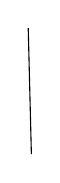
\begin{tikzpicture}[x=1cm,y=1cm]\draw (0,0)--(-0.04,1.6);\end{tikzpicture}}}
faut et il suffit qu'il existe un entier $n>0$, et un hom. de schémas en groupes $\varphi:\mathbb G_a\longrightarrow G$, tel qu'on ait
\[
(13)\qquad \varphi(1)=g^n.
\]

La suffisance étant triviale, il s'agit d'examiner la nécessité. Pour simplifier, on va encore supposer $S$ noethérien et intègre --- une fois $S$ supposé noethérien, je pense que la réduction au cas intègre doit se faire par des dévissages faciles, que je n'ai pas envie de faire, faute de besoin essentiel ! Je vais donc examiner le cas $S$ noeth. intègre, pt générique $\eta$

a) Car. \unsure{de} $\eta$ est $>0$. Alors \deleted{$\unsure{g_\eta}$} l'hypothèse sur $g_\eta$ est que $g_\eta$ est d'ordre fini --- donc $\exists n>0$ tel que $g_\eta^n=1$, donc $g^n=1$. On prendra dans (13) cet $n$, et $\varphi$ l'hom. trivial.

b) Cas où $\eta$ de car. nulle. Soit $\varphi$
\[
(14)\qquad \varphi_{1\eta}:\mathbb G_{a\eta}\longrightarrow G_\eta
\]
défini par la condition
\[
g_\eta=\varphi_{1\eta}(1)
\]
soit $U_1$ son ``ouvert de définition'' dans $S$.

Soit
\[
\varphi_{n\eta}(\lambda)=\lambda^n=\varphi_{1\eta}(n\lambda):\mathbb G_{a\eta}\longrightarrow G_\eta
\]
et soit $U_n$ son ouvert de définition. On a donc
\[
(15)\qquad\varphi_{n\eta}(1)=g^n\quad\text{sur }U_n
\]
\margin{10}

% Pied de page imprimé de l'archive.
\begin{center}
\small
10\\
\texttt{https://grothendieck.umontpellier.fr}\\
Université de Montpellier, UMR CNRS 5149, Case courrier 051, Place Eugène Bataillon\\
34095 Montpellier cedex 5 - France
\end{center}
\scanpage{12}
\deleted{\mspage{653}}
et
\[
(16)\qquad n\mid n'\quad\Longrightarrow\quad U_n\subset U_{n'}.
\]
Il faut prouver que la réunion des $U_n$ est $S$. On est ramené au cas $S$ local, et où $\varphi_1$ est déjà défini dans
\[
(17)\qquad U_1=S\setminus\{s\},\qquad s\text{ le pt fermé de }S
\]
et cela revient au

\margin{\unsure{à}}
\uline{Lemme} (!) \unsure{Soient} $S$ noeth. intègre, $G$ schéma en groupes \inserted{séparé} loc. de prés. finie sur $S$, $U$ ouvert non vide de $S$, $\varphi_U:\mathbb G_{aU}\longrightarrow G_U$ un hom. de groupes, on suppose que $\varphi_U(1)=g_U$ se prolonge en une section $g$ de $G$ sur $S$ tt entier (\unsure{néc\textsuperscript{t}.} unipotente, d'après des résultats connus généraux \unsure{de|du} SGA 3) Alors il existe un entier $>0$ tel que $\varphi_U^n:\lambda\longmapsto\varphi_U(\lambda^n)$ se prolonge \unsure{à|en} $S$ un hom.
\[
\varphi_n:\mathbb G_a\longrightarrow G.
\]

Je ne vais pas essayer de le démontrer dans ce contexte général des schémas en groupes généraux, et vais me limiter, à titre de test décisif (pour emporter conviction que \unsure{ça marche}) le cas où $G=\mathrm{Gl}(n)_S$, comme tantôt, et celui où $S$ de plus est régulier de dim 1.

Donc on est ramené à la situation d'une \unsure{jauge} $A$, et de $X\in M_n(K)$ ($K$ corps des fractions) satisfaisant
\margin{11}

% Pied de page imprimé de l'archive.
\begin{center}
\small
11\\
\texttt{https://grothendieck.umontpellier.fr}\\
Université de Montpellier, UMR CNRS 5149, Case courrier 051, Place Eugène Bataillon\\
34095 Montpellier cedex 5 - France
\end{center}
\scanpage{13}
\mspage{\textcircled{654}}
\[
(18)\qquad
\left\{\begin{array}{l}
X\in M_n(K)\\
X^n=0,\quad\displaystyle\sum\frac{X^i}{i!}\in M_n(A),\quad
\displaystyle\sum\frac{(-1)^iX^i}{i!}\in M_n(A)
\end{array}\right.
\]
et on veut montrer qu'il existe un entier $d>0$ tel qu'on ait
\[
(19)\qquad\frac{d^iX^i}{i!}\in M_n(A)\qquad(1\leq i\leq n-1)
\]
Si $A$ est de car 0 i.e. s'il est une $\mathbb Q$-algèbre, ceci \deleted{implique} \inserted{est équivalent} d'ailleurs :
\[
\frac{X^{\deleted{\unsure{i|0}}}}{\deleted{\unsure{i!}}}\in M_n(A)
\qquad\deleted{\text{\illegible{1}}\ X^i\in M_n(A))}
\]
\margin{\figure{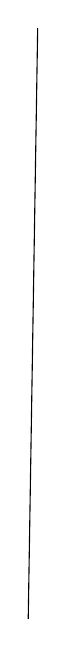
\begin{tikzpicture}[x=1cm,y=1cm]\draw (0,0)--(0.12,7.5);\end{tikzpicture}}}
\margin{le cas de car. nulle se résoud par l'affirmative à l'aide de la fonction logarithme --- posant
\[
X+\frac{X^2}{2!}+\cdots+\frac{X^{n-1}}{(n-1)!}=Y,
\]
on aura
\[
\exp X=1+Y,\quad\text{donc}
\]
\[
X=\log(1+Y)=Y-\frac{Y^2}{2}+\frac{Y^3}{3}\ldots
\]
Marche sur un anneau de base quelconque de car nulle\ldots}
\margin{$\unsure{b|0}$}
i.e. Il faudrait que dans le cas de car. 0, c'est $\varphi_U$ lui-$\overline{\mathrm m}$ qui puisse déjà se prolonger à $S$ tout entier. Le premier cas douteux à ce sujet me semble $\unsure{n|m}=5$
\[
(20)\qquad\left\{\begin{array}{l}
\deleted{\unsure{X^5=0}}\quad\inserted{X\in M_5(\unsure{A|K}),\ X^5=0}\\
\displaystyle\frac{X^2}{2}\pm\frac{X^3}{3!}+\frac{X^4}{\deleted{\unsure{2}}4!}\in M_5(A)\\[3pt]
\overset{?}{\Longrightarrow}\quad\deleted{\unsure{X^2,X^3,X^4}}\quad X\in M_5(A)
\end{array}\right.
\]

Par contre, dans le cas envisagé \unsure{un peu précédemment} ($n=4$, car. résiduelle 2 --- le seul qui fasse des difficultés) il est clair qu'il suffit de prendre pour $d$ une puissance de 2 assez grande.

Cette remarque s'applique aux cas d'inégales caractéristiques. On doit avoir en effet ceci

\uline{Corollaire au lemme} \unsure{dubitatif} : si $S$ est local, de car. résiduelle $p>0$, et si $\varphi$ est défini sur un ouvert qui contient $S-V(p)$, (i.e. si le complémentaire de $U$ est de car. $p\unsure{>|\geq}0$ --- en fait inutile bien sûr que $S$ soit local) alors $\exists q=p^{\unsure{r|n}}$ tel que $\varphi^q$ se prolonge.
\margin{12}

% Pied de page imprimé de l'archive.
\begin{center}
\small
12\\
\texttt{https://grothendieck.umontpellier.fr}\\
Université de Montpellier, UMR CNRS 5149, Case courrier 051, Place Eugène Bataillon\\
34095 Montpellier cedex 5 - France
\end{center}
\scanpage{14}
Quand $G$ est affine, ceci devrait être trivial. On va essayer la

\uline{Proposition} \unsure{Soient|Soit} $S$ un préschéma qu. cpt, $n$ un entier $\unsure{\geq1|\geq0}$, \deleted{\unsure{premier|prem.}} $S_0=V(n)\subset S$ le sous-schéma fermé défini par $n.1_S$ (donc si $x\in S$, on a $x\in S_0$ ssi \deleted{\unsure{car. $x$ est de}} \deleted{\unsure{car qui divise $n$}} \inserted{car $x\mid n$}), \inserted{$U=S\setminus S_0$,} $G$ un schéma en groupes affine \inserted{de \unsure{p.f.|t.f.}} sur $S$, et
\[
(21)\qquad\varphi_U:\mathbb G_a|U\longrightarrow G|U
\]
un hom. de groupes. \inserted{On suppose $U$ schématiquement dense dans $S$.} Alors il existe une \inserted{puiss.} entier \deleted{$d>0$} \inserted{$m=n^{\nu}$ de $n$,} \deleted{tel que} et un hom. de schémas en groupes
\[
\psi_m:\mathbb G_a\longrightarrow G\unsure{;|,}
\]
tel qu'on ait
\[
(22)\qquad\psi_m|U=\bigl(\varphi_U^m:\lambda\longmapsto\varphi_U(\unsure{m\lambda})=\varphi_U(\lambda)^m\bigr)
\]
Considérons en effet l'endom
\[
u_m:\mathbb G_a\longrightarrow\mathbb G_a\qquad\lambda\longmapsto m\lambda
\]
Alors la formule (22) signifie qu'on a commutativité
\diagram{\begin{tikzcd}
\mathbb G_{aU}\arrow[r,dash,"(u_m)_U"]\arrow[dr,"\psi_U"']&\mathbb G_{aU}\arrow[d,"\varphi_U"]\\
&G_U
\end{tikzcd}}
et l'existence des $\unsure{\psi_i|\psi_m}$ pour $m$ grand, signifie que pour $m$ grand l'hom. composé
\[
\deleted{\varphi_U\circ u_m}\qquad\varphi_U\circ u_m:\mathbb G_{aU}\unsure{\longrightarrow|\text{---}}G_U
\]
se prolonge en un hom. de groupes $\mathbb G_a\longrightarrow G$.
\margin{13}

% Pied de page imprimé de l'archive.
\begin{center}
\small
13\\
\texttt{https://grothendieck.umontpellier.fr}\\
Université de Montpellier, UMR CNRS 5149, Case courrier 051, Place Eugène Bataillon\\
34095 Montpellier cedex 5 - France
\end{center}
\scanpage{15}
\mspage{655}

Pour raisons de densité schématique et \unsure{unicité},
il suffit de prouver que $\varphi_U$ se prolonge en un
hom de schémas \deleted{en groupes} -- \inserted{ce} prolongement sera
automatiquement un hom de sch. en groupes.
\deleted{$A$ \unsure{celui de} \illegible{1} $B$}
\inserted{OPS $S$ \unsure{Affine}, \unsure{soit}}
$A$ \unsure{son} anneau, et soit $B$ celui de $G$.
Donc l'anneau de $U$ sera
\deleted{$A[1/n]\unsure{=}$}
$A_n\overset{\unsure{\mathrm{déf}}}{=}A[1/n]$, celui de $G$ sera
$B\otimes_A A_n=B_n$, par hyp on a un hom
(correspondant à $\unsure{\varphi_U^*|\varphi_U}$)
\[
(23)\qquad
\diagram{\begin{tikzcd}
B_n \arrow[r,"\varphi"] & A_n[T]
\end{tikzcd}}
\]
tandis que l'hom \deleted{\unsure{composé}}
\inserted{correspondant} à $\psi_{mU}$ sera le composé du précédent
avec
\[
(24)\qquad
\diagram{\begin{tikzcd}
A_n[T] \arrow[r,"\unsure{\psi_m^*|u_m^*}"] & A_n[T] \\
T \arrow[r,mapsto] & mT & \text{donc} & T^i \arrow[r,mapsto] & m^iT^i
\end{tikzcd}}
\]
Soit \deleted{$\unsure{x}$}
$\inserted{x=}\,a_0+a_1T+\cdots+a_NT^N\in A_n[T]$ \unsure{dont|donc} les
$a_i\in A_n$ on aura donc
\[
\psi_m^*(x)=\sum a_i m^iT^i=\sum(a_i n^{\unsure{i\nu}})T^i
\]
donc si $m=n^\nu$ est assez grand, on aura
\[
\deleted{\psi_m^*(x)\unsure{\sim}m^iT^i\in\unsure{A}}
\]
\[
m^i a_i\in A\quad\text{i.e}\quad m^i a_i\in\unsure{A|T^i}[T]
\qquad \forall i\,\uuline{\unsure{\ge|>}1}
\]
donc
\[
\psi_m^*(x)\equiv a_0\pmod{A[T]}
\]
ce qui montre
\[
(25)\qquad \psi_m(x)\in A[T]\ \text{pour }m=n^\nu\text{ grand}
\quad\Longleftrightarrow\quad a_0\in A
\]
\margin{14}

% Pied de page imprimé de l'archive.
\begin{center}
\small
14\\
\texttt{https://grothendieck.umontpellier.fr}\\
Université de Montpellier, UMR CNRS 5149, Case courrier 051, Place Eugène Bataillon\\
34095 Montpellier cedex 5 - France
\end{center}
\scanpage{16}

Appliquant ceci aux images d'éléments de $B$ qui engendrent $B$ comme
$A$-algèbre, on a donc

\uline{Corollaire}\quad $S$ \deleted{$\unsure{S_0}$} $n,S_0,U$ étant comme dans
la proposition, et $G$ étant un schéma affine de t.f. sur $S$
(il n'est plus question de structure de groupes), et
$\varphi_U:\mathbb E^1_U\longrightarrow G_U$ un hom de schémas,
\deleted{pour qu'il \unsure{existe}}
$g_U\,\deleted{\unsure{=}}\overset{\unsure{\mathrm{déf}}}{=}\varphi_U(0)$,
Pour qu'il existe une \deleted{\illegible{1}} puissance $m=n^\nu$
de $n$ telle que $\varphi_U\circ\unsure{\psi_m|u_m}$
\deleted{\unsure{(où}} (où $u_m$ donné par (24)) se prolonge
\inserted{à $S$}, il f et s. que $g_U$ se prolonge en une section $g$ de $G$
sur $S$.

\uline{Remarque}\quad les arguments précédents prouvent
en tous cas le "théorème" \unsure{dubitatif} p.\unsure{662|652}'
dans le cas où $S$ est noeth. de dim. 1
(le cas intéressant pour nous étant celui où le pt générique de $S$
est de car. 0).

\margin{\uline{Schémas en groupes} \uline{associés à des}
\unsure{ext. de} \uline{groupes discrets}}

3.\quad Soit maintenant $\unsure{M_0|M}$ un $\mathbb Z$-module
libre de type fini; on va construire un
pro-schéma en \uline{groupes} sur $S$, associé
au syst. projectif des sous-\deleted{groupes}\inserted{$\mathbb Z$}-modules
d'indice fini de $M$. Pour faire la
construction, je vais développer \deleted{\unsure{donc}} une
\margin{15}

% Pied de page imprimé de l'archive.
\begin{center}
\small
15\\
\texttt{https://grothendieck.umontpellier.fr}\\
Université de Montpellier, UMR CNRS 5149, Case courrier 051, Place Eugène Bataillon\\
34095 Montpellier cedex 5 - France
\end{center}
\scanpage{17}
\mspage{656}

\margin{Je me \unsure{complique} l'existence pour la construction de
$\underline{\mathfrak S}$, il suffit de poser
$\underline{\mathfrak S}=
\mathfrak S_{S_0}\times_{M_{S_0}}\underline M_{S_0}$.}

gamme préliminaire, relatif à une situation
\[
(26)\qquad
\diagram{\begin{tikzcd}
1 \arrow[r] & M \arrow[r] & \mathfrak S \arrow[r] & H \arrow[r] & 1
\end{tikzcd}}
\]
suite exacte de groupes discrets, avec $M$ commutatif --
le cas qui nous \unsure{intéressera} par la suite étant celui où $M$ est un
$\mathbb Z$-module libre de t.f. En tous cas $M$ est un
$\mathbb Z$-module, et à ce titre définit un Groupe sur
$\deleted{\unsure{\mathbb Z}}\inserted{\unsure{S_0}}=\operatorname{Spec}\mathbb Z$,
savoir
\[
\diagram{\begin{tikzcd}
A \arrow[r,mapsto] & M\otimes_{\mathbb Z}A
\end{tikzcd}}
\]
($A$, $\mathbb Z$-algèbre commutative) -- qu'on va désigner par $\underline M$.
En fait, $\underline M$ est représentable, i.e. est un \uline{schéma}
en groupes ssi $M$ est libre de type fini.
J'ai envie de définir aussi des \deleted{schémas en} Groupes sur $S_0$
(qui seront des schémas en groupes si $M$ l'est)
$\underline{\mathfrak S},\underline H$, et une suite exacte
\[
(27)\qquad
\diagram{\begin{tikzcd}
1 \arrow[r] & \underline M \arrow[r] &
\underline{\mathfrak S} \arrow[r] & \underline H \arrow[r] & 1
\end{tikzcd}}
\]
de Groupes sur $S_0$, et un isom des suites exactes
\[
(28)\qquad
\diagram{\begin{tikzcd}
1 \arrow[r] & M \arrow[r] \arrow[d,"\unsure{\wr}"] &
\mathfrak S \arrow[r] \arrow[d,"\unsure{\wr}"] &
H \arrow[r] \arrow[d,"\unsure{\wr}"] & 1 \\
1 \arrow[r] & \underline M(\mathbb Z) \arrow[r] &
\underline{\mathfrak S}(\mathbb Z) \arrow[r] &
\underline H(\mathbb Z) \arrow[r] & 1
\end{tikzcd}}
\]
on prendra
\[
(29)\qquad \underline H=H_{S_0}
\qquad\text{Groupe constant de val. }H
\]
et les flèches verticales extrêmes de (28)
\margin{16}

% Pied de page imprimé de l'archive.
\begin{center}
\small
16\\
\texttt{https://grothendieck.umontpellier.fr}\\
Université de Montpellier, UMR CNRS 5149, Case courrier 051, Place Eugène Bataillon\\
34095 Montpellier cedex 5 - France
\end{center}
\scanpage{18}

\unsure{seront|sont} les isom. canoniques.

On peut songer à définir $\underline{\mathfrak S}$ comme
foncteur \inserted{(cov.)} en $A/\mathbb Z$ ou (\unsure{contravariant})
en $S/S_0$, par
\[
(30)\qquad
\underline{\mathfrak S}(A)=
\mathfrak S\wedge_M
\underbrace{M(A)}_{\deleted{\unsure{A\otimes_{\mathbb Z}}}\inserted{M\otimes_{\mathbb Z}A}}
\]
\deleted{\unsure{Comme on a}}.
$\underline{\mathfrak S}(A)$ étant donc défini comme l'ext. de
$H$ par $M(A)$ \unsure{déduite} de l'ext. $\mathfrak S$
de $H$ par $M$ par l'hom
\[
(31)\qquad
\diagram{\begin{tikzcd}
M \arrow[r] & M\otimes_{\mathbb Z}A
\end{tikzcd}},
\]
qu'on considère comme un hom de $H$-$\mathbb Z$-modules,
en faisant opérer $H$ sur $M\otimes_{\mathbb Z}A$ via son opération sur $M$.

La petite difficulté est que le foncteur-\unsure{groupe|groupes}
ainsi défini par (30) n'est pas lui-$\overline{\mathrm m}$ représentable --
il ne donne l'expression correcte de $\underline{\mathfrak S}(A)$ que si
$\operatorname{Spec}A$ est connexe -- il correspond au sous-foncteur de
\[
\begin{array}{c}
\inserted{\unsure{\sim}}\\[2pt]
\diagram{\begin{tikzcd}
S \arrow[r,mapsto] &
\unsure{:}\underline{\mathfrak S}(A)=
\deleted{\unsure{\operatorname{Spec}|\underline{\mathfrak S}}}
\underline{\mathfrak S}(S)
\end{tikzcd}}
\qquad (S=\operatorname{Spec}A)
\end{array}
\]
formé des \deleted{pts tels que le}
\inserted{$S\longrightarrow\underline{\mathfrak S}$}
tels que le composé
\[
(32)\qquad
\diagram{\begin{tikzcd}
S \arrow[r] & \underline H_S
\end{tikzcd}}
\]
(qui correspond à une fonction \uuline{loc.} \uline{\unsure{constante|const.}}
sur $S$ à valeurs dans $H$) soit
\inserted{(\unsure{entièrement})} constante.
\margin{17}

% Pied de page imprimé de l'archive.
\begin{center}
\small
17\\
\texttt{https://grothendieck.umontpellier.fr}\\
Université de Montpellier, UMR CNRS 5149, Case courrier 051, Place Eugène Bataillon\\
34095 Montpellier cedex 5 - France
\end{center}
\scanpage{19}
\mspage{657}

L'expression correcte s'obtiendra en partant du \inserted{\illegible{1}} foncteur ``incorrect''
\[
\diagram{\begin{tikzcd}
{[\underline{\mathfrak S}]: A} \arrow[r,mapsto] &
\mathfrak S\wedge_M(M\otimes_{\mathbb Z}A)
\end{tikzcd}}
\]
\unsure{ou} mieux, du \unsure{contr. foncteur|contre-foncteur}
\[
\diagram{\begin{tikzcd}
S \arrow[r,mapsto] &
\mathfrak S\wedge_M
\Gamma(S,M\otimes_{\mathbb Z}\underline{\unsure{\mathcal O|O}}_S)
\end{tikzcd}},
\]
et en prenant le faisceau Zariski associé -- en fait on aura. $=$
\[
(33)\qquad
\underline{\mathfrak S}(S)=
\underset{\mathcal U=(U_i)_{i\in\unsure{S|I}}}{\varinjlim}
\prod_{i\in I}[\mathfrak S](U_i)
\]
\[
\begin{array}{l}
(U_i)_{i\in I}\ \text{une partition}\\
\text{de }S\text{ en }\unsure{\text{schém.}}\\
\unsure{\text{ouverts}}\qquad S\simeq\coprod U_i
\end{array}
\]

Voici une autre façon de présenter la construction de
$\underline{\mathfrak S}$, en utilisant la construction générale
du §49 -- dans le contexte faisceautique. On a un système
\[
(34)\qquad
\underbrace{\underline M}_{\text{Groupe sur }S_0},
\quad
\underbrace{\mathfrak S_{S_0}
\overset{\cdot}{\supset}\unsure{M}_{S_0}}_{
\substack{\text{Groupes (constants)}\\
\text{sur }S_0,\ M_{S_0}\\
\text{distingué}}},
\quad
\mathrm{Op.}^{\unsure{\Theta|\theta}}\text{ de }
\mathfrak S_{S_0}\text{ sur }\underline M,
\]
\[
\diagram{\begin{tikzcd}
\text{hom }\varphi:
\deleted{\unsure{\mathfrak S}}\inserted{M}_{S_0}
\arrow[r] & \underline M
\end{tikzcd}}
\]
(où l'op. de $\mathfrak S_{S_0}$ sur $\underline M$,
qui \unsure{revient} à une op. de $\mathfrak S$ sur $\underline M$,
est celle déduite de l'op. de $\mathfrak S$ sur $M$,
par \unsure{fonctorialité})
ces données \unsure{satisfaisant} aux conditions de compatibilité a) b)
de loc. cit. Par la construction \unsure{du|de} loc. cit., on construit
\margin{18}

% Pied de page imprimé de l'archive.
\begin{center}
\small
18\\
\texttt{https://grothendieck.umontpellier.fr}\\
Université de Montpellier, UMR CNRS 5149, Case courrier 051, Place Eugène Bataillon\\
34095 Montpellier cedex 5 - France
\end{center}
% ===== LM_C4-020-038: second pass, checked against the scans =====
\scanpage{20}

à l'aide \unsure{en se donnant} un système

\diagram{\begin{tikzcd}[column sep=large]
\text{(35)} &
\begin{gathered}
\underline{\mathcal G}\supset\underline M\\[-2pt]
\text{Groupe sur }S_0,\\[-2pt]
\text{avec }\underline M\text{ comme}\\[-2pt]
\text{sous-groupe distingué}
\end{gathered}
& \text{, et }\Phi\colon\mathcal G_{S_0}\arrow[r]
& \underline{\mathcal G}
\end{tikzcd}}

tel que (34) se \unsure{reconstitue} à partir de (35) en prenant
$\underline M$, $\mathcal G_{S_0}$ dans (35),
$M_{S_0}$ \deleted{\illegible{1}}$=$ l'image inverse de
$\underline M\subset\underline{\mathcal G}$ par $\Phi$,
$\varphi$ induit par $\Phi$, et $\Theta$ l'opération déduite de
$\Phi$. De plus, $\Phi$ induit un \uline{iso}.

\diagram{\begin{tikzcd}
\underbrace{\mathcal G_{S_0}/M_{S_0}}_{H_{S_0}}
\arrow[r,"\sim"] & \underline{\mathcal G}/\underline M
\end{tikzcd}}

-- et on a là une description ``axiomatique'' du système (35)
en termes de (34).
La suite exacte de \deleted{\unsure{schémas}}\inserted{Groupes sur $\unsure{S|S_0}$}

\diagram{\begin{tikzcd}[column sep=large,row sep=small]
\text{(36)} & 1\arrow[r,dash] & \underline M\arrow[r]
& \underline{\mathcal G}\arrow[r]
& \underline{\mathcal G}/\underline M\arrow[r,dash]
\arrow[d,phantom,"\simeq"{description,rotate=90}] & 1\\
&&&& H_{S_0}.
\end{tikzcd}}

de fait, sur $\forall$ schém. de base affine $S$
(plus généralement, $S$ tel que $H^1(S,M\otimes_{\mathbb Z}\underline{\mathcal O}_S)=0$)
\unsure{des} suites exactes

\margin{L'hyp. \unsure{faite} sur des $H^1$ \unsure{nul|nuls}
est entièrement inutile, car les $\underline M$-torseurs
\uline{sur} $S_0$ définis par les \unsure{images} \unsure{inverses}
des $h(\in H)$ sont évidemment triviaux}

\diagram{\begin{tikzcd}[column sep=large,row sep=small]
\text{(37)} & 1\arrow[r] & \underline M(S)\arrow[r]
\arrow[d,phantom,"\simeq"{description,rotate=90}]
& \underline{\mathcal G}\unsure{(A)|(/A)}\arrow[r]
& H_{S_0}(S)\arrow[r,dash]
\arrow[d,phantom,"\simeq"{description,rotate=90}] & 1\\
&& M\otimes_{\mathbb Z}A && H\text{ si }S\text{ conn.}\\[-3pt]
&&\text{si }S\text{ affine d'anneau }A
\end{tikzcd}}

\margin{19}
\scanpage{21}
\mspage{658}

En fait, on a par construction un \unsure{diagramme}
comm. de suites exactes

\diagram{\begin{tikzcd}[column sep=large,row sep=large]
\text{(38)} & 1\arrow[r] & M_{S_0}\arrow[r]\arrow[d]
&\mathcal G_{S_0}\arrow[r]\arrow[d]
&H_{S_0}\arrow[r,dash]
\arrow[d,phantom,"\unsure{\Downarrow}"{description}] &1\\
&1\arrow[r]&\underline M\arrow[r]
&\underline{\mathcal G}\arrow[r]&H_{S_0}\arrow[r]&1
\end{tikzcd}}

qui par passage aux sections donne \deleted{pour} $S$
\deleted{quelconque} affine (disons) connexe un diag. comm.

\diagram{\begin{tikzcd}[column sep=large,row sep=large]
\text{(39)} &1\arrow[r]&M\arrow[r]\arrow[d]
&\mathcal G\arrow[r]\arrow[d]
&H\arrow[r]\arrow[d,phantom,"\unsure{\Downarrow}"{description}]&1\\
&1\arrow[r]&M\otimes_{\mathbb Z}A\arrow[r]
&\underline{\mathcal G}(A)\arrow[r,dash]&H\arrow[r,dash]&1.
\end{tikzcd}}

Pour $S=S_0$ on retrouve l'iso (28) annoncé.

\margin{\uline{NB} En tant que faisceau (\unsure{sans} structure de
$S$-groupes) $\underline{\mathcal G}$ est isomorphe au
\deleted{\unsure{schéma}}\inserted{faisceau} somme des $H$ copies de
$\underline M$ -- il est donc représentable si $\underline M$ l'est.}

Cette construction du $\unsure{S_0}$-schéma en groupes
$\underline{\mathcal G}$, à partir d'une suite exacte (27), est
\unsure{manifestement} fonctorielle \unsure{p.r.|par.} à cette dernière :
un \unsure{hom.} de suites exactes

\diagram{\begin{tikzcd}[column sep=large,row sep=large]
\text{(40)}&1\arrow[r]&M\arrow[r]\arrow[d]
&\mathcal G\arrow[r]\arrow[d]&H\arrow[r]\arrow[d]&1\\
&1\arrow[r]&M'\arrow[r]&\mathcal G'\arrow[r]&H'\arrow[r,dash]&1
\end{tikzcd}}

donne naissance à un diag. comm. de suites exactes

\margin{20}
\scanpage{22}

\diagram{\begin{tikzcd}[column sep=small,row sep=large]
&1\arrow[rr,dash]&&M_{S_0}\arrow[rr]\arrow[dr]\arrow[dd]
&&\mathcal G_{S_0}\arrow[rr]\arrow[dr]\arrow[dd]
&&H_{S_0}\arrow[rr,dash]\arrow[dr]
\arrow[dd,dash,"\unsure{\Vert}"{description,pos=.25}]
&&1&\\
&&1\arrow[rr,crossing over]
&&M'_{S_0}\arrow[rr]\arrow[dd]
&&\mathcal G'_{S_0}\arrow[rr]\arrow[dd]
&&H'_{S_0}\arrow[rr]\arrow[dd]&&1\\
\text{(41)}&1\arrow[rr]&&\underline M^{\unsure{\cdot}}\arrow[rr]\arrow[dr]
&&\underline{\mathcal G}\arrow[rr]\arrow[dr]
&&H_{S_0}\arrow[rr]\arrow[dr]&&1&\deleted{\unsure{1}}\\
&&1\arrow[rr]&&\underline M'\arrow[rr]
&&\underline{\mathcal G}'\arrow[rr]
&&\underline H'\arrow[rr]&&1
\end{tikzcd}}

\margin{\uline{Enveloppe schématique} \uline{discrète}
\uline{des groupes} \uline{métabéliens}}

4. Reprenons donc un $\mathbb Z$-module libre de type fini $M$, et pour
$\forall$ sous-\deleted{\unsure{g}}\inserted{$\mathbb Z$}-module
d'indice fini, considérons la suite exacte

\diagram{\begin{tikzcd}[column sep=large]
\text{(41)}&1\arrow[r,dash]&M_i\arrow[r,dash]&M\arrow[r,dash]
&M/M_i\arrow[r,dash]&1.
\end{tikzcd}}

Plus \unsure{gén.}, si on part d'une suite exacte (27), pour
$\forall$ sous-groupe $M_i$ d'indice fini dans $M$,
\unsure{distingué} dans $\mathcal G$ i.e. stable par $H$,
on a une suite exacte

\diagram{\begin{tikzcd}[column sep=large]
\text{(43)}&1\arrow[r]&M_i\arrow[r]&\mathcal G\arrow[r]
&\underbrace{\mathcal G/M_i}_{H_i}\arrow[r,dash]&1
\end{tikzcd}}

où maintenant $H_i=\mathcal G/M_i$ \unsure{est} \unsure{l'|une}
extension de

\diagram{\begin{tikzcd}[column sep=large]
\text{(44)}&1\arrow[r]&M/M_i\arrow[r]&H_i\arrow[r]&H\arrow[r]&1
\end{tikzcd}}

déduite de (27) par

\diagram{\begin{tikzcd}
M\arrow[r]&M/M_i.
\end{tikzcd}}

\margin{21}
\scanpage{23}
\mspage{659}

On note que \deleted{si $H$ est un groupe \unsure{ayant} un
\unsure{nb} fini de \unsure{gén.}, pour $H$ fini},
\deleted{alors} les $M_i\subset M$ d'indice fini et stables sous $H$
sont cofinaux dans l'\unsure{ens} de tous les $M_i$ d'indice fini dans
$M$. Considérons donc la suite exacte de sch. en groupes associée

\margin{prendre les $nM$ !}

\diagram{\begin{tikzcd}[column sep=large]
\text{(45)}&1\arrow[r]&\underline{M_i}\arrow[r]
&\underline{\mathcal G}_i\arrow[r]&H_{i\,S_0}\arrow[r]&1
\end{tikzcd}}

Pour $i$ variable, elles forment un syst. projectif d'extensions,
donc une extension de \unsure{progroupes} sur $S_0=\operatorname{Spec}\mathbb Z$.

\deleted{En particulier}

\deleted{\uline{\unsure{Remarque|Le pro-groupe}} $\unsure{\underline{\mathcal G}}$}

On considère le pro-objet $(\underline{\mathcal G}_i)$ comme pro-objet
de $C$ catégorie des schémas en groupes (lisses etc ...) sur $S_0$.
On note que les morphismes de transition

\diagram{\begin{tikzcd}
\underline{\mathcal G}_j\arrow[r]&\underline{\mathcal G}_i
\end{tikzcd}}

sont \uline{affines} -- la question étant locale
\inserted{sur $\underline{\mathcal G}_i$}, on est ramené à la voir pour
l'hom

\deleted{\unsure{image}}

\diagram{\begin{tikzcd}[column sep=large,row sep=small]
\unsure{E}(M_i,M_j)\arrow[r]
&E(M_i,M_i)\arrow[d,phantom,"\unsure{\Vert}"{description}]\\
M_i\supset M_j&\underline{M_i}\\[-3pt]
\text{ext. de }(M_i/M_j)_{S_0}\text{ par }\underline{M_j}
\end{tikzcd}}

\margin{22}
\scanpage{24}

Or le premier est affine, comme somme finie de schémas affines, le deuxième est affine --- donc le morphisme est affine.

Ceci étant, la limite projective des $\underline{\mathcal{G}}_i$ dans la catégorie des schémas existe (plus précisément, le foncteur limite projective des $\underline{\mathcal{G}}_i$ est représentable) --- il n'est peut être pas absurde de passer à la limite \unsure{carrément}, et de travailler avec ce schéma en groupes --- pas de t.f.

\uline{Remarque} Le pro-groupe $(\underline{\mathcal{G}}_i)$ sur $S_0=\operatorname{Spec}\unsure{\mathcal{G}|\mathbb{Z}}$ ne dépend que du \deleted{$\mathcal{G}$}, groupe discret $\mathcal{G}$, muni d'une classe de sous-groupes \inserted{\deleted{\unsure{invariants} abéliens}} modulo commensurabilité --- l'hypothèse à faire étant que parmi ces sous-groupes, il y en a qui sont des $\mathbb{Z}$-modules \deleted{libres} de type fini (car les prenant assez petits, ils sont \uline{libres} de t.f.). Si $M_0$ est lui-$\overline{\mathrm m}$ d'indice fini dans $\mathcal{G}$ i.e. si \deleted{les}\inserted{\unsure{un des|$\forall$ des}} $H_i$ sont finis,

\margin{23}
\scanpage{25}
\mspage{660}

alors ce proobjet ne dépend que de $\mathcal{G}$ lui
$\overline{\mathrm m}$ --- \unsure{soumis} à la condition qu'il existe
un sous-groupe d'indice fini dans $\mathcal{G}$ qui
soit un groupe commutatif, de t.f. en
tant que $\mathbb{Z}$-module. (On dit alors
que $\mathcal{G}$ est "\uline{métabélien}".)

\margin{\unsure{3}}
\deleted{Regardons le cas typique}

Ainsi, pour $\forall$ groupe discret
\inserted{$\mathcal{G}$} métabélien, on a construit un proschéma
en groupes, \inserted{syst. proj. de schémas en groupes \uline{affines},}
que je vais noter
\[
(46)\qquad
\operatorname{Env}(\mathcal{G})=(\underline{\mathcal{G}}_i)
\]
(l'ens d'indices étant formé des sous-groupes
distingués de $\mathcal{G}$ qui sont comm. et sans
torsion). Ce pro-groupe dépend \unsure{fonctoriellement}
de $\mathcal{G}$. Il a des propriétés \unsure{d'exactitudes|d'exactitude}
\unsure{intéressantes} et $\pm$ évidentes, p. ex.
il est multiplicatif
\[
(47)\qquad
\operatorname{Env}(\mathcal{G}\times\mathcal{G}')
\unsure{\xrightarrow{\sim}}
\operatorname{Env}(\mathcal{G})\mathbin{\times_{S_0}}
\operatorname{Env}(\mathcal{G}').
\]
Si on a une suite exacte
\[
(48)\qquad
\diagram{\begin{tikzcd}[column sep=large]
1 \arrow[r] & \mathcal{G}'' \arrow[r,no head] &
\mathcal{G} \arrow[r,no head] & \mathcal{G}' \arrow[r,no head] & 1
\end{tikzcd}}
\]
de groupes métabéliens, on a une suite
exacte pour les enveloppes
\[
(49)\qquad
\diagram{\begin{tikzcd}[column sep=large]
1 \arrow[r] & \unsure{\operatorname{Env}}(\mathcal{G}'') \arrow[r] &
\operatorname{Env}(\mathcal{G}) \arrow[r,no head] &
\operatorname{Env}(\mathcal{G}') \arrow[r] & \unsure{1}
\end{tikzcd}}
\]

\margin{24}
\scanpage{26}

en un sens qu'il convient de préciser \unsure{à}
l'occasion --- pour les schémas en groupes
associés (obtenus en passant à la limite) ---
\unsure{on a bel et bien} un hom fid plat dont
le noyau est le bon \ldots

Le cas typique, auquel le cas général
se ramène de façon \unsure{assez} immédiate, est
celui où $\mathcal{G}=M=\mathbb{Z}$. On a pour
$\forall$ entier $n\geq 1$ la suite exacte
\[
(50)\qquad
\diagram{\begin{tikzcd}[column sep=large]
1 \arrow[r,no head] &
\mathbb{Z} \arrow[r,no head,"n"] &
\mathbb{Z} \arrow[r,no head] &
\mathbb{Z}/n\mathbb{Z} \arrow[r,no head] & 1
\end{tikzcd}}
\]
je vais \deleted{\unsure{construire}} expliciter la construction
de l'extension correspondante de
$\mathbb{Z}/n\mathbb{Z}$ par $\underline{\mathbb{Z}}=\mathbb{G}_a$,
soit $\underline{\mathcal{G}}_n$.

C'est un schéma affine, dont l'anneau
de coordonnées est isomorphe --- de façon pas
bien canonique --- au produit des
$n$ copies de celui de $\underline{\mathbb{Z}}=\mathbb{G}_a$,
savoir $\mathbb{Z}[T]$ --- on trouve un tel \unsure{isomorphisme}
en \unsure{choisissant} une section ensembliste de
$\mathbb{Z}$ sur $\mathbb{Z}/n\mathbb{Z}$, par exemple par \unsure{l'ens}
des entiers $\mathbb{Z}\cap[0,n-1]$. Les hom de

\margin{25}
\scanpage{27}
\mspage{661}

transition entre les $\underline{\mathcal{G}}_n$ n'ont rien de
plat bien sûr. Passant à la limite projective,
on trouve une extension de
\[
(\widehat{\mathbb{Z}})_{S_0}
\overset{\mathrm{dfn}}{=}
\varprojlim_n(\mathbb{Z}/n\mathbb{Z})_{S_0}
\]
--- schéma en groupes profini constant sur $S_0$ ---
par la limite projective des schémas
$\mathbb{G}_a$, s'envoyant dans lui $\overline{\mathrm m}$
par les hom
\unsure{vus} \deleted{\unsure{des} \unsure{\S b}} de $2^\circ$)
--- c'est le spectre
de l'anneau limite inductive des
\[
\begin{gathered}
\mathbb{Z}[T_n]\subset\mathbb{Q}[T]\\
T_n=\frac{1}{n}T
\end{gathered}
\]
qui est ainsi, chose étrange, \unsure{la} \deleted{\illegible{1}}
\inserted{\unsure{sous-}}$\mathbb{Z}$-algèbre
de $\mathbb{Q}[T]$ \unsure{formé|formée} des polynômes
dont \uline{le terme constant} est un entier.

On a une \unsure{description} analogue de
la limite projective de l'enveloppe
schématique de $\mathbb{Z}^n$ --- c'est une
extension de $(\widehat{\mathbb{Z}}^{\,n})_{S_0}$
(attention à l'abus
de notation) par une composante neutre,
qui est le spectre du sous-anneau
de $\mathbb{Q}[T_1,\ldots,T_n]$ formé des polynômes dont
le terme constant est entier \ldots

\margin{26}
\scanpage{28}

C'est donc un schéma en groupes sur $S_0=\operatorname{Spec}\mathbb{Z}$
dont toutes les fibres sont réduites au groupe
unité, sauf la fibre \unsure{générique}, qui est
$ {\mathbb{G}_a^{\,n}}_{\mathbb{Q}}$.

\deleted{\unsure{Et}}
Dans le cas d'un groupe métabélien
quelconque $\mathcal{G}$, \unsure{désignant|désignons} par
$\widehat{\mathcal{G}}$ son
\unsure{complétifié} profini, par $\widehat{\mathcal{G}}_{S_0}$ le schéma
en groupes profini sur $\unsure{S_0}$.
\[
(50)\qquad
\widehat{\mathcal{G}}_{S_0}
\overset{\mathrm{dfn}}{=}\varprojlim_i(H_i)_{S_0}
\]
on \unsure{en} aura une suite exacte canonique
\[
(51)\qquad
\diagram{\begin{tikzcd}[column sep=large]
1 \arrow[r] &
\operatorname{Env}^{0}(\mathcal{G})
\arrow[r,very thick,"\deleted{\unsure{\mathrm{dfn}}}"] &
\varprojlim\operatorname{Env}(\mathcal{G}) \arrow[r] &
(\widehat{\mathcal{G}})_{S_0} \arrow[r] & 1
\end{tikzcd}}
\]
où $\operatorname{Env}^{0}(\mathcal{G})$ désigne la comp. neutre
de $\unsure{\varprojlim}\operatorname{Env}(\mathcal{G})$, i.e.
\[
\begin{aligned}
(52)\qquad
\operatorname{Env}^{0}(\mathcal{G})
&\overset{\mathrm{dfn}}{=}\varprojlim_i\underline{M}_i\\
&\simeq\varprojlim_n n.\,\underline{M}_0
\end{aligned}
\]
où les $M_i$ sont les sous-groupes d'indice
fini de $\mathcal{G}$ \deleted{\unsure{tels q|tel q}}
qui sont des $\mathbb{Z}$-modules libres de t.f., où
(comme plus haut) pour un tel $\mathbb{Z}$-module $M$,

\figure{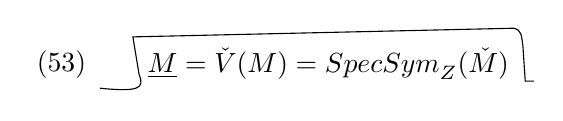
\begin{tikzpicture}[baseline=(eq.base)]
\node[anchor=base west,inner sep=0pt] (eq) at (0,0)
{$\underline{M}=\check{V}(M)=\operatorname{Spec}\operatorname{Sym}_{\mathbb{Z}}(\check{M})$};
\node[anchor=east] at ([xshift=-0.65cm]eq.west) {$(53)$};
\draw
([xshift=-0.60cm,yshift=-0.10cm]eq.south west)
.. controls ([xshift=-0.10cm,yshift=-0.15cm]eq.south west)
and ([xshift=-0.03cm,yshift=-0.10cm]eq.south west)
.. ([xshift=-0.10cm,yshift=0.07cm]eq.south west)
-- ([xshift=-0.18cm,yshift=0.14cm]eq.north west)
-- ([xshift=0.05cm,yshift=0.25cm]eq.north east)
.. controls ([xshift=0.16cm,yshift=0.23cm]eq.north east)
and ([xshift=0.15cm,yshift=0.15cm]eq.north east)
.. ([xshift=0.17cm,yshift=0.03cm]eq.north east)
-- ([xshift=0.20cm,yshift=-0.01cm]eq.south east)
-- ([xshift=0.31cm,yshift=-0.01cm]eq.south east);
\end{tikzpicture}}
désigne le fibré-vectoriel \unsure{cov.|can.} en $M$ qu'il définit, et

\margin{27}
\scanpage{29}
\mspage{662}

où $M_0$ est un des $M_i$, donnant lieu
au syst. (cofinal dans celui de tous les
$M_i$) des $nM_0$. Le choix d'une
base de $M_0$ sur $\mathbb{Z}$ donne un
iso
\[
(54)\qquad
\begin{aligned}
\operatorname{Env}^{0}(\mathcal{G})
&\simeq \operatorname{Env}^{0}(M_0)
\simeq \bigl(\operatorname{Env}^{0}(\mathbb{Z})^{\unsure{0}}\bigr)^n\\
&\simeq(\mathcal{E}^{1})^n
\end{aligned}
\]

\margin{$\unsure{\dagger}$ où
\diagram{\begin{tikzcd}[column sep=large]
(\mathbb{E}^{1},\unsure{mn|nm}) \arrow[r] &
(\mathbb{E}^{1},\uuline{n})
\end{tikzcd}}
est la multiplication par $m$}

\[
(55)\qquad
\begin{aligned}
\mathcal{E}^{1}
&\simeq \operatorname{Env}^{0}(\mathbb{Z})
\simeq\operatorname{Spec}\bigl(\mathbb{Z}+T\mathbb{Q}[T]\bigr)\\
&\inserted{\simeq\varprojlim_n(\mathbb{E}^{1},n)\,\unsure{\dagger}}
\end{aligned}
\]
est le schéma en groupes envisagé plus
haut, qui représente le foncteur en groupes
\[
(56)\qquad
A\longmapsto\mathcal{E}^{1}(A)
=\deleted{\unsure{\varprojlim}}
\left\{(x_n)\in A^{\mathbb{N}^{*}}\ \middle|\
\begin{gathered}
x_n=mx_{mn}\\[-2pt]
\forall m,n\in\unsure{\mathbb{N}^{*}}
\end{gathered}
\right\}.
\]

[Si $A$ est tel qu'il existe $n\in\mathbb{N}^{*}$ avec
$nA\,\unsure{=|\simeq}\,0$ ---
\deleted{\unsure{précis.}}
ce qui signifie
que les car. résiduelles de $A$ divisent $n$,
et \deleted{\unsure{c'est}} il existe sans doute un tel $n$
dès que les car. résiduelles de $A$ sont
toutes $>0$ --- alors $\mathcal{E}^{1}(A)=\{1\}$ ---
si par contre $A$ de car $0$, on a $\mathcal{E}^{1}(A)\simeq A$]

\margin{28}
\scanpage{30}

5. \uline{Caractérisation universelle} de l'enveloppe schématique d'un groupe métabélien.

Soit $G$ un schéma en groupes \unsure{loc.} de prés. finie sur une base $S$.
On dit qu'un \unsure{hom.} de schémas en groupes
\diagram{\begin{tikzcd}
H \arrow[r] & G
\end{tikzcd}}
est \deleted{\unsure{quasi-}} \uline{unipotent} (resp. quasi-unipotent) si l'image de $\forall$ \unsure{élt} de $H$ est un élément unipotent (resp. quasi unipotent) de $G$ --- ce qui se vérifie fibre par fibre. Un \unsure{hom.} d'un groupe discret
\diagram{\begin{tikzcd}
\mathcal{G} \arrow[r] & \Gamma(G/S)
\end{tikzcd}}
est dit unipotent (resp. quasi-unipotent) si l'\unsure{hom.} des schémas en groupes \deleted{\unsure{associé}} \inserted{qui} lui correspond
\diagram{\begin{tikzcd}
\mathcal{G}_S \arrow[r] & G
\end{tikzcd}}
est unipotent (resp. quasi-unipotent).

\margin{29}
\scanpage{31}
\mspage{663}

Notons que d'après les propriétés des $\varprojlim$ de syst. projectifs filtrants (à morphismes de transition affines) \deleted{entre} de schémas, si $\mathcal{G}$ est métabélien, d'où un système projectif de schémas en groupes affines sur $S_0$, donc sur $S$, noté $\operatorname{Env}_{\unsure{\underline{S}|S}}(\mathcal{G})$, et une limite projective
\[
\begin{aligned}
(57)\qquad L\operatorname{Env}_S(\mathcal{G})
 &=L\operatorname{Env}(\mathcal{G})\times_{S_0}S\\
 &\simeq\varprojlim\operatorname{Env}_S(\mathcal{G}),
\end{aligned}
\]
on a, dès que $G$ est \unsure{loc.} de prés. finie

(58)\quad
\diagram{\begin{tikzcd}[column sep=large,row sep=large]
\operatorname{Hom}_{\mathrm{progr}/S}(\operatorname{Env}_S(\mathcal{G}),G)
 \arrow[r,"\sim"] \arrow[d,equal,"\mathrm{def}"']
 & \operatorname{Hom}(\operatorname{Env}_S(\mathcal{G}),G)\\
\varprojlim_i\unsure{\operatorname{Hom}}(\underline{\mathcal{G}}_{i\,S},G) &
\end{tikzcd}}

Notons d'autre part qu'on a un \deleted{\unsure{un}} \unsure{hom.} canonique

(59)\quad
\diagram{\begin{tikzcd}
\mathcal{G}_S \arrow[r] & \deleted{\unsure{\varprojlim}}L\operatorname{Env}_S(\mathcal{G})
\end{tikzcd}}
déduit par \unsure{changement} de base de l'\unsure{hom.} sur la base universelle $S_0$

(59 bis)\quad
\diagram{\begin{tikzcd}
\mathcal{G}_{S_0} \arrow[r] & L\operatorname{Env}(\mathcal{G})
\end{tikzcd}}
provenant du système d'\unsure{hom.} can.

\margin{30}
\scanpage{32}

\diagram{\begin{tikzcd}
\underline{\mathcal{G}}_{S_0}\arrow[r]&\underline{\mathcal{G}}_i
\end{tikzcd}}.

Donc, via (59) on trouve

(60)\quad
\diagram{\begin{tikzcd}[column sep=large,row sep=large]
\operatorname{Hom}_{S\text{-}\mathrm{gr}}(L\operatorname{Env}_S(\mathcal{G}),G)
 \arrow[r] & \operatorname{Hom}_{S\text{-}\mathrm{gr}}(\mathcal{G}_S,G)
 \arrow[d,phantom,"\simeq"{rotate=90}]\\
 & \operatorname{Hom}_{\mathrm{gr}}(\mathcal{G},\Gamma(G/S))
\end{tikzcd}}

\unsure{1}

\unsure{Composant} (58) et (60), on trouve
\[
(61)\quad\left\{
\begin{aligned}
&\operatorname{Hom}_{\mathrm{pro}\text{-}S\text{-}\mathrm{gr}}\unsure{\ell}
 (\operatorname{Env}_S(\mathcal{G}),G)
 \simeq\operatorname{Hom}_{S\text{-}\mathrm{gr}}(L\operatorname{Env}_S(\mathcal{G}),G)\\[1.2em]
&\hspace{5em}\longrightarrow\operatorname{Hom}_{S\text{-}\mathrm{gr}}(\mathcal{G}_S,G)
 \simeq\operatorname{Hom}_{\mathrm{gr}}(\mathcal{G},G(S))
\end{aligned}\right.
\]
Ceci posé, on a le résultat suivant

\uline{Théorème} \deleted{\unsure{Si}} Sous les conditions précédentes

\margin{\figure{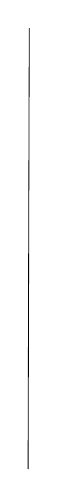
\begin{tikzpicture}
\draw[line width=.3pt] (0,0) -- (-.015,-5.6);
\end{tikzpicture}}}
($\mathcal{G}$ groupe discret métabélien, $G$ schéma en groupes loc. de prés. finie sur \unsure{schéma} de base $S$), l'application canonique (61) est \deleted{\uline{bijective} si on suppose de plus, pour ne pas \unsure{me|se} fatiguer, que} \inserted{injective, et a comme image} \unsure{l'ens.} des \unsure{hom.} \uline{quasi-unipotents} de $\mathcal{G}$ dans $G(S)$ --- du moins si on suppose, pour nous simplifier l'existence, que $S$ est \unsure{noeth.} et $G$ affine sur $\unsure{S|S_0}$.

\margin{31}
\scanpage{33}
\mspage{664}

\uline{5\unsure{1|0}} \uline{Exemple} : La ``tour'' de Fermat.

1. Les groupes $\mathcal{G},\underline{\mathcal{G}}$.

Je m'intéresse au quotient de $\mathcal{G}_0^{\deleted{\unsure{\wedge}}}=\operatorname{GL}(2,\mathbb{Z})$ obtenu en prenant le quotient par $[\Pi_0,\Pi_0]$ --- on trouve une extension $\mathcal{G}$ de $\mathcal{G}_0/\Pi_0$ par le groupe

\margin{$\Pi_0$ engendré par les $\lambda_i=-\ell_i$,\quad
$\displaystyle \ell_0=\begin{pmatrix}1&-2\\0&1\end{pmatrix}$\quad
$\displaystyle \ell_1=\begin{pmatrix}1&0\\2&1\end{pmatrix}$.}

\[
\begin{aligned}
(1)\qquad M\overset{\mathrm{dfn}}{=}\Pi_{0\,\mathrm{ab}}
\simeq
\Bigl(
\underset{\deleted{\underbrace{\hphantom{\mathbb{Z}(0)+\mathbb{Z}(1)+\mathbb{Z}(\infty)}}_{M}}}
{\overset{\deleted{\unsure{\wedge}}}{\mathbb{Z}}(0)+
 \overset{\deleted{\unsure{\wedge}}}{\mathbb{Z}}(1)+
 \overset{\deleted{\unsure{\wedge}}}{\mathbb{Z}}(\infty)}
\Bigr)/\text{diagonale}
\end{aligned}
\]
Ainsi on a une suite exacte de groupes profinis

(2)\quad
\diagram{\begin{tikzcd}[column sep=large,row sep=large]
1\arrow[r] & M\arrow[r]\arrow[d,phantom,"\simeq"{rotate=90}]
 &\mathcal{G}\arrow[r]
 &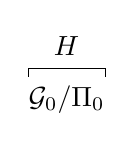
\begin{tikzpicture}[baseline=(q33.base)]
\node[inner sep=0pt] (q33) {$\mathcal{G}_0/\Pi_0$};
\draw[line width=.3pt] ([yshift=3pt]q33.north west)--([yshift=6pt]q33.north west)--([yshift=6pt]q33.north east)--([yshift=3pt]q33.north east);
\node[above=7pt] at (q33.north) {$H$};
\end{tikzpicture}\arrow[r]\arrow[d,phantom,"\simeq"{rotate=90}]
 &1\\
 &\begin{gathered}\Pi_{0\,\mathrm{ab}},\text{ noté aussi}\\\mathcal{G}^{\circ}\end{gathered}
 &&\operatorname{GL}(2,\mathbb{Z}/4\mathbb{Z})/(\dot{\ell}_0,\dot{\ell}_1)&
\end{tikzcd}}

Par générateurs et relations on a
\[
(3)\quad\mathcal{G}=\left\{\tau',\rho,\sigma\;\middle|\;
\begin{aligned}
&\rho^6=\sigma^4={\tau'}^2=1\\
&\rho^3=\sigma^2,\quad\tau'(\rho)=\rho^{-1},\quad\tau'(\sigma)=\sigma^{-1}\\
&\deleted{\unsure{\rho}}[\lambda_0,\lambda_1]=1,\quad\text{où}
\end{aligned}\right.
\]
\[
\hspace{8em}\left\{
\begin{aligned}
\lambda_0&=-\ell_0=-\sigma\rho\sigma\rho=\sigma(\rho)\rho^{\deleted{\unsure{-1|4}}}\\
\lambda_1&=-\ell_1=-\rho\sigma\rho\sigma=\rho\sigma(\rho)
\end{aligned}\right.
\]
\unsure{dont|donc} la relation de commutation $[\lambda_0,\lambda_1]=1$ s'écrit aussi
\[
(4)\qquad \sigma(\rho)\rho^2\sigma(\rho)=\rho\sigma(\rho^2)\rho
\qquad\text{ou encore}
\]
\[
(5)\qquad -\sigma\underbrace{\rho\sigma\rho^{-1}\sigma\rho}\sigma
=\underbrace{\rho\sigma\rho^{-1}\sigma\rho}
\]
où le jeu des signes $-$ peut s'expliciter dans le formalisme des gén. et rel. en supprimant dans la formule ce signe, et en remplaçant en \unsure{revanche} un (ou un \unsure{n\textsuperscript{b}|nb} impair) des $\sigma$ de la formule par des $\sigma^{-1}$. Par exemple, la formule

\margin{32}
\scanpage{34}

s'écrit, en introduisant

\margin{\uline{NB} $\lambda_\infty\overset{\mathrm{dfn}}{=}-\ell_\infty$}

\[
(6)\qquad
\lambda_\infty\deleted{\unsure{=-\ell_\infty}}
=\rho\sigma\rho^{-1}\sigma\rho
=\rho(\sigma)\sigma\rho
=-\rho\sigma(\rho)^{-1}\rho
=\rho\sigma\rho^{-1}(\sigma)
\]
sous la forme
\[
(7)\qquad [\sigma,\lambda_\infty]=1.
\]
\margin{NB $\sigma=\sigma_\infty$}

\margin{\uline{NB} On trouve
\[
\left\{
\begin{aligned}
[\ell_0,\ell_1]&=[\lambda_0,\lambda_1]=(\sigma(\rho)\rho^{-1})^3\\
[\underbrace{\sigma_{\deleted{\unsure{\infty}}}}_{\sigma}\unsure{,}\ell_\infty]
&=[\underbrace{\sigma_\infty}_{\sigma},\lambda_\infty]
=(\sigma(\rho^{-1})\rho)^3\\
&=\operatorname{int}(\sigma\rho^{-1})\cdot[\ell_0,\ell_1]
\end{aligned}\right.
\]}

On va définir un schéma en groupes \inserted{$\underline{\mathcal{G}}$} sur $\mathbb{Z}$, dont les \inserted{$\unsure{\widehat{\mathbb{Z}}|\mathbb{Z}}$-}pts seront \inserted{(à un \unsure{isom.} disons près)} les pts de $\widehat{\mathcal{G}}$. On pose
\[
(8)\qquad
\underline{M}=\underline{\mathcal{G}}^{\circ}
=\unsure{\mathbb{G}_a|\mathbb{E}_a}^{\{0,1,\infty\}}/\text{diagonale}
\]
\margin{Il vaut mieux le \unsure{noter} $\underline{M}$ --- il y a déjà trop de $\mathcal{G}$ !}

On va faire opérer \deleted{$\unsure{\mathcal{G}/M}$}
\[
\deleted{(\unsure{4})}(4)\qquad
\mathcal{G}\deleted{\unsure{=\operatorname{GL}(2,\mathbb{Z})}}
\simeq\operatorname{GL}(2,\mathbb{Z})/[\Pi_0,\Pi_0]
\]
sur $\underline{M}\deleted{\unsure{=\underline{\mathcal{G}}^{\circ}}}$,
\deleted{\unsure{en décrivant ainsi}} \inserted{à travers}
\[
(5)\qquad
\underbrace{\mathcal{G}_3\times\mu_{\unsure{\tau|2}}^{\deleted{\unsure{2}}}}_{\simeq\unsure{T_{0,3}|\Gamma_{0,3}}}
\simeq\mathcal{G}/M\deleted{\unsure{\widehat{\mathbb{Z}}}}
\simeq\mathcal{G}_{0,3}/\Pi.
\]

Désignant par $\unsure{\overbrace{\dot{\lambda}_0,\dot{\lambda}_1}},\dot{\lambda}_\infty$ les images des
$\deleted{\lambda_0,\lambda_1}\lambda_i=-\ell_i$ dans $\deleted{\unsure{M}}\mathcal{G}$, identifiées à des éléments de
\[
M=\mathcal{G}^{\circ}=\underline{\mathcal{G}}^{\circ}(\widehat{\mathbb{Z}})
\]
--- en fait on a
\[
(6)\qquad
\left\{
\begin{aligned}
\dot{\lambda}_0\unsure{,|>}\dot{\lambda}_1,\dot{\lambda}_\infty
&\in\deleted{\unsure{\underline{\mathcal{G}}^{\circ}}}\inserted{\underline{M}}(\mathbb{Z})
\subset\deleted{\unsure{\underline{\mathcal{G}}^{\circ}}}\inserted{\underline{M}}(\widehat{\mathbb{Z}})
=M\otimes_{\unsure{\cdot|\mathbb{Z}}}\unsure{\mathbb{Z}|\widehat{\mathbb{Z}}}\\
\text{donc,}\quad\dot{\lambda}_0+\dot{\lambda}_1+\dot{\lambda}_\infty&=0
\end{aligned}\right.
\]
\margin{(ici on note additivement la loi de groupe dans $M=\underline{\mathcal{G}}^{\circ}$)}

\margin{\figure{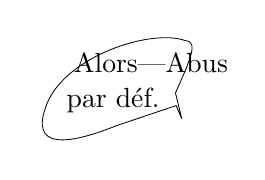
\begin{tikzpicture}[scale=.8]
\draw[line width=.3pt] (1.2,.85) .. controls (.65,1.05) and (-.7,.6) .. (-1,-.15)
 .. controls (-1.3,-.9) and (-.65,-.8) .. (.1,-.5)
 -- (1.05,-.18) -- (1.14,-.39) -- (1.04,.02)
 .. controls (1.25,.5) and (1.42,.84) .. (1.2,.85);
\node at (.65,.5) {\unsure{Alors|Abus}};
\node at (.05,-.1) {par déf.};
\end{tikzpicture}}}
$\mathcal{G}_3$ opère sur $\underline{M}=\underline{\mathcal{G}}^{\circ}$ par son action sur les \deleted{\unsure{bases}} \inserted{gén.} canoniques $\deleted{\unsure{\lambda_0}}\dot{\lambda}_0,\dot{\lambda}_1,\dot{\lambda}_\infty$, donc
\[
(7)\qquad
\left\{
\begin{aligned}
\sigma(\dot{\lambda}_0)&=\dot{\lambda}_1,\quad
\sigma(\dot{\lambda}_1)=\dot{\lambda}_0
\quad\inserted{\text{d'où}}\quad
\sigma(\dot{\lambda}_\infty)=\dot{\lambda}_\infty\\
\rho(\dot{\lambda}_i)&=\dot{\lambda}_{i+1}
\end{aligned}\right.
\]
\margin{Ceci se voit d'abord pour $i=0,1$ et, \unsure{s'en déduit} pour $i=\infty$.}
D'autre part on a par définition
\[
(8)\qquad\tau(\dot{\lambda}_i)=-\dot{\lambda}_i
\]
où
\diagram{\begin{tikzcd}[column sep=2pt,row sep=small]
\tau\arrow[d,equal]&{}={}&\sigma&\tau'\arrow[d,equal]\\
\tau_\infty&&&\tau'_\infty
\end{tikzcd}}

\margin{33}
\scanpage{35}
\mspage{665}

. L'extension $\underline{\mathcal G}$ annoncée est bien sûr celle de § 50 3°), \unsure{développé} entre-temps (depuis les premières lignes du présent §, constatant justement que j'étais gêné aux entournures pour expliciter la construction) :

(9)\quad\diagram{\begin{tikzcd}[column sep=large]
1 \arrow[r] & \underline M \arrow[r] \arrow[d,equal] & \underline{\mathcal G} \arrow[r] & H_{S_0} \arrow[r,no head] & 1 \\
 & \check V(M) & & &
\end{tikzcd}}
où $S_0=\operatorname{Spec}\mathbb Z$.

Pour $\unsure{\forall}$ schém. $S$, on posera
\[
\tag{10}
\begin{gathered}
\underline{\mathcal G}^{\Delta}(S)\subset\underline{\mathcal G}(S)\\
\Vert\;\mathrm{dfn}\\
\text{Image inverse de la ``diagonale'' de}\\
\Gamma(H_{\unsure{S|S_0}}/S)
\quad\bigl(\text{i.e. de l'image de }H\longrightarrow\Gamma(H_{\unsure{S|S_0}},S)\bigr)\\
\text{par l'hom. canonique }\underline{\unsure{\mathcal G|\mathcal E}}(S)\longrightarrow H_S(S),
\end{gathered}
\]
de sorte que par la construction du loc. cit. on aura un iso. canonique
\[
\tag{11}
\underline{\mathcal G}^{\Delta}(S)\simeq
\mathcal G\underset{M}{\wedge}\deleted{\unsure{A}}
\underbrace{\Gamma(S,\underline{\mathcal O}_S\otimes_{\mathbb Z}M)}_{
\simeq\deleted{\unsure{A}}\inserted{M}\otimes_{\mathbb Z}A\ \text{si}}
\]
et une suite exacte can.

(12)\quad\diagram{\begin{tikzcd}[column sep=large]
1 \arrow[r] & \underbrace{\Gamma(S,\underline{\mathcal O}_S\otimes_{\mathbb Z}M)}_{A\otimes_{\mathbb Z}M} \arrow[r] & \underline{\mathcal G}^{\Delta}(S) \arrow[r] & H \arrow[r] & 1.
\end{tikzcd}}

\figure{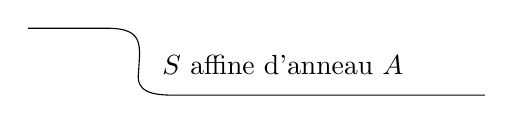
\begin{tikzpicture}[x=1cm,y=1cm]
\draw (0,0.75) -- (1.0,0.75)
.. controls (1.48,0.75) and (1.42,0.53) .. (1.40,0.18)
.. controls (1.37,-0.06) and (1.57,-0.10) .. (1.85,-0.10)
-- (5.80,-0.10);
\node[anchor=west] at (1.58,0.28) {$S$ affine d'anneau $A$};
\end{tikzpicture}}

Prenant $A=\widehat{\mathbb Z}$, on trouve en particulier (et c'est encore un fait général sur les schémas en groupes associés à des extensions de groupes discrets à noyau abélien)
\[
\tag{13}
\mathcal G^{\wedge}\simeq\underline{\mathcal G}^{\Delta}(\widehat{\mathbb Z}).
\]
\margin{34}
\scanpage{36}

2. Le groupe $\widetilde Z_{\rho,\sigma}$ : \uline{version provisoire}.

. Je vais maintenant expliciter pour $\widehat{\mathcal G}$ et $\widehat{\mathcal G}_{\unsure{0|\bullet}}\longrightarrow\widehat{\mathcal G}$ les constructions générales de § 49 $\overline{\underline{\mathrm{VI}}}$, en \inserted{y} prenant \deleted{$\unsure{\mathcal G}$}
\[
\tag{14}
\underline{\mathcal G}^{\unsure{\natural}}\overset{\mathrm{dfn}}=
\underline M=\underline{\mathcal G}^{\circ}
\quad(\text{composante neutre de }\underline{\mathcal G})
\]
Dans un cas comme celui-ci, où $\underline{\mathcal G}^{\unsure{\natural}}$ est justement le sous-groupe fermé du $(\rho,\sigma)$-groupe $\mathcal G_{\rho,\sigma}$ $(=\mathcal G^{\wedge}\text{ ici})$ engendré par $\lambda_0,\lambda_1,\lambda_\infty$, on se \unsure{dispensera} dans les notations --- là où il n'y a pas ambiguïté --- d'inclure la notation $\unsure{\natural}$. Pour \unsure{$\forall$ $A$} il y aura lieu de distinguer p.ex. entre $G_{\rho,\sigma}$ et $G_{\rho,\sigma}^{\unsure{\natural}}$ etc. \uline{Nous ferons cependant les constructions dans le cadre schématique, plutôt que profini.}

\margin{Je pense à la fin comparer les deux constructions possibles. Les \unsure{soulignés} indiqueront les \uline{schémas} en groupes...}

Le pas essentiel est de déterminer le groupe $\underline Z_{\rho,\sigma}$
\[
\tag{15}
\begin{gathered}
\underline Z_{\rho,\sigma}\subset\underline{\operatorname{Aut}}(\underline{\mathcal G}^{+})\\
\Vert\;\mathrm{dfn}\\
\left\{u\in\underline{\operatorname{Aut}}(\mathcal G^{+})\ \left|\
\begin{aligned}
\deleted{\unsure{1^{\circ}}}\ \text{a)}\;&\exists\alpha\in\underline{\mathcal G}_{\tau}^{\unsure{\natural}}=\{1,\tau\}.\underline M,
&&u(\rho)=\alpha(\rho)\\
\text{b)}\;&\exists\beta\in\text{-- -- -- -- -- --}
&&u(\sigma)=\beta(\sigma)\\
\text{c)}\;&u(L_0^{\deleted{\unsure{\Pi_0}}\mathcal G})=L_0^{\mathcal G}
&&\deleted{\unsure{(\Longleftrightarrow L_0^{\Pi_0}=L_0^{\natural})}}\\
&\qquad(\Longleftrightarrow u(L_0^{\Pi_0})=L_0^{\Pi_0})\\
\bigl[\text{d)}\;&(\text{automatique})\quad u(\mathcal G^{\unsure{\natural}})\subset\mathcal G^{\unsure{\natural}}\bigr]
\end{aligned}\right.\right.
\end{gathered}
\]

\margin{ici, ``$\exists\alpha$'' ``$\exists\beta$'' signifie bien sûr l'existence \uline{locale} de $\alpha,\beta$...}

Notons que $u$ est déterminé par les valeurs
\[
\tag{16}
\begin{cases}
u(\rho)=\xi\rho\\
u(\sigma)=\eta\sigma
\end{cases}
\qquad\xi,\eta\in\Gamma\underline\Pi
\]
\margin{où $\underline\Pi=\underline M\unsure{\rtimes}\deleted{\unsure{\{1,\tau\}}}\inserted{\unsure{\mu_2}}$ ($\underline M$ \unsure{ss-gr.|est gr.} d'indice $2$ dans $\underline\Pi$)}
\inserted{$\xi,\eta$} satisfaisant les conditions suivantes ;
\margin{35}
\scanpage{37}
\mspage{666}

\[
\tag{17}
\left\{
\begin{aligned}
\text{a)}\;&\xi\rho\ \text{(localement) conjugué à }\rho\ \text{via }\underline{\unsure{\mathcal G}}^{\unsure{\natural}}=\underline M\\
\text{b)}\;&\eta\sigma\ \text{-- -- -- -- -- -- ---}\ \sigma\ \text{'' -- -- ---}\\
\text{c)}\;&\text{équation des lacets}\\
&\xi=\eta\ell_1^{\nu}\quad\text{où }\nu\in\Gamma\mathbb G_a\ \text{convenable}\\
&\qquad\bigl(\text{tel que }\mu\overset{\mathrm{dfn}}=2\nu+1\in\Gamma\mathbb G_m\bigr)
\end{aligned}\right.
\]

. \deleted{Comme $\xi,\eta\in\Gamma N$, il faudra}

\uline{Remarque} Il n'est plus possible ici de désigner par $-1$ l'élément non trivial \inserted{$\omega$} du centre $\unsure{\mu|\mu_2}$ de $\mathcal G^{\wedge}$, et de désigner par $-x$ (pour $x\in\mathcal G^{\wedge}$) le produit de $x$ par celui-ci, à cause de la confusion avec la notation $-x$ \inserted{(pour $x\in M$)} dans le groupe abélien $M$ pour l'inverse de $x$ --- mais \deleted{\unsure{l'élém.}} $\omega x\ne-x$, puisque $\omega x\notin M$, $-x\in M$...

On pose bien sûr
\[
\tag{18}
\varepsilon_3(u)=\varepsilon_{\mathcal G}(\alpha),\qquad
\varepsilon_2(u)=\varepsilon_{\mathcal G}(\beta)
\]
(bien défini, car $\rho$ et $\rho^{-1}$ ne sont conjugués sur aucune fibre, idem pour $\sigma,\sigma^{-1}$), comment les expliciter en termes de $\xi,\eta$ ? On aura

\deleted{\unsure{(17)}}
\[
\tag{19}
\left\{
\begin{aligned}
\xi=\alpha\rho(\alpha)^{-1}
&\left\{
\begin{aligned}
&\in\Gamma\underline M\quad\text{si }\alpha\in\Gamma\underline M=\Gamma\underline{\mathcal G}^{\unsure{\natural}}\ \text{i.e. }\varepsilon_3(u)=1\\
&=\underbrace{\alpha_0}_{\in\Gamma\underline M}\tau\rho(\alpha_0\tau)^{-1}
=\alpha_0\underbrace{(-\ell_1^{-1})}_{\lambda_1^{-1}\in\underline M}\rho(\alpha_0)^{-1}\in\Gamma\underline M\quad\text{si }\varepsilon_3(u)=\unsure{-1}
\end{aligned}\right.\\[1ex]
\eta=\beta\sigma(\beta)^{-1}
&\left\{
\begin{aligned}
&\in\Gamma\underline M\quad\text{si }\beta\in\Gamma\underline M=\Gamma\underline{\mathcal G}^{\unsure{\natural}}\ \text{i.e. }\varepsilon_2(u)=1\\
&=(\underbrace{\beta_0}_{\in\Gamma\underline M}\tau)\sigma(\beta_0\tau)^{-1}
=\omega\beta_0\sigma(\beta_0)^{-1}\in\omega\underline M\quad\text{si }\varepsilon_2(u)=\unsure{-1}
\end{aligned}\right.
\end{aligned}\right.
\]
donc en tous cas
\[
\tag{19 bis}
\begin{cases}
\xi\in\Gamma\underline M\\
\eta\in\Gamma\bigl(\omega^{\nu_2(u)}.\underline{M}\bigr)
\end{cases}
\]
\margin{36}
\scanpage{38}
\mspage{676}

d'où on tire, par l'équation des lacets (17)
\[
\tag{20}
\ell_1^{\nu}=(\omega\lambda_1)^{\nu}\in\Gamma(\omega^{\nu_2(u)}.\underline M)
\quad\text{i.e. }\unsure{\Longleftrightarrow}\ \omega^{\nu}\in\Gamma(\omega^{\nu_2(u)}.\underline M)
\]
On peut l'écrire sous la forme
\[
\tag{21}
\underline\nu=2\underline\nu'+\underline\nu_2
\]
où
\[
\tag{22}
\left\{
\begin{aligned}
\underline\nu,\underline\nu' &: Z_{\rho,\sigma}\longrightarrow\mathbb G_a\\
\underline\nu_2,\underline\nu_3 &: Z_{\rho,\sigma}\rightrightarrows
(\mathbb Z/2\mathbb Z)_{S_0}^{\unsure{\mathrm{que}|\mathrm{cste}}}
\end{aligned}\right.
\]
\deleted{$\unsure{\varepsilon}$}
sont des \unsure{morphismes} de schémas bien définis, liés \inserted{entre eux et} aux hom. de groupes \deleted{$\unsure{\mu}$}
\[
\underline\mu:Z_{\rho,\sigma}\longrightarrow\mathbb G_m,\qquad
\underline\varepsilon_{\unsure{1|2}},\underline\varepsilon_3:Z_{\rho,\sigma}\longrightarrow\{\pm1\}_{S_0}
\]
par les formules (21) et
\[
\tag{23}
\left\{
\begin{aligned}
\underline\mu&=2\underline\nu\,\unsure{+}\,1\deleted{\unsure{+1}}
\quad(=4\underline\nu'\,\unsure{+}\,2\underline\nu_2+1)\\
\underline\varepsilon_2&=(-1)^{\underline\nu_2},\qquad
\underline\varepsilon_3=(-1)^{\underline\nu_3}.
\end{aligned}\right.
\]

On aura donc, en vertu de (\unsure{24|21})
\deleted{
\[
\tag{24}
\ell_1^{\nu}=\ell_1^{2\nu'}\ell_1^{\nu_2}
=\underbrace{(\omega\lambda_1)}_{\lambda_1}^{2\nu'}\ell_1^{\nu_2}
=\lambda_1^{2\nu'}\ell_1^{\nu_2}
\]
Comme $\ell_1=\lambda_1\omega$, on
\deleted{j'ai envie de mettre les $\ell_i$ sous la forme}
\[
\tag{25}
\ell_i=a_i\omega\quad\text{où }a_i\in\underline M!
\]
peut \deleted{\unsure{pour ainsi|pourra}} écrire (24) sous la forme
\[
\tag{26}
\ell_1^{\nu}=\underbrace{(\lambda_1^{\unsure{2\nu'}}a_1^{\nu_2})}_{\in\Gamma\underline M}\omega^{\nu_2}
\quad\deleted{\text{pour }\unsure{\nu_2=0|\nu_2=1}\ \text{i.e. }\unsure{\varepsilon_2=1}}
\]
Pour expliciter les $a_i$, il faut les développer en combinaisons linéaires de $\lambda_0,\lambda_1,\lambda_\infty$ (ou de deux d'entre eux, si on veut unicité).
}
\margin{37}
% ===== LM_C4-039-057: second pass, checked against the scans =====
\scanpage{39}
\mspage{667}

\[
\tag{24} l_1^\nu=\lambda_1^\nu\omega^{\nu_2}.
\]

Posant (cf (19))
\[
\tag{25}
\left\{\begin{aligned}
\beta&=\beta_0\tau^{\nu_2}\qquad(\unsure{\beta_0|\beta}\in\Gamma\underline M)\\
\eta_0&=\beta_0\sigma(\beta_0)^{-1}
\end{aligned}\right.
\]
on aura donc
\[
\eta\overset{\unsure{\mathrm{dfn}}}{=}
\beta\sigma(\beta)^{-1}
=\beta_0\sigma(\beta_0)\omega^{\nu_2}
=\eta_0\omega^{\nu_2}
\]
et l'équation du lacet prend la forme
d'une équation dans $\underline M$
\[
\tag{26}
\unsure{\zeta|\xi}=\deleted{\unsure{\beta}}\eta_0\lambda_1^\nu,
\qquad\text{i.e. \unsure{membre} de (21)}
\]
\[
\tag{26bis}\unsure{\zeta|\xi}=
\]
où $\unsure{\zeta|\xi},\eta_0$ sont deux sections de $\underline M$ qui
se déterminent mutuellement (pour $\nu$
donné). On a ainsi exprimé de façon
commode l'équation du lacet, i.e. la
condition c)\inserted{de (17)}, il reste à exprimer a) et b),
qui se formulent aussi comme
\[
\tag{27}
\left\{\begin{aligned}
\text{a)}\;&\unsure{\zeta|\xi}\ \text{localement de la forme}\quad
\overset{\inserted{(\nu_3=0)}}{\alpha_0\rho(\alpha_0)^{-1}}
\quad\text{ou}\quad
\overset{\inserted{(\nu_3=1)}}{\alpha_0\lambda_1^{-1}\rho(\alpha_0)^{-1}}\\
&\text{avec }\alpha_0\in\Gamma\underline M\\
\text{b)}\;&\eta_0\ \text{localement de la forme}\quad\beta_0\sigma(\beta_0)^{-1}
\end{aligned}\right.
\]
(Conditions dont la formulation est indépendante
de $\nu,\nu_2$ \deleted{\unsure{pour|$\nu_3$})}, mais dépend \unsure{apparemment} de
$\nu_3$.) Pour expliciter ces conditions, on
va écrire $\underline M$ additivement, les relations
s'écrivent
\margin{On a donc posé aussi $\alpha=\alpha_0\tau^{\nu_3}$}
\[
\tag{28}
\left\{\begin{aligned}
\unsure{\zeta|\xi}&=\alpha_0-\rho(\alpha_0)
\quad\overset{\inserted{\text{cas}}}{(\nu_3=0)}
\quad\text{ou}\quad
\unsure{\zeta|\xi}=\alpha_0-\rho(\alpha_0)-\lambda_1
\quad\overset{\inserted{\text{cas}}}{(\nu_3=1)}\\
\eta_0&=\beta_0-\sigma(\beta_0),
\end{aligned}\right.
\]
\margin{38}
\margin{38\\\texttt{https://grothendieck.umontpellier.fr}\\Université de Montpellier, UMR CNRS 5149, Case courrier 051, Place Eugène Bataillon\\34095 Montpellier cedex 5 - France}
\scanpage{40}

ce qu'on exprime aussi par
\[
\tag{29}
\left\{\begin{aligned}
\unsure{\zeta|\xi}&\in\operatorname{Im}(\mathrm{Id}_{\underline M}-\rho_{\underline M})
\quad(\nu_3=0)\quad\text{ou}\quad
\unsure{\zeta|\xi}\in-\lambda_1+\operatorname{Im}(\mathrm{Id}_{\underline M}-\rho_{\underline M})\\
\eta_0&\in\operatorname{Im}(\mathrm{Id}_{\underline M}-\sigma_{\underline M}).
\end{aligned}\right.
\]

C'est le moment de passer à des calculs
matriciels explicites, en rapportant $\underline M$ à
la base $\lambda_0,\lambda_1$. Dans cette base, les
\unsure{opérations} de $\rho_{\underline M},\sigma_{\underline M},\tau_{\underline M}$ sont données par
\[
\tag{30}
\left\{\begin{aligned}
\rho_{\underline M}&=\begin{pmatrix}0&-1\\1&-1\end{pmatrix}
&\mathrm{id}_{\underline M}-\rho_{\underline M}&=\begin{pmatrix}1&1\\-1&2\end{pmatrix}\\
\sigma_{\underline M}&=\begin{pmatrix}0&1\\1&0\end{pmatrix}
&\mathrm{id}_{\underline M}-\sigma_{\underline M}&=\begin{pmatrix}1&-1\\-1&1\end{pmatrix}\\
\tau_{\underline M}&=\begin{pmatrix}-1&0\\0&-1\end{pmatrix}.&&
\end{aligned}\right.
\]

On a
\[
\det(\mathrm{id}_{\underline M}-\rho_{\underline M})=3,
\qquad\det(\mathrm{id}_{\underline M}-\sigma_{\underline M})=0
\]
ce qui montre que \deleted{$\mathrm{id}_{M}$} les endomorphismes
$\mathrm{id}_{\underline M}-\rho_{\underline M}$ et $\mathrm{id}_{\underline M}-\sigma_{\underline M}$ de $\underline M$ ne sont
pas tout à fait des automorphismes\inserted{i.e. des épimorphismes} ---
Ça déconne en car. 3 pour le premier, \uline{partout}
\deleted{\unsure{car. 2}}\inserted{(en tte caractéristique)} pour le second.
\deleted{On prendra donc}\inserted{On aura}
\deleted{plus} intérêt à prendre comme "paramètres"
non $\unsure{\zeta|\xi}$ et $\eta_0$, mais bien évidemment
$\alpha_0$ et $\beta_0$ (en plus des "paramètres" discrets
$\nu_2,\nu_3$ et $\nu'$), et de \deleted{définir}\inserted{faire} \deleted{donc} un
groupe (si possible\ldots) avec les systèmes

\margin{39}
\margin{39\\\texttt{https://grothendieck.umontpellier.fr}\\Université de Montpellier, UMR CNRS 5149, Case courrier 051, Place Eugène Bataillon\\34095 Montpellier cedex 5 - France}
\scanpage{41}
\mspage{668}

\deleted{\unsure{(24)}}
\[
\tag{31}
\widetilde{\underline Z}_{\rho,\sigma}
=\left\{(\nu,\nu',\nu_2,\nu_3,\alpha_0,\beta_0)\ \left|\
\begin{gathered}
\nu,\nu'\in\Gamma\mathbf G_a,\quad
\nu_2,\nu_3\in\Gamma\{0,1\}_{S_0},\quad
\alpha_0,\beta_0\in\Gamma\underline M\\
\left\{\begin{aligned}
\unsure{\nu}&=2\nu'\unsure{-|+}\nu_2\qquad 2\nu+1\in\Gamma\mathbf G_m\\
\underbrace{\alpha_0-\rho(\alpha_0)\unsure{-|+}\nu_3\lambda_1}_{\unsure{\zeta|\xi}}
&=\underbrace{\beta_0-\sigma(\beta_0)}_{\eta}+\nu\lambda_1
\end{aligned}\right.
\end{gathered}\right.\right\}
\]
\margin{\uline{NB} $\nu'$ détermine $\nu$ qui est redondant}

L'équation des lacets, en $\alpha_0,\beta_0$, prend donc
la forme
\[
\tag{32}
(\unsure{\mathrm{id}|1}-\rho_{\underline M})\alpha_0
\unsure{-|=}(\mathrm{id}-\sigma_{\underline M})(\beta_0)
=\bigl(\underbrace{2\nu'\unsure{-|+}\nu_2}_{\nu}\unsure{+|-}\nu_3\bigr)\lambda_1
\]

\margin{Cela doit en effet \unsure{provenir du} fait que l'hom.
\diagram{\begin{tikzcd}[column sep=large]
\underline M\times\underline M\arrow[r]&\underline M\\
(\alpha_0,\beta_0)\arrow[r,mapsto]&
(\mathrm{id}-\rho_{\underline M})\alpha_0-
(\deleted{\unsure{\mathrm{id}}}\inserted{1}-\sigma_{\underline M})(\beta_0)
\end{tikzcd}}
\unsure{soit|est} bien épi\ldots\ Mais ce n'est le cas qu'en car. $\ne3$ !}

\uline{Remarque} Le schéma $\underline Z_{\rho,\sigma}$ lui $\overline{\mathrm m}$, tel qu'il
était défini au \S\ 49 \deleted{\unsure{\S\ 6}} $\overline{\underline{\mathrm{VI}}}$, n'est pas lisse
il me semble --- \unsure{ça coince|se corse} en car. 2 et 3.
Par contre le groupe $\widetilde{\underline Z}_{\rho,\sigma}$ plus fin,
défini en mettant dans le coup les
$\alpha,\beta$ tout de suite (au lieu de $(\unsure{\zeta|\xi},\eta)$)
semble bien \uline{lisse}. \unsure{Ça} amène à nouveau
à modifier un peu la présentation des
constructions du \S\ 49, en \unsure{m'interdisant|n'utilisant}
\unsure{encore un} groupe $\underline Z_{\rho,\sigma}$ (lié aux coordonnées
$\unsure{\zeta|\xi},\eta$), et en le remplaçant par
un groupe qui \unsure{apparaîtra|apparaît} \inserted{\unsure{à la fois|de façon}} comme un
normalisateur de $L_0$ (ou de $L_0^{\unsure{\sharp}}$) dans $\mathcal M_{\rho,\sigma}$
(ou $\mathcal M_{\rho,\sigma}^{\unsure{\natural|\sharp}}$). On fera une présentation dans
ce sens dans le \deleted{\unsure{suite}} \S\ suivant, et on
\unsure{suppose} ici déjà acquise cette construction,



\margin{40}
\margin{40\\\texttt{https://grothendieck.umontpellier.fr}\\Université de Montpellier, UMR CNRS 5149, Case courrier 051, Place Eugène Bataillon\\34095 Montpellier cedex 5 - France}
\scanpage{42}

D'où le \deleted{\unsure{sphère|schéma}} (schéma \deleted{et) groupe}
$\widetilde{\underline Z}_{\rho,\sigma}$ aura donc
une structure de groupe convenable, et
opère sur $\unsure{\underline C^{+}|\underline G^{+}}$ via
\[
\tag{33}
\left\{\begin{aligned}
u(\rho)&=(\alpha_0-\rho(\alpha_0)+\nu_3\lambda_1)\rho\\
u(\sigma)&=(\beta_0-\sigma(\beta_0))\omega^{\nu_2}\sigma.
\end{aligned}\right.
\]

Mais il faut quand $\overline{\mathrm m}$ vérifier que
ces formules (33) déterminent bel et
bien un automorphisme $u$ de $\unsure{\underline C^{+}|\underline G^{+}}$. La
vérification essentielle : faire en sorte
que la \deleted{formule \unsure{[7]}}\inserted{relation} (7)
\[
\tag{34}[\sigma,\lambda_\infty]
\]
est respectée par $u$.

Je vais expliciter l'action de $u$ sur
$\underline M$, en explicitant ses valeurs sur
\[
\left\{\begin{aligned}
\lambda_0&=\omega l_0=\omega\sigma\rho\sigma\rho\\
\lambda_1&=\omega l_1=\omega\rho\sigma\rho\sigma
\end{aligned}\right.
\]
en termes de \deleted{$\unsure{\zeta|\xi}$ et $\eta_0$, \unsure{intro}}
\[
\tag{35}
\left\{\begin{aligned}
\unsure{\zeta|\xi}&=\alpha_0-\rho(\alpha_0)+\nu_3\lambda_1\\
\eta_0&=\beta_0-\sigma(\beta_0)
\end{aligned}\right.
\qquad\unsure{\alpha|\&}\qquad\in\Gamma\underline M
\]
Liés à $u$ par
\[
\tag{36}
u\rho=\unsure{\zeta|\xi}\rho,\qquad
u\sigma=\omega^{\nu_2}\eta_0\sigma.
\]
On aura \deleted{donc} par la relation des lacets
\[
u(\varepsilon_0)=\deleted{\unsure{\mu}}\varepsilon_0^{\deleted{\unsure{\mu}}\inserted{(\mu)}}
\qquad(\mu=2\nu+1=4\nu'+2\nu_2+1)
\]
d'où

\margin{41}
\margin{41\\\texttt{https://grothendieck.umontpellier.fr}\\Université de Montpellier, UMR CNRS 5149, Case courrier 051, Place Eugène Bataillon\\34095 Montpellier cedex 5 - France}
\scanpage{43}
\mspage{669}
\[
u(l_0)=u(\varepsilon_0^2)=l_0^{(\mu)}
\]
et
\[
u(\lambda_0)=\unsure{u}(\omega l_0)
=\underbrace{u(\omega)}_{=\omega}\,u(l_0)
=\omega l_0^{(\mu)}
=\underbrace{\omega l_0}_{\lambda_0}
 \bigl(\underbrace{l_0^{(2\nu)}}_{\lambda_0^{2\nu}}\bigr)
=\lambda_0^{(2\nu+1)}=\lambda_0^{(\mu)}
\]
comme il convient. (Pour me rassurer, j'ai vérifié que la deuxième formule (33) donne bien
\[
u(\sigma^2)=(\eta_0\sigma)(\eta_0\sigma)
=\bigl(\underbrace{\eta_0\,\sigma(\eta_0)}_{1}\bigr)
 \deleted{\unsure{\sigma^2}}\omega=\omega
\quad\text{i.e.}\quad\deleted{\text{et}}
\]
\[
\tag{37} u(\omega)=\omega
\]
On aura
\[
u(\lambda_1)=u(\rho(\lambda_0))
=(\unsure{\zeta|\xi}\rho u)(\lambda_0)
=(\unsure{\zeta|\xi}\rho)u(\lambda_0)
=(\unsure{\zeta|\xi}\rho)(\lambda_0^\mu)=\lambda_1^\mu
\]
donc finalement, comme prédit
\[
\tag{38} u(\lambda)=\mu.\lambda\qquad\text{pour}\quad\lambda\in\Gamma\underline M
\]
\margin{où $\mu=2\nu+1=4\nu'+2\nu_2+1$}
On aura bien que $u(\sigma)=(\beta_0-\sigma(\beta_0))\omega^{\nu_2}.\sigma$
commute avec $u(\lambda_\infty)=\mu.\lambda_\infty$.

Tous ces calculs sont un peu \unsure{vaseux}, logiquement, car à la fois je veux prouver
l'existence d'un \deleted{\unsure{hom}} $u$ \inserted{de $\unsure{\underline C^{+}|\underline G^{+}}$},
et dans les calculs précédents je l'admets déjà (\unsure{implicitement}, dans un groupe
``plus gros'', savoir le schéma en groupes \unsure{lisse|libre} \inserted{(\unsure{heuristique})}
engendré par $\rho,\sigma\ldots$.
Une façon de les rendre \uline{rigoureux} serait d'utiliser la description intrinsèque de
$\unsure{\underline C^{+}|\underline G^{+}}$ :
\deleted{de \unsure{démontrer}}
\[
\tag{39}
\unsure{\underline C^{+}|\underline G^{+}}
=\unsure{C^{+}_{S_0}|G^{+}_{S_0}}
 \mathop{\wedge}_{M_{S_0}}\underline M_{S_0}
\]
donc définir un hom\inserted{$u$} de
$\unsure{\underline C^{+}|\underline G^{+}}$ dans un $S_0$-groupe $G$
(ici $G=\unsure{\underline C^{+}|\underline G^{+}}$) revient à
\margin{42}
\margin{42\\\texttt{https://grothendieck.umontpellier.fr}\\Université de Montpellier, UMR CNRS 5149, Case courrier 051, Place Eugène Bataillon\\34095 Montpellier cedex 5 - France}
\scanpage{44}
définir des homomorphismes
\[
\tag{40}
\diagram{\begin{tikzcd}[column sep=large]
\underline M_{S_0}\arrow[r,"u_{\underline M}"] & \unsure{G^{\sharp}|G^{\natural}}
\end{tikzcd}}
,\quad
\diagram{\begin{tikzcd}[column sep=large]
\unsure{C_{S_0}|G_{S_0}}\arrow[r,"u_{\unsure{C|G}}"] & \unsure{G^{\sharp}|G^{\natural}}
\end{tikzcd}}
\quad\text{i.e.}\quad
\diagram{\begin{tikzcd}[column sep=large]
\unsure{C|G}\arrow[r] & \unsure{G^{\sharp}(S_0)|G^{\natural}(S_0)}
\end{tikzcd}}
\]
satisfaisant les deux conditions suivantes :

a) Commutativité du diagramme
\[
\tag{41}
\diagram{\begin{tikzcd}[column sep=large,row sep=large]
M_{S_0}\arrow[r]\arrow[d] & \unsure{C^+_{S_0}|G^+_{S_0}}\arrow[ddr,"u_{\unsure{C|G}}"] & \\
\underline M_{S_0}\arrow[drr,"u_{\underline M}"'] & & \\
& & G
\end{tikzcd}}
\quad,
\]
et b)
\[
\tag{42}
\begin{gathered}
u_{\underline M}\text{ est compatible avec les actions}\\
\text{de }\unsure{C^+_{S_0}|G^+_{S_0}}\text{ sur }\underline M_{S_0}
\text{ (via son action sur }M_{S_0}\text{)}\\
\text{et sur }G\text{ (via }u_{\unsure{C|G}}\text{).}
\end{gathered}
\]
Dans le cas actuel, on aura $G=\unsure{\underline C|\underline G}$
\[
\tag{43}
u_{\underline M}(\lambda)=\deleted{\unsure{\lambda}}\,i(\mu.\lambda)
\]
où
\[
i:\quad
\diagram{\begin{tikzcd}[column sep=large]
\underline M\arrow[r,hook] & \unsure{\underline C^+|\underline G^+}
\end{tikzcd}}
\]
est l'inclusion, et
\[
\tag{44}
u_{\unsure{C|G}}:\deleted{\text{défini par}}
\inserted{\diagram{\begin{tikzcd}[column sep=large]
\unsure{C^+_{S_0}|G^+_{S_0}}\arrow[r]&G
\end{tikzcd}}}
\qquad\text{défini par (33),}
\]
Il faut donc d'abord vérifier que (33), définit bien un hom
\diagram{\begin{tikzcd}[column sep=small]\unsure{C_{S_0}|G_{S_0}}\arrow[r]&G\end{tikzcd}},
ou ce qui revient au $\overline{\mathrm m}$,
\diagram{\begin{tikzcd}[column sep=small]\unsure{C|G}\arrow[r]&G(S_0)\end{tikzcd}}.
\margin{43}
\margin{43\\\texttt{https://grothendieck.umontpellier.fr}\\Université de Montpellier, UMR CNRS 5149, Case courrier 051, Place Eugène Bataillon\\34095 Montpellier cedex 5 - France}
\scanpage{45}
\mspage{\textcircled{670}}
Pour cela on \deleted{\unsure{note que} $u$ définit un hom \unsure{au} \unsure{d'indice} de $3$
$\unsure{C|G}$}
\inserted{utilise la présentation \deleted{\unsure{de}} de $\unsure{C^+|G^+}$}
\[
\deleted{\begin{gathered}
\unsure{C_0^+|G_0^+}\\
\unsure{\simeq}\\
\unsure{\operatorname{SL}(2,\mathbb Z)}=
\{\rho,\sigma\mid\rho^6=\sigma^4=1\}
\end{gathered}}
\]
\[
\tag{44}
\unsure{C^+|G^+}=
\left\{\rho,\sigma\ \middle|\ 
\begin{gathered}
\rho^6=\sigma^4=1,\quad\rho^3=\sigma^2\\
[\sigma,\lambda_\infty]=1\quad\text{où}\quad
\lambda_\infty=\deleted{\unsure{\rho}}\rho\sigma\rho^{-1}\sigma\rho
\end{gathered}
\right\},
\]
donc posant
\[
\tag{45}
\left\{\begin{aligned}
\rho'&=\unsure{\zeta\rho|u(\rho)},\quad
\sigma'=\eta_0\omega^{\nu_2}\sigma\qquad\text{cf (33) et}\\
\unsure{\zeta|\xi}&=\alpha_0-\rho(\alpha_0)+\nu_3\lambda_1,\quad
\unsure{\eta|\eta_0}=\beta_0-\sigma(\beta_0)
\end{aligned}\right.
\]
il faut vérifier les relations
\[
\tag{46}
\rho'{}^6=\sigma'{}^4=[\sigma',\lambda'_\infty]=1,\quad
\rho'{}^3=\sigma'{}^2
\quad\text{où}\quad
\lambda'_\infty=\deleted{\unsure{\rho'(\lambda'_0)}}
\inserted{\rho'\sigma'\rho'{}^{-1}\sigma'\rho'}.
\]
On commencera par vérifier \deleted{\unsure{que|plus}}
\[
\tag{47}\rho'{}^3=\sigma'{}^2=\omega
\]
ce qui implique \deleted{\unsure{que}}
\[
\tag{48}
\rho'{}^6=\sigma'{}^4=1,\quad\text{donc}\quad
\exists\ \deleted{\text{unique}}
\diagram{\begin{tikzcd}[column sep=large]
\unsure{C_0^+|G_0^+}\arrow[r,"u_{\unsure{C_0|G_0}}"] & G(S_0)\\
\rho\arrow[r,mapsto]&\rho',\quad\sigma\mapsto\sigma'
\end{tikzcd}}
\]
Ensuite, \deleted{posant} notant qu'on aura
\[
\lambda'_\infty=u_{\unsure{C_0|G_0}}(\lambda_\infty),
\]
il suffira de \deleted{\unsure{cela}} vérifier
\[
\tag{49}\lambda'_\infty=\mu\lambda_\infty
\]
il sera évident que $\lambda'_\infty$ commute à
\[
\sigma'=u(\sigma)=\eta_0\sigma\qquad\deleted{\text{\unsure{pui}}}
\]
puisque $\sigma$ et $\eta_0\in M$ y commutent. Donc pour construire
$u_{\unsure{C|G}}$, les vérifications essentielles sont (47) et (49)
--- d'ailleurs une fois (47) prouvé, les calculs précédents aboutissant à (38)
sont justifiés (\unsure{au moins} là où ils ont un sens, i.e.,
pour $u_{\unsure{C|G}}$ et $\lambda\in M$),
\margin{44}
\margin{44\\\texttt{https://grothendieck.umontpellier.fr}\\Université de Montpellier, UMR CNRS 5149, Case courrier 051, Place Eugène Bataillon\\34095 Montpellier cedex 5 - France}
\scanpage{46}
donc (49) sera bien vérifié.

On \deleted{aura} a
\[
\begin{aligned}
&\deleted{\unsure{u(\rho)=}}\\
\rho'{}^3&=\bigl(\unsure{\zeta|\xi}\rho(\unsure{\zeta|\xi})\rho^2(\unsure{\zeta|\xi})\bigr)\rho^3
=\unsure{\zeta|\xi}\rho(\unsure{\zeta|\xi})\rho^2(\unsure{\zeta|\xi})\,\omega\\
\sigma'{}^2&=(\eta_0\sigma(\eta_0))\sigma^2=(\eta_0\sigma(\eta_0))\omega
\end{aligned}
\]
donc \deleted{et} les formules (47) se réduisent à :
\[
\tag{50}
\unsure{\zeta|\xi}\rho(\unsure{\zeta|\xi})\rho^2(\unsure{\zeta|\xi})=1,
\qquad\eta_0\sigma(\eta_0)=1
\]
soit, additivement
\[
\unsure{\zeta|\xi}+\rho(\unsure{\zeta|\xi})+\rho^2(\unsure{\zeta|\xi})=0,
\qquad\eta_0+\sigma(\eta_0)=0.
\]
dont la vérification est triviale, compte tenu que
\[
\rho_{\underline M}^3=\sigma_{\underline M}^2=\mathrm{id}_{\underline M},
\qquad(1+\rho_{\underline M}+\rho_{\underline M}^2)
=\deleted{\unsure{\mathrm{id}_{\underline M}}}0_{\underline M}.
\]
On a donc bien construit un hom
\deleted{\unsure{au}}
\[
u_{\unsure{C_0^+|G_0^+}}:\quad
\diagram{\begin{tikzcd}[column sep=large]
\unsure{C_0^+|G_0^+}\arrow[r]&\unsure{\underline C_0^+(S_0)|\underline G_0^+(S_0)}
\end{tikzcd}},
\]
et il reste à vérifier (41) et (42).

Pour (41), nous l'avons déjà montré au \inserted{niveau de l'existence d'un $u_{\unsure{C_0|G_0}}$}
--- elle revient à prouver
\[
\bigl(\quad u_{\unsure{C_0|G_0}}(\lambda_0)=\deleted{\unsure{\lambda_0}}\mu\lambda_0,
\quad u_{\unsure{C_0|G_0}}(\lambda_1)=\mu\lambda_1
\]
Je vais quand $\overline{\mathrm m}$ refaire la vérification, pour être sûr.
\[
\begin{aligned}
\varepsilon'_0&=u_{\unsure{C_0|G_0}}(\underbrace{\varepsilon_0}_{\sigma\rho})
=u_{\unsure{C_0|G_0}}(\sigma)u_{\unsure{C_0|G_0}}(\rho)
=\eta_0\omega^{\nu_2}\deleted{\unsure{\zeta|\xi}}\sigma\unsure{\zeta|\xi}\rho
=\eta_0\omega^{\nu_2}\sigma(\unsure{\zeta|\xi})\sigma\rho\\
&=\eta_0\sigma(\unsure{\zeta|\xi})\omega^{\nu_2}\varepsilon_0
\end{aligned}
\]
\margin{45}
\margin{45\\\texttt{https://grothendieck.umontpellier.fr}\\Université de Montpellier, UMR CNRS 5149, Case courrier 051, Place Eugène Bataillon\\34095 Montpellier cedex 5 - France}
\scanpage{47}
\mspage{\unsure{671}}

Je dis que
\[
\begin{aligned}
\varepsilon'_0&=\varepsilon_0^{(\mu)}\quad\text{i.e.}\quad
\eta_0\sigma(\unsure{\zeta|\xi})\omega^{(\nu_2)}
 =\underbrace{\varepsilon_0^{(\mu-1)}}_{l_0^\nu}
\quad\text{où }\mu-1=2\nu\deleted{\unsure{+1|=1}},\quad\text{soit}\\
\eta_0\sigma(\unsure{\zeta|\xi})\omega^{\nu_2}&=l_0^{(\nu)}
\quad\text{où }\nu=2\nu'\unsure{-|+}\nu_2\quad\text{i.e.}\\
\eta_0\sigma(\unsure{\zeta|\xi})
 &=\underbrace{l_0^{(2\nu')}}_{\lambda_0^{2\nu'}}
 \underbrace{\unsure{(\omega l_0)^{(-\nu_2)}|(\omega l_0^{(-\nu_2)})}}_{\lambda_0^{-\nu_2}}
 =\underbrace{\lambda_0^{(2\nu'\unsure{-|+}\nu_2)}}_{\lambda_0^\nu}
 \quad\text{i.e.}\\
\eta_0\sigma(\unsure{\zeta|\xi})&=\lambda_0^{(\nu)}
\end{aligned}
\]
soit, en appliquant $\sigma$ et notant que
$\sigma(\eta_0)=\eta_0^{-1}$, $\sigma^2(\unsure{\zeta|\xi})=\unsure{\zeta|\xi}$,
$\sigma(\lambda_0)=\lambda_1$,
\[
\eta_0^{-1}\unsure{\zeta|\xi}=\lambda_1(\nu)
\quad\text{soit enfin }\deleted{\unsure{\zeta_0=|\xi_0=}}
\unsure{\zeta|\xi}=\eta_0\unsure{\lambda_1(\nu)|\lambda_1^{(\nu)}}
\quad\text{ou}
\]
\[
\unsure{\zeta|\xi}=\eta_0+\nu\lambda_1\quad\text{(écrit additivement)}
\]
ce qui est vrai par hypothèse (cf (31)).

On aura ensuite
(\deleted{\unsure{pour $u=u_{\unsure{C_0|G_0}}$|pour $u_{\unsure{C_0|G_0}}$}}
\inserted{écrivant $u$ au lieu de $u_{\unsure{C_0|G_0}}$ pour simplifier})
\[
u_{\deleted{\unsure{C_0|G_0}}}(\lambda_1)
 =u\rho(\lambda_0)
 =(\unsure{\zeta|\xi}\rho u)(\lambda_0)
 =\unsure{\zeta|\xi}\rho(u(\lambda_0))
 =\unsure{\zeta|\xi}\rho(\lambda_0(\mu))
 =\lambda_1(\mu)
\]
OK.

Reste à vérifier (42), ce qui \deleted{\unsure{signifie}}
\inserted{revient} à la \unsure{commutativité} de
$u_{\underline M}=\mu\,\mathrm{id}_{\underline M}$ à
$(\rho_{\underline M},\rho'_{\underline M})$,
$(\sigma_{\underline M},\sigma'_{\underline M})$
--- \unsure{ce signifie} aussi que
$\rho_{\underline M}$ et $\rho'_{\underline M}$ d'une part,
$\sigma_{\underline M}$ et $\sigma'_{\underline M}$ d'autre part,
\deleted{\illegible{2}}\inserted{sont égaux, ce}
qui est également évident.

Ainsi, le groupe $\widetilde Z_{\rho,\sigma}$ est bel et
bien construit --- du moins, en tant que
schéma sur $S_0=\mathrm{Spec}\,\mathbb Z$, avec des morphismes
de schémas
\[
\tag{51}
\diagram{$
\begin{tikzcd}[column sep=3em,row sep=.25em]
\widetilde{\underline Z}_{\rho,\sigma}\arrow[r,"\nu'"] & G_a\\
{}\arrow[r,"\deleted{\unsure{\nu|\varepsilon}}"] & \deleted{\unsure{\{\pm1\}_{S_0}^{2}|\mu_{S_0}^{2}}}\\
{}\arrow[r,"\nu_2"] & \{0,1\}_{S_0}\\
{}\arrow[r,"\nu_3"] & \{0,1\}_{S_0}
\end{tikzcd}
\quad\Bigg|\quad
\begin{gathered}
\text{d'où }\mu=4\nu'+2+\nu_2:\quad
\begin{tikzcd}[column sep=1.5em,row sep=1em]
\widetilde Z_{\rho,\sigma}\arrow[r]\arrow[rd] & G_a\\
 & G_m\arrow[u,hook]
\end{tikzcd}\\
\varepsilon_2,\varepsilon_3:\quad
\begin{tikzcd}[column sep=3em]
\widetilde Z_{\rho,\sigma}\arrow[r,shift left=.3ex]\arrow[r,shift right=.3ex]
 & \mu_{S_0}=\{\pm1\}_{S_0}
\end{tikzcd}
\end{gathered}
$}
\]

\margin{46}
\margin{46\\\texttt{https://grothendieck.umontpellier.fr}\\Université de Montpellier, UMR CNRS 5149, Case courrier 051, Place Eugène Bataillon\\34095 Montpellier cedex 5 - France}
\scanpage{48}

et un morphisme de \deleted{\unsure{foncteurs}} \inserted{préfaisceaux} sur $S_0$
\[
(52)\qquad
\diagram{\begin{tikzcd}[row sep=small]
\widetilde{\underline Z}_{\rho,\sigma} \arrow[r] & \underline{\operatorname{Aut}}_{\mathrm{gr}}\bigl(\unsure{\underline C^{+}|\underline G^{+}}\bigr),\\
\underline u \arrow[r,mapsto] & u
\end{tikzcd}}
\]
donnant lieu à un morphisme
\[
(53)\qquad
\diagram{\begin{tikzcd}[row sep=small]
\widetilde{\underline Z}_{\rho,\sigma} \arrow[r] & \underline{\operatorname{Aut}}_{\mathrm{gr}}\bigl(\unsure{\underline C^{+}|\underline G^{+}}\bigr)\times\mathbf G_{\mathrm m}\times\mu_{S_0}\times\mu_{S_0}\\
\underline u \arrow[r,mapsto] & u,\mu(\underline u),\varepsilon_2(\underline u),\varepsilon_3(\underline u)
\end{tikzcd}}
\]
--- des calculs déjà faits trente six fois dans des contextes divers doivent montrer que ce morphisme (qui est \uline{mono.}\ \unsure{?}\ en car. $\ne 2,3$) est un morphisme de \uline{groupes}, pour une structure de \uline{\unsure{groupe|groupes}} convenable sur $\widetilde{\underline Z}_{\rho,\sigma}$, uniquement déterminée (car elle l'est en car. $\ne 2,3$, et on conclut par raison de densité schématique). On aura \deleted{\unsure{ce n'est pas}}
\[
(54)\qquad
\diagram{\begin{tikzcd}
1\arrow[r]&\widetilde{\underline Z}_{\rho,\sigma}^{+0}\arrow[r]&\widetilde{\underline Z}_{\rho,\sigma}\arrow[r]&\mathbf G_{\mathrm m}\times\mu_{S_0}\times\mu_{S_0}\arrow[r]&1
\end{tikzcd}}
\]
\margin{un peu \unsure{cavalier}, car
\diagram{\begin{tikzcd}
\underline Z_{\rho,\sigma}\arrow[r]&\mathbf G_{\mathrm m}\times\mu_{S_0}\times\mu_{S_0}
\end{tikzcd}}
n'est pas un épi, du fait que
\diagram{\begin{tikzcd}[row sep=small]
\underline M\times\underline M\arrow[r]&\underline M\\
(\alpha_0,\beta_0)\arrow[r,mapsto]&(1-\rho_{\underline M})\alpha_0\unsure{-|+}(1-\sigma_{\underline M})\beta_0
\end{tikzcd}}
n'est pas épi --- \unsure{où il} y a \unsure{canular} en car. 3 --- cf plus bas\ldots}
en explicitant
\[
(55)\qquad
\begin{gathered}
\widetilde{\underline Z}_{\rho,\sigma}^{+0}\underset{\inserted{\text{sous-schéma en groupes}}}{\subset}\underline M\times\underline M\times\mathbf G_{\mathrm a}\\
\Vert\\
\left\{(\alpha_0,\beta_0,\nu')\,\middle|\,
\begin{gathered}
\deleted{\unsure{\alpha_0}}4\nu'=0\\
(1+\rho_{\underline M})\alpha_0=(1-\sigma_{\underline M})\beta_0+2\nu'\lambda_1
\end{gathered}\right\}
\end{gathered}
\]
On aura donc
\[
(56)\qquad
\diagram{\begin{tikzcd}
1\arrow[r]&\widetilde{\underline Z}_{\rho,\sigma}^{+00}\arrow[r]&\widetilde{\underline Z}_{\rho,\sigma}^{+0}\arrow[r]&\underline{{}_4\mathbf G_{\mathrm a}}\arrow[r]&1
\end{tikzcd}}
\]
\margin{47}
\margin{47\\\texttt{https://grothendieck.umontpellier.fr}\\Université de Montpellier, UMR CNRS 5149, Case courrier 051, Place Eugène Bataillon\\34095 Montpellier cedex 5 - France}
\scanpage{49}
\mspage{672}

où
\[
(57)\qquad
\begin{gathered}
\widetilde{\underline Z}_{\rho,\sigma}^{+00}\overset{\mathrm{dfn}}{=}
\left\{\underline u\in\Gamma\widetilde{\underline Z}_{\rho,\sigma}\,\middle|\,
\nu'(\underline u)=\nu_2(\underline u)=\nu_3(\unsure{u|\underline u})=0\right\}\\
\simeq\\
\left\{(\alpha_0,\beta_0)\in\Gamma(\underline M\times\underline M)\,\middle|\,
(1-\rho_{\underline M})\alpha_0=(1-\sigma_{\underline M})\beta_0\right\}.
\end{gathered}
\]
\margin{en car. 3 sa dimension relative \unsure{saute} de 2 à 3 !}
schéma en \uline{groupes} $\underline Z_{\rho,\sigma}^{+00}$ est lisse \inserted{en car. $\ne 3$} de dim relative 2 --- c'est $\overline{\mathrm m}$ de façon canonique un schéma en Modules, on aura
\[
(58)\qquad\widetilde{\underline Z}_{\rho,\sigma}^{+00}\simeq\unsure{\mathbf V|\mathbb V}(\underline P)
\]
où $P$ est le $\mathbb Z$-module libre de rang 2 défini \deleted{\illegible{1}} par la suite exacte
\[
(59)\qquad
\diagram{\begin{tikzcd}[row sep=small]
0\arrow[r]&\deleted{\unsure{M}}\inserted{P}\arrow[r]&M\times M\arrow[r]&M\arrow[r]&0\\
&&(\alpha_0,\beta_0)\arrow[r,mapsto]&(1-\rho_{\underline M})\alpha_0-(1-\sigma_{\underline M})\beta_0&
\end{tikzcd}}
\]
L'hom $M\times M\longrightarrow M$ s'explicite, en posant
\[
(60)\qquad
\left\{\begin{aligned}
\alpha_0&=a_0\lambda_0+\unsure{a_1}\lambda_1
&\text{d'où}\quad\alpha_0-\rho\alpha_0&=(a_0+\unsure{a_1})\lambda_0+(2\unsure{a_1|b_1}-a_0)\lambda_1\\
\beta_0&=b_0\lambda_0+b_1\lambda_1
&\text{d'où}\quad\beta_0-\sigma\beta_0&=(b_0-b_1)\lambda_0+(b_1-b_0)\lambda_1
\end{aligned}\right.
\]
comme
\[
(61)\qquad
\diagram{\begin{tikzcd}
(\alpha_0,\beta_0)\arrow[r,mapsto]&
\underbrace{(a_0+a_1+(b_1\unsure{-|+}b_0))}_{c_0}\lambda_0+
\underbrace{(2a_1-a_0-(b_1-b_0))}_{c_1}\lambda_1
\end{tikzcd}}
\]
\deleted{\unsure{On}} C'est un hom surjectif \inserted{sauf en car. 3}, \deleted{pour $(c_0,c_1)$ donnés,}
\deleted{\unsure{on fera}\ $\unsure{a_1|c_1}$\ \illegible{1}}
\inserted{--- les éléments de l'image sont les}
\[
(62)\qquad
\left\{c_0\lambda_0+c_1\lambda_1\,\middle|\,
\underbrace{c_0+c_1}_{=3a_1}\equiv0\quad(3)\right\}
\]
\uline{Remarque} Si on prend \deleted{\unsure{un}}\inserted{un} $u$ défini sur $\widehat{\mathbb Z}$ provenant d'un élément de $M[0]$, alors
\margin{48}
\margin{48\\\texttt{https://grothendieck.umontpellier.fr}\\Université de Montpellier, UMR CNRS 5149, Case courrier 051, Place Eugène Bataillon\\34095 Montpellier cedex 5 - France}
\scanpage{50}

on aura \deleted{que}
\[
\mu\in\widehat{\mathbb Z}^{*},\quad
\mu\equiv\deleted{\unsure{\varepsilon_3|\varepsilon_2}}(-1)^{\nu_3}(=1-2\nu_3)\quad\mathrm{mod}\ (3)
\]
et la condition sur $(\mu,\varepsilon_2,\varepsilon_3)$ pour être dans l'image de
\[
\diagram{\begin{tikzcd}
\widetilde{\underline Z}_{\rho,\sigma}\arrow[r]&\mathbf G_{\mathrm m}\times\mu_{S_0}\times\mu_{S_0}
\end{tikzcd}},
\]
qui s'écrit en général (en vertu de (62) \unsure{\&} et de (32))
\[
2\nu'-\nu_2+\nu_3\equiv0\quad(3)
\]
devient, en multipliant par 2
\[
\underbrace{4\nu'-2\nu_2}_{\mu-1}+2\nu_3\equiv0\quad(3)
\]
i.e
\[
\mu\equiv1-2\nu_3\quad(3),
\]
et elle est automatiquement satisfaite.

\deleted{
C'est pourquoi j'ai envie de modifier la définition de \deleted{$\unsure{Z}$} $\widetilde{\underline Z}_{\rho,\sigma}$, en définissant $\underline Z_{\rho,\sigma}$ comme
\[
\deleted{(63)\quad\widetilde{\underline Z}_{\rho,\sigma}=}
\left\{\begin{gathered}
\deleted{\unsure{\Gamma|\mu}}(\inserted{\mu,}\nu',\nu'',\nu_2,\nu_3,\alpha_0,\beta_0)
\in\mathbf G_{\mathrm m}\times\mathbf G_{\mathrm a}\times\unsure{\mathbf G_{\mathrm a}}\times\{0,1\}_{S_0}\times\{0,1\}_{S_0}\times\underline M\times\underline M\\
\left|\begin{gathered}
\mu=4\nu'\unsure{-|+}2\unsure{\nu_2}+1(=6\nu''-2\nu_3+1),\quad 2\nu'+\nu_3-\nu_2=3\nu'',\\
(\unsure{1}-\rho_{\underline M})(\alpha_0)-(1-\sigma_{\underline M})(\beta_0)
=\underbrace{(\deleted{\unsure{2\nu'-\nu_2+\nu_3}}\inserted{3\nu''})}_{c}\lambda_1
\end{gathered}\right.
\end{gathered}\right\}
\]
}
\margin{en \unsure{exprimant|exigeant} $\unsure{\mu|\nu}$\ \unsure{s'écrivent}
\[
\begin{aligned}
\mu&\equiv1-2\nu_2\quad(4)\\
\mu&\equiv1-2\nu_3\quad(6)
\end{aligned}
\unsure{\left[\vphantom{\begin{matrix}\mu\\\mu\end{matrix}}\right.}
\]
\deleted{l'équation des lacets}
\[
\begin{aligned}
\mu&=1\unsure{-|+}2\nu_2+4\nu'&&\text{\unsure{avec}}\\
\mu&=1-2\nu_3+6\nu''\\
-\nu_2+2\nu'&=-\nu_3+3\nu''&&\text{i.e.}\\
2\nu'+\nu_3-\nu_2&=3\nu''
\end{aligned}
\]}
\deleted{
\deleted{On aura ici
\[
2c=6\nu'',\quad\text{et on \unsure{va|a} en fait}
\]
prendre $c=3\nu''$, et.}
On aura
\[
(63)\qquad
\begin{gathered}
\widetilde{\underline Z}_{\rho,\sigma}\subset\mathbf G_{\mathrm a}\times\mathbf G_{\mathrm a}\times\{0,1\}_{S_0}\times\{0,1\}_{S_0}\times\underline M\times\underline M\\
\Vert\\
\left\{(\nu',\nu'',\nu_2,\nu_3,\alpha_0,\beta_0)\,\middle|\,
\begin{aligned}
\text{a)}\quad &2\nu'\deleted{+\unsure{\nu_3}}-\nu_2=3\nu''-\nu_3\\
&\deleted{(\text{d'où }4\nu'\unsure{-|+}2\nu_2+1=6\nu''-2\nu_3+1,\ \text{soit }\mu)}\\
&\inserted{\text{soit }\nu,\ \text{d'où }\mu=2\nu+1}\\
\text{b)}\quad &\mu\in\Gamma\mathbf G_{\mathrm m}\\
\text{c)}\quad &\text{équation des \unsure{lacets|lacet}}\\
&(1-\rho_{\underline M})(\alpha_0)-(1-\sigma_{\underline M})(\beta_0)=3\nu''\unsure{\underline{\lambda_1}|\lambda_1}
\end{aligned}\right\}
\end{gathered}
\]
}
\margin{49}
\margin{49\\\texttt{https://grothendieck.umontpellier.fr}\\Université de Montpellier, UMR CNRS 5149, Case courrier 051, Place Eugène Bataillon\\34095 Montpellier cedex 5 - France}
\scanpage{51}
\mspage{673}

3. Les groupes \deleted{$\unsure{\widetilde Z_{\rho,\sigma}}$ \unsure{révisés} \illegible{2} $\mathbb O_N$} $\mathbb O_N^{*}$.

On va introduire une construction auxiliaire,
en définissant un schéma en groupes qui
correspond à la donnée de quantités
$\mu\in\Gamma\mathbf G_{\mathrm m}$, $\nu',\nu''\in\Gamma\mathbf G_{\mathrm a}$,
$\nu_2,\nu_3\in\Gamma\{0,1\}_{S_0}$, satisfai-
sant
\[
(63)\qquad
\mu=4\nu'-2\nu_2+1=6\nu''-2\nu_3+1,
\qquad 2\nu'-\nu_2=3\nu''-\nu_3.
\]

De façon générale, soit $N$\inserted{$\in\mathbb N^{*}$} un entier \inserted{naturel} fixé
(le cas qui nous intéresse pour la suite est
$N=12$), et considérons le schéma \inserted{en groupes, $\mathbb O_N$}
sur $\mathbb Z$ associé à l'extension de groupes discrets
\deleted{\[(64)\qquad \mathbb O_N\]}
\[
(64)\qquad
\diagram{\begin{tikzcd}[column sep=large]
1\arrow[r]&\mathbb Z\arrow[r,"N"]&\mathbb Z\arrow[r]&\mathbb Z/N\mathbb Z\arrow[r]&1
\end{tikzcd}}
\]
qui s'insère dans une suite exacte
\[
(65)\qquad
\diagram{\begin{tikzcd}[column sep=large]
1\arrow[r]&\unsure{\mathbf E^{1}|\mathbb E^{1}}\arrow[r,"i"]&\mathbb O_N\arrow[r]&(\mathbb Z/N\mathbb Z)_{S_0}\arrow[r]&1.
\end{tikzcd}}
\]

Rappelons la \deleted{\unsure{défi}} construction simple
\[
(66)\qquad
\mathbb O_N
=(\mathbb Z)_{S_0}\mathop{\wedge}_{(N\mathbb Z)}\underline{N\mathbb Z}.
\]
\deleted{Mais} Je dis qu'il y a \unsure{dans|sur} $\mathbb O_N$ une
structure d'Anneaux unique, dont l'
addition soit la structure de groupe \inserted{abélien} déjà
envisagée, et où la multiplication est
obtenue ainsi : Une section de $\mathbb O_N$ est
\deleted{locale} de la forme \deleted{$\unsure{k|x}$} $n+N[\lambda]$, avec
les règles de calcul
\[
(67)\qquad
\left\{\begin{aligned}
\text{a)}\quad &(n+N[\lambda])+(n'+N[\lambda'])=(n+n')+N[\lambda+\lambda']\\
\text{b)}\quad &n+N[\lambda]=n'+N[\lambda']\Longleftrightarrow
\deleted{\unsure{\xi|n}}\ n+N\lambda=n'+N\lambda'\text{ dans }\Gamma\mathbf G_{\mathrm a}.
\end{aligned}\right.
\]

\margin{50}
\margin{50\\\texttt{https://grothendieck.umontpellier.fr}\\Université de Montpellier, UMR CNRS 5149, Case courrier 051, Place Eugène Bataillon\\34095 Montpellier cedex 5 - France}
\scanpage{52}

On multiplie alors les sections par
\[
(68)\qquad
(\unsure{n}+N[\lambda])(n'+N[\lambda'])
=nn'+N[n\lambda'+n'\lambda+\lambda\lambda'],
\]
on vérifie que c'est \deleted{\unsure{biad}} compatible aux
relations (67 b), que c'est biadditif,
commutatif, associatif, que $1+N[0]$ est
unité\ldots{} Autre façon de \deleted{\unsure{la|le} \unsure{con|en}} voir la
structure d'anneaux. \deleted{On} Soit plus
généralement \deleted{$\mathbb O_N=\mathbb Z_{S_0}$}
$A$ une \deleted{$\unsure{\mathbb Z|z}$} $\mathbb Z$-algèbre
\deleted{\unsure{com}} associative \inserted{\unsure{unifère|unitaire}} (disons)
\deleted{\unsure{principal}} \inserted{munie d'un \uline{idéal}}
\margin{\inserted{bilatère}} $J$ \inserted{qui soit}
un $\mathbb Z$-module libre de t.f., considérons
\deleted{\unsure{un} idéal}
\deleted{l'idéal $NA$} et la structure d'
extension
\[
(69)\qquad
\diagram{\begin{tikzcd}[column sep=large]
0\arrow[r]&\deleted{\unsure{NA}}\inserted{J}\arrow[r]&A\arrow[r]&\overbrace{A/\deleted{\unsure{NA|N}}\inserted{J}}^{B}\arrow[r]&0
\end{tikzcd}}
\]
d'où un schéma en groupes commu-
tatif $\underline A_{[N]}$, qui s'obtient comme
quotient de
\deleted{$(A)_{\unsure{S|S_0}}\cdot\underline{\unsure{NB|NA}}\;\unsure{\xi\to|p}$}
\inserted{$A_{S_0}\cdot\underline J$ produit}
semi-direct)
\[
(70)\qquad
\diagram{\begin{tikzcd}[column sep=large]
0\arrow[r]&\underline J\arrow[r]&A_{S_0}\times\underline J\arrow[r]&\underline A_N\arrow[r]&0\\
&\lambda\arrow[r,mapsto]&(\lambda,-\lambda)&&
\end{tikzcd}}
\]
et on trouve que $A_{S_0}\cdot\underline J$ a une structure
\uline{d'Anneaux} produit $\frac12$-direct, et que

\margin{51}
\margin{51\\\texttt{https://grothendieck.umontpellier.fr}\\Université de Montpellier, UMR CNRS 5149, Case courrier 051, Place Eugène Bataillon\\34095 Montpellier cedex 5 - France}
\scanpage{53}
\mspage{674}

l'image de $\underline J$ y est un idéal ...

On trouve bien une structure d'anneau sur $\underline A_{[N]}$, et une suite exacte \deleted{\unsure{de}}
\[
\tag{71}
\diagram{\begin{tikzcd}[column sep=large]
1 \arrow[r,no head] & \underline J \arrow[r,no head] & \underline A_{[N]} \arrow[r] & B_{S_0} \arrow[r] & 1
\end{tikzcd}}
\]
où $\underline A_{[N]}\mathbin{-}B_{S_0}$ est un \unsure{hom.} de \uline{schémas en anneaux}. Passant aux groupes \deleted{\unsure{anneaux}} multiplicatifs, on trouve une suite exacte
\[
\tag{72}
\diagram{\begin{tikzcd}[column sep=large,row sep=small]
1 \arrow[r] & (1+\underline J)^* \arrow[r,no head] & A_{[N]}^* \arrow[r,no head] & (B_{S_0})^* \arrow[r,no head] \arrow[d,equal] & 1 \\
& & & (B^*)_{S_0} &
\end{tikzcd}}
\]
où pour $A_{[N]}^*$, $(B_{S_0})^{\unsure{*|'}}$ et $B^*$, le $*$ désigne le \unsure{passage} au \unsure{s-groupe} multiplicatif et où $(1+\underline J)^*$ a le sens analogue
\[
\tag{73}
\diagram{\begin{tikzcd}[row sep=large]
(1+\underline J)^*\unsure{\subset|\subseteq}1+\underline J \arrow[d,draw=none,"="{description,rotate=90}] \\
\{(1+\lambda)\mid 1+\lambda\ \text{inv. dans }\underline A\} \arrow[d,draw=none,"\simeq"{description,rotate=90}] \\
\{(\lambda,\lambda')\in\underline J\times\underline J\mid\lambda+\lambda'+\lambda\lambda'=0\ \text{dans }\underline J\}.
\end{tikzcd}}
\]

Ainsi on aura, dans le cas particulier $A=\mathbb Z$, $J=N\mathbb Z$
\[
\tag{74}
\diagram{\begin{tikzcd}[column sep=large]
1 \arrow[r] & (\underline{1+N\mathbb Z})^* \arrow[r] & \mathbb O_N^* \arrow[r,no head] & (\mathbb Z/N\mathbb Z)^*_{S_0} \arrow[r,no head] & 1
\end{tikzcd}}
\]
où le noyau

\margin{52}
\margin{52\\\texttt{https://grothendieck.umontpellier.fr}\\Université de Montpellier, UMR CNRS 5149, Case courrier 051, Place Eugène Bataillon\\34095 Montpellier cedex 5 - France}
\scanpage{54}
\deleted{\mspage{\unsure{674}}}

$(1+N\mathbb Z)^*$ est défini comme
\[
\tag{75}
(1+N\mathbb Z)^*\overset{\mathrm{dfn}}{=}
\{\lambda\in\deleted{\unsure{\mathbf G_a}}\underline{\mathbb Z}=\mathbf G_a\mid 1+N\lambda\ \text{inversible}\}
\]

\deleted{On a un \unsure{hom.} canonique (\unsure{en partie}}

Les $\mathbb O_N$ pour $N$ variable forment un syst. projectif d'Anneaux, les $\mathbb O_N^*$ forment un syst. projectif de schémas en groupes commutatifs.

Je ne vais pas regarder de plus près la structure de ces systèmes projectifs, ni examiner \unsure{les} limites projectives --- \unsure{questions} qui se posent plus \unsure{générales|généralement} quand on part d'un $A$ comme ci-dessus. On va expliciter l'\unsure{hom.} canonique
\[
\tag{76}
\diagram{\begin{tikzcd}[column sep=large]
\mathbb O_N^* \arrow[r,no head] & \mathbb O_1^*=\mathbb O^*=\mathbf G_m
\end{tikzcd}}
\]
\deleted{$\unsure{\varphi}$}

\deleted{dont le noyau est}
qui en général n'est ni épi, ni mono. Son noyau est \deleted{formé des} \deleted{$\unsure{\varphi}\ \unsure{\lambda}$} isomorphe au \unsure{ssgt.|syst.} des
\unsure{$+$}
\[
\tag{77}
\{1+N[\lambda]\mid 1+N\lambda=1\ \text{i.e.}\ N\lambda=0\}
\]
qui en tant que schéma (\unsure{sans} structure de groupe) est isomorphe à ${}_N\mathbf G_a$,

\margin{53}
\margin{53\\\texttt{https://grothendieck.umontpellier.fr}\\Université de Montpellier, UMR CNRS 5149, Case courrier 051, Place Eugène Bataillon\\34095 Montpellier cedex 5 - France}
\scanpage{55}
\mspage{675}

qui est un schéma en groupes (non plat si $N\ne1$) qui est nul sur $\operatorname{Spec}\mathbb Z[1/N]$, et \deleted{est \unsure{dim.|de dim.} relative $1$} les fibres en les $p\mid N$ sont $\simeq\mathbf G_a$.

Je me rends compte maintenant que c'est une maladresse de sortir \unsure{du} \unsure{groupe} $\mathbb O_N^*$, qui est \unsure{parfait} en son genre, pour se rapporter à $\mathbf G_m$.

Je vais en particulier examiner
\[
\tag{78}
\diagram{\begin{tikzcd}[column sep=large]
1 \arrow[r,no head] & (1+12\mathbb Z)^* \arrow[r,no head] & \mathbb O_{12}^* \arrow[r] & (\mathbb Z/12\mathbb Z)^*_{S_0} \arrow[r,no head] & 1.
\end{tikzcd}}
\]

Notons que \deleted{$\mathbb Z/12\mathbb Z$}
\[
(\mathbb Z/12\mathbb Z)^*\simeq(\mathbb Z/4\mathbb Z)^*\times(\mathbb Z/6\mathbb Z)^*\simeq\mu\times\mu.
\]

Donc (78) prend la forme
\deleted{et on trouve une section ensembliste \unsure{le|la}\ \illegible{1}\ \unsure{de|du}\ \unsure{groupe|noyau}\ \unsure{sur}\ de l'extension $\unsure{\beta}$}
\[
\tag{79}
\diagram{\begin{tikzcd}[column sep=large]
1 \arrow[r,no head] & (1+12\mathbb Z)^* \arrow[r,no head] & \mathbb O_{12}^* \arrow[r,no head,"\varepsilon_2\times\varepsilon_3"] & \mu\times\mu \arrow[r,no head] & 1
\end{tikzcd}}
\]

Les quantités $\nu_{\unsure{2|3}}\ \nu_3$ sont également \inserted{des morphismes} définies sur $\mathbb O_{12}^*$
\margin{\deleted{\unsure{ici}}}
\[
\tag{80}
\diagram{\begin{tikzcd}[column sep=large]
\mathbb O_{12}^* \arrow[r,"(\nu_2,\nu_3)"] & \{0,1\}_{S_0}\times\{0,1\}_{S_0}
\end{tikzcd}}
\]
ce sont les composés
\[
\tag{81}
\diagram{$\begin{tikzcd}[ampersand replacement=\&,column sep=large,row sep=small]
\mathbb O_{12}^* \arrow[r,"(\varepsilon_2,\varepsilon_3)"] \& \mu\times\mu \arrow[r,"\sim"] \& \{0,1\}_{S_0}\times\{0,1\}_{S_0} \\
\& \& \text{déduit de}\quad\deleted{\unsure{(+1)\mapsto(0)}}\quad\begin{array}{rcl}1&\mapsto&0\\-1&\mapsto&1\end{array}
\end{tikzcd}$}
\]

\margin{54}
\margin{54\\\texttt{https://grothendieck.umontpellier.fr}\\Université de Montpellier, UMR CNRS 5149, Case courrier 051, Place Eugène Bataillon\\34095 Montpellier cedex 5 - France}
\scanpage{56}

\deleted{\unsure{que}}

et ce sont des hom de groupes (pour l'addition mod $2$ sur $\{0,1\}_{S_0}$.

\inserted{On a aussi $\varepsilon_2=(-\unsure{1})^{\nu_2}=1-2\nu_2,\quad\varepsilon_3=(-\unsure{1})^{\nu_3}=1-2\nu_3$}

Les ``quatre cas de \uline{signes}'' dans $(\mathbb Z/12\mathbb Z)^*$ sont donnés dans le tableau
\[
\tag{82}
\diagram{$\begin{array}{r|c|c}
{}_{\varepsilon_3}\!\diagdown^{\varepsilon_2}
&\begin{array}{c}+1\\\text{i.e. }\nu_2=0\end{array}
&\begin{array}{c}-1\\\text{i.e. }\nu_2=1\end{array}\\ \hline
\begin{array}{r}+1\\\text{i.e. }\nu_3=0\end{array}&1&+5\\ \hline
\begin{array}{r}-1\\\text{i.e. }\nu_3=1\end{array}&-5&-1\\ \hline
\end{array}$}
\]

donc on trouve une section ensembliste de (79) en prenant les sections de $\underline{\mathbb O}_{12}^*$ de la forme
\[
\tag{83}
\underline{\mu}_0=(-5)^{\nu_2}(+5)^{\nu_3}
\left\{\begin{array}{ll}
\equiv(-1)^{\nu_3}&(6)\\
\equiv(-1)^{\nu_2}&(4)
\end{array}\right.
\]

Donc une section générale de $\mathbb O_{12}^*$ s'écrit
\[
\tag{84}
\underline{\mu}=\underbrace{(-5)^{\nu_2}(+5)^{\nu_3}}_{\mu_0}+\unsure{12}[\unsure{\deleted{\lambda_0}\inserted{\nu_0}|\nu_0}]
\]
où
\[
\left\{\begin{array}{l}
(\nu_2,\nu_3)\in\Gamma(\{0,1\}_{S_0}\times\{0,1\}_{S_0})\\
\lambda_0\in\Gamma(\mathbf G_a).
\end{array}\right.
\]

\deleted{On \unsure{raisonne}\ \unsure{par|plus}\ \unsure{mod}\ $4$}
\inserted{Notons qu'on a}
\[
\deleted{\mu=(4+1}
\qquad
5^{\nu_3}=1+4\nu_3
\]
et
\[
(-5)^{\nu_2}=\left[\begin{aligned}
(-1)^{\nu_2}5^{\nu_2}&=(1-2\nu_2)(1+4\nu_2)\\
&=1+2\nu_2-8\nu_2^2
\end{aligned}\right]=1-6\nu_2
\]
\margin{\uline{NB} $\nu_2=\nu_2^2$}

donc
\[
\tag{\unsure{85}}
\begin{aligned}
\underline{\mu}_0&=(1+4\nu_3)(1\unsure{-6}\nu_2)\deleted{\unsure{-8}\nu_2^2)}\\
&\deleted{=1+2\nu_2+\unsure{(-8)}\nu_2^2+4\nu_3(1+2\nu_2-8\nu_2^2)}\\
&\deleted{=1\unsure{-}2\nu_2+4[\unsure{\nu_2}-2\nu_2^2+\nu_3(1}\\
&=1+4\nu_3-6\nu_2-24\nu_2\nu_3
\end{aligned}
\]

\deleted{On \unsure{pourrait} prendre}
\[
\deleted{(\unsure{85'|85})\qquad\mu'_0=1+4\nu_3-6\nu_2}
\]

\margin{55}
\margin{55\\\texttt{https://grothendieck.umontpellier.fr}\\Université de Montpellier, UMR CNRS 5149, Case courrier 051, Place Eugène Bataillon\\34095 Montpellier cedex 5 - France}
\scanpage{57}
\mspage{676}

Si on \unsure{a} ((84) et (85))
\[
\underline{\mu}=\underline{\mu}_0+12[\unsure{\deleted{\lambda_0}\inserted{\nu_0}|\nu_0}]
=1+4\nu_3-6\nu_2+12(\nu_0-2\nu_2\nu_3)
\]
on en conclut (en \unsure{s'intéressant} aux congruences mod $4$)
\[
\tag{86}
\mu=1-2\nu_2+4\underbrace{[\nu_3-\nu_2\unsure{-|+}3\nu_2\nu_3+3\nu_0]}_{\nu'}
\]
et \unsure{par|pour} \unsure{congruence|congruences} mod $6$
\[
\tag{87}
\mu=1-2\nu_3+6\underbrace{[\nu_3-\nu_2-2\nu_2\nu_3+2\nu_0]}_{\nu''},
\]
où le souligné dans $\underline{\mu}$ désigne la section en $\mathbb O_{12}^*$, le non souligné \inserted{$\mu$} \deleted{\unsure{une}} \inserted{la} section \inserted{\unsure{correspondante|correspondant}} de $\mathbf G_m=\mathbb O_1^*$. On aura bien
\[
\begin{aligned}
2\nu'-\nu_2&=2\nu_3-3\nu_2-6\nu_2\nu_3+6\nu_0\qquad\unsure{''}\\
3\nu''-\nu_3&=2\nu_3-3\nu_2-6\nu_2\nu_3+6\nu_0
\end{aligned}
\]

En résumé

\uline{Proposition} Introduisons sur \inserted{le schéma en \unsure{groupe|groupes} lisse} $\mathbb O_{12}^*$ les fonctions \inserted{$\underline{\mu}\mapsto$} $\unsure{\nu_2|\xi_2},\nu_3\unsure{,}$ \deleted{$\unsure{\xi_3|\varepsilon_3}$ \unsure{et}} (à valeurs dans $\{0,1\}_{S_0}\subset\inserted{\mathbf G_a=}\mathbb O_1$), $\nu',\nu''$ \deleted{$\unsure{\mu_3|\nu_3}$} (à valeurs dans $\unsure{\mathbb O_1|\mathbf G_a}$) et $\mu$ (à valeurs dans $\mathbf G_m\inserted{^{\unsure{*}}=\mathbb O_1^*\subset\mathbb O_1}$) \unsure{définies} par les conditions
\[
\tag{88}
\left\{\begin{array}{ll}
\mu={}&\text{\unsure{image} can. de }\underline{\mu}\text{ dans }\mathbb O_1^*\text{ par}\\
&\text{l'hom de Groupes }\mathbb O_N^*\unsure{\longrightarrow|\mathrel{-}}\mathbb O_1^*\\[4pt]
\begin{gathered}
\inserted{(-1)^{\nu_2}}\\[-2pt]
\deleted{\text{\unsure{l'image}}}\\[-2pt]
\deleted{(\unsure{\varepsilon_2|\xi_2})}
\end{gathered}={}&\text{\unsure{image} can. de }\underline{\mu}\text{ dans }(\mathbb Z/4\mathbb Z)^*_{S_0}\\[4pt]
(-1)^{\nu_3}={}&\rule{5cm}{0.4pt}\quad(\mathbb Z/6\mathbb Z)^*_{S_0}
\end{array}\right.
\]
d'où
\[
\tag{89}
\deleted{\unsure{\Bigg\{}}\quad
\left\{\begin{aligned}
\underline{\mu}&=\deleted{\unsure{\mu_0}}(-5)^{\nu_2}(+5)^{\nu_3}+12[\unsure{\nu_0|\lambda_0}]\\
&=(1+4\nu_3)(1-6\nu_2)+12\nu_0\\
&=1+4\nu_3-6\nu_2+12\unsure{[}\nu_0-2\nu_2\nu_3]
\end{aligned}\right.
\]
pour une section $\nu_0$ bien déterminée de $\mathbf G_a=\mathbb O_1$

\margin{56}
\margin{56\\\texttt{https://grothendieck.umontpellier.fr}\\Université de Montpellier, UMR CNRS 5149, Case courrier 051, Place Eugène Bataillon\\34095 Montpellier cedex 5 - France}
% ===== LM_C4-058-076: second pass, checked against the scans =====
\scanpage{58}

Posons de plus
\[
(90)\qquad
\left\{\begin{aligned}
\nu'&=\nu_3-\nu_2-3\nu_2\nu_3+3\nu_0\\
\nu''&=\nu_3-\nu_2\unsure{\deleted{+}-|\deleted{-}+}2\nu_2\cdot\nu_3+2\nu_0.
\end{aligned}\right.
\]

On a alors les relations
\[
(91)\qquad
\left\{\begin{aligned}
\mu&=1-2\nu_2+4\nu'&&({}=\varepsilon_2+4\nu')\\
\mu&=1-2\nu_3+6\nu''&&({}=\varepsilon_3+6\nu'')\\[6pt]
&\cdot\\[-3pt]
\underbrace{-\nu_2+2\nu'}_{\nu}&=
\underbrace{-\nu_3+3\nu''}_{\nu}
&&\text{i.e. }2\nu'-\nu_2+\nu_3=3\nu''.
\end{aligned}\right.
\]
\margin{où $\varepsilon_p=(-1)^{\nu_p}$
\par d'où \deleted{$\unsure{\varepsilon_p=1-2\nu_p}$}
\par \deleted{d'où} $\varepsilon_p-1=-2\nu_p$
\par $(p\in\{2,3\})$}

\uline{NB} La condition $\underline\mu=1$ équivaut aux conditions
\[
(92)\qquad \nu_2=\nu_3=\nu_0=0
\]
et implique
\[
(93)\qquad \nu=\nu'=\nu''=0
\]
\scanpage{59}
\mspage{677}

4. \unsure{Les groupes|Le groupe}
\deleted{$\widetilde Z_{\rho,\sigma}$ \unsure{et la suite} \illegible{2}}
$N_{\rho,\sigma}$, \deleted{\unsure{exacte}}\inserted{et la}
suite exacte
\diagram{\begin{tikzcd}[column sep=small]
1 \arrow[r] & N_{\rho,\sigma}^{0+} \arrow[r] & N_{\rho,\sigma} \arrow[r] & \mathbb O_{12}^{*} \arrow[r,dash] & 1.
\end{tikzcd}}
Relations avec $\mathrm{Gl}(2,\mathbb Z/12\mathbb Z)$.

On le définit comme plongé dans
$\mathbb O_{12}^{*}\times\underline M\times\underline M$ :
\[
\begin{aligned}
(94)\quad&\widetilde Z_{\rho,\sigma}
\subset \mathbb O_{12}^{*}\times\underline M\times\underline M\\[-2pt]
&\prime\prime\\[-2pt]
&\bigl\{(\underline\mu,\alpha_0,\beta_0)\mid
(1-\rho_{\underline M})(\alpha_0)-(1-\sigma_{\underline M})(\beta_0)
=3\nu''(\underline\mu)\lambda_1\bigr\}
\end{aligned}
\]

Notons qu'on a
\[
(95)\qquad (1-\rho_{\underline M})
(\underbrace{\lambda_1-\lambda_0})=3\lambda_1
\]
donc la relation des cocycles dans (\unsure{72|77})
prend ainsi la forme
\[
(96)\qquad
(1-\rho_{\underline M})(\alpha_0-\nu''(\lambda_1-\lambda_0))
-(1-\sigma_{\underline M})(\beta_0)=0
\]
Je vais admettre \unsure{encore} qu'on a une structure de groupe naturelle sur
$\widetilde Z_{\rho,\sigma}$, pour laquelle la projection
$\widetilde Z_{\rho,\sigma}\to\mathbb O_{12}^{*}$
est morphisme de groupes. On trouve maintenant une suite exacte

(97)
\diagram{\begin{tikzcd}[column sep=large]
1 \arrow[r,dash] & \widetilde Z_{\rho,\sigma}^{+0\deleted{\unsure{*}}}
\arrow[r] & \widetilde Z_{\rho,\sigma} \arrow[r] & \mathbb O_{12}^{*} \arrow[r,dash] & 1
\end{tikzcd}}
où
\[
\begin{aligned}
(98)\quad&\widetilde Z_{\rho,\sigma}^{+0}
\overset{\mathrm{dfn}}=\operatorname{Ker}
(\widetilde Z_{\rho,\sigma}\mathbin{-}\mathbb O_{12}^{*})\\[-2pt]
&\rotatebox{90}{$\simeq$}\\[-2pt]
&\bigl\{(\alpha_0,\beta_0)\mid
(1-\rho_{\underline M})(\alpha_0)-(1-\sigma_{\underline M})(\beta_0)=0\bigr\}
\end{aligned}
\]
Ce schéma en groupes est lisse en car. $\ne3$, mais pas en car. $3$, où sa dim passe
\scanpage{60}

de la dim. relative $2$ à la dim relative $3$.
Ce fait d'une fibre exceptionnelle de dim. plus grande ne peut, il me semble, être
éliminé par une entourloupette, \deleted{\unsure{de}} en introduisant
\deleted{des} des définitions ad-hoc pour un ``meilleur'' groupe
$\widetilde Z_{\rho,\sigma}$ : il y a ``plus'' d'automorphismes de
$\underline{\unsure{\mathcal G}}_k$ (pour $k$ un
corps alg. clos), ayant les propriétés envisagées, si $k$ est de car. $3$, que dans les autres cas de caractéristique.

Cependant il me semble qu'on peut construire un sous-schéma en groupes
\deleted{\unsure{de}} de $\widetilde Z_{\rho,\sigma}$, que j'ai envie de noter
$N_{\rho,\sigma}$, qui est lisse sur $S_0=\operatorname{Spec}(\mathbb Z)$ et
coïncide avec $\widetilde Z_{\rho,\sigma}$ au dessus de
\deleted{$\unsure{S_{0,3}}$}
$S_{0,\unsure{3|2}}\unsure{{}=}\operatorname{Spec}\mathbb Z[1/3]=S_0\setminus\{3\}$.
Pour le décrire, je note que dans l'équation des lacets\inserted{ (96)},
le \deleted{deuxième}\inserted{premier} membre est
\unsure{automatiquement|automatique} dans
\deleted{$\underline M$, \unsure{qui}}\inserted{le sous-module de $\underline M$ correspondant}
à la congruence
\[
c_0+c_1\equiv0\ (3)\qquad(\mathrm{cf}\ 62)
\]
et si on introduit le sous-\deleted{groupe}\inserted{$\mathbb Z$-module} d'indice
\scanpage{61}
\mspage{678}

$3$ correspondant $M_0$ de $M$
\[
\begin{aligned}
(99)\qquad&M_0\subset M\\[-2pt]
&\prime\prime\ \mathrm{dfn}\\[-2pt]
&\{c_0\lambda_0+c_1\lambda_1\mid c_0+c_1\equiv0\ (3)\},
\end{aligned}
\]
d'où un fibré vectoriel $\underline M_0$ sur $S_0$ ---
on a en fait un homomorphisme de schémas

(100)
\diagram{\begin{tikzcd}[column sep=large]
\widetilde Z_{\rho,\sigma} \arrow[r] & \underline M_0\\
(\underline\mu,\alpha_0,\beta_0) \arrow[r,mapsto] &
(1-\rho_{\underline M})
(\underbrace{\alpha_0+\nu''(\lambda_1-\lambda_0)}_{\widetilde\alpha_0})
+(1-\sigma_{\underline M})(\beta_0)
\end{tikzcd}}
qu'on peut expliciter ainsi : on a un hom de \uline{$\mathbb Z$-modules}

(101)
\diagram{\begin{tikzcd}[column sep=large]
M\times M\times\mathbb Z \arrow[r] & M_0\\
(\alpha_0,\beta_0,\nu'') \arrow[r,mapsto] &
(1-\rho_M)(\alpha_0+\nu''(\lambda_1-\lambda_0))
+(1-\sigma_M)(\unsure{\beta_0})
\end{tikzcd}}
d'où un hom \unsure{pour} les schémas en modules correspondants

(102)
\diagram{\begin{tikzcd}[column sep=large]
\underline M\times\underline M\times\underbrace{\underline{\mathbb Z}}_{\mathbb G_a}
\arrow[r] & \underline{M_0}
\end{tikzcd}}
qu'on compose avec

(103)
\diagram{\begin{tikzcd}[column sep=large]
\widetilde Z_{\rho,\sigma} \arrow[r] & \underline M\times\underline M\times\underline{\mathbb Z}\\
(\underline\mu,\alpha_0,\beta_0) \arrow[r,mapsto] & (\alpha_0,\beta_0,\nu''(\mu))
\end{tikzcd}}
On peut alors considérer l'équation des cocycles (96) comme équation \uline{dans}
$\underline M_0$ --- elle devient ainsi plus stricte,
\scanpage{62}

d'où un sous-schéma fermé de $\widetilde Z_{\rho,\sigma}$,
\[
\begin{aligned}
(104)\quad&N_{\rho,\sigma}\subset\widetilde Z_{\rho,\sigma}\\[-2pt]
&\prime\prime\\[-2pt]
&\{(\underline\mu,\alpha_0,\beta_0)\in\widetilde Z_{\rho,\sigma}\mid
\text{l'équation des \deleted{cocycles}\inserted{lacets}}\\
&\hspace{5cm}\text{(96) valable dans }\underline M_0\}.
\end{aligned}
\]
Considérons alors le morphisme
\diagram{\begin{tikzcd}
N_{\rho,\sigma} \arrow[r] & \mathbb O_{12}^{*}
\end{tikzcd}}
\margin{NB Le groupe $N_{\rho,\sigma}$ devrait pouvoir se noter aussi
$\unsure{M|\widetilde N}_{\rho,\sigma}[0]$, sauf erreur il
\par \unsure{Ou|En} plutôt ce serait
$(\unsure{M}_{\rho,\sigma}^{\unsure{\sharp|b}}/\unsure{M}_{\rho})[0]$
\deleted{\unsure{d'après}} \unsure{avec} les notations du
$\S\,49$, \deleted{\unsure{2}}\inserted{\uline{$\mathrm{VI}$}}}
Il est clair que ce morphisme est encore un épi, la fibre d'un
$\underline\mu=(\nu_2,\nu_3,\nu_0)$ étant formée des
$(\alpha_0,\beta_0)\in\Gamma\,\underline M\times\underline M$
satisfaisant (96) dans $M_0$,
\deleted{On \unsure{prend le hom composé}}
\inserted{\unsure{s'identifie|s'identifiant} au \unsure{schéma} des}
$(\widetilde\alpha_0,\beta_0)$ satisfaisant l'équation linéaire
\diagram{\begin{tikzcd}
\deleted{M\times M\times\unsure{\mathbb Z}}
\arrow[r,phantom,"{\deleted{\longrightarrow}}" description]
& \deleted{M_0}
\end{tikzcd}}
en $\widetilde\alpha_0,\beta_0$
\[
(105)\qquad
(1-\rho_{\underline M})(\widetilde\alpha_0)
-(1-\sigma_{\underline M})(\beta_0)=0
\qquad\inserted{\text{dans }\underline M_0}.
\]
Or l'hom de Modules

(106)
\diagram{\begin{tikzcd}[column sep=large]
{} \arrow[d,phantom,"{\Bigg\{}" description] & \underline M\times\underline M \arrow[r] & \underline M_0\\
{} & (\widetilde\alpha_0,\beta_0) \arrow[r,mapsto] &
(1-\rho_{\underline M})(\widetilde\alpha_0)-(1-\sigma_{\underline M})(\beta_0)
\end{tikzcd}}
est un épi lisse --- étant associé à un hom
\diagram{\begin{tikzcd}
M\times M \arrow[r] & M_0
\end{tikzcd}}
correspondant qui est \unsure{maintenant|manifestement} épi.
Donc \deleted{$\unsure{\widetilde Z}$} $N_{\rho,\sigma}$ \uline{est lisse} sur $S_0$.
\deleted{\unsure{Ceci}} Étant un sous-schéma fermé de $\widetilde Z_{\rho,\sigma}$
\scanpage{63}
\mspage{679}

qui coïncide avec lui au-dessus de $S_0\setminus\{3\}$, il
s'ensuit que c'est l'\uline{adhérence schématique}
\unsure{que|par}
\[
\begin{gathered}
(107)\qquad
N_{\rho,\sigma}=\widetilde Z_{\rho,\sigma}|(\mathrm{Spec}(\mathbb Z)\setminus\{3\}),\\
\text{(adh. schématique)}
\end{gathered}
\]
ce qui implique que c'est aussi un sous-schéma en groupes.

C'est peut-être le moment de regarder d'un peu plus près le
sous-$\mathbb Z$-module $M_0$ de $M$,
\[
\begin{aligned}
(108)\qquad M_0
&=\mathbb Z(\lambda_1-\lambda_0)+\mathbb Z(3\lambda_1)\\
&=\mathbb Z\underbrace{(\lambda_1-\lambda_0)}_{\delta}
 +\mathbb Z\unsure{(1-\rho_M)}\underbrace{(\lambda_1-\lambda_0)}_{\delta}\\
&=\mathbb Z(\delta\unsure{,|)}\oplus\mathbb Z(1-\rho_M)(\delta)\\
&=\mathbb Z\delta+\mathbb Z\rho_M\delta.
\end{aligned}
\]
Notons que $M_0$ est stable sous $\rho$, \inserted{$\sigma$}, de façon
générale par construction, pour $\forall\ x\in M$, on
\[
\begin{aligned}
(109)\qquad x&\equiv\rho_M(x)\quad(M_0)
 &&\text{(i.e. }(1-\rho_M)(x)\in M_0\text{)}\\
x&\equiv\sigma_M(x)\quad(M_0)
 &&(1-\sigma_M)(x)\in M_0.
\end{aligned}
\]
\deleted{et}

Il est bien sur stable aussi par $\tau_M=-\mathrm{id}_M$.

Donc $M_0$ est \unsure{normalisé} par $\mathcal G$, donc
\inserted{en tant que sous-groupe de $\mathcal G$)} distingué dans
$\mathcal G$.
\deleted{C'est}\inserted{\uline{Il correspond donc à}} un sous-groupe
distingué de $\mathcal G_0=\mathrm{Gl}(2,\mathbb Z)$,
\scanpage{64}

contenant $[\Pi_0,\Pi_0]$, d'indice $3$ dans $\Pi_0$.
Je présume qu'il \deleted{est} \uline{contient} le sous-groupe de
congruences relatif à $12$ --- i.e. qu'il correspond à un sous-groupe
\inserted{distingué} de $\mathrm{Sl}(2,\mathbb Z/12\mathbb Z)$.
Il est d'indice $3.12=36$ dans $\mathrm{Sl}(2,\mathbb Z)$,
\deleted{$72$ dans $\mathrm{Gl}(2,\mathbb Z)$},
\deleted{\unsure{tandis}} que
\[
\mathrm{Sl}(2,\mathbb Z/12\mathbb Z)\simeq
\underbrace{\mathrm{Sl}(2,\mathbb Z/4\mathbb Z)}_{48}\times
\underbrace{\mathrm{Sl}(2,\mathbb Z/\unsure{3}\mathbb Z)}_{24}
\]
--- ce serait donc un sous-groupe \uline{\unsure{d'ordre}}
$32$ de $\mathrm{Sl}(2,\mathbb Z/12\mathbb Z)$,
\inserted{c'est évidemment le sous-groupe distingué}
engendré par les éléments \deleted{\illegible{1}} l'image de
\deleted{$[\sigma_\infty,\lambda_\infty]$},
\[
\left\{
\begin{array}{l}
(\sigma(\rho)\rho^{-1})^3=[\lambda_0,\lambda_1],\ \text{ou }[\sigma_\infty,\lambda_\infty]\\
\text{cf (7)}\\
\delta\overset{\mathrm{dfn}}{=}\lambda_1\lambda_0^{-1}
\ \deleted{\unsure{\in\Pi_0}}\\
\rho(\delta)
\end{array}
\right.
\]
ou encore le sous-groupe \inserted{distingué} engendré par le seul élément
\deleted{par les images dans $\mathrm{Sl}(2,\mathbb Z/12\mathbb Z)$ de)}
\[
\deleted{\delta=\lambda_1\lambda_0^{-1},\quad
\rho(\delta)=\lambda_\infty\lambda_1^{-1},\quad
\rho^2(\delta)=\lambda_0\lambda_\infty^{-1}}
\]
\[
(110)\qquad
\left\{
\begin{aligned}
\delta&=\lambda_1\lambda_0^{-1}=\ell_1\ell_0^{-1}
=\begin{pmatrix}1&0\\2&1\end{pmatrix}
 \begin{pmatrix}1&+2\\0&1\end{pmatrix}\\
&=\begin{pmatrix}1&+2\\2&5\end{pmatrix}
\end{aligned}
\right.
\]
La question est donc si ce sous-groupe distingué de
$\mathrm{Sl}(2,\mathbb Z/12\mathbb Z)$ est bel et bien d'ordre $32$,
donc d'indice $36$ --- son ordre pourrait être plus grand, son indice
plus petit. Déjà quel est l'ordre de $\delta$ ?
\scanpage{65}
\mspage{680}

mod $12$ ? On a
\[
\begin{array}{ll}
\deleted{\unsure{(111)}}&
\left\{\begin{aligned}
\delta^2&=\begin{pmatrix}1&2\\2&5\end{pmatrix}
\begin{pmatrix}1&2\\2&5\end{pmatrix}
=\begin{pmatrix}5&12\\12&29\end{pmatrix}
\equiv\begin{pmatrix}5&0\\0&5\end{pmatrix}\quad(12)\\
\delta^4&\equiv1\quad(12),
\end{aligned}\right.\\[-1.5em]
\text{d'où}&
\end{array}
\]
c'est déjà un bon point ! On a \deleted{d'ailleurs}
\inserted{$\overline{\mathrm m}$}
\[
(112)\qquad
\diagram{$\left\{\begin{array}{lcl}
\delta\equiv1\quad(2)&&\delta\not\equiv1\ (4),\ \delta\not\equiv1\ (3)\\
&\Downarrow&\\
\delta^2\equiv1\quad(4)&&\delta^2\equiv-1\quad(3)
\end{array}\right.$}
\]


Considérons
\[
(113)\qquad
\diagram{\begin{tikzcd}[column sep=small]
\mathrm{Sl}(2,\mathbb Z/12\mathbb Z)\simeq
\underbrace{\mathrm{Sl}(2,\mathbb Z/4\mathbb Z)}_{48}\times
\underbrace{\mathrm{Sl}(2,\mathbb Z/3\mathbb Z)}_{24}
\arrow[r,"u\times v"]&
\underbrace{\mathcal G_0^+/\Pi_0}_{12}\times
\underbrace{\mathcal G_3^+}_{3}
\end{tikzcd}}
\]
où \unsure{:}
\[
\diagram{\begin{tikzcd}
u:\mathrm{Sl}(2,\mathbb Z/4\mathbb Z)\arrow[r]&\mathcal G_0^+/\Pi_0
\end{tikzcd}}
\]
est l'hom canonique surjectif, dont le noyau est isomorphe à
$\deleted{\unsure{\mathbb Z}}\mu\times\mu$ --- les trois éléments
non nuls du noyau sont \unsure{juste} $\lambda_0,\lambda_1,\lambda_\infty$
permutés entre eux par $\rho$, et
$\dot\lambda_1\dot\lambda_0^{-1}=\dot\lambda_1\dot\lambda_0
=\dot\lambda_\infty$ et $\ldots$ i.e. \deleted{\unsure{les}}
les $\dot\lambda_i$ ne sont autres que $\dot\delta$ et ses permutés
par $\rho$ --- et
\[
\diagram{\begin{tikzcd}
v:\mathrm{Sl}(2,\mathbb Z/3\mathbb Z)\arrow[r]&\mathcal G_3
\end{tikzcd}}
\]
est l'hom composé
\[
\diagram{\begin{tikzcd}[row sep=tiny]
\mathrm{Sl}(2,\mathbb Z/3\mathbb Z)\arrow[r,"\text{épi}"]&
\unsure{A_4|G_4}\arrow[r,"\text{épi}"]
\arrow[d,phantom,"\cap" description]&\mathcal G_3^+\\
&\mathcal G_{\mathbb P^1(\mathbb Z/3\mathbb Z)}&
\end{tikzcd}}
\]
dont le noyau est d'ordre $8$. Le noyau de $u\times v$ est d'ordre
$4.8=32$, et il contient évidemment $\dot\delta$. Cela montre que
c'est bien le sous-groupe \inserted{distingué} engendré par $\delta$
(dont l'ordre à priori était \deleted{bel et} \uline{multiple} de $32$), et
\scanpage{66}

que \deleted{$\unsure{M_0}$}
\inserted{le sous-groupe envisagé de $\Pi_0\subset\mathrm{Sl}(2,\mathbb Z)$,
d'indice $3$ dans $\Pi_0$,}
est l'image inverse de ce sous-groupe \deleted{dans $M$} précédent de
$\mathrm{Sl}(2,\mathbb Z/12\mathbb Z)$.

Résumons les résultats obtenus :

\uline{Proposition} Considérons dans $\mathcal G_0^+=\mathrm{Sl}(2,\mathbb Z)$
la tour de sous-groupes invariants ($\overline{\mathrm m}$ dans $\mathcal G_0$)
\[
(114)\qquad
\diagram{$\begin{tikzcd}[column sep=small,row sep=small]
\mathcal G_0^+&
\Pi=\Pi[2]\arrow[l,hook',"6"']\arrow[d,equal,"\mathrm{dfn}"]&
\Pi_0\arrow[l,hook',"2"']\arrow[d,equal]&
\Pi_{00}\ (\supset[\Pi_0,\Pi_0])\arrow[l,hook',"3"']\arrow[d,equal]\\
&\begin{array}{c}
\{u\in\mathcal G_0^+\mid u\equiv1\ (2)\}\\
\deleted{\Vert}\\
\deleted{\unsure{\mathfrak{sl}(2,\mathbb F_2)}\simeq
\{u\in\mathrm M_2(\mathbb F_2)\mid\mathrm{Tr}\,u=0\}}\\
\unsure{(i)|(1)}
\end{array}
&\begin{array}{l}
\text{Sous-groupe}\\
\text{engendré}\\
\text{par les }-\ell_i=\lambda_i
\end{array}
&\begin{array}{l}
\text{Sous-groupe }\uline{\text{inv.}}\\
\text{engendré par}\\
\deleted{\text{par les }\lambda_i,}\\
\deleted{[\lambda_0,\lambda_1]\ \text{et}}\\
\lambda_1\lambda_0^{-1}=\ell_1\ell_0^{-1}
\end{array}
\end{tikzcd}$}
\]

Considérons d'autre part le groupe quotient
\[
(115)\qquad
\diagram{\begin{tikzcd}[row sep=small,column sep=small]
\mathrm{Sl}(2,\mathbb Z/12\mathbb Z)
\arrow[r,phantom,"\simeq" description]
\arrow[d,phantom,"\simeq" description]&
\mathcal G_0^+/\underbrace{\Pi[12]}_{\simeq\{u\in\mathcal G_0^+\mid u\equiv1\ (12)\}}\\
\mathrm{Sl}(2,\mathbb Z/4\mathbb Z)\times
\mathrm{Sl}(\unsure{2},\mathbb Z/\unsure{3}\mathbb Z),&
\end{tikzcd}}
\]
et la tour de sous-groupes suivants
\[
(116)\qquad
\diagram{$\left\{\begin{array}{rll}
&H=\mathrm{Sl}(2,\mathbb Z/4\mathbb Z)\times\mathrm{Sl}(2,\mathbb Z/3\mathbb Z)
&\text{ordre }48\times24\\
6\ \cup&\hfill\cup\hfill&\\
&\Pi^\bullet=\mathfrak{sl}(2,\mathbb F_2)\times\mathrm{Sl}(2,\mathbb Z/3\mathbb Z)
&\text{ordre }8\times24\\
2\ \cup&\hfill\cup\hfill&\\
&\Pi_0^\bullet=\mathfrak{sl}(2,\mathbb F_2)'\times\mathrm{Sl}(2,\mathbb Z/3\mathbb Z)
&\text{ordre }4\times24\\
3\ \cup&\hfill\cup\hfill&\\
&\Pi_{00}^\bullet=\mathfrak{sl}(2,\mathbb F_2)'\times
\underbrace{\mathrm{Syl}_2}_{\simeq\deleted{\illegible{1}}D_4}
&\text{ordre }4\times8,
\end{array}\right.$}
\]

\margin{\uline{NB} $(\mathcal G_0^+)_{\unsure{\mathrm{ab}}}\simeq
\mathbb Z/12\mathbb Z$ s'identifie à un
\deleted{$\unsure{(115)|(116)}\ \unsure{\mathrm{Sl}(2)}$}
quotient de $H/\Pi_{00}^\bullet$ par un ss-groupe (116) d'ordre $3$
--- soit encore le ss-groupe engendré par l'élément
$(-\dot\rho,1)$ de
\[
\underbrace{\mathrm{Sl}(2,\mathbb Z/4\mathbb Z)/\mathfrak{sl}(2,\mathbb F_2)'}_{\mathcal G_0^+/\Pi_0}
\times\mathrm{Sl}(2,\mathbb Z/3\mathbb Z)/\mathrm{Syl}_2.
\]}

Où \deleted{\unsure{on a}}
\[
(117)\qquad
\diagram{$\left\{\begin{array}{ll}
\text{a)}&\mathfrak{sl}(2,\mathbb F_2)\simeq
\mathrm{Ker}\bigl(\mathrm{Sl}(2,\mathbb Z/4\mathbb Z)\longrightarrow
\mathrm{Sl}(2,\mathbb Z/2\mathbb Z)\bigr)\\[.5em]
\text{b)}&\mathfrak{sl}(2,\mathbb F_2)'\unsure{\subset}\mathfrak{sl}(2,\mathbb F_2),
\quad\begin{array}{l}
\text{sous-groupe distingué }\simeq\\
\deleted{\unsure{\mathbb F_3|\mathbb F_2}}\ \mathbb F_2\times\mathbb F_2\ ;\
\text{dont les trois él. }\ne0\\
\text{sont }\dot\lambda_0,\dot\lambda_1,\dot\lambda_\infty\
\text{ (images}\\
\text{dans }\mathrm{Sl}(2,\mathbb Z/4\mathbb Z)\text{) --- c'est}\\
\text{un supplémentaire de sa}\\
\text{sous-alg. de Lie }\mu\simeq\mathbb F_2\ \text{des matr.}\\
\text{\unsure{ctes|scal.}}
\end{array}\\[.5em]
\text{c)}&\underset{\substack{\Vert\\
\mathrm{Ker}(\mathrm{Sl}(2,\mathbb Z/3\mathbb Z)\to\mathcal G_3^+)}}{\mathrm{Syl}_2}
\subset\mathrm{Sl}(2,\mathbb Z/3\mathbb Z),\quad
\begin{array}{l}
\text{sous-groupe de Sylow, d'ordre }8\\
\text{(qui est distingué)}
\end{array}
\end{array}\right.$}
\]
\scanpage{67}
\mspage{681}

Ceci posé, la tour de sous-groupes (114) est image inverse de la tour (116).

\deleted{\unsure{R.|Rm}}
Par acquit de conscience, je vais reprendre l'\unsure{esquisse|esquise}
de démonstration précédente. On note que l'hom
$\mathcal G_0^+\longrightarrow H$ applique les groupes figurant dans
(114) dans ceux de (116) --- pour $\Pi$ et $\Pi_0$, on sait
d'ailleurs depuis un moment que ce sont les images inverses de
$\Pi^\bullet$, $\Pi_0^\bullet$ ! $\unsure{\ast|\leftarrow}$
(Pour ceci, il \unsure{suffisait|suffirait} d'examiner
$\mathrm{Sl}(2,\mathbb Z/4\mathbb Z)$, au lieu de
$\mathrm{Sl}(2,\mathbb Z/12\mathbb Z)$ \ldots).

Ainsi l'image inverse de $\Pi_{00}^\bullet$ dans $\mathcal G_0^+$
contient $\Pi_{00}$. Comme les deux sont d'indice $36$, ces deux
groupes sont égaux, cqfd. (Le $\overline{\mathrm m}$
\unsure{argument} pouvait s'appliquer au cas de $\Pi_0$, $\Pi_0^\bullet$ \ldots)

\uline{Corollaire} L'homomorphisme canonique
\[
\diagram{\begin{tikzcd}[column sep=small]
\mathcal G_0^*=\mathrm{Gl}(2,\mathbb Z)\arrow[r]&
\mathrm{Gl}(2,\mathbb Z/12\mathbb Z)/
\bigl(\Pi_{00}^\bullet\deleted{\unsure{\simeq}}=
\mathfrak{sl}(2,\mathbb F_2)'\times\mathrm{Syl}_2\bigr)
\end{tikzcd}}
\]
\unsure{se factorise} par
\[
\mathcal G=\deleted{\mathcal G_0}\mathrm{Gl}(2,\mathbb Z)/[\Pi_0,\Pi_0]
\]
étudié dans le présent \S\,51, et l'image inverse de
$\Pi_{00}^\bullet$ n'est autre que le sous-groupe $M_0$ de (99) (108).

\margin{\uline{NB}
Mais $\mathcal G_0^{\unsure{+|*}}\longrightarrow
\unsure{\mathrm{Sl}|\mathrm{Gl}}(2,\mathbb Z/12\mathbb Z)$
ne se factorise \uline{pas} par $\mathcal G^{\unsure{+|*}}$,
car s'il en était ainsi $\Pi_0^{\unsure{\bullet|\prime}}$
serait un \unsure{ss-}quotient de $\Pi_0/[\Pi_0,\Pi_0]$ et
donc serait commutatif --- \unsure{or tous}
\unsure{on voit} \unsure{deux|donc} \unsure{qui} \unsure{sont}
l'un et l'autre.}
\scanpage{68}

Les considérations précédentes rendent assez \unsure{naturel|naturelle} la considération du revêtement d'ordre $3$ de $U_{0,\overline{\mathbb Q}}$ \inserted{\deleted{\unsure{ou de} $M_{1,\unsure{1|0}}$}} correspondant au sous-groupe $\Pi_{00}$ de $\Pi_0\simeq\Pi_1(U_{0,\overline{\mathbb Q}})$.

\margin{c'est $\overline{\mathrm m}$ un \unsure{revêtement} de $M_{1,1}$\dots}

On vérifie tout de suite que c'est une courbe \uline{de genre $1$} -- si donc on s'avise de travailler avec $[\Pi_{0,0},\Pi_{0,0}]$ au lieu de $[\Pi_0,\Pi_0]$, on trouve un groupe extension de $\Pi_0/[\Pi_0,\Pi_0]\simeq M$, par un groupe de rang $2$ qui est ``elliptique'', et sur lequel $M$ va opérer de façon hautement non triviale -- par la suite il nous faudrait examiner cette action, et la mettre en relation avec l'action qu'on a \unsure{trouvée}, subordonnée à l'hom.
\diagram{\begin{tikzcd}
\mathrm{Sl}(2,\mathbb Z)^{\wedge}\arrow[r] & \mathrm{Sl}(2,\widehat{\mathbb Z}).
\end{tikzcd}}

\margin{c'est une courbe elliptique d'invariant $0$ (car elle est munie d'un \unsure{automorphisme} d'ordre $3$)}
\scanpage{69}
\mspage{682}

5) Les groupes $\underline M_{\rho,\sigma}$, $\underline M_{\rho,\sigma}^{\sharp}$ (via $\underline N_{\rho,\sigma}$).

À tout $\ell\in\Gamma\unsure{\underline M_0}$ correspond un autom intérieur $\operatorname{int}(\ell)$, qui est l'identité sur $\underline M_0$. On aura, tautologiquement
\[
(118)\qquad
\left\{\begin{aligned}
\operatorname{int}(\ell)(\rho)&=\alpha_{\unsure{0|\cdot}}(\rho)\\
\operatorname{int}(\ell)(\sigma)&=\beta(\sigma)
\end{aligned}\right.
\qquad\alpha=\beta=\ell
\]

Mais \deleted{on aura} aura-t-on pour autant la relation des lacets (relative à $\underline\mu=1$ donc $\nu''=0$)
\[
(1-\rho_M)(\underbrace{\alpha}_{\ell})=(1-\sigma_M)(\underbrace{\beta}_{\ell}).
\]
\[
\underset{\unsure{(*)|\alpha_1}}{\text{i.e.}}\qquad
\rho_M(\ell)=\sigma_M(\ell)\qquad ?
\]

Posant encore
\[
(119)\qquad\ell=c_0\lambda_0+c_1\lambda_1
\]
\deleted{on aura}
la relation $(*)$ s'écrit
\[
c_0\lambda_1+c_1\underbrace{\lambda_\infty}_{-\lambda_0-\lambda_1}
=c_0\lambda_1+c_1\lambda_0
\]
\[
\text{i.e.}\qquad-\unsure{c_1}\lambda_0+(c_0-c_1)\lambda_1
=c_1\lambda_0+c_0\lambda_1
\]
i.e. $c_1=0$ i.e. $\ell=c_0\lambda_0$. Donc c'est sous \unsure{réserve|réserves} qu'on se restreigne à considérer des $\ell\in\Gamma\underline L_0^{\unsure{\underline M_0|\underline M}}\unsure{\Rightarrow}$; \unsure{correspondants|correspondant}

\diagram{\begin{tikzcd}[column sep=small]
{(120)\quad\deleted{\unsure{\underline L_0}}\quad\ell=c_0\lambda_0\in
\underline L_{0\deleted{\unsure{,\rho,\sigma}}}^{\underline M}
\overset{\mathrm{dfn}}{=}\operatorname{Im}(}
& \underline{\mathbb Z}\arrow[r]\arrow[d,phantom,"\simeq" description]
& \underline M)\\
& \mathbb G_a\arrow[d,phantom,"\unsure{\ni}" description] &\\
& c_0\arrow[r,mapsto] & c_0\lambda_0
\end{tikzcd}}

On a un \deleted{\unsure{dia}} diagramme
\diagram{\begin{tikzcd}[column sep=large]
{(121)\quad\mathbb G_a\simeq\underline L_0^{\unsure{\underline M_0|\underline M}}}
\arrow[r]\arrow[d]
& \underline N_{\rho,\sigma} & \deleted{\unsure{\underline L_0^{\underline M}}}\\
\underline{\mathcal G}^{+} & &
\end{tikzcd}}
\scanpage{70}

l'image de
\diagram{\begin{tikzcd}
{(\unsure{127|122})\quad\underline L_0^{\unsure{\underline M_0|\underline M}}}\arrow[r]
& \underline N_{\rho,\sigma}
\end{tikzcd}}
est invariante -- l'hom $(121)$ étant en fait compatible avec l'action de $N_{\rho,\sigma}$ -- via $\underline\mu$ sur $\underline L_0^{M_0}\simeq\mathbb G_a$ (i.e. induite par l'opération de $\underline N_{\rho,\sigma}$ \unsure{de} sur\unsure{!| l'} $\underline{\mathcal G}^{+}\supset\underline M\supset\underline L_0^{\underline M}$), et \deleted{l'}\inserted{les deux} opérations de \deleted{$\unsure{N_\rho|A_\rho}$} $\underline L_0^{\underline M}$ sur $\underline{\mathcal G}^{+}$ déduites de $(121)$ étant \unsure{identique|identiques}. Donc d'après la \unsure{théorie|théor.} générale on \unsure{trouve|trouvera} un schéma en groupes $\underline M_{\rho,\sigma}$ et un diagramme de suites exactes

\diagram{\begin{tikzcd}[column sep=large,row sep=large]
{(123)\quad1}\arrow[r]
&\underline L_0^{\underline M}\arrow[r]\arrow[d]
&\underline N_{\rho,\sigma}\arrow[r,Rightarrow]\arrow[d]
&\overset{\inserted{\overset{\mathrm{dfn}}{=}\underline N_{\rho,\sigma}/\underline L_0^{\underline M}}}{\underline\Gamma_{\rho,\sigma}}\arrow[r]\arrow[d,Rightarrow]
&1\\
1\arrow[r]
&\underline{\mathcal G}^{+\unsure{a|\alpha}}\arrow[r]
&\underline M_{\rho,\sigma}\arrow[r,Rightarrow]
&\underline\Gamma_{\rho,\sigma}\arrow[r]
&1
\end{tikzcd}}

\margin{avec les notations du \S\,49 $\overline{\underline{\mathrm{VI}}}$, le groupe noté ici $\underline M_{\rho,\sigma}$ serait sans doute noté $\underline M_{\rho,\sigma}/\unsure{H_\rho|H_{\underline\Pi}}$, et $\underline M_{\rho,\sigma}^{\sharp}$ serait $\underline M_{\rho,\sigma}^{\sharp}/\unsure{H_\rho}$ (loc. cit. $8^\circ$)}

Remplaçant $\underline{\mathcal G}^{+}$ par $\underline M$, on trouve de $\overline{\mathrm m}$ $\underline M_{\rho,\sigma}^{\sharp}$, et

\diagram{\begin{tikzcd}[column sep=large,row sep=large]
{(124)}\arrow[d,phantom,"\Bigg\{" description]
&1\arrow[r,dash]
&\underline L_0^{\underline M}\arrow[r,dash]\arrow[d]
&\underline N_{\rho,\sigma}\arrow[r,dash]\arrow[d]
&\underline\Gamma_{\rho,\sigma}\arrow[r,dash]\arrow[d,Rightarrow]
&1\\
{} &1\arrow[r]
&\deleted{\unsure{\underline{\mathcal G}^{+}}}\underline M\arrow[r]
&\underline M_{\rho,\sigma}^{\sharp}\arrow[r]
&\underline\Gamma_{\rho,\sigma}\arrow[r]
&1
\end{tikzcd}}
,

d'ailleurs on a un hom de $(124)$ dans $(123)$ (comparer \S\,\uline{49} $\overline{\underline{\mathrm{VI}}}$ $5^\circ$\dots), et
\[
(125)\qquad M_{\rho,\sigma}^{\sharp}\subset M_{\rho,\sigma}\qquad\dots
\]
\scanpage{71}
\mspage{683}

Il faut préciser la structure de $\Gamma_{\rho,\sigma}$, en notant que $L_0^{\underline M}\subset N_{\rho,\sigma}^{0+}$, donc
\diagram{\begin{tikzcd}
{(\unsure{126|125})\quad1}\arrow[r]
&\deleted{\unsure{N_{\rho,\sigma}}}\underline\Gamma_{\rho,\sigma}^{0+}\arrow[r]
&\underline\Gamma_{\rho,\sigma}\arrow[r]
&\underline{\mathbb O}_{12}^{*}\arrow[r]
&1
\end{tikzcd}}
avec
\diagram{\begin{tikzcd}
{(127)\quad1}\arrow[r]
&\underline L_0^{M}\arrow[r,thick]
&\underline N_{\rho,\sigma}^{0+}\arrow[r]
&\underline\Gamma_{\rho,\sigma}^{0+}\arrow[r]
&1\\
&&\deleted{\unsure{\text{c'est }C_f|\text{c'est }G_f}}&&
\end{tikzcd}}

Considérons \deleted{la}\inserted{l'}\deleted{suite exacte}\inserted{hom surj.} de $\mathbb Z$-modules

\diagram{\begin{tikzcd}[column sep=small,row sep=small]
{(128)\quad\unsure{N_{0,\sigma}^{0+}|N_{\rho,\sigma}^{0+}}=
\deleted{\unsure{M\times M}}\operatorname{Ker}(}
&M\times M\arrow[r]
&M_0)\deleted{\unsure{\longrightarrow0}}\arrow[d,phantom,"\cap" description]\\
&&M
\end{tikzcd}}
\diagram{\begin{tikzcd}[column sep=small]
\deleted{\unsure{N}}\arrow[r,mapsto]
&\deleted{\unsure{\alpha_0,\beta_0}}\;\deleted{\unsure{(\alpha_0,\beta_0)}}
\end{tikzcd}}
\diagram{\begin{tikzcd}[column sep=large]
{(\underset{\substack{\Vert\\\inserted{a_0\lambda_0+a_1\lambda_1}}}{\alpha_0},
\underset{\substack{\Vert\\\inserted{b_0\lambda_0+b_1\lambda_1}}}{\beta_0})}\arrow[r]
& (1-\rho_M)(\alpha_0)-(1-\sigma_M)(\beta_0)
\end{tikzcd}}
\[
\underbrace{\hphantom{(1-\rho_M)(\alpha_0)-(1-\sigma_M)(\beta_0)}}
\]
\inserted{noyau formé des $(\alpha_0,\beta_0)$ tels que
\[
\begin{aligned}
c_0&\overset{\mathrm{dfn}}{=}a_0+a_1+(b_1-b_0)=0\\
c_1&\overset{\mathrm{dfn}}{=}2a_1-a_0-(b_1-b_0)=0
\end{aligned}
\qquad\bigg|\ \text{cf }(61)
\]}

Soit $\underline N^{0+}$ le noyau, de sorte qu'on a
\[
(129)\qquad\underline N_{\rho,\sigma}^{0+}\simeq\underline N^{0+}.
\]

\uline{Considérons} l'hom
\diagram{\begin{tikzcd}
{(130)}\arrow[d,phantom,"\Bigg\{" description]
&\mathbb Z\arrow[r]&N^{0+}\\
{} &n\arrow[r,mapsto]&(n\lambda_0,n\lambda_0)
\end{tikzcd}}

l'image \deleted{est} s'interprète comme \unsure{formé|formée} des systèmes $(a_0,a_1,b_0,b_1)$ tels que \deleted{$\unsure{a_0=b_0}$}
\[
a_1=b_1=0,\qquad a_0=b_0,\qquad\unsure{''}
\]
\deleted{d'où donc \unsure{un} \illegible{2}}
\inserted{i.e. on a suite exacte}
\diagram{\begin{tikzcd}
\deleted{\unsure{(131)}}&
0\arrow[r]&\mathbb Z\arrow[r]&N^{0+}\arrow[r,thick]&\mathbb Z^3\\
&&&(a_0,a_1,b_0,b_1)\arrow[r,mapsto]&(a_1,b_1,a_0-b_0)
\end{tikzcd}}
donc \deleted{\unsure{ce}} $N^{0+}/\mathbb Z$ est \deleted{\unsure{plat|libre}} $\mathbb Z$-module libre \inserted{de rang $1$},
\scanpage{72}

donc \unsure{une} suite exacte de $\mathbb Z$-modules
\diagram{\begin{tikzcd}[column sep=small,row sep=small]
{(131)\quad1}\arrow[r,dash]
&\mathbb Z\arrow[r]
&N^{0+}\arrow[r]
&\Gamma^{0+}\arrow[r]\arrow[d,phantom,"{\rotatebox{90}{$\simeq$}\ \mathrm{dfn}}" description]
&0\\
&n\arrow[r,mapsto]&(n\lambda_0,n\lambda_0)
&N^{0+}/\operatorname{Im}\mathbb Z&
\end{tikzcd}}
avec $\Gamma^{0+}$ $\mathbb Z$-module libre de rg $1$.

On en conclut
\[
(132)\qquad\Gamma_{\rho,\sigma}^{0+}\simeq\underline\Gamma^{0+}
\qquad(\simeq\mathbb G_a)
\]

\deleted{\unsure{Donc}} Ainsi, tous les schémas en groupes qu'on vient de construire sont lisses sur $\operatorname{Spec}\mathbb Z$.

Peut-on définir une section plus-ou-moins naturelle de l'extension
(\inserted{$N_{\rho,\sigma}$ de $\Gamma_{\rho,\sigma}$ par $L_0^{\underline M}$, donc de}
$M_{\rho,\sigma}^{\sharp}$ de
$\underbrace{\Gamma_{\rho,\sigma}}_{\inserted{\substack{\text{lisse de dim}\\\text{relative }2}}}$
par $\underline M$ ?

Compte tenu de l'équation des lacets qui décrit $N_{\rho,\sigma}$, il semble qu'on \unsure{trouve} une telle section \unsure{dès|des} qu'on choisit un scindage de
\diagram{\begin{tikzcd}[column sep=small,row sep=large]
{} &0\arrow[r]
&\overset{\inserted{\mathrm{rg}\,2}}{N^{0+}}\arrow[r]
&M\times M\arrow[r]
&\overset{\inserted{\mathrm{rg}\,2}}{M_0}\arrow[r]
&0&\text{et de}\\
{(133)}\arrow[u,phantom,"\Bigg\{" description]
&0\arrow[r]
&\underset{\inserted{\mathrm{rg}\,1}}{\mathbb Z}\arrow[r]
&N^{0+}\arrow[r]
&\underset{\inserted{\mathrm{rg}\,1}}{\Gamma^{0+}}\arrow[r]
&0&
\end{tikzcd}}
(catégorie des $\mathbb Z$-modules). Mais il faut vérifier que les sections \textquotedblleft ensemblistes\textquotedblright{} de schémas que \unsure{ça} permet de définir sont multiplicatives\dots
\scanpage{73}
\mspage{684}

\(6^\circ)\) \(\underline Z_{\rho,\sigma}\) et
\(\underline G_{\rho,\sigma}=\mathbb O_{12}^{*}\mathbin{.}\underline{\mathcal G}^{+},\quad
\underline G_{\rho,\sigma}^{\sharp}\simeq\mathbb O_{12}^{*}\mathbin{.}\underline{\mathcal G}^{\sharp}
=\mathbb O_{12}^{*}\mathbin{.}\underline M\).

Une fois introduits \(\mathbb O_{12}^{*}\) et \(M_0\subset M\), il me
semble que le groupe \(\underline Z_{\rho,\sigma}\) (en lieu
et place de \(\underline{\widetilde Z}_{\rho,\sigma}\), dans lequel on tenait
compte des \(\alpha,\beta\) et non seulement
de \(\xi,\eta\)) \unsure{redevient} sympathique:
\[
(134)\quad
\begin{gathered}
\underline Z_{\rho,\sigma}\subset
\underline{\operatorname{Aut}}(\underline{\mathcal G}^{+})\times\mathbb O_{12}^{*}
\\[-2pt]
\text{\(\prime\prime\)}\\[-2pt]
\left\{(u,\underline\mu)\ \left|\
\begin{array}{ll}
\text{a)}&u(\rho)=\xi\rho\quad\text{(loc.) }\underline{\mathcal G}_{\tau}^{\sharp}\text{-conjugué à }\rho,\text{ par un}\\
&\alpha\in\underline{\mathcal G}_{\tau}^{\sharp}\text{ tel que }\unsure{\chi}(\alpha)=\varepsilon_3(\underline\mu)\\
\text{b)}&u(\sigma)=\eta\sigma\quad\text{(loc.) }\underline{\mathcal G}_{\tau}^{\sharp}\unsure{+|-}\text{conjugué à }\sigma,\text{ par un}\\
&\beta\in\underline{\mathcal G}_{\tau}^{\sharp}\text{ tel que }\chi(\beta)=\varepsilon_2(\underline\mu)\\
\text{c)}&\text{équation des lacets}\\
&\xi_0=\eta_0(\lambda_{\unsure{1}}^3)^{\nu''}\quad\text{soit}\quad\xi_0=\eta_0+3\nu''\lambda_1\\
&\hfill\text{dans }\underline M_0
\end{array}\right.\right.
\end{gathered}
\]
où \(\nu''=\nu''(\underline\mu)\in\Gamma\mathbb G_a\)
(cf. \unsure{p.\ v.} p.~686), et \unsure{ci-dess.\(^{t}\)})
\[
(135)\qquad
\left\{\begin{aligned}
\xi_0&=\xi-\nu_3\lambda_1\in\Gamma\underline M_0
&\nu_3&=\nu_3(\underline\mu)\\
\eta_0&=\eta\omega^{\nu_2}\in\Gamma\underline M_0
&\nu_2&=\nu_2(\underline\mu)
\end{aligned}\right.
\]
\deleted{On a que} \inserted{On aura} \deleted{doit supposer} de plus que
\[
(136)\qquad
\left\{\begin{aligned}
&\xi_0\quad\text{\unsure{localement|local.\(^{mt}\)} dans l'image de }(1-\rho_{\underline M})(\underline M)\\
&\eta_0\quad\text{\unsure{localement|local.\(^{mt}\)} dans l'image }(1-\sigma_{\underline M})(\underline M)
\end{aligned}\right.
\]
et on aura
\[
(137)\quad
\begin{aligned}
\underline Z_{\rho,\sigma}\simeq\underline\Sigma_{\rho,\sigma}^{\mathrm{eff}}
\overset{\mathrm{dfn}}{=}
\bigl\{(\underline\mu,\xi_0,\eta_0)&\in\Gamma\mathbb O_{12}^{*}\times\underline M_0\times M_0\ \big|\\
1^\circ)\quad\xi_0&=\eta_0+\deleted{\unsure{\xi}}\nu''(3\lambda_1)\quad\text{dans }\underline M_0\\
&\text{où }\nu''=\nu''(\underline\mu)\\
2^\circ)\quad&\text{on a }(136)\quad\deleted{\unsure{\bigr\}}}\ \bigr\}.
\end{aligned}
\]
Or

\((1-\rho_{\underline M}):\)
\diagram{\begin{tikzcd}[column sep=large]
\underline M\arrow[r]&\underline M_0
\end{tikzcd}}

\((1-\sigma_{\underline M}):\)
\diagram{\begin{tikzcd}[column sep=large]
\underline M\arrow[r]&\underline{\mathbb Z}=\mathbb G_a\arrow[r]&\underline M_0\\
(\unsure{b_0}\lambda_0+b_1\lambda_1)\arrow[r]&(b_1-\underset{\deleted{\unsure{4|\lambda}}}{b_0})\,\deleted{\unsure{\lambda}}\arrow[r,mapsto]&\lambda\underbrace{(\lambda_1-\lambda_0)}_{\delta}=\lambda\delta
\end{tikzcd}}
\scanpage{74}

donc (136) \deleted{\unsure{s'écrit}} est une condition sur
\(\eta_0\) seulement, savoir

\((136\mathrm{bis})\quad\eta_0\in\Gamma\operatorname{Im}\bigl(\)
\diagram{\begin{tikzcd}[column sep=large]
\mathbb G_a\arrow[r]&\underline M_0\\
\lambda\arrow[r,mapsto]&\lambda\delta
\end{tikzcd}}
\(\bigr)=\unsure{\Gamma}\operatorname{Ker}\bigl(\)
\diagram{\begin{tikzcd}[column sep=large]
M_0\arrow[r]&\mathbb G_a\\
c_0\lambda_0+c_1\lambda_1\arrow[r]&c_0+c_1
\end{tikzcd}}
\(\bigr)\)

\deleted{Ceci dit, on trouve donc \unsure{comme}}
\inserted{Notons qu'on a}
\[
\deleted{(138)\qquad\underline\Sigma_{\rho,\sigma}^{\mathrm{eff}}\simeq}
\]
\[
(138)\qquad
\left\{\begin{aligned}
M_0&=\mathbb Z\underbrace{\delta}_{\lambda_1-\lambda_0}
\oplus\mathbb Z\mathbin{.}\underbrace{(3\lambda_1)}_{(1-\rho)\delta}
\qquad\text{d'où}\\
\underline M_0&=\deleted{\unsure{\mathbb G_a}}\ \underline{\mathbb Z\delta}
\times\underline{\mathbb Z\mathbin{.}(3\lambda_1)}\ .
\end{aligned}\right.
\]
et \deleted{par suite} on trouve

\((139)\)
\diagram{\begin{tikzcd}[column sep=large]
\underline\Sigma_{\rho,\sigma}^{\mathrm{eff}}\arrow[r,"\simeq"]&
\mathbb O_{12}^{*}\times\deleted{\unsure{\underline{\mathbb Z}\delta}}\ \deleted{\unsure{\mathbb G_a}}\ \underset{\unsure{\in|\simeq}\mathbb G_a}{\underline{\mathbb Z\delta}}\\
(\underline\mu,\xi_0,\unsure{\eta_0|\beta_0})\arrow[r,mapsto]&(\underline\mu,\unsure{\eta_0|\beta_0})
\end{tikzcd}}
.

Car \(\unsure{\xi_0|\zeta_0}\) se récupère avec \(\underline\mu,\unsure{\eta_0|\beta_0}\)
\deleted{\unsure{d'après}} l'équation des lacets
\[
\deleted{\boxed{\begin{aligned}
\unsure{\alpha_0|\xi_0}&=(1-\rho_{\underline M})^{-1}
\bigl(\unsure{\eta_0|\beta_0}+\nu''\underbrace{(3\lambda_1)}_{(1-\rho_{\underline M})(\delta)}\bigr)\\
&\deleted{\unsure{=\nu''\delta+(1-\rho_{\underline M})^{-1}\eta_0}}\\
&=\nu''\delta+\unsure{\xi_0|\eta_0}
\end{aligned}}}
\]

\uline{NB} Si on se donne par contre \(\xi_0\), on en tire
par l'équation des lacets et (138) la valeur de \(\unsure{\eta_0|\beta_0}\),
et celle de \(\nu''\) -- donc si on connaît
en plus \(\nu_2\) et \(\nu_3\), on en déduit
la valeur de \(2\nu_0\) donc (sur une
base où 2 est section régulière de \(\mathscr O_S\)) \(\nu_0\),
i.e. finalement \(\underline\mu\). Donc sur une
\scanpage{75}
\mspage{685}

base \(S\) où 2 est régulier, on trouve

\((140)\)
\diagram{\begin{tikzcd}[column sep=large]
\underline\Sigma_{\rho,\sigma}^{\mathrm{eff}}(S)\arrow[r,hook]&
\bigl(\underline M_0\deleted{\unsure{(S)}}\times\{0,1\}\deleted{\unsure{(S)}}\times\{0,1\}\bigr)(S)\\
(\underline\mu,\xi_0,\eta_0)\arrow[r,mapsto]&(\xi_0,\varepsilon_2(\underline\mu),\varepsilon_3(\underline\mu))
\end{tikzcd}}

l'image étant formée des systèmes
\((\xi_0,\unsure{\varepsilon_2|\xi_2},\unsure{\varepsilon_3|\xi_3})\) tels que, posant
\[
\deleted{(\unsure{141|140})}\qquad
\xi_0=\unsure{\eta_0|\beta_0}\delta+\nu''(3\lambda_1)
\qquad\eta_0,\nu''\in\deleted{\unsure{\Gamma}}\mathbb G_a(S)
\]
grâce à (138), on ait
\[
(141)\qquad
\left\{\begin{aligned}
&\nu''+\nu_2-\nu_3[+2\nu_2\nu_3]\quad
\begin{gathered}
\inserted{\text{divisible par 2}}\\[-2pt]
\deleted{\text{de la forme }2\nu_0}\\[-2pt]
\deleted{\text{divisible par}}
\end{gathered}\\
&\underbrace{(-5)^{\nu_2}(+5)^{\nu_3}+6(\nu''+\nu_2-\nu_3+2\nu_2\nu_3)}_{1-2\nu_3-2\nu_2\nu_3+6\nu''}\quad\text{inv.}
\end{aligned}\right.
\]

En tout état de cause on voit que
\(\underline\Sigma_{\rho,\sigma}^{\mathrm{eff}}\) donc aussi \(\underline Z_{\rho,\sigma}\) est lisse de
dim relative 2

\((142)\)
\diagram{\begin{tikzcd}[column sep=large]
1\arrow[r,dash]&\unsure{\underline Z}_{\rho,\sigma}^{+0}\arrow[r]\arrow[d,phantom,"\rotatebox{90}{$\simeq$}"']&
\underline Z_{\rho,\sigma}\arrow[r]&\mathbb O_{12}^{\unsure{*|\circ}}\arrow[r,dash]&1\\
&\mathbb G_a\simeq\underline{\mathbb Z\delta}
\end{tikzcd}}

(l'isom
\diagram{\begin{tikzcd}[column sep=large,row sep=small]
&&\inserted{\underline\Sigma_{\rho,\sigma}^{\mathrm{eff}+0}}\\
\mathbb G_a\arrow[r,phantom,"\simeq"]&\underline Z_{\rho,\sigma}^{+0}\arrow[ur,"\inserted{\simeq}"]&
\deleted{\unsure{\mathbb G_a}}\arrow[l,phantom,"\deleted{\unsure{\xleftarrow{\simeq}}}"']
\end{tikzcd}}
étant donné par
\diagram{\begin{tikzcd}[column sep=large]
\lambda\arrow[r,mapsto]&(\underline\mu=1,\xi_0\deleted{\unsure{=\eta_0}}=\lambda\delta,\eta_0=\xi_0=\lambda\delta)
\end{tikzcd}}
)

On \deleted{aura} posera
\[
(143)\qquad
\unsure{\underline L_0^{\sharp}|L_0^{\sharp}}\overset{\mathrm{dfn}}{=}
\{\lambda\mathbin{.}\lambda_0\mid\lambda\in\Gamma\mathbb G_a\}\subset\underline M
\]
et on définit

\((144)\)
\diagram{\begin{tikzcd}[column sep=large]
\underline L_0^{\sharp}\arrow[r]&\underline Z_{\rho,\sigma}^{\unsure{+0}}\arrow[r,"\simeq","\bigl("{description,pos=0,anchor=east}]&
\underline\Sigma_{\rho,\sigma}^{\mathrm{eff}\unsure{+0}}\bigr)\\
\underset{\prime\prime\lambda\mathbin{.}\lambda_0}{\ell}\arrow[r,mapsto]&
(\operatorname{int}(\ell),1)\arrow[r,mapsto]&
\begin{gathered}
(\deleted{\unsure{\mu}}1,(1-\rho_{\underline M})(\ell),(1-\sigma_{\underline M})(\ell))\\
=(1,-\lambda\delta,-\lambda\delta)
\end{gathered}
\end{tikzcd}}
\scanpage{76}

donc on a
\[
(145)\qquad\underline L_0^{\sharp}\simeq\underline Z_{\rho,\sigma}^{+0}
\]
on aura
\[
(146)\qquad\underline\gamma_{\rho,\sigma}\overset{\mathrm{dfn}}{=}
\underline Z_{\rho,\sigma}/\underline L_0^{\sharp}\simeq\underline{\mathbb O}_{12}^{*}\ .
\]
Si on construit maintenant \(G_{\rho,\sigma}\)

\deleted{\((\unsure{147})\)}

comme
\[
(147)\qquad\underline G_{\rho,\sigma}
=(\underline Z_{\rho,\sigma}\mathbin{.}\underline{\mathcal G}^{+})/\underline L_0^{\sharp}
\]
on trouve

\((148)\)
\diagram{\begin{tikzcd}[column sep=large,row sep=large]
1\arrow[r]&\underline L_0^{\sharp}\arrow[r]\arrow[d]&
\underline Z_{\rho,\sigma}\arrow[r]\arrow[d]&
\overbrace{\gamma_{\rho,\sigma}}^{\mathbb O_{12}^{*}}\arrow[r]\arrow[d,phantom,"\rotatebox{90}{$\simeq$}" description]&1\\
1\arrow[r,dash]&\underline{\mathcal G}^{+}\arrow[r]&G_{\rho,\sigma}\arrow[r]&\gamma_{\rho,\sigma}\arrow[r]&1
\end{tikzcd}}
.

D'ailleurs on a un scindage canonique
de \(\underline Z_{\rho,\sigma}\) sur \(\gamma_{\rho,\sigma}=\mathbb O_{12}^{*}\)

\((149)\)
\diagram{\begin{tikzcd}[column sep=large]
\mathbb O_{12}^{\unsure{*|\wedge}}\arrow[r]&\underline Z_{\rho,\sigma}\arrow[r,"\simeq"]&\underline\Sigma_{\rho,\sigma}^{\mathrm{eff}}\\
\underline\mu\arrow[r,mapsto]&\unsure{u_{\underline\mu}|\underline\mu}\arrow[r]&
(\underline\mu,\xi_0=\nu''(3\lambda_1),\eta_0=0)
\end{tikzcd}}

\margin{\uline{NB} On pose
\(G_{\rho,\sigma}^{\sharp}=\underbrace{\mathbb O_{12}^{*}}_{\gamma_{\rho,\sigma}}
\mathbin{.}\underset{\underline M}{\underline{\mathcal G}^{\sharp}}\subset G_{\rho,\sigma}\).}

d'où
\[
(150)\qquad
\left\{\begin{aligned}
\underline Z_{\rho,\sigma}&\simeq\mathbb O_{12}^{*}\mathbin{.}\underline L_0^{\sharp}\\
G_{\rho,\sigma}&\simeq\mathbb O_{12}^{*}\mathbin{.}\underline{\mathcal G}^{+}
\end{aligned}\right.
\]
L'opération de \(\mathbb O_{12}^{*}\) sur \(\underline L_0^{\sharp}\) se fait
via
\diagram{\begin{tikzcd}[column sep=large]
\mathbb O_{12}^{*}\arrow[r,dash]&\mathbb G_m
\end{tikzcd}}
et homothéties, celle
de \(\mathbb O_{12}^{*}\) sur \(\underline{\mathcal G}^{+}\) se fait par
\[
(151)\quad
\left\{\begin{aligned}
u_{\underline\mu}(\rho)&=\bigl[\deleted{\unsure{3\nu''|\nu_3}}\unsure{6\nu''|6\nu}\lambda_1\bigr]\rho
\quad\text{(}=\lambda_1^{\unsure{6\nu''|6\nu}}\rho\quad\text{en écritures \deleted{plus} exp.}\text{)}\\
u_{\underline\mu}(\sigma)&=\unsure{\omega^{\nu_2}}\sigma\\
\deleted{\unsure{u_{\underline\mu}}}\qquad u_{\underline\mu}(x)&=\mu x\qquad\text{si }x\in\Gamma\underline M\ .
\end{aligned}\right.
\]
% ===== LM_C4-077-095: second pass, checked against the scans =====
\scanpage{77}
\mspage{686}

$7^\circ)$ Les groupes $\underline N_\rho$, \deleted{$\unsure{\underline N'_\rho}$} etc, $\underline N_\rho^{\unsure{\natural|\sharp}}$ etc.
\margin{$\unsure{\sigma\,\mathrm D\,\sigma}$}

Étudions le sous-groupe
\[
(152)\qquad
\begin{gathered}
\underline N_\rho\subset\underline G_{\rho,\sigma}:\\[-2pt]
\Vert\\[-2pt]
\{\underline u\in\Gamma\underline G_{\rho,\sigma}\mid u(\rho)=\rho^{\varepsilon_3(\underline u)}\}.
\end{gathered}
\]
\margin{Notation provisoire, cf plus bas p.697}

\deleted{On} L'hom. composé
\diagram{\begin{tikzcd}[ampersand replacement=\&,column sep=large]
\underline N_\rho \arrow[r,hook] \arrow[rr,bend right=15,"{\underline\chi_{\deleted{\unsure{\rho}}}}"'] \& \underline G_{\rho,\sigma} \arrow[r,"\underline\chi"] \& \mathbb O_{12}^{*}
\end{tikzcd}}
est épi, \deleted{car} vérifions-le pour nous rassurer.

Soit $\underline\mu$ section locale de $\mathbb O_{12}^{*}$, correspondant à
$\deleted{\unsure{\underline\mu|\nu_0}}\inserted{\nu_2,\nu_3,\deleted{\unsure{\nu_0}}}\unsure{\nu_0},\mu,\nu',\nu'',\nu\deleted{\unsure{,\nu_2,\nu_3}}\ldots$
On aura
\[
\deleted{(153)}\qquad
u_{\underline\mu}(\rho)=\lambda_1^\nu\rho
=(\lambda_1^{3\nu''}\lambda_1^{-\nu_3})\rho
=\operatorname{int}(\delta^{\nu''}\tau^{\nu_3})(\rho).
\]
\deleted{distinguons les deux cas,}

\deleted{\unsure{si} $\nu_3=0$ \unsure{$\Leftrightarrow$} i.e. $\nu=3\nu''$, on aura donc}
\[
\deleted{
\begin{gathered}
u_{\underline\mu}(\rho)=(\underbrace{\lambda_1}_{\unsure{(1-\rho_{\underline M})(\delta)\Leftarrow}})^{3\nu''}\rho
=\underbrace{\bigl((1-\rho_M)(\deleted{\unsure{\lambda_1}}\delta^{\nu''})\bigr)}_{\delta^{\nu''}\rho(\delta^{\nu''})^{-1}}\rho
=\operatorname{int}(\delta^{\nu''})(\rho)\\
\unsure{\text{i.e.}}\quad \delta=\lambda_1-\lambda_0
\end{gathered}}
\]
d'où
\[
(153)\qquad
\operatorname{int}\{(\delta^{\nu''}\tau_{\unsure{1}}^{\nu_3})^{-1}\cdot u_{\underline\mu}\}(\rho)=\rho
\]
i.e.
\[
(154)\qquad
\left\{
\begin{aligned}
\underbrace{(\delta^{\nu''}\tau_{\unsure{1}}^{\nu_3})^{-1}u_{\underline\mu}}_{u}
&=\tau_{\unsure{1}}^{\nu_3}\delta^{-\nu''}u_{\underline\mu}\in\Gamma\underline N_\rho\\
\underline\chi(u)&=\deleted{\unsure{\mu}}\underline\chi\bigl((\delta^{\nu''}\tau_1^{\nu_3})^{-1}\bigr)\cdot\underbrace{\underline\chi(u_{\underline\mu})}_{\underline\mu}\\
&\hspace{-1em}\underline\chi(\tau_1^{\nu_3})=\underbrace{(-1)^{\nu_3}}_{\varepsilon_3}
\end{aligned}
\right.
\]
\margin{\uline{NB.} On note $\underline\chi$ l'hom. can.
\diagram{\begin{tikzcd}[ampersand replacement=\&]
\underline G_{\rho,\sigma}\arrow[r] \& \mathbb O_{12}^{*}
\end{tikzcd}}}

Donc posant
\[
v=(\omega\tau')^{\nu_3}u
=\bigl(\underbrace{\omega\deleted{\unsure{\tau}}\tau'\tau}_{\sigma}\bigr)^{\nu_3}\delta^{-\nu''}u_{\underline\mu}\qquad\deleted{\text{i.e.}}
\]
\deleted{on aura}
\inserted{on aura}
\[
(154)\qquad
\underline\chi(v)=\underline\mu,\quad\text{avec }v=\sigma^{\nu_3}\delta^{-\nu''}u_{\underline\mu}\in\Gamma\underline N_\rho
\]
\[
\left(\delta=\lambda_1\lambda_0^{-1},\quad
\begin{gathered}\nu_3=\nu_3(\underline\mu),\\\nu''=\nu''(\underline\mu)\end{gathered}\right).
\]
\margin{76}
\scanpage{78}

On aura donc une suite exacte
\[
(155)
\]
\diagram{\begin{tikzcd}[ampersand replacement=\&,column sep=large]
1\arrow[r,dash] \& \underline{\unsure{Z|N}}_\rho^{\deleted{\unsure{0}}}\arrow[r,dash] \& \underline N_\rho\arrow[r,dash] \& \mathbb O_{12}^{*}\arrow[r,dash]\arrow[d,equal] \& 1\\
\& \& \& \gamma_{\rho,\sigma}
\end{tikzcd}}
et
\[
\underline{\unsure{Z|N}}_\rho^{\deleted{\unsure{0}}}
=\underline{\operatorname{Centr}}_{\underline{\unsure{\mathcal G|\widetilde G}}^{+}}(\rho).
\]

On a, si
\[
(156)\qquad\left\{
\begin{aligned}
H^+_{S_0}&\overset{\mathrm{dfn}}{=}
\underline{\unsure{\mathcal G|\widetilde G}}^{+}/
\underbrace{\deleted{\unsure{\underline Z}}\underline{\unsure{\mathcal G|\widetilde G}}^{0}}_{\substack{\text{comp.}\\\text{neutre,}\\\simeq\underline M}}
\simeq(H^+)_{S_0}\\
\text{i.e.}\quad H^+&=\unsure{\mathcal G|\widetilde G}^{+}/M,
\end{aligned}\right.
\]
un hom. canonique
\[
(157)
\]
\diagram{\begin{tikzcd}[ampersand replacement=\&,column sep=large]
\underline Z_\rho\arrow[r] \& \underline{\operatorname{Cent}}_{H^+_{S_0}}(\rho)\simeq\deleted{\unsure{\underline Z}}\underline L_\rho\quad(\simeq(\mathbb Z/6\mathbb Z)_{S_0})
\end{tikzcd}}
\deleted{qui est \unsure{surjectif}\inserted{épi} (le noyau est égal}
qui est épi (puisqu'il y a $\overline{\mathrm m}$ une section, provenant de l'inclusion $\underline L_\rho\subset\underline Z_\rho$) et dont le noyau est
\[
(158)\qquad
\underline Z_\rho^0=\underline Z_\rho\cap\underline M
=\{x\in\Gamma\underline M\mid\rho_{\underline M}\underline x=x\quad\text{i.e.}\quad(\unsure{1-\rho_{\underline M}|1+\rho_{\underline M}})x\deleted{\unsure{\rho}}=0\}.
\]
Ce noyau est nul au dessus de $\underbrace{\operatorname{Spec}\mathbb Z}_{S_0}\setminus\{3\}$,
mais de dim $1$ en dim $3$. Pourtant on sent bien que la ``bonne'' définition de $\underline Z_\rho^{\unsure{0}}$ \deleted{est} doit \deleted{être par}\inserted{correspondre à} une équation
\[
\deleted{\rho_{\underline M}\underline x}\qquad
(159)\qquad \unsure{\ell|\varepsilon}(1-\rho_{\underline M})x=0\qquad\uuline{\text{dans }\underline M_0},
\]
\margin{77}
\scanpage{79}
\mspage{687}

ce qui revient en fait \inserted{simplement,} à remplacer $\underline N_\rho$ défini dans (152), par l'adhérence schématique de sa restriction au dessus de $S_0-\{3\}$; On trouve donc un sous-groupe meilleur, que désormais je note $\underline N_\rho$, s'insérant dans la suite exacte
\[
(159)
\]
\diagram{\begin{tikzcd}[ampersand replacement=\&,column sep=large]
1\arrow[r] \& \underline L_\rho\arrow[r,phantom,"{\unsure{\hookrightarrow|\leftarrow}}" description] \& \underline N_\rho\arrow[r,"\underline\chi_\rho"] \& \underline{\mathbb O}_{12}^{*}\arrow[r] \& 1
\end{tikzcd}}

Posons
\[
(160)\qquad\left\{
\begin{aligned}
\underline G_{\rho,\sigma}^{\unsure{\natural|\sharp}}
&=\underbrace{\underline{\mathbb O}_{12}^{*}}_{\gamma_{\rho,\sigma}}\cdot
\underbrace{\underline{\unsure{\mathcal G|\widetilde G}}^{\unsure{\natural|\sharp}}}_{\underline M}
\subset\underline{\mathbb O}_{12}^{*}\cdot\underline{\unsure{\mathcal G|\widetilde G}}^{+}
=\underline G_{\rho,\sigma},\\
\underline N_\rho^{\unsure{\natural|\sharp}}
&=\underline N_\rho\cap\underline G_{\rho,\sigma}^{\unsure{\natural|\sharp}}
\end{aligned}\right.
\]
on trouve alors
\[
(161)\qquad
\underline N_\rho^{\unsure{\natural|\sharp}}\cap\underline L_\rho
=\underline M\cap\underline L_\rho=\{1\}
\]
donc
\[
(161)
\]
\diagram{\begin{tikzcd}[ampersand replacement=\&,column sep=large]
\underline N_\rho^{\unsure{\natural|\sharp}}\arrow[r,hook] \& \underbrace{\underline{\mathbb O}_{12}^{*}}_{\gamma_{\rho,\sigma}}
\end{tikzcd}}
Je dis que l'image est
\[
(162)\qquad
\underline\gamma'_{\rho,\sigma}
=\underline{\mathbb O}_{12}^{\prime *}
\overset{\mathrm{dfn}}{=}
\left\{\underline\mu\in\Gamma\underline{\mathbb O}_{12}^{*}\;\middle|\;
\begin{gathered}\varepsilon_3(\underline\mu)=1\\\text{i.e. }\nu_3(\underline\mu)=0\end{gathered}\right\}.
\]
\margin{donc on \unsure{a} $\underline N_\rho^{\unsure{\natural|\sharp}}\subset\underline Z_\rho$, il vaut mieux le noter $\underline Z_\rho^{\unsure{\natural|\sharp}}$.}
Que l'image contienne $\underline{\mathbb O}_{12}^{\prime *}$ résulte de (154), montrons qu'elle est contenue.

Soit
\[
u=f^{-1}u_{\underline\mu},\qquad
f\in\Gamma\underline{\unsure{\mathcal G|\widetilde G}}^{\unsure{\natural|\sharp}}\inserted{=\Gamma\underline M},\quad
\underline\mu\in\Gamma\underline{\mathbb O}_{12}^{*}
\]
une section \inserted{locale} de
$\underline G_{\rho,\sigma}^{\unsure{\natural|\sharp}}
=\mathbb O_{12}^{*}\underline{\unsure{\mathcal G|\widetilde G}}^{\unsure{\natural|\sharp}}$,
écrivons qu'elle est dans $\underline N_\rho$ d'où
\margin{78}
\scanpage{80}

\[
\operatorname{int}(f^{-1})\underbrace{u_{\underline\mu}(\rho)}_{\lambda_1^\nu\rho}
=\rho^{\varepsilon_3}\qquad\text{i.e.}\qquad
\lambda_1^\nu\rho=\operatorname{int}(f)\rho^{\varepsilon_3}
\]
en réduisant mod $\underline M$ on trouve
\[
\rho=\deleted{\unsure{\operatorname{int}f}}\rho^{\varepsilon_3}\qquad\text{dans }H^+
\]
ce qui implique $\varepsilon_3=1$, OK. Donc on a
\[
(163)
\]
\diagram{\begin{tikzcd}[ampersand replacement=\&,column sep=large]
\deleted{\underline Z_\rho^{\unsure{\natural|\sharp}},}\underbrace{\underline N_{\rho,\deleted{\unsure{\sigma}}}^{\unsure{\natural|\sharp}}}_{=\underline Z_\rho^{\unsure{\natural|\sharp}}}\arrow[r,"\sim"] \& \underline\gamma'_{\rho,\sigma}=\underline{\mathbb O}_{12}^{*\prime}
\end{tikzcd}}
--- ainsi $\inserted{\underline Z_\rho^{\unsure{\natural|\sharp}}=}\underline N_{\rho,\deleted{\unsure{\sigma}}}^{\unsure{\natural|\sharp}}$ est une \uline{section partielle}, au dessus de $\underline{\mathbb O}_{12}^{\unsure{\prime*\prime|*\prime}}$, de l'extension $N_{\rho,\sigma}$ de $\underline{\mathbb O}_{12}^{*}$ par $L_\rho$.

\deleted{\unsure{Posons} donc} Cette section partielle ne
\[
\deleted{(164)\qquad N_{\rho,\sigma}^{?}=\{1,\tau'\}.}
\]
contient pas $\tau'$, qui est une section de $\underline N_{\rho\deleted{\unsure{,\sigma}}}$. Est-ce que $\tau'$ normalise $\underline{\unsure{Z|N}}_\rho^{\unsure{\natural|\sharp}}$ --- comme il normalise $\underline N_\rho$, il suffirait qu'elle normalise
$\deleted{\unsure{\underline{\mathcal G}^{\natural}}}\inserted{\underline G_{\rho,\sigma}^{\unsure{\natural|\sharp}}}$,
\deleted{Mais \inserted{ce qui} est évident car $\underline{\unsure{\mathcal G|\widetilde G}}^{\unsure{\natural|\sharp}}=\underline{\unsure{\mathcal G|\widetilde G}}^0$. Donc $\tau'=\tau\sigma$, où $\tau$}

Comme $\tau'=\tau\sigma$, \deleted{il revient} et
$\tau\in\Gamma\underline{\unsure{G|\mathcal G}}_{\rho,\sigma}^{\unsure{\natural|\sharp}}$
normalise $\underline{\unsure{G|\mathcal G}}_{\rho,\sigma}^{\unsure{\natural|\sharp}}$,
il revient au $\overline{\mathrm m}$ de dire que $\sigma$ normalise
$\underline{\unsure{G|\mathcal G}}_{\rho,\sigma}^{\unsure{\natural|\sharp}}
=\underline{\mathbb O}_{12}^{*}\cdot\underline{\unsure{\mathcal G|\widetilde G}}^{\unsure{\natural|\sharp}}_{\deleted{\unsure{\rho,\sigma}}}$.
Comme $\sigma$ normalise $\underline{\unsure{\mathcal G|\widetilde G}}^{\unsure{\natural|\sharp}}=\underline{\unsure{\mathcal G|\widetilde G}}^0$ qui est distingué, il suffit de regarder l'action de $\sigma$ sur $\underline{\mathbb O}_{12}^{*}\subset G_{\rho,\sigma}$, \deleted{\unsure{défini|définis}} i.e. sur les $u_{\underline\mu}$ de (151). La question est si les
\[
\sigma u_{\underline\mu}\sigma^{-1}u_{\underline\mu}^{-1}\in\Gamma\underline{\unsure{\mathcal G|\widetilde G}}^{\unsure{\natural|\sharp}},
\]
or
\margin{79}
\scanpage{81}
\mspage{688}

\[
\sigma u_{\underline\mu}\sigma^{-1}u_{\underline\mu}^{-1}
=\sigma u_{\underline\mu}(\sigma)^{-1}
=\sigma(\omega^{\nu_2}\sigma)^{-1}=\omega^{\nu_2}
\]
donc

\uline{Proposition}. Pour une section \inserted{$x$} de $\underline G_{\rho,\sigma}^{\unsure{\natural|\sharp}}$, \deleted{$\unsure{\sigma}$}
$\sigma(x)$ est une section de $\underline G_{\rho,\sigma}^{\unsure{\natural|\sharp}}\cdot\underbrace{\{1,\omega\}_{S_0}}_{\mu_{S_0}}$ et son image dans $\Gamma\{1,\omega\}$ est égale à $\nu_2\deleted{\unsure{\chi}}(x)$ --- donc elle est dans $\underline G_{\rho,\sigma}^{\unsure{\natural|\sharp}}$ ssi $\underline\mu(x)$ est une section de
\[
(164)\qquad
\underline{\mathbb O}_{12}^{*\prime\prime}
\overset{\unsure{\mathrm{def}|\mathrm{dfn}}}{=}
\{\underline\mu\in\Gamma\mathbb O_{12}^*\mid\varepsilon_2(\underline\mu)=1\}
\]

\uline{Corollaire 1}. $\underline G_{\rho,\sigma}^{\unsure{\natural|\sharp}}$ n'est pas \unsure{normalisé} par $\sigma$ ni $\tau'$, mais
\[
(165)\qquad
\underline G_{\rho,\sigma}^{\prime\prime\unsure{\natural|\sharp}}
\overset{\mathrm{dfn}}{=}
\{x\in\Gamma\underline G_{\rho,\sigma}^{\unsure{\natural|\sharp}}\mid\varepsilon_2(x)=1\}
\]
est égal à
\[
\underline G_{\rho,\sigma}^{\unsure{\natural|\sharp}}
\cap\sigma(\underline G_{\rho,\sigma}^{\unsure{\natural|\sharp}})
=\underline G_{\rho,\sigma}^{\unsure{\natural|\sharp}}
\cap\tau'(\underline G_{\rho,\sigma}^{\unsure{\natural|\sharp}})
\]
et est normalisé par $\sigma$ et $\tau'$.

\uline{Corollaire 2}. $\underline{\unsure{Z|N}}_\rho^{\unsure{\natural|\sharp}}$ n'est pas normalisé par $\sigma$ ni $\tau'$, mais
\[
(166)\qquad
\underline{\unsure{Z|N}}_\rho^{0\unsure{\natural|\sharp}}
\overset{\mathrm{dfn}}{=}
\underline{\unsure{Z|N}}_\rho^{\unsure{\natural|\sharp}}
\cap\underline G_{\rho,\sigma}^{\prime\prime\unsure{\natural|\sharp}}
\deleted{\unsure{=|\subset}}
\subset\underline{\unsure{Z|N}}_\rho^{\unsure{\natural|\sharp}}
\deleted{\unsure{\underline N_\rho}}
\]
\margin{\uline{NB} On a $N_\rho^{\prime\prime\unsure{\natural|\sharp}}=(N_\rho^{\unsure{\natural|\sharp}})^0$ (comp. neutre)}
est normalisé par $\sigma$ et $\tau'$ --- \deleted{\unsure{s'identifie} donc}
\[
(167)
\]
\diagram{\begin{tikzcd}[ampersand replacement=\&,column sep=large,row sep=small]
\underline{\unsure{Z|N}}_\rho^{0\unsure{\natural|\sharp}}\arrow[r,"\chi_\rho","\sim"']\arrow[d,equal,sloped] \& \underline{\mathbb O}_{12}^{*0}\quad(=\underline{\mathbb O}_{12}^{*\prime}\cap\underline{\mathbb O}_{12}^{*\prime\prime}) \\
(\underline{\unsure{Z|N}}_\rho^{\unsure{\natural|\sharp}})^0 \&
\end{tikzcd}}
\margin{A-t-on $\underline Z_\rho^{\prime\prime\unsure{\natural|\sharp}}=(\underline N_\rho)^0$ (comp. neutre) ? Il faudrait aussi \deleted{\unsure{relations}} $\underline G_{\rho,\sigma}^{0}$, $\underline G_{\rho,\sigma}/\underline G_{\rho,\sigma}^{0}$\ldots\ comparer \unsure{avec} les diagrammes (38) p. 622'.}

\uline{Corollaire 3}. Soit
\[
(168)\qquad
\underline N_{\rho(-\bar j)}^{\prime\prime\prime\deleted{\unsure{\natural|\sharp}}}
=\underbrace{\{1,\tau'\}_{S_0}}_{(\mu_{\tau'})_{S_0}}
\underbrace{\underline{\unsure{Z|N}}_\rho^{0\unsure{\natural|\sharp}}}_{(\underline{\unsure{Z|N}}_\rho^{\unsure{\natural|\sharp}})^0}
\subset\underline N_\rho^{\deleted{\unsure{\natural|\sharp}}},
\]
alors on a
\[
(169)
\]
\diagram{\begin{tikzcd}[ampersand replacement=\&,column sep=large]
\underline N_{\rho(-\bar j)}^{\prime\prime\prime\deleted{\unsure{\natural|\sharp}}}
\arrow[r,"\chi_\rho","\sim"'] \&
\underline{\mathbb O}_{12}^{*\prime\prime\prime}
=\{\underline\mu\in\Gamma\mathbb O_{12}^*\mid(\varepsilon_2\varepsilon_3)(\underline\mu)=1\}
\end{tikzcd}}
\margin{80}
\scanpage{82}

Donc \(N_\rho^{'''\unsure{\natural|\sharp}}\) est une section partielle de \(N_\rho\)
sur \(\mathbb O_{12}^{*'''}\). Enfin, posons
\[
(170)\qquad
\underline Z_\rho^{!}
=\underline Z_\rho^{0\unsure{\natural|\sharp}}\times\mu_{S_0}
\qquad(\mu=\{1,\omega\})
\]
alors \(\underline Z_\rho^!\) est normalisé par \(\tau'\), et
on peut introduire
\[
(171)\qquad
\deleted{\underline{\unsure{Z}}}\inserted{\underline N}{}_\rho^{?}
\mathrel{\overset{\mathrm{dfn}}{=}}
(\unsure{\mu_{\tau'}|\mu\tau'})_{S_0}\cdot\underline Z_\rho^!
\subset\underline N_\rho
\]
de sorte que \(\underline Z_\rho^{0\unsure{\natural|\sharp}}\) est d'indice \(4\)
dans \(\underline N_\rho^{?}\). On a alors

\uline{Corollaire 4.} On a une suite exacte
\diagram{
\begin{tikzcd}[ampersand replacement=\&,column sep=large]
{(172)\quad 1}
  \arrow[r] \&
{\underset{\substack{\parallel\,\mathrm{dfn}\\ \mu_\rho}}{\mu_{S_0}}}
  \arrow[r] \&
{\underline N_\rho^{?}}
  \arrow[r] \&
{\underbrace{\underline{\mathbb O}_{12}^{*}}_{\gamma_{\rho,\sigma}}}
  \arrow[r] \& 1
\end{tikzcd}
}
\margin{\uline{NB} Il n'y a pas lieu de \unsure{redésigner|distinguer}
\(\mathbb O_{12}^{*}\) --- \unsure{il n'y a pas},
\(\unsure{N_\rho|N_\rho^{!}}\) \unsure{etc}, \unsure{aucun point de}
\unsure{risque de confusion} \unsure{des groupes} \illegible{1}}
\(\underline N_\rho^{?}\) est une bi-section de l'extension
\(\underline N_\rho\) de \(\underline{\mathbb O}_{12}^{*}\) par \(L_\rho\).

Il y aurait lieu de développer le diagramme des sous-groupes
remarquables de \(\underline N_\rho\), calqué sur
le diag. \((38)\) des p.\(622^{\unsure{1|'}}\).

\margin{81}
\scanpage{83}
\mspage{689}

8°) \uline{Les groupes} \(N_\sigma,N_\sigma^{\unsure{\natural|\sharp}}\ldots\).

Posons
\[
(173)\qquad
\left\{
\begin{gathered}
\underline N_\sigma\subset\underline{\unsure{G}}_{\rho,\sigma}\\
\mathrel{\overset{\mathrm{dfn}}{=}}
\left\{\underline u\in\Gamma\underline G_{\rho,\sigma}\ \middle|\
\underline u(\sigma)=
\deleted{\varepsilon_2(\underline u)}
\sigma^{\varepsilon_2(\underline u)}
\left(=\omega^{\nu_2(\underline u)}\sigma\right)\right\}.
\end{gathered}
\right.
\]
\[
(174)\qquad
\underline N_\sigma^{\unsure{\natural|\sharp}}
\mathrel{\overset{\mathrm{dfn}}{=}}
\underline N_\sigma\cap\underline G_{\rho,\sigma}^{\unsure{\natural|\sharp}}
\]
L'hom composé
\diagram{
\begin{tikzcd}[ampersand replacement=\&,column sep=large]
\underline N_\sigma^{\unsure{\natural|\sharp}}
  \arrow[r,hook,"{\deleted{\unsure{\underline\chi_\sigma}}}"]
  \arrow[rr,bend right=20,"{\underline\chi_\sigma}"'] \&
{\deleted{\underline{\unsure{\mathbb O}}}\inserted{\underline G}{}_{\rho,\sigma}^{\unsure{\natural|*}}}
  \arrow[r,"{\underline\chi}"] \&
\mathbb O_{12}^{*}
\end{tikzcd}
}
est épi. En effet, les \(u_{\underline\mu}\) sont dans
\deleted{\(\unsure{G}\)}
\(N_{\unsure{\sigma|\rho}}^{\unsure{\natural|\sharp}}\) --- donc on a $\overline{\mathrm m}$ un scindage
\diagram{
\begin{tikzcd}[ampersand replacement=\&,column sep=large]
\mathbb O_{12}^{*}\arrow[r,hook] \&
\underline N_\sigma^{\unsure{\natural|\sharp}}
\end{tikzcd}
},
d'où des décompositions en produits \(\frac12\) directs
\[
(175)\qquad
\left\{
\begin{aligned}
\underline N_\sigma^{\unsure{\natural|\sharp}}
&\simeq\mathbb O_{12}^{*}\cdot S\underline Z_\sigma^{\unsure{\natural|\sharp}}\\
\underline N_\sigma
&\simeq\mathbb O_{12}^{*}\cdot S\underline Z_\sigma
\end{aligned}
\right.
\]
où on a posé
\[
(176)\qquad
\left\{
\begin{aligned}
\underline Z_\sigma
&=\operatorname{Ker}\left(
\underline N_\sigma\xrightarrow{\varepsilon_2\circ\underline\chi_\sigma}\mu_{S_0}
\right)
=\underline{\operatorname{Cent}}_{\underline G_{\rho,\sigma}}(\sigma)\\
S\underline Z_\sigma
&=\underline Z_\sigma\cap\underline{\unsure{\mathcal G|\widetilde G}}^{+}
=\underline{\operatorname{Cent}}_{\underline{\unsure{\mathcal G|\widetilde G}}^{+}}(\sigma)\\
\underline Z_\sigma^{\unsure{\natural|\sharp}}
&=\underline Z_\sigma\cap\underline G_{\rho,\sigma}^{\unsure{\natural|\sharp}}\\
S\underline Z_\sigma^{\unsure{\natural|\sharp}}
&=S\underline Z_\sigma\cap
\underbrace{
\deleted{\underline G_{\rho,\sigma}}\inserted{\underline{\unsure{\mathcal G|\widetilde G}}}{}^{\unsure{\natural|\sharp}}
}_{=\underline{\unsure{\mathcal G|\widetilde G}}^0=\underline M}
\deleted{
=\underline{\unsure{Z}}_\sigma\cap
\underbrace{\underline{\unsure{\mathcal G|\widetilde G}}^{\unsure{\natural|\sharp}}}
_{\parallel\,\underline{\unsure{\mathcal G|\widetilde G}}^0=\underline M}
}
\end{aligned}
\right.
\]
D'ailleurs on a
\diagram{
\begin{tikzcd}[ampersand replacement=\&,column sep=large,row sep=large]
S\underline Z_\sigma\arrow[r] \&
{\deleted{\unsure{H}_{S_0}}\underline{\operatorname{Cent}}_{H^+_{S_0}}(\sigma)}\\
\&
{\underline L_\sigma\simeq(\mathbb Z/4\mathbb Z)_{S_0}}
\arrow[u,"{\unsure{2|\wr}}","{\unsure{\delta|\wr}}"']
\arrow[ul,hook,dashed,"{\unsure{\hookleftarrow|\leftrightarrow}}"']
\end{tikzcd}
}
qui a une section, donc
\[
(177)\qquad
S\underline Z_\sigma\simeq L_\sigma\times S\underline Z_\sigma^{\unsure{\natural|\sharp}}
\]

\margin{82}
\scanpage{84}

Enfin
\[
(178)\qquad
\begin{gathered}
S\underline Z_\sigma^{\unsure{\natural|\sharp}}\subset\underline M\\
\parallel\\
\left\{x\in\Gamma\underline M\ \middle|\ (1-\sigma_{\underline M})(x)=0\right\}
=\left\{
\deleted{\unsure{x=a_0\lambda_0+a_1\lambda_1}}
\inserted{a_0\lambda_0+a_1\lambda_1}
\ \middle|\ a_0=a_1
\right\}\\
=\left\{a(\lambda_0+\lambda_1)\ \middle|\ a\in\Gamma\mathbb G_a\right\}
\simeq\mathbb G_a,
\end{gathered}
\]
d'où, compte tenu de \(177\) :
\[
(179)\qquad
\left\{
\begin{aligned}
S\underline Z_\sigma
&\simeq\underline L_\sigma\times
\underbrace{\mathbb G_a}_{S\underline Z_\sigma^{\unsure{\natural|\sharp}}}\\
S\underline Z_\sigma^{\unsure{\natural|\sharp}}
&=(S\underline Z_\sigma)^0
\quad\text{(comp. neutre)}\simeq\mathbb G_a
\end{aligned}
\right.
\]
On a donc
\diagram{
\begin{tikzcd}[ampersand replacement=\&,column sep=large]
{\deleted{(180)}\quad 1}
 \arrow[r] \&
{\underset{\substack{\rotatebox{90}{$\simeq$}\\S\underline Z_\sigma^{\unsure{\natural|\sharp}}}}{\mathbb G_a}}
 \arrow[r] \&
\underline{\unsure{N}}_\sigma^{\unsure{\natural|\sharp}}
 \arrow[r] \&
{\underset{\substack{\parallel\\\gamma_{\rho,\sigma}}}{\mathbb O_{12}^{*}}}
 \arrow[r] \& 1
\end{tikzcd}
},
plus précisément les isom. \((175)(177)(179)\) donnent
\[
(180)\qquad
\begin{aligned}
\underline{\unsure{N}}_\sigma^{\unsure{\natural|\sharp}}
&\simeq\mathbb O_{12}^{*}\cdot\mathbb G_a\\
\underline N_\sigma
&\simeq\mathbb O_{12}^{*}\cdot
(\underline L_\sigma\times\mathbb G_a)
\end{aligned}
\]
Dans ces formules, \(\mathbb O_{12}^{*}\) opère sur \(\mathbb G_a\)
via
\diagram{
\begin{tikzcd}[ampersand replacement=\&]
{\chi:\mathbb O_{12}^{*}}\arrow[r,dash] \& \mathbb G_m
\end{tikzcd}
},
et sur \(L_\sigma\) via
\diagram{
\begin{tikzcd}[ampersand replacement=\&]
{\varepsilon_2:\mathbb O_{12}^{*}}\arrow[r] \&
{(\pm1)_{S_0}}
\end{tikzcd}
} :
\[
(181)\qquad
\begin{gathered}
\deleted{\underline\mu(\sigma)=\sigma^{\varepsilon_2(\underline\mu)}}\\
\left\{
\begin{aligned}
\underline\mu(\lambda)&=\mu\cdot\lambda\\
\underline\mu(\sigma)&=\sigma^{\varepsilon_2}
\end{aligned}
\right.
\qquad\text{où }\mu=\chi(\underline\mu),\ \varepsilon_2=\varepsilon_2(\underline\mu)
\end{gathered}
\]

\margin{83}
\scanpage{85}
\mspage{690}

9°) \uline{Retour sur} \(\underline M_{\rho,\sigma}\).

Nous inspirant des développements du
\(\S\,49\) (notamment \uline{VI}, 5°)), nous \unsure{poserons}
\[
(182)\qquad
\left\{
\begin{aligned}
\unsure{S_0|s_0}\underline M_{\rho,\sigma}
&=\underline Z_{\rho,\sigma}
\times_\gamma\underline N_\rho^{?}
\times_\gamma\underline N_\sigma^{\unsure{\natural|\sharp}}
\times_\gamma\underline G_{\rho,\sigma}\\
\unsure{S_0|s_0}\underline M_{\rho,\sigma}^{\unsure{\natural|\sharp}}
&=\underline Z_{\rho,\sigma}
\times_\gamma\underline N_\rho^{?}
\times_\gamma\underline N_\sigma^{\unsure{\natural|\sharp}}
\times_\gamma\underline G_{\rho,\sigma}^{\unsure{\natural|\sharp}}
\end{aligned}
\right.
\]
\[
(183)\qquad
\left\{
\begin{aligned}
\deleted{\unsure{S_0}}\underline M_{\rho,\sigma}
&=\underline N_\rho^{?}
\times_\gamma\underline N_\sigma^{\unsure{\natural|\sharp}}
\times_\gamma\underline G_{\rho,\sigma}\\
\underline M_{\rho,\sigma}^{\unsure{\natural|\sharp}}
&=\underline N_\rho^{?}
\times_\gamma\underline N_\sigma^{\unsure{\natural|\sharp}}
\times_\gamma\underline G_{\rho,\sigma}^{\unsure{\natural|\sharp}}
\end{aligned}
\right.
\]
\[
(184)\qquad
\left\{
\begin{aligned}
\unsure{S_0|s_0}\Gamma_{\rho,\sigma}
&=\underline Z_{\rho,\sigma}
\times_\gamma\underline N_{\unsure{\rho|1}}^{?}
\times_\gamma\underline N_\sigma^{\unsure{\natural|\sharp}}\\
\Gamma_{\rho,\sigma}
&=\underline N_\rho^{?}
\times_\gamma\underline N_\sigma^{\unsure{\natural|\sharp}}
\end{aligned}
\right.
\]
où \deleted{\(\unsure{\gamma=}\)}
\[
\gamma=\gamma_{\rho,\sigma}=\mathbb O_{12}^{*}.
\]

En fait, les groupes
\(\unsure{S_0|s_0}\underline M_{\rho,\sigma},
\unsure{S_0|s_0}\underline M_{\rho,\sigma}^{\unsure{\natural|\sharp}}\),
\(\unsure{S_0|s_0}\Gamma_{\rho,\sigma}\)
jouent plutôt un rôle technique auxiliaire, ce sont des extensions des
groupes \(\underline M_{\rho,\sigma}\),
\(\underline M_{\rho,\sigma}^{\unsure{\natural|\sharp}}\)
ou \(\underline\Gamma_{\rho,\sigma}\) par
\[
L_0^{\underline M}
=\operatorname{Ker}\left(
\underline Z_{\rho,\sigma}\longrightarrow
\underset{\substack{\parallel\\\gamma}}{\mathbb O_{12}^{*}}
\right),
\]
\inserted{les deux premières}
déduites
de l'extension
\(\unsure{S_0|s_0}\underline\Gamma_{\rho,\sigma}\)
de \(\underline\Gamma_{\rho,\sigma}\) par
\(L_0^{\underline M}\simeq\mathbb G_a\),
par image inverse via les épis
\(\underline M_{\rho,\sigma}\longrightarrow\underline\Gamma_{\rho,\sigma}\)
et l'épi induit
\(\underline M_{\rho,\sigma}^{\unsure{\natural|\sharp}}
\longrightarrow\underline\Gamma_{\rho,\sigma}\).

Nous \unsure{attacherons} notre attention surtout
aux autres groupes (sans \(\unsure{S_0|s_0}\)), reliés
par un diagramme de suites
exactes (\unsure{comparer} p.\(639\) \((79)\)) :

\margin{84}
\scanpage{86}

\diagram{
\begin{tikzcd}[ampersand replacement=\&,column sep=large,row sep=small]
\deleted{\unsure{1}}
\arrow[r,phantom,"{\deleted{\unsure{\longrightarrow}}}" description]
\& \deleted{\underline{\unsure{M}}^{\unsure{\natural|\sharp}}}
\arrow[r,phantom,"{\deleted{\longrightarrow}}" description] \& {}\\
\&\deleted{\underline{\unsure{\mathcal G|\widetilde G}}} \& {}\\
\&\deleted{\underline{\unsure{\mathcal G|\widetilde G}}^{\unsure{\natural|\sharp}}} \& {}
\end{tikzcd}
}

\diagram{
\begin{tikzcd}[ampersand replacement=\&,column sep=large,row sep=large]
{}\arrow[d,phantom,"{(190)\quad\left\{\vphantom{\begin{matrix}\mathcal G\\[3ex]\mathcal G\end{matrix}}\right.}" description]
\&1\arrow[r,dash]
\&\underbrace{\underline{\unsure{\mathcal G|\widetilde G}}^{\unsure{\natural|\sharp}}}_{\underline M}\arrow[r]\arrow[d,hook]
\&\underline{\unsure{M}}_{\rho,\sigma}^{\unsure{\natural|\sharp}}\arrow[r]\arrow[d,hook]
\&\underline\Gamma_{\rho,\sigma}\arrow[r]\arrow[d,"1"]\&1\\
{}\&1\arrow[r]
\&\underline{\unsure{\mathcal G|\widetilde G}}^{+}\arrow[r]
\&\underline{\unsure{M}}_{\rho,\sigma}\arrow[r,dash]
\&\underline\Gamma_{\rho,\sigma}\arrow[r,dash]\&1
\end{tikzcd}
}

et \deleted{des suites exactes}

\diagram{
\begin{tikzcd}[ampersand replacement=\&,column sep=large,row sep=large]
(191)\&1\arrow[r]
\&S\underline N_\rho^{?}\times
S\deleted{\underline{\unsure{N}}}\inserted{\underline Z}_{\deleted{\unsure{\rho}}\sigma}^{\unsure{\natural|\sharp}}\times
\underset{\underline M}{\underline{\unsure{\mathcal G|\widetilde G}}^{\unsure{\natural|\sharp}}}
\arrow[r]\arrow[d,hook]
\&\underline M_{\rho,\sigma}^{\unsure{\natural|\sharp}}\arrow[r]\arrow[d,hook]
\&\underset{\deleted{\unsure{\gamma}}}{\mathbb O_{12}^{*}}
\arrow[r]\arrow[d,phantom,"{\unsure{\Downarrow|\Vert}}" description]
\&1\\
{}\&1\arrow[r]
\&S\underline N_\rho^{?}\times
S\deleted{\underline{\unsure{N}}}\inserted{\underline Z}_\sigma^{\unsure{\natural|\sharp}}\times
\underline{\unsure{\mathcal G|\widetilde G}}^{+}\arrow[r]
\&\underline M_{\rho,\sigma}\arrow[r,dash]
\&\underbrace{\mathbb O_{12}^{\unsure{*|\wedge}}}_{\gamma_{\rho,\sigma}}\arrow[r,dash]
\&1
\end{tikzcd}
},

\diagram{
\begin{tikzcd}[ampersand replacement=\&,column sep=large]
(192)\&1\arrow[r,dash]
\&S\underline N_\rho^{?}\times
S\deleted{\underline{\unsure{N}}}\inserted{\underline Z}_\sigma^{\unsure{\natural|\sharp}}\arrow[r]
\&\underline\Gamma_{\rho,\sigma}\arrow[r,dash]
\&\underbrace{\mathbb O_{12}^{\unsure{*|\wedge}}}_{\gamma_{\rho,\sigma}}\arrow[r]
\&1
\end{tikzcd}
},

où on a \deleted{posé (}
\[
(193)\qquad
\left\{
\begin{aligned}
S\underline N_\rho^{?}
&=\mu_\rho\simeq\{\pm1\}_{S_0}&& (172)\\
S Z_\sigma^{\unsure{\natural|\sharp}}
&\simeq\mathbb G_a&&(179)
\end{aligned}
\right.
\quad .
\]

Ces suites exactes se précisent, grâce
aux décompositions \(1/2\) directes :
\[
\deleted{
(194)\qquad
\left\{
\begin{aligned}
\underline{\unsure{Z|G}}_{\rho,\sigma}
&\simeq\mathbb O_{12}^{\unsure{*|\wedge}}\cdot\mathbb G_a
&&(150,151)\\
\unsure{S}\underline{\unsure{N|Z}}_\sigma^{\unsure{\natural|\sharp}}
&\simeq\mathbb O_{12}^{*}\cdot\mathbb G_a
&&(180)\\
N_\rho^{?}/\mu_\rho
&\unsure{\simeq}\simeq\mathbb O_{12}^{*}
&&(172)
\end{aligned}
\right.
},
\]
\[
(194)\qquad
\left\{
\begin{aligned}
\underline Z_{\rho,\sigma}
&\simeq\mathbb O_{12}^{\unsure{*|\wedge}}\cdot\mathbb G_a
&&(150,151)\\
\underline G_{\rho,\sigma}
&\simeq\mathbb O_{12}^{*}\cdot
\underline{\unsure{\mathcal G|\widetilde G}}^{+}
&&\text{id}\\
\underline G_{\rho,\sigma}^{\unsure{\natural|\sharp}}
&\simeq\mathbb O_{12}^{\unsure{*|\wedge}}\cdot
\underbrace{
\deleted{\underline{\unsure{\mathcal G|\widetilde G}}}
\inserted{\underline M}\deleted{{}^{\unsure{\natural|\sharp}}}
}_{\underline{\unsure{\mathcal G|\widetilde G}}^{\unsure{\natural|\sharp}}}
&&(160)\\
\underline N_\sigma^{\unsure{\natural|\sharp}}
&\simeq\mathbb O_{12}^{*}\cdot\mathbb G_a
&&(180)\\
&\text{et enfin}\\
\underline N_\rho/\mu_\rho
&\simeq\mathbb O_{12}^{*}
&&(172)
\end{aligned}
\right.
\]

\margin{85}
\scanpage{87}
\mspage{691}

On trouve alors des isom. canoniques

\[
(195)\quad
\left\{\vcenter{\hbox{\diagram{
\begin{tikzcd}[ampersand replacement=\&,column sep=small,row sep=large]
\underline M_{\rho,\sigma}/\unsure{\mu_\rho}
 \arrow[r,phantom,"\simeq"]
 \& \mathbb O_{12}^{*}\cdot
   (\mathbb G_a\times\underline{\unsure{\mathcal G|\widetilde G}}^{+})
\\
\underline M_{\rho,\sigma}^{\unsure{\natural|\sharp}}/\mu_\rho
 \arrow[u,hook] \arrow[r,phantom,"\simeq"]
 \& \mathbb O_{12}^{*}\cdot
   \bigl(\underbrace{\mathbb G_a\times\underline M}_{
   \unsure{\mathbb G_a\times\underline{\unsure{\mathcal G|\widetilde G}}^{+}}}\bigr)
   \arrow[u,equal,xshift=-2em] \arrow[u,hook,xshift=4em]
\\
\underline\Gamma_{\rho,\sigma}\arrow[r,phantom,"\simeq"]
 \& \mathbb O_{12}^{*}\cdot\mathbb G_a
\end{tikzcd}
}}}\right.
\]

\margin{op. de $\mathbb O_{12}^{*}$ sur
$\mathbb G_a\times\underline{\unsure{\mathcal G|\widetilde G}}^{+}$ \unsure{données}
par (181) et (151). Sur $\mathbb G_a\times\underline M$
\deleted{\unsure{elle}}, $\mathbb O_{12}^{*}$
opère simplement par \unsure{homothétie}.}

$\underline M_{\rho,\sigma}$ et
$\underline M_{\rho,\sigma}^{\unsure{\natural|\sharp}}$,
\unsure{en tant qu'extensions}, de
$\underline M_{\rho,\sigma}/\mu_\rho$ et
$\underline M_{\rho,\sigma}^{\unsure{\natural|\sharp}}/\mu_\rho$
par $\mu_\rho$, se déduisent de l'extension

\[
(196)\quad\vcenter{\hbox{\diagram{
\begin{tikzcd}[ampersand replacement=\&,column sep=small]
1\arrow[r]\&\mu_\rho\arrow[r]\&N_\rho^{?}\arrow[r]
\&\mathbb O_{12}^{*}\arrow[r]\&1
\end{tikzcd}
}}}
\]

de $\mathbb O_{12}^{*}$ par $\mu_\rho$,
par images inverses des hom. canoniques des groupes (195)
sur le facteur $\mathbb O_{12}^{*}$.
Il faudrait revenir sur l'extension (196), qui est sûrement
l'image inverse d'une \unsure{ext} de
$\unsure{(\mu\times\mu)_{S_0}}$ par $\mu$, via

\diagram{
\begin{tikzcd}[ampersand replacement=\&]
\underline{\mathbb O}_{12}^{*}
 \arrow[r,"{(\varepsilon_2,\varepsilon_3)}"]
 \&(\mu\times\mu)_{S_0}
\end{tikzcd}
}

(Comparer \S\,49 \uline{$\mathrm V$} $8^{\circ}$).
\deleted{L'opération}

L'opération de $\mathbb O_{12}^{*}$ sur
$\mathbb G_a\times\underline{\unsure{\mathcal G|\widetilde G}}^{+}$
(celle sur $\mathbb G_a\times\underline{\unsure{\mathcal G|\widetilde G}}^{\unsure{\natural|\sharp}}
=\mathbb G_a\times\underline M$) se fait via des opérations sur
$\mathbb G_a$ et $\underline{\unsure{\mathcal G|\widetilde G}}^{+}$, qui sont explicitées
\deleted{dans} par (181) et (151).

\margin{86}
\scanpage{88}

$10^{\circ})$ \uline{Les sous-groupes}
$\underline M_{\rho,\sigma}[0]$, $\underline M_{\rho,\sigma}(0)$,
$\underline M_{\rho,\sigma}(\frac12)$,
$\underline M'_{\rho,\sigma}(-\bar\jmath)$,
$[M'''_{\rho,\sigma}(-\bar\jmath),M^{?}_{\rho,\sigma}(-\bar\jmath)]$.

On utilise le \unsure{plongement|pl-gement}

\[
(195)\quad
\left\{\begin{array}{l}
\underline M_{\rho,\sigma}
=\underline N_\rho^{?}\times_\gamma
 \underline N_\sigma^{\unsure{\natural|\sharp}}\times_\gamma
 \underline G_{\rho,\sigma}
\subset\underline N_\rho^{?}\times
 \underline N_\sigma^{\unsure{\natural|\sharp}}\times
 \underline G_{\rho,\sigma}
\\[-2pt]
\quad\Vert
\\[-2pt]
\bigl\{(a,b,U)\,\unsure{\{}\in
 \Gamma\deleted{\unsure{=}}\underline N_\rho^{?}
 \times\underline N_\sigma\times\underline G_{\rho,\sigma}
 \mid\underline\chi_\rho(a)\unsure{\equiv|=}
 \underline\chi_\sigma(b)\unsure{\equiv|=}
 \deleted{\unsure{\chi}}\underline\chi_G(U)\bigr\}
\end{array}\right.
\]

On définit donc

\[
(196)\quad\begin{gathered}
\underline M_{\rho,\sigma}[0]\subset
\underline M_{\rho,\sigma}^{\deleted{\unsure{\natural|\sharp}}}
\\[-2pt]
\Vert
\\[-2pt]
\bigl\{(a,b,U)\in\Gamma\underline M_{\rho,\sigma}
 \mid U\in Z_{\rho,\sigma}\bigr\}
\end{gathered}
\]

\margin{NB on aura $\overline{\mathrm m}$
$\underline M_{\rho,\sigma}[0]\subset
\underline M_{\rho,\sigma}^{\unsure{\natural|\sharp}}$.}

donc
\diagram{
\begin{tikzcd}[ampersand replacement=\&,column sep=small]
\underline M_{\rho,\sigma}[0]
\simeq\underline N_\rho^{?}\times_\gamma
\underline N_\sigma^{\unsure{\natural|\sharp}}\times_\gamma Z_{\rho,\sigma}
 \arrow[r,"\sim"]
 \&\deleted{\unsure{\underline Z}}\unsure{S_0|s_0}\underline\Gamma_{\rho,\sigma}
\end{tikzcd}
}

\deleted{Posons}\inserted{Soit}

\[
(197)\quad\underline Z_{\rho,\sigma}(0)\subset\underline Z_{\rho,\sigma}
\]

le facteur $\frac12$ direct $\mathbb O_{12}^{*}$
de (150) (151),

\margin{\uline{NB}
$\underline Z_{\rho,\sigma}(0)\subset\underline Z_{\rho,\sigma}
\subset\underline G_{\rho,\sigma}$
\unsure{est aussi} le fact. $\frac12$ direct
$\mathbb O_{12}^{*}$ de $\underline G_{\rho,\sigma}$
dans (150), il pourrait \unsure{se noter} aussi
$\underline G_{\rho,\sigma}(0)$.}

\deleted{Donc}\inserted{On a} alors, posons
\inserted{$\underline M_{\rho,\sigma}(0)\simeq
\underline N_\rho^{?}\times_\gamma
\underline N_\sigma^{\unsure{\natural|\sharp}}\times_\gamma
Z_{\rho,\sigma}(0)$}

\[
(198)\quad
\left\{\vcenter{\hbox{\diagram{
\begin{tikzcd}[ampersand replacement=\&,column sep=large,row sep=large]
\underline M_{\rho,\sigma}(0)
 \arrow[r,phantom,"\subset"]\arrow[d,"\sim"]
 \&\underline M_{\rho,\sigma}[0]\arrow[d,"\sim"]
\\
\unsure{S\underline\Gamma_{\rho,\sigma}(0)}
 \arrow[r,hook]\arrow[d,"\sim"]
 \&\unsure{S_0|s_0}\underline\Gamma_{\rho,\sigma}
\\
\underline\Gamma_{\rho,\sigma}(0)\&
\end{tikzcd}
}}}\right.
\]

\[
(199)\quad\begin{aligned}
\underline M_{\rho,\sigma}(0)
&=\bigl\{(a,b,U)\in\Gamma\underline M_{\rho,\sigma}
 \mid U\in\Gamma\underline Z_{\rho,\sigma}(0)\bigr\}
\\
&=\underline\mu\cdot
\left(\underset{\substack{\rotatebox{90}{$\in$}\\\Gamma\mathbb G_a}}{\lambda},
\underset{\substack{\rotatebox{90}{$\in$}\\
\Gamma\underline{\unsure{\mathcal G|\widetilde G}}^{+}}}{0}\right)
\end{aligned}
\]

\margin{dans la description (195) de $\underline M_{\rho,\sigma}$
comme prod. $\frac12$ direct.}

\margin{87}
\scanpage{89}
\mspage{692}

\margin{\uline{NB}
\deleted{\unsure{$\underline M_{\rho,\sigma}(0)$}}
$\mu_\rho\subset\underline M_{\rho,\sigma}(0)
\subset\underline M_{\rho,\sigma}[0]$ i.e.}

\[
(200)\quad\vcenter{\hbox{\diagram{
\begin{tikzcd}[ampersand replacement=\&,column sep=small]
\underline M_{\rho,\sigma}
 \deleted{/\mu_\rho}(0)/\mu_\rho
 \simeq\mathbb O_{12}^{*}\cdot\mathbb G_a
 \arrow[r,hook]
 \&\underline M_{\rho,\sigma}\simeq
 \mathbb O_{12}^{*}
 (\mathbb G_a\times\underline{\unsure{\mathcal G|\widetilde G}}^{+})
\end{tikzcd}
}}}
\]

(\inserted{\unsure{correspondant à}}l'\unsure{inclusion} canonique
\deleted{\unsure{)}} de $\mathbb G_a$ dans
$\mathbb G_a\times\underline{\unsure{\mathcal G|\widetilde G}}^{+}$).

D'autre part on aura

\[
(201)\quad\vcenter{\hbox{\diagram{
\begin{tikzcd}[ampersand replacement=\&,column sep=small]
\underline M_{\rho,\sigma}
 \deleted{/\mu_\rho}[0]/\mu_\rho
 \simeq\mathbb O_{12}^{*}\cdot
 (\mathbb G_a\times L_0^{\underline M})\arrow[r,hook]
 \&\overbrace{\mathbb O_{12}^{*}
 (\mathbb G_a\times\underline{\unsure{\mathcal G|\widetilde G}}^{+})}
 ^{M_{\rho,\sigma}\simeq}
\end{tikzcd}
}}}
\]

On définit d'autre part

\[
(202)\quad
\underline M_{\rho,\sigma}(\tfrac12)
=\bigl\{(a,b,U)\in\Gamma\underline M_{\rho,\sigma}\mid U=b\bigr\}
\]

(donc on aura $\underline M_{\rho,\sigma}(\frac12)
\subset\underline M_{\rho,\sigma}^{\unsure{\natural|\sharp}}$)

Donc \unsure{on a|le}

\[
(203)\quad\left\{\begin{array}{l}
\vcenter{\hbox{\diagram{
\begin{tikzcd}[ampersand replacement=\&]
\underline M_{\rho,\sigma}(\frac12)\arrow[r,"\sim"]
 \&\underline\Gamma_{\rho,\sigma}
\end{tikzcd}
}}}
\\[6pt]
\underline M_{\rho,\sigma}^{\unsure{\natural|\sharp}}
 \simeq\underline M_{\rho,\sigma}(\frac12)\cdot\underline M
\\[6pt]
\underline M_{\rho,\sigma}\simeq
 \underline M_{\rho,\sigma}(\frac12)\cdot
 \underline{\unsure{\mathcal G|\widetilde G}}^{+}.
\end{array}\right.
\]

Dans la représentation de $\underline M_{\rho,\sigma}/\mu_\rho$,
$\underline M_{\rho,\sigma}^{\unsure{\natural|\sharp}}/\mu_\rho$
en produits $\frac12$ directs, on aura la description

\margin{\unsure{i.e.} $\mu_\rho\subset\underline M_{\rho,\sigma}(\frac12)$}

\[
(204)\quad\left\{\begin{array}{l}
\underline M_{\rho,\sigma}(\frac12)/\mu_\rho
=\left\{\underline\mu\cdot\left(
\underset{\substack{\rotatebox{90}{$\in$}\\\Gamma\mathbb G_a}}{\lambda},
\underbrace{\lambda(\lambda_1+\lambda_2)}_{
\substack{\rotatebox{90}{$\in$}\\\Gamma\underline M}}\right)
\mathrel{\Big|}\unsure{-\lambda|\lambda}\in\Gamma\mathbb G_a\right\}
\\[-2pt]
\qquad\unsure{\rotatebox{90}{$\simeq$}|\Vert}
\\[-2pt]
\vcenter{\hbox{\diagram{
\begin{tikzcd}[ampersand replacement=\&,column sep=large,row sep=small]
\& |[draw,rounded corners]| M_{\rho,\sigma}^{\unsure{\natural|\sharp}}\simeq
 \arrow[d,no head,bend right=15]
\\
\mathbb O_{12}^{*}\cdot\mathbb G_a
 \arrow[r,hook]
 \&\mathbb O_{12}^{*}(\mathbb G_a\times\underline M)
\end{tikzcd}
}}}
\end{array}\right.
\]

associé à
\diagram{
\begin{tikzcd}[ampersand replacement=\&,row sep=small]
\mathbb G_a\arrow[r]\&\mathbb G_a\times M
\\
\lambda\arrow[r,mapsto]\&\lambda,\lambda(\lambda_1+\lambda_2)
\end{tikzcd}
}

\margin{88}
\scanpage{90}

Enfin on pose

\[
(205)\quad\begin{gathered}
\underline M_{\rho,\sigma}^{\unsure{\deleted{?}|'}}(-\bar\jmath)
\subset\underline M_{\rho,\sigma}
\\[-2pt]
\Vert
\\[-2pt]
\bigl\{(a,b,U)\in\Gamma\underline M_{\rho,\sigma}\mid U=a\bigr\}
\end{gathered}
\]

ici on n'aura pas néc.
$U\in\Gamma(\underline G_{\rho,\sigma}^{\unsure{\natural|\sharp}}
\deleted{\unsure{\underline M}})$ car
\deleted{\illegible{2}}
$\underline N_\rho^{?}\not\subset
\underline G_{\rho,\sigma}^{\unsure{\natural|\sharp}}$, donc

\[
\underline M_{\rho,\sigma}^{\unsure{\deleted{?}|'}}(-\bar\jmath)
\not\subset\underline M_{\rho,\sigma}^{\unsure{\natural|\sharp}},
\]

contrairement à ce qui se passe pour
$\underline M_{\rho,\sigma}(0)$,
$\underline M_{\rho,\sigma}[0]$,
$\underline M_{\rho,\sigma}(\frac12)$.
On aura un

\[
(206)\quad\left\{\begin{array}{l}
\vcenter{\hbox{\diagram{
\begin{tikzcd}[ampersand replacement=\&]
\underline M_{\rho,\sigma}^{\unsure{\deleted{?}|'}}(-\bar\jmath)
 \arrow[r,"\sim"]\&\underline\Gamma_{\rho,\sigma}
\end{tikzcd}
}}}
\\[6pt]
\underline M_{\rho,\sigma}\simeq
\underline M_{\rho,\sigma}(-\bar\jmath)\cdot
\underline{\unsure{\mathcal G|\widetilde G}}^{+}
\end{array}\right.
\]

Mais on \deleted{\unsure{n'aura pas}}\inserted{a}
\[
\underline\mu_\rho\not\subset\underline M_{\rho,\sigma}(-\bar\jmath)
\]

plus précisément
\[
\underline\mu_\rho\cap\underline M_{\rho,\sigma}(-\bar\jmath)=\{1\}
\]

donc \deleted{la relation}
$\underline M_{\rho,\sigma}(-\bar\jmath)$ ne définit pas
(comme $\underline M_{\rho,\sigma}(\frac12)$) une section de
$\underline M_{\rho,\sigma}/\underline\mu_\rho$
\deleted{\unsure{sur}}\inserted{\unsure{au}} dessus de
$\deleted{\unsure{\mu_2}}\underline\Gamma_{\rho,\sigma}/\underline\mu_\rho$
($\simeq\underline N_\sigma^{\unsure{\natural|\sharp}}
\simeq\mathbb O_{12}^{*}\cdot\mathbb G_a$).
On a cependant

\[
\underline M_{\rho,\sigma}(-\bar\jmath)\cdot\underline\mu_\rho
=\underline M_{\rho,\sigma}(-\bar\jmath)\cdot\underline\mu_G
\]

et posant

\[
(207)\quad\begin{aligned}
\underline M_{\rho,\sigma}^{\sim}(-\bar\jmath)
&\overset{\inserted{\mathrm{d\acute ef}}}{=}
\underline M_{\rho,\sigma}(-\bar\jmath)\cdot
\underline\mu_\rho/\underline\mu_\rho
\\
&=\underset{\text{\unsure{(isomorphique}}}{\operatorname{Im}}
\left(\vcenter{\hbox{\diagram{
\begin{tikzcd}[ampersand replacement=\&,column sep=small]
\underline M_{\rho,\sigma}(-\bar\jmath)\arrow[r]
 \&\underline M_{\rho,\sigma}/\mu_\rho
\end{tikzcd}
}}}\right),
\end{aligned}
\]

\inserted{$\underline\Gamma_{\rho,\sigma}^{\sim}
=\underline\Gamma_{\rho,\sigma}/\underline\mu_\rho
=(\underline M_{\rho,\sigma}/\underline\mu_\rho)/
\underline{\unsure{\mathcal G|\widetilde G}}^{+}$}

\margin{89}
\scanpage{91}
\mspage{693}

\margin{\uline{NB} On a
\diagram{\begin{tikzcd}[ampersand replacement=\&,column sep=small]
\underline\Gamma_{\rho,\sigma}^{\sim}\arrow[r]
 \&\underline N_\rho/\unsure{\underline\mu_\rho}
\end{tikzcd}}
épi de noyau $\simeq$
\[
\operatorname{Ker}\left(
\vcenter{\hbox{\diagram{\begin{tikzcd}[ampersand replacement=\&,column sep=small]
\underline N_\sigma\arrow[r]
 \&\underbrace{\underline{\mathbb O}_{12}^{*}}_{\gamma_{\rho,\sigma}}
\end{tikzcd}}}}
\right)\simeq\mathbb G_a,
\]
et On a \unsure{diagram.} \unsure{cartésien}
\diagram{\begin{tikzcd}[ampersand replacement=\&,column sep=small,row sep=large]
\underline\Gamma_{\rho,\sigma}^{\sim}\arrow[r]
 \&\underline N_\rho/\underline\mu_\rho\arrow[r]\&1
\\
\begin{gathered}
\deleted{\unsure{\underline\mu}}
\underline\Gamma_{\rho,\deleted{\unsure{\sigma}}}^{\deleted{\unsure{\sim}}}
\\[-2pt]
\simeq\underline M_{\rho,\sigma}(-\bar\jmath)
\\[-2pt]
\simeq\underline M_{\rho,\sigma}^{\sim}(-\bar\jmath)
\end{gathered}\arrow[u]\arrow[r]
 \&\underline N_\rho\arrow[u,"\mathrm{can}"]\arrow[r]\&1
\end{tikzcd}}
\unsure{le diag.} des sous-groupes de $\underline N_\rho$ du $7^\circ$
définit \unsure{un} donc \unsure{diag.} des
ss-groupes de $\underline M_{\rho,\sigma}(-\bar\jmath)$\ldots}

on aura

\[
(208)\quad\diagram{\begin{tikzcd}[ampersand replacement=\&,column sep=small]
\unsure{1}\arrow[r]\&\underline\mu_G\arrow[r]
 \&\underline M_{\rho,\sigma}^{\sim}
 (-\unsure{\bar\jmath|\deleted{\frac12}\inserted{\bar\jmath}})\arrow[r]
 \&\underline\Gamma_{\rho,\sigma}^{\sim}\deleted{\unsure{/\mu_\rho}}\arrow[r]\&1
\end{tikzcd}}
\]

i.e.
$\underline M_{\rho,\sigma}^{\sim}(-\frac12)$ est une
\uline{bisection} de
$\underline M_{\rho,\sigma}^{\sim}\overset{\mathrm{d\acute ef}}{=}
\underline M_{\rho,\sigma}/\underline\mu_\rho$
au dessus de $\underline\Gamma_{\rho,\sigma}^{\sim}$. Posant

\[
(209)\quad
\underline M_{\rho,\sigma}^{\prime\sim}(-\bar\jmath)
\overset{\mathrm{d\acute ef}}{=}
\underline M_{\rho,\sigma}^{\sim}
(-\unsure{\bar\jmath|\deleted{\frac12}\inserted{\bar\jmath}})
\cap
\underbrace{\underline M_{\rho,\sigma}^{\sim\unsure{\natural|\sharp}}}
_{\substack{\Vert\,\mathrm{d\acute ef}\\
\underline M_{\rho,\sigma}^{\unsure{\natural|\sharp}}/\mu_\rho}}
\deleted{\unsure{/\mu_\rho}}
\]

on trouve

\margin{$\underline M_{\rho,\sigma}^{\prime\sim}(-\bar\jmath)$
d'indice $4$ dans
$\underline M_{\rho,\sigma}^{\sim}(-\bar\jmath)$}

\[
(209)\quad\diagram{\begin{tikzcd}[ampersand replacement=\&,column sep=small]
\underline M_{\rho,\sigma}^{\prime\sim}(-\bar\jmath)\arrow[r,"\sim"]
 \&\underset{\substack{\Vert\,\mathrm{d\acute ef}\\
 \operatorname{Ker}\left(\underline\Gamma_{\rho,\sigma}^{\sim}
 \xrightarrow{\varepsilon_2}\underline\mu_{\unsure{S_0}}\right)}}
 {\underline\Gamma_{\rho,\sigma}^{\prime\sim}}
 \arrow[r,phantom,"\overset{\deleted{\unsure{\mathrm{d\acute ef}}}}{\subset}"]
 \&\underline\Gamma_{\rho,\sigma}^{\sim}
\end{tikzcd}},
\]

section partielle de $\underline M_{\rho,\sigma}^{\sim}$ au dessus de
$\underline\Gamma_{\rho,\sigma}^{\sim}$,
\unsure{d'im.} \unsure{p|pr}
$\Gamma_{\rho,\sigma}^{\prime\sim}$ d'indice $2$ dans
$\underline\Gamma_{\rho,\sigma}^{\prime}$.
On aura donc

\[
(210)\quad\left\{\begin{aligned}
\underline M_{\rho,\sigma}^{\sim\prime}
&\overset{\mathrm{d\acute ef}}{\unsure{=|\simeq}}
\operatorname{Ker}\left(
\underline M_{\rho,\sigma}^{\sim}\xrightarrow{\varepsilon_2}
\underline\mu_{\unsure{S_0}}
\right)
\simeq M_{\rho,\sigma}^{\prime\sim}(-\bar\jmath)\cdot
\underline{\unsure{\mathcal G|\widetilde G}}^{+}
\\
\underline M_{\rho,\sigma}^{\sim\prime\unsure{\natural|\sharp}}
&\overset{\mathrm{d\acute ef}}{=}
\operatorname{Ker}\left(
\underline M_{\rho,\sigma}^{\sim\unsure{\natural|\sharp}}
\xrightarrow{\varepsilon_2}\underline\mu
\right)
\simeq\underline M_{\rho,\sigma}^{\prime\sim}(-\bar\jmath)\cdot\underline M.
\end{aligned}\right.
\]

\uline{Remarque} Je m'arrête ici dans les développements de sous-groupes
intéressants de $\underline M_{\rho,\sigma}^{\sim}(-\bar\jmath)$
--- j'y reviendrai encore une fois, sans doute, dans le contexte des
relations aux groupes $\underline M_{\rho,\sigma}$ généraux.
Il devient clair qu'il faudra choisir,

\margin{90}
\scanpage{92}
% Main text, lines 1--7; continuation from scan 91.
par la suite, entre les notations possibles
respectives pour les groupes notés ici
$\underline M_{\rho,\sigma}$ et
$\underline M_{\rho,\sigma}/\underline\mu_\rho\simeq
\underline M_{\rho,\sigma}^{\sim}$
(et itou avec $\unsure{\natural|\sharp}$)
--- ce sont ces derniers, il est vrai, qui me semblent les plus intéressants,
car c'est eux$^{*}$ qui \unsure{rejoignent} le groupe universel
$\unsure{M|\mathcal M}=\unsure{N|\mathcal N}_{1,1}^{\sim}$
(extension de $\Gamma_{\mathbb Q}^{\sim}$ par
$\inserted{\unsure{\mathcal G|G}_{0}^{\wedge}=}
(\mathrm{SL}(2,\mathbb Z))^{\wedge}$).
\margin{plutôt, le groupe de leurs $\widehat{\mathbb Z}$-points
\unsure{respct...|respect...}}

% Main text, lines 8--25.
Il semblerait que ces groupes \unsure{mériteraient} la notation la plus simple,
en l'occurrence $\underline M_{\rho,\sigma}$, et les groupes notés
précédemment $\underline M_{\rho,\sigma}$ prendraient leur $\sim$,
ou un signe analogue. (Le $\sim$ est déjà utilisé dans un sens assez
différent dans $\Gamma_{\mathbb Q}^{\sim}$,
$M_{0,3}^{\sim}$ etc --- d'autre part les exposants
$',\deleted{\unsure{\natural|\sharp}},'',\,''',\,{}^{\circ},\,+,\,!,\,
\unsure{\natural|\sharp}$
\deleted{$\unsure{',\,',\,',\,',\,+}$}
sont déjà utilisés dans des sens différents.
Le double emploi du $\sim$ risque d'ailleurs d'entraîner des conflits de
notation tôt ou tard, il est peut-être préférable de remplacer le $\sim$
dans $\Gamma_{\mathbb Q}^{\sim}$ par des lettres telles que
$\Gamma_{\mathbb Q}^{\text{ét}}$
(suggérant ``étendu'') ou \deleted{\unsure{gén}}
``généralisé'' \unsure{gén\ldots}\ \deleted{\illegible{1}}
Il faudra que je résolve ces di-
\margin{91}
\scanpage{93}
\mspage{694}
% Main text, lines 1--5; continuation of di- on scan 92.
lemmes notationnels, pour l'instant je garde les notations introduites pour
\unsure{le besoin|les besoins} dans la présente section, qui seront
\unsure{revisées|révisées} avec soin dans un \S\ spécial ultérieur.

% Main text, lines 6--9.
Il faudrait encore décrire les sous-groupes
$\underline M_{\rho,\sigma}^{\sim}(-\bar j)$,
$\underline M_{\rho,\sigma}^{\prime\sim}(-\bar j)$
dans $\underline M_{\rho,\sigma}^{\sim}$ écrit comme produit
$\frac12$ direct, on trouve
\[
\begin{aligned}
(211)\qquad
\underline M_{\rho,\sigma}^{\sim}(-\bar j)
&\deleted{\unsure{\simeq\underline{\mathbb O}_{12}^{*}
(\mathbb G_a\times\underline\mu_G)}}
\inserted{\deleted{\unsure{\underline\mu(\lambda,x)}}}
\subset \underline M_{\rho,\sigma}^{\sim}
\simeq \mathbb O_{12}^{*}
(\mathbb G_a\times\underline{\unsure{\mathcal G|\widetilde G}}^{+})
\\[-1pt]
&=\left\{
\deleted{\underset{\mathbb O_{12}^{*}}
{\unsure{\underline\mu}}}
\left(
\underset{\substack{\rotatebox{90}{$\in$}\\\mathbb G_a}}{\lambda},
\underset{\substack{\rotatebox{90}{$\in$}\\
\underline{\unsure{\mathcal G|\widetilde G}}^{+}}}{x}
\right)\cdot
\underset{\substack{\rotatebox{90}{$\in$}\\
\mathbb O_{12}^{*}}}{\underline\mu}
\ \middle|\ x\cdot\deleted{\unsure{\underline\mu}}
\underbrace{u_{\underline\mu}\deleted{\unsure{\rho}}}
_{\in\underline G_{\rho,\sigma}}
\in N_\rho^{?}\right\}
\end{aligned}
\]
% Main text and calculation, lines 12--15.
où $u_{\underline\mu}$ est défini dans (151), en particulier
\[
u_{\underline\mu}(\rho)=\lambda_1^{\nu}
\unsure{\{\rho\}|\rho}\deleted{\unsure{=}}
\qquad\text{où}\quad \nu=\nu(\underline\mu),
\]
\[
\deleted{=\lambda_1^{3\nu''}\lambda_1^{-\nu_3}\rho}
\]
\deleted{donc}
\diagram{\begin{tikzcd}[ampersand replacement=\&,column sep=0.1em,row sep=1.6em]
\deleted{(x} \&
\deleted{u_{\underline\mu})(\rho)=x(\lambda_1)^{\unsure{\nu}}x(\rho)}
\\
\inserted{\unsure{\delta^{\nu''}\tau^{\nu_3}}}
\arrow[u,bend left=20] \&
\end{tikzcd}}
% Replacement calculation, lines 15--18.
on a vu (154)
\[
v=\underbrace{\sigma^{\nu_3}\delta^{-\nu''}u_{\underline\mu}}
_{\unsure{v|u}}\in\Gamma\underline N_\rho,
\qquad \underline\chi(v)=\underline\mu
\]
\margin{où $\delta=\lambda_1\lambda_0^{-1}$.}
et posant $\sigma=\omega\tau'\tau$, le premier
\unsure{$\mathrm m^{\mathrm b}$|mb} s'écrit aussi
\[
\deleted{(\unsure{\omega\tau'})^{\nu_3}\tau^{\nu_3}\unsure{u}}
\]
\[
(212)\qquad
v={\tau'}^{\nu_3}\left(\omega^{\nu_3}\cdot
\underbrace{\tau^{\nu_3}\delta^{-\nu''}u_{\underline\mu}}
_{\substack{
\in\Gamma\underline{\deleted{\unsure{N}}\inserted{G}}
_{\rho,\sigma}^{\unsure{\natural|\sharp}},\ \text{car les}\\
\text{trois facteurs le}\\
\text{sont; donc}\\
\in\Gamma\underline N_\rho\cap
\underline G_{\rho,\sigma}^{\unsure{\natural|\sharp}}
=\Gamma\underline Z_\rho^{\unsure{\natural|\sharp}}
}}\right)
\]
\margin{92}
\scanpage{94}
% Main text, lines 1--4.
et on sait que $v\in\deleted{\unsure{\underline Z}}
N_\rho^{?}$, donc la forme
\deleted{les \unsure{éléments} de}
générale des \deleted{éléments}\inserted{sections}
de $N_\rho^{?}$ au dessus de
$\underline\mu=(\nu_2,\nu_3,\unsure{\gamma_0|\nu_0})
\in\Gamma\mathbb O_{12}^{*}$
\[
(212)\qquad
(\underline N_\rho^{?})_{\underline\mu}
=\left\{\omega^{i}\unsure{\sigma}^{\nu_3}\delta^{-\nu''}
u_{\underline\mu}\ \middle|\
i\in\Gamma\{0,1\}_{S_0}\right\}
\]
\unsure{avec|où}
$\nu_3=\nu_3(\underline\mu)$,
$\nu''=\nu''(\underline\mu)$,
$\delta=\lambda_1\lambda_0^{-1}$. Donc on trouve
\[
\begin{aligned}
(213)\qquad
\underline M_{\rho,\sigma}^{\sim}(-\bar j)
=\left\{\left(
\underset{\substack{\rotatebox{90}{$\in$}\\\mathbb G_a}}{\lambda},
\underset{\substack{\rotatebox{90}{$\in$}\\
\underline{\unsure{\mathcal G|\widetilde G}}^{+}}}{x}
\right)\cdot
\underset{\substack{\rotatebox{90}{$\in$}\\
\mathbb O_{12}^{*}}}{\underline\mu}
\ \middle|\
\begin{gathered}
x=\omega^{i}\sigma^{\nu_3}\delta^{-\nu''}u_{\underline\mu},\ \text{où}\\
i\in\Gamma\{0,1\}_{S_0}
\end{gathered}\right\}
\end{aligned}
\]
\margin{$\delta=\lambda_1\lambda_0^{-1}$}

On aura donc
\[
\begin{aligned}
(214)\qquad
\underline M_{\rho,\sigma}^{\prime\sim}(-\bar j)
&=\underline M_{\rho,\sigma}^{\sim}(-\bar j)\cap
\underline M_{\rho,\sigma}^{\unsure{\natural|\sharp}}\\
&=\left\{(\lambda,\delta^{-\nu''})\underline\mu
\ \middle|\
\begin{gathered}
\underline\mu\in\Gamma\mathbb O_{12}^{*\prime}
\quad(\text{donc }\varepsilon_3(\underline\mu)=\unsure{0|1})\\
\lambda\in\Gamma\mathbb G_a\\
\nu''=\nu''(\underline\mu)
\end{gathered}\right\}
\end{aligned}
\]
\margin{93}
\scanpage{95}
\mspage{695}
% Heading and opening, lines 1--3.
$11^{\mathrm o})$ L'homomorphisme
$M\longrightarrow\underline M_{\rho,\sigma}(\widehat{\mathbb Z})^{\Delta}$,
relation avec la tour des courbes de Fermat.

Notons qu'on a pour tout entier $N\in\mathbb N^{*}$
\[
(215)\qquad
\mathbb O_{N}^{\Delta}
(\widehat{\mathbb Z})\simeq\widehat{\mathbb Z}
\qquad\text{d'où}\qquad
\mathbb O_{N}^{*}(\widehat{\mathbb Z})^{\Delta}
\simeq\widehat{\mathbb Z}^{*}.
\]
\margin{Le $\Delta$ indique qu'on prend les sections qui sont constantes
mod comp. neutre.}

On a donc, compte tenu des décompositions en produits semi-directs (150) etc,
des isomorphismes
\[
(216)\qquad
\left\{\begin{aligned}
Z_{\rho,\sigma}^{\unsure{\ell|\wedge}}
&\overset{\mathrm{dfn}}{=}
\underline Z_{\rho,\sigma}^{\deleted{\unsure{\natural|\sharp}}}
(\widehat{\mathbb Z})^{\Delta}
=\widehat{\mathbb Z}^{*}\cdot
\deleted{\unsure{\widehat{\mathbb Z}}}\widehat L_0
\quad\text{où}\quad
\widehat L_0\simeq\widehat{\mathbb Z}\cdot\lambda_0\simeq\widehat{\mathbb Z}
\\
G_{\rho,\sigma}
&\overset{\mathrm{dfn}}{=}
\underline G_{\rho,\sigma}^{\deleted{\unsure{\Delta|\natural}}}
(\widehat{\mathbb Z})^{\Delta}
=\widehat{\mathbb Z}^{*}\cdot
\underline{\unsure{\mathcal G|\widetilde G}}^{+\wedge}
\\
G_{\rho,\sigma}^{\unsure{\natural|\sharp}}
&\overset{\mathrm{dfn}}{=}
\underline G_{\rho,\sigma}^{\unsure{\natural|\sharp}}
(\widehat{\mathbb Z})^{\Delta}
\simeq\widehat{\mathbb Z}^{*}\cdot\widehat M
\\
N_{\rho\deleted{\unsure{,\sigma}}}^{\sim\deleted{\unsure{\natural}}}
&\overset{\mathrm{df}}{=}
\underline N_\rho^{\sim}(\widehat{\mathbb Z})^{\Delta}
\simeq\mathbb O_{12}^{*}
(\widehat{\mathbb Z})^{\Delta}\simeq\widehat{\mathbb Z}^{*}
\\
N_\sigma^{\unsure{\natural|\sharp}}
&\overset{\mathrm{df}}{=}
\underline N_\sigma^{\unsure{\natural|\sharp}}
(\widehat{\mathbb Z})^{\Delta}
\simeq\deleted{\mathbb O_{12}^{*}}
\widehat{\mathbb Z}^{*}\cdot\widehat{\mathbb Z}
\\
\underset{\deleted{\unsure{\infty}}}{M}_{\rho,\sigma}^{\sim}
&\overset{\mathrm{df}}{=}
\underline M_{\rho,\sigma}^{\deleted{\unsure{\natural|\sharp}}}
(\widehat{\mathbb Z})^{\Delta}
\simeq\widehat{\mathbb Z}^{*}\cdot
(\unsure{\widehat{\mathbb Z}}\times
\unsure{\mathcal G|\widetilde G}^{+\wedge})
\\
M_{\rho,\sigma}^{\sim\unsure{\natural|\sharp}}
&\overset{\mathrm{df}}{=}
\underline M_{\rho,\sigma}^{\unsure{\natural|\sharp}}
(\widehat{\mathbb Z})^{\Delta}
\simeq\widehat{\mathbb Z}^{*}\cdot
(\widehat{\mathbb Z}\times\widehat M)
\end{aligned}\right.
\]
% Main text, lines below (216).
où les opérations de $\widehat{\mathbb Z}^{*}$ sur les
\unsure{$2^{\text{ièmes}}$|$2^{\text{èmes}}$} facteurs
$\frac12$ directs sont explicitées dans les sections précédentes.
On notera que, malgré les \unsure{apprêtages|apparences} des
notations et des définitions, les groupes \inserted{profinis}
$Z_{\rho,\sigma}$ et précédents sont aussi ceux qui seraient
\unsure{construits} \deleted{\unsure{$\mathcal G$}}
directement, en termes de
$(\unsure{\mathcal G|\widetilde G}^{\unsure{+|\natural}\wedge},
\unsure{\mathcal G|\widetilde G}^{\unsure{\natural|\sharp}\wedge}
=M^{\wedge})$
(munis$^{*}$ de $\rho,\sigma,\tau$), dans \S\ 49 $\uline{\overline{\mathrm{VI}}}$.
On a donc un hom. canonique
\diagram{\[
(217)\qquad
\left\{\begin{gathered}
\begin{tikzcd}[ampersand replacement=\&,column sep=5em,row sep=2.5em]
M=\unsure{N|\mathcal N}_{1,1}^{\text{ét}}
\arrow[r]\arrow[d,phantom,"\cup" description]
\& M_{\rho,\sigma}^{\sim}\arrow[d,phantom,"\cup" description]
\\
M^{!}\arrow[r] \& M_{\rho,\sigma}^{\sim\unsure{\natural|\sharp}}
\end{tikzcd}
\end{gathered}\right.
\]}
qui comme d'habitude se décompose en
\margin{94}
% ===== LM_C4-096-114: second pass, checked against the scans =====
\scanpage{96}

trois, compatibles avec un $\overline{\mathrm m}$ hom
\diagram{\begin{tikzcd}[ampersand replacement=\&,column sep=large]
\mathcal M_{\deleted{\unsure{0}}} \arrow[r] \&
\deleted{\unsure{\mathbb O|\Phi}}\gamma_{\rho,\sigma}
\overset{\unsure{\mathrm{def}}}{=}
\underbrace{\unsure{\underline{\gamma}_{\rho,\sigma}^{*}|\underline{\gamma}_{\rho,\sigma}^{\bullet}}}_{\mathbb O_{12}^{*}}
(\widehat{\mathbb Z})^{\Delta}
=\deleted{\unsure{\mathbb O_{12}^{*}}}\widehat{\mathbb Z}^{*}
\end{tikzcd}}
qui n'est autre que le caractère cyclotomique $\chi$.
\unsure{Un}\deleted{\unsure{le|de}} de ces trois,
\diagram{\begin{tikzcd}[ampersand replacement=\&,column sep=small,row sep=small]
\mathcal M \arrow[rr] \arrow[dr,dashed] \&\& N_{\rho}^{\sim}\arrow[r,"\sim"] \&\widehat{\mathbb Z}^{*},\\
\&\inserted{\Gamma_{\mathbb Q}^{\mathrm{et}}}\arrow[ur,dashed]\&\&
\end{tikzcd}}
se réduit ici \unsure{audit} caractère, et ne pose donc aucune question intéressante. On a d'autre part

\noindent (218)\quad
\diagram{\begin{tikzcd}[ampersand replacement=\&,column sep=large]
\mathcal M\arrow[r]\arrow[d]\&G_{\rho,\sigma}=\widehat{\mathbb Z}^{*}\mathbin{\cdot}\mathfrak S^{+\wedge}\arrow[d]\\
\mathcal M^{!}\arrow[r]\&G_{\rho,\sigma}^{\unsure{\natural|\sharp}}=\widehat{\mathbb Z}^{*}\mathbin{\cdot}M^{\wedge},
\end{tikzcd}}

qu'il faudra examiner de plus près --- comme le caractère cyclotomique est \inserted{($\overline{\mathrm m}$ sur $\mathcal M!$)} surjectif, on \unsure{sait} en tous cas que ces deux hom sont \uline{surjectifs}. Enfin, on a un hom
$\mathcal M\longrightarrow N_{\sigma}^{\unsure{\natural|\sharp}\deleted{\unsure{\mathrm{ab}}}}$, qui se factorise en

\noindent (219)\quad
\diagram{\begin{tikzcd}[ampersand replacement=\&,column sep=large]
\Gamma_{\mathbb Q}^{\mathrm{et}}\arrow[r]\&N_{\sigma}^{\unsure{\natural|\sharp}\deleted{\unsure{\mathrm{ab}}}}=\widehat{\mathbb Z}^{*}\mathbin{\cdot}\widehat{\mathbb Z}
\end{tikzcd}}
\hfill ($\frac12$ direct)

qu'il faudra examiner également --- notamment voir s'il est surjectif.
Bien entendu, je n'ai de chance de le faire que par ``voie arithmétique'', en \unsure{prouvant} que l'hom induit sur $\Gamma_{\mathbb Q}$ lui-même est épi.

\margin{95}
\scanpage{97}
\mspage{696}

J'ai envie de mettre ces homomorphismes en relation avec la ``tour'' des courbes algébriques définies sur $\mathbb Q$, indexées par $n\in\unsure{\mathbb N^{*}|\mathbb N^{\wedge}}$

\noindent (220)\quad
\diagram{\begin{tikzcd}[ampersand replacement=\&,column sep=small,row sep=small]
X_n : \arrow[d,phantom,"\subset" description,sloped] \& x_0^n+x_1^n+x_{\infty}^n=0\\
\mathbb P_{\mathbb Q}^{2}\&
\end{tikzcd}}
\hfill (courbe de Fermat d'indice $n$)

\inserted{Soit $U_n$ l'ouvert des pts où $x_0x_1x_{\infty}\ne0$}

Sur $X_n$ le schéma en groupes $\mu_n^{\{0,1,\infty\}}/\underbrace{\mu_n}_{\mathrm{diag}.}$ opère ($\mu_n={}_n\mathbb G_m$), \deleted{et \unsure{on a}} ainsi que $\mathfrak S_3=\mathfrak S_{\{0,1,\infty\}}$, donc aussi le produit semi-direct
\[
(221)\qquad \underline F_n=\mathfrak S_3\mathbin{\cdot}\underbrace{\mu_n^{\{0,1,\infty\}}/\mu_n}_{\underline F_n^{\circ}},
\]
\margin{\unsure{Notation} $F_n$ pas très \unsure{heureuse} --- il est possible qu'il y aura besoin pour la suite de la lettre $F_n$, $F_{\infty}$ pour les revêtements de Fermat $U_n$, $U_{\infty}$ eux-mêmes\unsure{\ldots} (comparer \unsure{rectificatifs|rectifications} p.~719!)}
on a
\[
(222)\qquad X_n/\underline F_n^{\circ}\simeq X_1\simeq U_{0,3},
\]
l'isomorphisme compatible avec les actions de $\mathfrak S_3$. Plus généralement, on a, si $n=n'd$, un hom

\noindent (223)\quad
\diagram{\begin{tikzcd}[ampersand replacement=\&,column sep=large,row sep=small]
X_{\unsure{n=n'd}}\arrow[r,very thick]\&X_{n'}\\
x_i\arrow[r,mapsto]\&x_i^d
\end{tikzcd}}

et de cette façon $\deleted{X_n}\inserted{U_n}$ devient un revêtement principal (= torseur) sur $\deleted{X_{n'}}\inserted{U_{n'}}$, de groupe $\mu_d^{\{0,1,\infty\}}/\mu_d$, De façon plus précise encore, \deleted{(223) est compatible avec}

\noindent \deleted{(224)}\quad
\diagram{\begin{tikzcd}[ampersand replacement=\&,column sep=large,row sep=small]
\deleted{F_n}\arrow[r,"\deleted{\text{épi}}","\deleted{\unsure{\text{canonique}}}"']\arrow[d,equal]\&\deleted{F_{n'}}\arrow[d,equal]\\
\deleted{\mathfrak S_3\mathbin{\cdot}\mu_n^{\{0,1,\infty\}}}\&\deleted{\mathfrak S_3\mathbin{\cdot}\mu_{n'}^{\{0,1,\infty\}}}
\end{tikzcd}}
\deleted{$\left\{\begin{aligned}g&\longmapsto g\quad\text{si }g\in\mathfrak S_3,\\(x_0,x_1,x_{\infty})&\longmapsto (x_0^d,x_1^d,\unsure{x_{\infty}^d})\end{aligned}\right.$}

\margin{96}
\scanpage{98}

\deleted{et $\mu_n^{\{0,1,\infty\}}$, à fortiori $\mu_d^{\{0,1,\infty\}}$, opère librement sur $X_n$, et on trouve par passage au quotient} \unsure{on a} une suite exacte can.

\noindent (224)\quad
\diagram{\begin{tikzcd}[ampersand replacement=\&,column sep=small,row sep=small]
1\arrow[r,no head]\&\mu_d^{\{0,1,\infty\}}\deleted{/\mu_d}\arrow[r]\&
\begin{gathered}\underline F_n\\ \Vert\\ \unsure{\mathfrak S_{3\,S_0}}\mathbin{\cdot}\mu_n^{\{0,1,\infty\}}\end{gathered}\arrow[r]\&
\begin{gathered}\underline F_{n'}\\ \Vert\\ \mathfrak S_{3\,S_0}\mathbin{\cdot}\mu_{n'}^{\{0,1,\infty\}}\end{gathered}\arrow[r]\&1\\
\&(x_0,x_1,x_{\infty})\arrow[r,mapsto]\&(x_0,x_1,x_{\infty})\&\&\\
\&\&(x_0,x_1,x_{\infty})\arrow[r,mapsto]\&(x_0^d,x_1^d,x_{\infty}^d)\&\\
\&\&g\deleted{\unsure{\in\mathfrak S_3}}\arrow[r,mapsto]\&g\&
\end{tikzcd}}
\[
\text{pour}\quad\begin{aligned}x_0,x_1,x_{\infty}&\in\Gamma\mu_n,\\g&\in\Gamma\mathfrak S_{3\,S_0}\end{aligned}\qquad\big)
\]

et \unsure{l'homomorphisme|l'isomorphisme} (223) est compatible avec (224), et induit un iso. (compatible avec actions de $F_{n'}$)
\[
(225)\qquad X_{n'}\simeq X_n/(\mu_d^{\{0,1,\infty\}}/\mu_d),
\]
De plus, l'action de $\deleted{\unsure{\mu_n^{\{0,}}}$
\[
\underline F_n^{\circ}=\mu_n^{\{0,1,\infty\}}/\mu_n
\]
sur $\inserted{U_n}\deleted{X_n}$ est libre, et à fortiori celle de $\mu_d^{\{0,1,\infty\}}/\mu_d$ l'est, de sorte que $\deleted{X_n}\inserted{U_n}$ est bien un torseur sur $\deleted{X_{n'}}\inserted{U_{n'}}$ de groupe
\[
\underline F_d^{\circ}=\mu_d^{\{0,1,\infty\}}/\mu_d
\]
Passant à la limite, on trouve
\[
(226)\qquad\left\{\begin{aligned}
X_{\infty}&=\varprojlim_{n\in\mathbb N^{*}}X_n,\quad U_{\infty}=\varprojlim U_n\\
\underline F_{\infty}&=\varprojlim\underline F_n=(\mathfrak S_3)_{S_0}\mathbin{\cdot}\deleted{\unsure{\widehat{\mathbb Z}^{2}}}\left(\widehat{\mathbb Z}^{\{0,1,\infty\}}/\widehat{\mathbb Z}\right)\otimes_{\widehat{\mathbb Z}}\unsure{T_{\bullet}(\mathbb G_m)|T(\mathbb G_m)}
\end{aligned}\right.
\]

\margin{97}
\scanpage{99}
\mspage{697}

avec opération de $F_\infty$ sur \deleted{$X_\infty$}\inserted{$U_\infty$}
\deleted{$F_\infty^\circ$ opère}
\[
(227)\qquad F_\infty^\circ=\varprojlim_n F_n^\circ\simeq
\inserted{\widehat{\mathbb Z}^{\{0,1,\infty\}}\otimes_{\widehat{\mathbb Z}}}
\unsure{T_\bullet|T_*}(\mathbb G_m)^{\deleted{\unsure{\{0,1,\infty\}}}}
\]
opérant librement \inserted{sur $U_\infty$} --- le quotient \unsure{étant}
\deleted{$X_1$}\inserted{$U_1$}$\simeq U_{0,3}$.

\deleted{Par la théorie de Galois de $(U_{0,3},\mathfrak S_3)$,}
\inserted{Le groupe proétale $\underline F_\infty$ sur $\mathbb Q$}
\deleted{ce revêtement définit} correspond \deleted{à un}
\inserted{groupe profini sur lequel $\Gamma_{\mathbb Q}$ opère, c'est}
\deleted{d'un homomorphisme \unsure{défini} \illegible{2} \unsure{indépendant}}
\diagram{\begin{tikzcd}[ampersand replacement=\&,column sep=large]
\deleted{(227)} \& \deleted{\mathcal M_{0,3}=\Pi_1(U_{0,3\,\mathbb Q},\mathfrak S_3;-\bar j)} \arrow[r] \& {}
\end{tikzcd}}
le groupe
\[
(228)\qquad F_\infty^\circ\overset{\unsure{\mathrm{def}}}{=}
\underline F_\infty^\circ(\overline{\mathbb Q})\simeq
\deleted{\unsure{\mathfrak S_3}}\,\cdot\,
\overbrace{\left(
\underbrace{\widehat{\mathbb Z}^{\deleted{\unsure{*}}\{0,1,\infty\}}/\widehat{\mathbb Z}}_{\deleted{\unsure{F_\infty^\circ}}}
\right)}^{\unsure{\widehat M|M^*}}
\otimes_{\widehat{\mathbb Z}}
\underbrace{\widehat{\mathbb Z}}_{T_\bullet(\mathbb G_m)(\mathbb C)}
\]
sur lequel $\Gamma_{\mathbb Q}$ opère \deleted{\unsure{via l'action triviale}}
\deleted{sur $\mathfrak S_3$, et}
\inserted{via} (le \deleted{\unsure{anti.}} caractère cyclotomique
\inserted{opérant en facteur}
\deleted{sur $\widehat{\mathbb Z}^{\unsure{\{0,1,\infty\}}}$}.
On \deleted{\unsure{le groupe profini} \illegible{1}}
\inserted{fait opérer $\mathfrak S_3$ sur l'image
inverse de ce groupe sur $U_{0,3\,\mathbb Q}$,}
\deleted{par l'action}
\inserted{de façon compatible avec l'action de $\mathfrak S_3$ sur $U_{0,3\,\mathbb Q}$,}
\deleted{\illegible{2} sur $\mathbb Q$ et \unsure{$\widehat{\mathbb Z}$} de \unsure{$U_{0,3}$} \illegible{1}}
\inserted{par permutation des facteurs, et --- ceci correspond
à une op. de \deleted{\unsure{$\mathcal M_{0,3}$}} $\mathcal M_{0,3}=\Pi_1(U_{0,3\,\mathbb Q},\mathfrak S_3;-\bar j)$}
\deleted{\unsure{permet} \unsure{à la fibre} \illegible{4}}
\inserted{sur $F_\infty^\circ$ --- qui se fait via les hom canoniques}
\diagram{\begin{tikzcd}[ampersand replacement=\&,column sep=large]
(229) \& \mathcal M \arrow[r] \& \mathfrak S_3, \& \mathcal M \arrow[r,"\chi"] \& \widehat{\mathbb Z}^{*}.
\end{tikzcd}}
\deleted{\unsure{$X_\infty$} \illegible{2}}

\margin{\uline{NB} L'action de $\unsure{\mathcal M_{0,3}}$ sur $\widehat M\simeq\underline M(\widehat{\mathbb Z})$ n'est autre que celle induite par
\diagram{\begin{tikzcd}[ampersand replacement=\&,column sep=small]\mathcal M \arrow[r] \& \unsure{G}_{\rho,\sigma}\end{tikzcd}},
du fait que $\mathcal M$ opère sur le sous-groupe invariant $\widehat M$ de $G_{\rho,\sigma}$ --- \deleted{cette} l'action de $\omega$ étant triviale, \unsure{se} factorise en une action de \deleted{$\unsure{\mathcal M_{0,3}^{\mathrm{et}}}$}\inserted{$\mathcal M_{0,3}^{\unsure{\mathrm{et}}}$}.}

\[
(230)\qquad
\deleted{X_\infty}\inserted{U_\infty}(-\bar j)
\]
un torseur sous $F_\infty^\circ$, sur lequel
$\mathcal M_{0,3}=\Pi_1(U_{0,3\,\mathbb Q},\mathfrak S_3;-\bar j)$ opère
de façon compatible avec ses opérations sur $F_\infty^\circ$.

La donnée de ce $(F_\infty^\circ,\mathcal M_{0,3})$-torseur
profini équivaut à celle du revêtement principal
\deleted{$X_\infty$}\inserted{$U_\infty$} de $\unsure{\widehat U}_{0,3\,\mathbb Q}$,
\deleted{de groupe} $\underline F_\infty^\circ$,

\margin{98}
\scanpage{100}

avec les opérations de $\mathfrak S_3$ dessus compatibles
avec les op. de $\mathfrak S_3$ sur $\underline F_\infty^\circ$.

\deleted{D'autre part, la catégorie des torseurs sous des groupes abéliens
\deleted{$\unsure{\widehat{\mathbb Z}^{\{0,1,\infty\}}}$}
de la forme $M\otimes_{\mathbb Z}T$, où $T$ est un $\widehat{\mathbb Z}$-module
inversible, est équivalente à celle des torseurs sous le groupe affine \unsure{entier}
\[
\widehat{\mathbb Z}^{*}\cdot\widehat M
\]
}

\deleted{La donnée d'une classe d'isomorphie de tels torseurs, avec opération de
\deleted{$\unsure{\Gamma}$} $\mathcal M_{0,3}$ dessus compatible avec l'action
sur $\widehat M$ \unsure{(que|(par}}

Considérons d'autre part la suite exacte
\diagram{\begin{tikzcd}[ampersand replacement=\&,column sep=small]
(231) \& 1 \arrow[r,dash] \& \underline M \arrow[r] \&
\underline G_{\rho,\sigma}/\unsure{\underline\mu_G|\mu_G}
\arrow[r,"{(\underline\chi,\mathrm{can})}"] \&
\mathbb O_{12}^{*}\times
\underbrace{(\mathfrak S_3)_{S_0}}_{\unsure{(H^+/\mu)_{S_0}|(H^+/\mu_{\mathfrak S})_{S_0}}}
\arrow[r] \& 1
\end{tikzcd}}
elle donne, par passage à $(\ )(\widehat{\mathbb Z})^\Delta$, une suite exacte
\diagram{\begin{tikzcd}[ampersand replacement=\&,column sep=small]
(232) \& 1 \arrow[r,dash] \& \widehat M \arrow[r] \& G_{\rho,\sigma}/\mu_G \arrow[r] \&
\widehat{\mathbb Z}^{*}\times\mathfrak S_3 \arrow[r,dash] \& 1,
\end{tikzcd}}
qui redonne l'opération déjà envisagée de $\widehat{\mathbb Z}^{*}\times\mathfrak S_3$
sur $\widehat M$, Elle contient la suite exacte
\diagram{\begin{tikzcd}[ampersand replacement=\&,column sep=small]
(233) \& 1 \arrow[r] \& \widehat M \arrow[r] \&
\begin{gathered}
\inserted{\mathfrak S^{+\wedge}/\mu_{\mathfrak S}}\\
\deleted{\unsure{G_{\rho,\sigma}^{\wedge}/\mu_G|\mathfrak S_{0,3}^{+\wedge}/\mu_{\mathfrak S}}}
\end{gathered}
\arrow[r,very thick] \& \mathfrak S_3 \arrow[r] \& 1
\end{tikzcd}}
qui \deleted{\unsure{est}} est un quotient de la suite exacte
d'\unsure{homotopie}

\margin{99}
\scanpage{101}
\mspage{698}

\diagram{\begin{tikzcd}[ampersand replacement=\&,column sep=small]
(234)\quad 1 \arrow[r] \&
\Pi_1(U_{0,3\,\overline{\mathbb Q}},-\bar{\jmath}) \arrow[r] \&
\Pi_1(U_{0,3\,\overline{\mathbb Q}},\mathfrak S_3;-\bar{\jmath}) \arrow[r] \&
\mathfrak S_3 \arrow[r] \& 1
\end{tikzcd}}

par le sous-groupe \deleted{\unsure{invariant}} des commutateurs
du groupe $\Pi_1(U_{0,3\,\overline{\mathbb Q}},-\bar{\jmath})$.
Cette \deleted{est} structure d'extension (233) de $\mathfrak S_3$
par $M^\wedge$ n'\uline{est pas} \uline{triviale}, sauf erreurs,
bien que l'extension induite de
$\{1,\dot\rho,\dot\rho^2\}\simeq\mathbb Z/3\mathbb Z$ par $M^\wedge$,
ou de $\{1,\dot\sigma\}$ par $\widehat M$, le soit.
\margin{si, elle est triviale, cf. plus bas...}
A fortiori (232) n'est pas triviale (bien qu'elle ait des scindages
canoniques \unsure{en dessous} de $\widehat{\mathbb Z}$, au dessus de
$\{1,\dot\rho,\dot\rho^2\}$ et au dessus de $\{1,\dot\sigma\}$).
Donc (sous réserve de vérifier ces points \unsure{tantôt}...)
le groupe $G_{\rho,\sigma}/\mu_G$ ne peut s'identifier
\unsure{à un} sous-groupe du groupe \inserted{\unsure{affine|lin.}}
\[
(234)\qquad
\boxed{\operatorname{Aff}_{\widehat{\mathbb Z}}(\widehat M)
\simeq\operatorname{Aut}_{\widehat{\mathbb Z}}(\widehat M)\mathbin{.}\widehat M}
\]
correspondant au sous-groupe $\widehat{\mathbb Z}^{*}\times\mathfrak S_3$
de $\operatorname{Aut}_{\widehat{\mathbb Z}}(\widehat M)$.

\deleted{\unsure{Ce|Et}} Considérons le \inserted{sous-}groupe
\[
(235)\qquad
\operatorname{Aff}\simeq
(\widehat{\mathbb Z}^{*}\times\mathfrak S_3)\mathbin{.}\widehat M
\]
On a un diagramme
\diagram{\begin{tikzcd}[ampersand replacement=\&,column sep=small]
(237)\quad 1 \arrow[r,dash] \& M^\wedge \arrow[r,dash] \&
\operatorname{Aff} \arrow[r] \&
\widehat{\mathbb Z}^{*}\times\mathfrak S_3 \arrow[r,dash] \& 1 \\
\&\& \mathcal M_{0,3} \arrow[ur] \&\&
\end{tikzcd}}
à lignes exactes. La donnée de la structure (230) équivaut,
à isom (non unique) près, à la

\margin{100}
\scanpage{102}

donnée d'une classe de $\widehat M$-conjugaison de relèvements
de $\mathcal M_{0,3}\longrightarrow\mathfrak S_3\times\widehat{\mathbb Z}^{*}$
en un
\diagram{\begin{tikzcd}[ampersand replacement=\&]
(238)\quad\mathcal M_{0,3} \arrow[r] \& \operatorname{Aff}.
\end{tikzcd}}
\margin{\uline{NB} Cet hom. induit sur $\Pi_{0,3}^\wedge$ l'hom canonique
\diagram{\begin{tikzcd}[ampersand replacement=\&,column sep=small]
\Pi_{0,3}^\wedge \arrow[r] \& (\Pi_{0,3}^\wedge)_{\mathrm{ab}}
\arrow[r,"\sim"] \& \widehat M
\end{tikzcd}}
propriété \uuline{essentielle} de cet hom.}

Le choix d'un tel relèvement dépend du choix d'un point de
$U_\infty(\overline{\mathbb Q})$ au dessus du point $-\bar{\jmath}$
de $U_{0,3}(\overline{\mathbb Q})$ --- le $\mathrm{chg}^{t}$ de ce
point origine se fait par translation par un $x\in\widehat M$,
et le relèvement (238) est alors changé par \unsure{autom. int.}
par cet élément $x$.

Donc la tour de Fermat fournit une telle classe de conjugaison
de relèvements\inserted{(238)}, dont la connaissance équivaut en principe
à celle de la tour de Fermat à isom. près. On voudrait mettre,
si possible, ces relèvements en correspondance avec
\unsure{les|l'} hom. (217), et plus particulièrement
\unsure{un d'entre eux} (218), qui fournit un hom
\inserted{canonique} de $\mathcal M_{0,3}$, non dans
\deleted{\illegible{1}} $\operatorname{Aff}$, mais dans
\deleted{$\unsure{G_{\rho,\sigma}/\mu_G}$}
le groupe analogue $G_{\rho,\sigma}/\mu_G$ de (232), qui relève
le $\overline{\mathrm m}$ hom.
$\mathcal M_{0,3}\longrightarrow
\deleted{\unsure{\mathbb O|\Phi}}\inserted{\widehat{\mathbb Z}}^{*}\times\mathfrak S_3$.

\margin{101}
\scanpage{103}
\mspage{699}

\diagram{\begin{tikzcd}[ampersand replacement=\&,column sep=small,row sep=small]
(239)\quad 1 \arrow[r] \& M^\wedge \arrow[r] \&
G_{\rho,\sigma}/\mu_G \arrow[r] \arrow[d,phantom,"\simeq"{rotate=90}] \&
\widehat{\mathbb Z}^{*}\times\mathfrak S_3 \arrow[r] \& 1. \\
\&\& \widehat{\mathbb Z}^{*}\mathbin{.}\mathfrak S^{+\wedge}/\mu_{\mathfrak S} \&\& \\
\&\&\& \mathcal M_{0,3}=\Pi_1(U_{0,3\,\mathbb Q},\mathfrak S_3;-\bar{\jmath})
\arrow[uu] \arrow[ul,dashed] \&
\end{tikzcd}}

Sur $\mathfrak S_{0,3}^{+\wedge},\simeq
\Pi_1(U_{0,3\,\overline{\mathbb Q}},\mathfrak S_3,-\bar{\jmath})
\subset\mathcal M_{0,3}$,
cet hom. induit l'hom canonique
\deleted{de passage au \unsure{q.} $\unsure{\mathfrak S|G}$}
\inserted{du} quotient de $\mathfrak S_{0,3}^{+\wedge}$
obtenu ``en rendant $\Pi_{0,3}^\wedge$ abélien'',
vers $G_{\rho,\sigma}^{\unsure{\natural|\sharp}}/\mu_G
\simeq\mathfrak S^{+\wedge}/\mu_{\mathfrak S}$, extension de
$\mathfrak S_3$\inserted{$\subset\widehat{\mathbb Z}^{*}\times\mathfrak S_3$}
par $M^\wedge$.

Reprenons l'hom $\mathcal M_{0,3}\longrightarrow\operatorname{Aff}$ (238),
il s'insère dans une suite exacte
\diagram{\begin{tikzcd}[ampersand replacement=\&,column sep=small,row sep=large]
(240)\quad 1 \arrow[r] \& \Pi_{0,3}^\wedge \arrow[r] \arrow[d] \&
\mathcal M_{0,3} \arrow[r,dash] \arrow[d] \&
\overset{\inserted{(\simeq\deleted{\unsure{\mathfrak S_3}}\Gamma_{\mathbb Q}\times\mathfrak S_3}}
{\mathcal N_{\deleted{\unsure{\mathbb Q}}\unsure{0,3}}}
\arrow[r,dash] \arrow[d] \& 1 \\
1 \arrow[r] \& \widehat M \arrow[r] \& \operatorname{Aff} \arrow[r,dash] \&
\deleted{\unsure{\Gamma_{\mathbb Q}}}\inserted{\widehat{\mathbb Z}^{*}}
\times\mathfrak S_3 \arrow[r,dash] \& 1,
\end{tikzcd}}
où $\Gamma_{\mathbb Q}\times\mathfrak S_3\longrightarrow
\widehat{\mathbb Z}^{*}\times\mathfrak S_3$ est l'hom.
\inserted{$\chi\times\mathrm{id}$} de (237), et où
$\Pi_{0,3}^\wedge\longrightarrow\widehat M$ est l'hom canonique
\diagram{\begin{tikzcd}[ampersand replacement=\&,column sep=small]
(241)\quad\Pi_{0,3}^\wedge \arrow[r] \&
(\Pi_{0,3}^\wedge)_{\mathrm{ab}} \arrow[r,phantom,"\simeq"] \&
\bigl((\Pi_{0,3})_{\mathrm{ab}}\bigr)^\wedge
\arrow[r,"\sim"] \& \widehat M.
\end{tikzcd}}
Si on désigne par \deleted{$\unsure{\mathcal M_{0,2}|\mathcal M_{0,3}}$}
$\mathcal M_1$ le quotient de $\mathcal M_{0,3}$ par
$[\Pi_{0,3}^\wedge,\Pi_{0,3}^\wedge]$, on trouve \unsure{donc}

\margin{102}
\scanpage{104}

un hom. \deleted{canonique}\inserted{de suites} exactes
\diagram{\begin{tikzcd}[ampersand replacement=\&,column sep=small,row sep=large]
1 \arrow[r,dash] \& M^\wedge \arrow[r,dash] \arrow[d,Rightarrow] \&
\mathcal M_1 \arrow[r] \arrow[d] \&
\mathcal N_{\deleted{\unsure{\mathbb Q}}0,3} \arrow[r] \arrow[d] \& 1 \\
(242)\quad 1 \arrow[r,dash] \& M^\wedge \arrow[r] \&
\operatorname{Aff} \arrow[r,dash] \&
\widehat{\mathbb Z}^{*}\times\mathfrak S_3 \arrow[r,dash] \& 1,
\end{tikzcd}}
(dépendant du choix d'un $\mathrm p^{t}$ de $U_\infty(\overline{\mathbb Q})$
au dessus de $-\bar{\jmath}$)
qui montre que l'extension \inserted{$\mathcal M_1$} de
$\Gamma_{\mathbb Q}$ par $\widehat M$
\deleted{s'identifie}\inserted{est donc}
\unsure{à|:} l'image inv. de l'extension triviale
$\operatorname{Aff}$ de $\widehat{\mathbb Z}^{*}\times\mathfrak S_3$
par $M^\wedge$, donc est triviale.
Plus précisément encore, considérons le quotient \inserted{$\mathcal M_2$}
de $\mathcal M_1$ par le noyau de $\mathcal M_1\longrightarrow\operatorname{Aff}$,
on trouve un diagramme
\diagram{\begin{tikzcd}[ampersand replacement=\&,column sep=small,row sep=large]
1 \arrow[r,dash] \& M^\wedge \arrow[r] \arrow[d,dash,"\sim"{rotate=90}] \&
\mathcal M_2 \arrow[r] \arrow[d,"\sim"{rotate=90}] \&
N_2 \arrow[r] \arrow[d,"\sim"{rotate=90}] \& 1 \\
(242\ \mathrm{bis})\quad 1 \arrow[r,dash] \& M^\wedge \arrow[r] \&
\operatorname{Aff} \arrow[r,dash] \&
\widehat{\mathbb Z}^{*}\times\mathfrak S_3 \arrow[r,dash] \& 1
\end{tikzcd}}
(où $N_2\overset{\mathrm{def}}{\simeq}\mathcal M_2/\operatorname{Im}M^\wedge$).
On voit donc que l'extension de $N_2$ par $M^\wedge$ est triviale
--- on a une classe de $M^\wedge$-conjugaison de scindages de cette
extension --- les scindages correspondants aux $\mathrm p^{\mathrm{ts}}$ de
\deleted{$\unsure{U_{0,2}|U_{0,3}}$}
$U_\infty(\overline{\mathbb Q})$ au dessus du $\mathrm p^t$
$-\bar{\jmath}$ de $U_{0,3}(\overline{\mathbb Q})$

\margin{103}
\scanpage{105}
\mspage{700}

On aurait vraiment envie de montrer que cet homomorphisme
$\mathcal M_{0,3}\longrightarrow\operatorname{Aff}$ est isomorphe
à l'hom. $\mathcal M_{0,3}\longrightarrow G_{\rho,\sigma}/\mu_G$
de (239), moyennant un isom. d'extensions convenable de
$\operatorname{Aff}$ avec $G_{\rho,\sigma}/\mu_G$.
Cela impliquerait que cette dernière extension est scindée.
Les isomorphismes de cette extension sur $\operatorname{Aff}$
correspondent \unsure{exactement} aux scindages de cette extension.

$12^\circ)$ \uline{Scindages de l'extension}
$\underline G_{\rho,\sigma}/\mu_G$ de
$\mathbb O_{12}^{*}\times\mathfrak S_3$
par $\underline M$.

Comme on a déjà un relèvement
\diagram{\begin{tikzcd}[ampersand replacement=\&]
\mathbb O_{12}^{*} \arrow[r,hook] \& \underline G_{\rho,\sigma}
\end{tikzcd}}
$(\unsure{150|180},151)$, je vais regarder les scindages
de l'extension (231) qui prolongent celui-ci --- ou ce
\uline{qui revient au $\overline{\mathrm m}$}, les scindages
de l'extension induite sur $\mathfrak S_3$:
\margin{pas tout à fait --- il \unsure{faudrait|faut} se restreindre aux scindages
\diagram{\begin{tikzcd}[ampersand replacement=\&,column sep=small]
(\mathfrak S_3)_{S_0} \arrow[r] \& \underline{\mathfrak S}^{+}/\mu_{\mathfrak S}
\end{tikzcd}}
qui \uline{commutent à}
$\unsure{\underline G_{\rho,\sigma}(0)}\simeq
\mathbb O_{12}^{*}$}
\diagram{\begin{tikzcd}[ampersand replacement=\&,column sep=small]
(243)\quad 1 \arrow[r,dash] \& \underline M \arrow[r] \&
\underline{\mathfrak S}^{+}/\mu_{\mathfrak S} \arrow[r] \&
\underbrace{(\mathfrak S_3)_{S_0}}_{(H/\mu)_{S_0}} \arrow[r] \& 1
\end{tikzcd}}
\margin{On regarde les \deleted{\unsure{compatibles}}
scindages sur base $S$ quelconque.}
Les scindages correspondent \deleted{\unsure{est}}
biunivoquement aux couples

\margin{104}
\scanpage{106}

\[
\left\{\begin{aligned}
 &(\rho',\sigma')=(\zeta\rho,\eta\rho)
   \qquad\text{avec }\zeta,\eta\in\Gamma\underline M
   \;\deleted{\unsure{\widehat M}}\\
 &\text{satisfaisant}\\
 &\rho'{}^3=\sigma'{}^2=1,\qquad
   \sigma'(\rho')=\rho'{}^{-1}.
\end{aligned}\right.
\tag{244}
\]

Nous allons interpréter ces conditions en termes de $\zeta,\eta$.
La condition $\rho'{}^3=1$ s'écrit
(comme $\unsure{\dot\rho|\rho}^3=1$ dans $(\mathfrak S_3)_{S_0}$)
\[
\zeta\rho(\zeta)\rho^2(\zeta)=1
\qquad\text{i.e. additivement}\qquad
(1+\rho_{\underline M}+\rho_{\underline M}^2)(\zeta)=0
\tag{245}
\]
cette condition est \unsure{tjrs|tjs} satisfaite, car on a
\[
1+\rho_{\underline M}+\rho_{\underline M}^2=0,
\tag{\unsure{245}}
\]

La condition $\sigma'{}^2=1$ s'écrit
\[
\eta\sigma(\eta)=1
\qquad\text{i.e. additivement}\qquad
(1+\sigma_{\unsure{M|\underline M}})(\eta)=0
\tag{246}
\]
et elle signifie qu'on a
\[
\eta=b\delta\qquad
\begin{gathered}
\text{avec }\unsure{b|\beta}\in\Gamma\mathbb G_a.\\
\delta=\lambda_1-\lambda_0
\end{gathered}
\tag{247}
\]

Nous poserons
\[
\zeta=a_0\lambda_0+a_1\lambda_1
\qquad a_0,a_1\in\Gamma\mathbb G_a,
\tag{248}
\]
et nous allons exprimer en termes de $a_0,a_1,b$ la condition
$\sigma'(\rho')=\rho'{}^{-1}$.

On a
\[
\sigma'(\rho')=\operatorname{int}(\eta)\sigma(\zeta\rho)
=\operatorname{int}(\eta)
\left[\sigma(\zeta)\underbrace{\sigma(\rho)}_{\rho^{-1}\lambda_1}\right]
\]
la condition
$\sigma'(\rho')=\underbrace{\rho'{}^{-1}}_{\rho^{-1}\zeta^{-1}}$
s'écrit
\[
\sigma(\zeta)\rho^{-1}\lambda_1
\overset{\deleted{\unsure{=}}}{=}
\eta^{-1}\rho^{-1}\zeta^{-1}\eta
\]
soit, en multipliant à \unsure{g.|G.} par $\rho$
\[
\rho(\sigma(\zeta))\mathbin{.}\lambda_1
=\rho(\eta)^{-1}\zeta^{-1}\eta
\]
ou encore, additivement :

\margin{105}
\scanpage{107}
\mspage{701}

\[
\underbrace{\rho_M\sigma_M}_{\varepsilon_{1M}}(\zeta)+\lambda_1
=-\rho_M(\eta)-\zeta+\eta
\qquad\text{ou encore}
\]
\[
\underbrace{(1+(\varepsilon_1)_M)(\zeta)}_{(2a_1-a_0)\lambda_1}
+\lambda_1
=\underbrace{(1-\rho_M)(\eta)}_{3b\lambda_1},
\tag{249}
\]
ou encore, par un calcul immédiat
\[
2a_1-a_0+1=3b
\qquad\text{ou}\qquad
2a_1-a_0-3b\unsure{=|\ne}-1.
\tag{250}
\]

Ceci montre que pour $\zeta\inserted{\in\Gamma\underline M}$ donné
\inserted{(i.e. pour $\rho'$ donné)}, pour qu'il existe $\eta$
(i.e. $\unsure{\sigma'|b}$) satisfaisant \unsure{avec} $\zeta$ ces
conditions (244) --- i.e. \deleted{\unsure{de|et}} tel que
$(\rho'=\zeta\rho,\sigma'=\eta\sigma)$ \unsure{définisse} un scindage de
(243) --- il f. et s. que l'on ait
\[
2a_1-a_0+1\equiv0\qquad(3)
\tag{251}
\]
et alors $\eta$ est déterminé de façon unique par (250), du moins si $3$ est
section régulière de $\underline{\mathcal O}_S$ sur la base $S$
envisagée (ce qui est le cas si $S=\operatorname{Spec}\widehat{\mathbb Z}$).

Ainsi les scindages de (243) forment un schéma
\inserted{$\underline{\mathrm{Sc}}$} sur $S_0$, qui est
\deleted{canonique}\inserted{donné à} \unsure{isom} près par
\[
\begin{aligned}
\underline{\mathrm{Sc}}
&\simeq
\{(a_0,a_1,b)\in\Gamma\mathbb E^3
  \mid 2a_1-a_0-3b=-1\}\\
&\simeq
\{(\zeta,\eta)\in\Gamma(M\times\underline{\mathbb Z\delta})
  \mid(1+\varepsilon_{M})(\zeta)
       -(1-\rho_M)(\eta)=-\lambda_1\}
\end{aligned}
\tag{252}
\]
\deleted{qui est}

Ce schéma est de façon naturelle un

\margin{106}
\scanpage{108}

torseur sous le schéma en modules
\[
\left\{\begin{gathered}
\underline{\mathrm{Sc}}_0\simeq\underline K,
\quad\text{où }K\text{ est le noyau de}\\
\text{la suite exacte de }\mathbb Z\text{-modules}\\
\diagram{\begin{tikzcd}[ampersand replacement=\&,column sep=large,row sep=small]
1 \arrow[r,no head] \& K \arrow[r] \&
\deleted{\unsure{\mathbb Z|M}}\mathbb Z^3 \arrow[r] \&
\mathbb Z \arrow[r,no head] \& 0\mathbin{.}\\
\&\& (\alpha_0,\alpha_1,\beta) \arrow[r,mapsto] \&
2\alpha_1-\alpha_0-3\beta \&
\end{tikzcd}}
\end{gathered}\right.
\tag{253}
\]
\margin{$K\simeq\mathbb Z^2$}

On a d'autre part une opération de $\underline M$ sur
$\underline{\mathrm{Sc}}$ par \unsure{autom.} \unsure{intérieurs|intérieures},
que je vais expliciter; À $\lambda\in\Gamma\underline M$
correspond l'opération
\[
\diagram{\begin{tikzcd}[ampersand replacement=\&,column sep=large]
(\zeta,\eta) \arrow[r,mapsto] \&
\lambda\zeta\rho(\lambda)^{-1},\lambda\eta\sigma(\lambda)^{-1}
\end{tikzcd}}
\]
soit, additivement
\[
\diagram{\begin{tikzcd}[ampersand replacement=\&,column sep=large]
(\zeta,\eta) \arrow[r,mapsto] \&
(\zeta+(1-\rho_M)(\lambda),\eta+(1-\sigma_M)(\lambda))\mathbin{.}
\end{tikzcd}}
\tag{254}
\]

Ainsi, l'opération en question provient de la structure de
$\underline{\mathrm{Sc}}_0$-torseur sur $\underline{\mathrm{Sc}}$,
et d'un homomorphisme de \unsure{Groupes|groupes}
\[
\left\{\diagram{\begin{tikzcd}[ampersand replacement=\&,column sep=large,row sep=large]
\underline M \arrow[r] \& \underline{\mathrm{Sc}}_0\\
\lambda \arrow[r,mapsto] \&
\unsure{(}\underbrace{(1-\rho_M)(\lambda)}_{(c_0+c_1)\lambda_0+(2c_1-c_0)\lambda_1},
\underset{(c_1-c_0)\delta}{(1-\sigma_M)(\lambda)})
\quad\text{où }\lambda=c_0\lambda_0+c_1\lambda_1
\end{tikzcd}}\right.
\tag{255}
\]
qui est en fait un hom de \unsure{$M$}-\uline{dules},
associé à l'hom de $\mathbb Z$-modules
\[
\left\{\diagram{\begin{tikzcd}[ampersand replacement=\&,column sep=large,row sep=small]
M \arrow[r] \& K \arrow[r,hook] \& \mathbb Z^3\\
c_0\lambda_0+c_1\lambda_1 \arrow[r,mapsto] \&
(\alpha_0=c_0+c_1,\alpha_1=2c_1-c_0,\beta=c_1-c_0) \&
\end{tikzcd}}\right.
\tag{256}
\]

\margin{107}
\scanpage{109}
\mspage{702}

On voit tout de suite que cet hom est universellement injectif
(car le composé $M\longrightarrow\mathbb Z^3$ l'est), donc
\unsure{un} iso pour des questions de rang. On a ainsi trouvé :

\uline{Proposition} L'extension
\inserted{$\underline{\mathfrak S}^{+}/\unsure{\mu_{\mathfrak S}}$}
(243) de $(\mathfrak S_3)_{S_0}$ par $\underline M$ est scindée sur $S_0$
--- donc sur \unsure{tte|tt} autre base --- les scindages sur
$S_0=\operatorname{Spec}\mathbb Z$ correspondent \inserted{1-1} aux
scindages de $\mathfrak S^{+}/\mu_{\mathfrak S}$ comme extension de
$\mathfrak S_3$ par $M$. Sur une base quelconque $S$, \deleted{les}
deux \deleted{extensions}\inserted{scindages} sont conjugués par une unique
section de $\underline M$ sur $S$, donc le schéma des scindages de
(\unsure{243|247}) est \deleted{\unsure{un}} de façon naturelle un torseur
sous $\underline M$.

Notons qu'il est immédiat, sur une base quelconque $S$, que les scindages
de (243) correspondent \unsure{biunivoqt|biunivoquement} aux scindages de
l'extension des groupes
\[
\diagram{\begin{tikzcd}[ampersand replacement=\&,column sep=large]
1 \arrow[r,no head] \& \underline M(S) \arrow[r,no head] \&
\underline{\mathfrak S}^{+}/\mu_{\mathfrak S}
 (S)^{\Delta}
 \arrow[r] \& \mathfrak S_3 \arrow[r,no head] \& 1
\end{tikzcd}},
\tag{244}
\]
qui s'identifie aussi à l'extension de

\margin{108}
\scanpage{110}

$\mathfrak S_3$ par
$\underline M(S)=\Gamma(\unsure{S},\underline{\mathcal O}_S)
 \otimes_{\mathbb Z}M$, déduite de l'extension universelle
$\mathfrak S^{+}/\mu_{\mathfrak S}$ de $\mathfrak S_3$ par $M$,
via l'hom
\[
\diagram{\begin{tikzcd}[ampersand replacement=\&,column sep=large]
M \arrow[r] \&
\underline M(S)=\unsure{M|\widehat M}\otimes_{\mathbb Z}
\Gamma(S,\underline{\mathcal O}_S)
\end{tikzcd}}.
\]

Appliquons ceci au cas $S=\operatorname{Spec}(\widehat{\mathbb Z})$,
on trouve le

\uline{Corollaire} L'extension $\mathfrak S^{+\wedge}/\mu_{\mathfrak S}$
de $\mathfrak S_3$ par $M^\wedge$ est scindée, et ses scindages forment
un torseur sous $M^\wedge$ (par autom. \unsure{intérieures|intérieurs})

Étudions maintenant les scindages de
$\underline G_{\rho,\sigma}/\underline\mu_G$ tout entier
\unsure{i.e.|:} en \unsure{essayant} de déterminer, pour un scindage donné
\[
(\rho'=\zeta\rho,\unsure{\sigma'}=\eta\sigma)
\qquad
\left\{\begin{aligned}
\zeta&=a_0\lambda_0+a_1\lambda_1\\
\eta&=b\delta=b(\lambda_1-\lambda_0)
\end{aligned}\right.
\tag{257}
\]
de $\underline{\mathfrak S}^{+}/\underline\mu_{\mathfrak S}$
au-dessus de $(\mathfrak S_3)_{S_0}$, les relèvements
\[
\diagram{\begin{tikzcd}[ampersand replacement=\&,column sep=large]
\mathbb O_{12}^{*} \arrow[r,no head] \&
\underline G_{\rho,\sigma}/\underline\mu_G
\end{tikzcd}}
\]
compatibles avec le scindage précédent, i.e. qui \uline{commutent} à
$\rho',\sigma'$. Pour ceci

\margin{109}
\scanpage{111}
\mspage{703}

\unsure{je|Je} vais déterminer le \uline{commutant} de $(\rho',\sigma')$
\deleted{\unsure{des|dans}} dans $\underline{G}_{\rho,\sigma}/\unsure{\mu_{\rho}|\mu_G}$,
i.e. le commutant \unsure{du|des} sous-groupe section partielle
\[
(\unsure{258})\qquad
\underline{H}(\rho',\sigma')\subset
\unsure{\underline{G}}_{\rho,\sigma}/\unsure{\underline{\mu}_G} .
\]

L'image de ce commutant dans
$(\unsure{\mathfrak{S}}_3)_{S_0}\simeq
(\underline{G}_{\rho,\sigma}/\underline{M})/\mathbb O_{12}^{*}$
est contenue dans le centre de $(\mathfrak{S}_3)_{S_0}$, donc est
\unsure{trivial|triviale}, d'où on conclut
\[
\begin{gathered}
(\unsure{259})\qquad
\unsure{\underline{\operatorname{Centr}}}_{\underline{G}_{\rho,\sigma}/\underline{\mu}_G}
(\underline{H}(\rho',\sigma'))\subset
\mathbb O_{12}^{*}\mathbin{.}\underline{M}
\simeq\underline{G}_{\rho,\sigma}^{\unsure{\natural|\sharp}}
\deleted{\unsure{/\mu_G}}\\
\hfill\begin{array}{c}
\Vert\\[-4pt]
\left\{\lambda u_{\underline{\mu}}\ \middle|\
\begin{array}{l}
\lambda\in\Gamma\underline{M}\\
\underline{\mu}\in\Gamma\mathbb O_{12}^{*}
\end{array}\right\}
\end{array}
\end{gathered}
\]
--- où $u_{\underline{\mu}}$ est défini dans (150,151). On va donc
déterminer le centralisateur de $\underline{H}(\rho',\sigma')$
en exprimant la condition pour un $\lambda u_{\underline{\mu}}$
d'y être, i.e. de commuter à $\rho',\sigma'$.

On a\unsure{:}
\[
\begin{aligned}
(\lambda u_{\underline{\mu}})
(\underbrace{\rho'}_{\zeta\rho})
&=\operatorname{int}(\lambda)\,u_{\underline{\mu}}(\zeta\rho)
=\operatorname{int}(\lambda)\,
\underbrace{u_{\underline{\mu}}(\zeta)}_{\zeta^{\mu}}
\underbrace{u_{\underline{\mu}}(\rho)}_{\lambda_1^{\nu}\rho}
=\operatorname{int}(\lambda)(\zeta^{\mu}\lambda_1^{\nu}\rho)\\
&=\lambda\zeta^{\mu}\lambda_1^{\nu}\rho(\unsure{\lambda}^{-1})\rho
\end{aligned}
\]
où $\nu=\nu(\underline{\mu})$, donc la relation
$\lambda u_{\underline{\mu}}(\rho')=\rho'$ s'écrit aussi
\[
\lambda\zeta^{\mu}\lambda_1^{\nu}\rho(\lambda^{-1})\rho
=\zeta\rho\qquad\text{i.e.}\qquad
\lambda\zeta^{\mu}\lambda_1^{\nu}\rho(\lambda^{-1})=\zeta,
\]
ou en écriture additive
\[
\lambda+\mu\zeta+\nu\lambda_1-\rho(\lambda)=\zeta,
\qquad\text{soit}
\]
compte tenu que $\mu-1=2\nu$

\margin{110}
\scanpage{112}

\[
(\unsure{260})\qquad(1-\rho)(\lambda)+2\nu\zeta+\nu\lambda_1=0.
\]

La relation $(\lambda u_{\underline{\mu}})(\sigma')=\sigma'$ s'explicite, via
\[
\begin{aligned}
(\lambda u_{\underline{\mu}})(\sigma')
&=\operatorname{int}(\lambda)u_{\underline{\mu}}(\eta\sigma)
=\operatorname{int}(\lambda)\left(
\underbrace{u_{\underline{\mu}}(\eta)}_{\eta^{\mu}}
\underbrace{u_{\underline{\mu}}(\sigma)}_{
\substack{\omega^{\nu_2}\sigma=\sigma\\
\text{car }\omega=1\\
\text{dans }\underline{G}_{\rho,\sigma}/\mu_G}}
\right)=\lambda\eta^{\mu}\sigma\lambda^{-1}\\
&=\lambda\eta^{\mu}\sigma(\lambda^{-1})\sigma
\end{aligned}
\]
donc la relation \inserted{$\lambda u_{\underline{\mu}}(\sigma')=\sigma'$} s'écrit
\[
\lambda\eta^{\mu}\sigma\bigl(\deleted{\unsure{\zeta}}\inserted{\lambda}^{-1}\bigr)\sigma
=\eta\sigma\qquad\text{soit}\qquad
\lambda\eta^{\mu}\sigma(\lambda^{-1})=\eta
\]
ou encore, additivement
\[
\lambda+\mu\eta-\sigma(\lambda)=\eta
\]
\[
(\unsure{261|264})\qquad(1-\sigma)\lambda+2\nu\eta=0.
\]

En termes de $a_0,a_1,b$ de (257), ces équations s'explicitent comme des
conditions sur
\[
\lambda=x\lambda_0+y\lambda_1
\]
par les équations
\[
(\unsure{262|282})\qquad
\left\{
\begin{array}{ll}
-x+y=-2\nu b&\text{(exprime (261))}\\[3pt]
\left.\begin{array}{rcl}
x+y&=&-2\nu a_0\\
-x+2y&=&-\nu(2a_1+1)
\end{array}\right\}&\text{(expriment (260))}
\end{array}\right.,
\]
où les quantités $a_0,a_1,b$ figurant en \unsure{deuxièmes mbs}
(\unsure{en|au} plus du facteur multiplicatif
$\nu=\nu(\underline{\mu})$) satisfont (250)
\[
(\unsure{263})\qquad-\unsure{a_0}+2a_1-3b+1=0.
\]

La première et troisième équation (\unsure{262|263}) se résolvent en $x,y$
\[
(264)\qquad
\left\{\begin{array}{l}
y=\unsure{\nu|-\nu}(-2a_1+\unsure{2}b-1)\\
x=y+2\nu b=\nu(-2a_1+\unsure{4}b-1)
\end{array}\right.
\]
et la deuxième équation (\unsure{262|261}) devient, en

\margin{111}
\scanpage{113}
\mspage{704}

y portant ces valeurs de $x,y$, une relation liant $a_0,a_1,b,\nu$ :
\[
\nu(-4a_1+6b-2)=-2\nu a_0\qquad\text{i.e.}
\]
\[
2\nu(a_0-2a_1+3b-1)=0
\]
qui est une conséquence de (263)! Ainsi on trouve :
\deleted{que pour un scindage}

\uuline{Proposition} Pour \unsure{tt} scindage de l'ext.
$\underline{\mathfrak{S}}^{+}/\mu_{\underline{\mathfrak{S}}}$ de
$(\underline{\mathfrak{S}}_3)_{\unsure{S_0}}$ par $\underline{M}$
(sur base quelconque), le commutant
\inserted{dans $\underline{G}_{\rho,\sigma}/\underline{\mu}_G$}
du sous-groupe section est \deleted{\unsure{encore|un}} un sous-groupe
section de \unsure{la} \inserted{\unsure{proj.}} l'extension
$\underline{G}_{\rho,\sigma}^{\unsure{\natural|\sharp}}$
de $\mathbb O_{12}^{*}$ par $\underline{M}$.
[Le relèvement
\[
(264)\qquad u_{\rho',\sigma'}:\quad
\diagram{\begin{tikzcd}[ampersand replacement=\&]
\mathbb O_{12}^{*}
\arrow[r] \&
\underline{G}_{\rho,\sigma}^{\unsure{\natural|\sharp}}
\end{tikzcd}}
\]
qui est associé à $\rho',\sigma'$ donnés par (257)
\[
\rho'=\zeta\rho,\quad\unsure{\sigma'}=\eta\sigma\qquad
\begin{array}{l}
\zeta=a_0\lambda_0+a_1\lambda_1,\quad
\eta=b\delta=b(\lambda_1-\lambda_0)\\
a_0,a_1,b\in\Gamma\mathbb{G}_a
\end{array},
\]
est donné par
\[
(265)\qquad u_{\rho',\sigma'}(\underline{\mu})
=\lambda u_{\underline{\mu}}
\]
où $u_{\underline{\mu}}$ est défini dans (150,151), et où
$\lambda=x\lambda_0+y\lambda_1$, avec $x,y\in\Gamma\mathbb{G}_a$
décrits par 264, \deleted{où} où $\nu=\nu(\underline{\mu})$).

\uline{Corollaire} Le morphisme canonique
\[
(266)\quad
\diagram{\begin{tikzcd}[ampersand replacement=\&,column sep=large]
\underline{\operatorname{Scindages}}\left(
\underline{G}_{\rho,\sigma}/\underline{\mu}_G\,
\deleted{\unsure{\longrightarrow|\text{sur}}}
\inserted{\text{au dessus de}}\,
\mathbb O_{12}^{*}\times\underline{\mathfrak{S}}_3
\right)\arrow[r]\&
\underline{\operatorname{Scindages}}\left(
\underline{\mathfrak{S}}^{+}\text{ au dessus de }\underline{\mathfrak{S}}_3
\right)
\end{tikzcd}}
\]

\margin{112}
\scanpage{114}

est un isomorphisme de faisceaux \deleted{\unsure{dans}}
$(\mathrm{Sch})_{\unsure{S_0}}$, et par suite (prop. p.702)
le premier est un $\underline{M}$ torseur via conjugaison.

Cet énoncé s'explicite en un énoncé correspondant sur les extensions
ensemblistes, comme dans le Cor. à la prop. précédente.
On trouve en particulier, sur $S=\operatorname{Spec}(\widehat{\mathbb{Z}})$

\uline{Corollaire} Les scindages de l'extension
$G_{\rho,\sigma}/\mu_G$ de
$\widehat{\mathbb{Z}}^{*}\times\mathfrak{S}_3$ par $\widehat{M}$
forment un torseur sous $\widehat{M}$, isomorphe
\inserted{(par restriction)} au torseur des scindages de l'ext.
$\mathfrak{S}^{+\wedge}/\mu_{\mathfrak{S}}$ \deleted{de} de
$\mathfrak{S}_3$ par $\widehat{M}$.

\figure{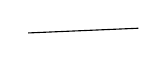
\begin{tikzpicture}
\draw (0,0) -- (1.4,0.06);
\end{tikzpicture}}

Variante de l'étude précédente pour l'extension $G_{\rho,\sigma}$ de
$\mathbb O_{12}^{*}\times H_{S_0}^{+}$ par
$\underline{M}$ (\uline{sans division par}
$\underline{\mu}_G=\{1,\omega\}_{S_0}$). Considérons d'abord la question des
scindages de la sous-extension $\underline{\mathfrak{S}}^{+}$ de
$H_{S_0}^{+}$ par $\underline{M}$ --- \unsure{elles|ils}
correspondent aux couples

\margin{113}
% ===== LM_C4-115-133: second pass, checked against the scans =====
\scanpage{115}
\mspage{705}

\[
\tag{267}
\left\{
\begin{gathered}
\unsure{\rho'}=\zeta\rho,\ \sigma'=\eta\sigma
\quad(\zeta,\eta\in\Gamma\underline M)\quad\text{tels qu'on ait}
\\
\rho'{}^3=\sigma'{}^2=\omega,\qquad
\sigma'(\rho')=\rho'{}^{-1}.
\end{gathered}\right.
\]

(On \unsure{note|notera} qu'un scindage doit transformer $\omega$,
qui opère trivialement sur $\underline M$ et est central
dans $\underline H^+$, dans une \deleted{\unsure{élément}}
\inserted{section} centrale, \unsure{or}
\deleted{\unsure{l'inverse}} \unsure{voir|voici} \unsure{pq} qu'on a
\[
\tag{268}
\left\{\begin{aligned}
\underline M\cap\underline{\mathrm{Cent}}\bigl(\underline{\mathfrak S}^+\bigr)
&=\underline M^{\mathfrak S_3}
=\deleted{\unsure{\{0\}}}\,\unsure{\{1\}|\{0\}},\quad\text{d'où}
\\
\underline{\mathrm{Cent}}\bigl(\underline{\mathfrak S}^+\bigr)
&\simeq\underline\mu_{\underline{\mathfrak S}}
=\{1,\omega\}_{\underline{\mathfrak S}}
\end{aligned}\right.
\]
--- ce qui montre qu'un scindage doit transformer $\omega$ en $\omega$,
d'où \unsure{facilement} la caractérisation (267) des $\rho',\sigma'$
\unsure{correspondants|correspondant} à un scindage).
On en aura
\[
\left\{\begin{aligned}
\rho'{}^3&=(\zeta\rho)^3
=\zeta\rho(\zeta)\rho^2(\zeta)\underbrace{\rho^3}_{\omega}
=\zeta\rho(\zeta)\rho^2(\zeta)\omega
\\
\sigma'{}^2&=(\eta\sigma)^2
=\eta\sigma(\eta)\underbrace{\sigma^2}_{\omega}
=\eta\sigma(\eta)\omega
\end{aligned}\right.
\]
donc les \deleted{deux} équations $\rho'{}^3=\omega$ et
$\sigma'{}^2=\omega$ équivalent respectivement à
\[
\left\{\begin{aligned}
\zeta\rho(\zeta)\rho^2(\zeta)&=1
&\text{i.e.}\quad(1+\rho_M+\rho_M^2)(\zeta)&=0
\\
\eta\sigma(\eta)&=1
&\text{i.e.}\quad(1+\sigma_M)(\eta)&=0
\end{aligned}\right.
\]
i.e. cela se réduit aux équations (245) (246),
et on a vu que la \deleted{solution générale est}
\inserted{\deleted{première} condition}
sur $\zeta$ est automatiquement satisfaite, celle
sur $\eta$ revient à :
\[
(247)\qquad
\eta=b\delta=b(\lambda_1-\lambda_0),\quad
\unsure{\lambda|b}\in\Gamma\mathbb G_a.
\]
La condition $\sigma'(\rho')=\rho'{}^{-1}$ s'explicite d'autre
part comme à la p.~$700'$, on retombe

\margin{114}

\begin{center}
\small
114\\
\texttt{https://grothendieck.umontpellier.fr}\\
Université de Montpellier, UMR CNRS 5149, Case courrier 051, Place Eugène Bataillon\\
34095 Montpellier cedex 5 - France
\end{center}
\scanpage{116}

sur l'équation (249), qui s'explicite par (250).
Cela montre qu'il existe un scindage
$\overline{\mathrm m}$ sur $S_0=\mathrm{Spec}\,\mathbb Z$
--- ce qui revient à un scindage \unsure{du} groupe discret
$\mathfrak S^+$ ext. de
$H^+=\mathfrak S^+/M$
\inserted{$\simeq\mathfrak S_0/\Pi_0$}
(par $M\simeq(\Pi_0)_{\mathrm{ab}}$ \unsure{)}
--- et que les scindages en question forment un
torseur sous $\underline K$, où $K$\inserted{$\simeq\mathbb Z^2$}
est défini dans (253), et en fait \deleted{\unsure{$K$}}
on a un isom $M\simeq K$ (254), soit
$\underline M\simeq\underline K$, \unsure{correspondant}
à l'opération de $\underline M$ sur le \unsure{schéma}
des scindages, par conjugaison. Ainsi on trouve

\uline{Proposition} (Sur une base $S$ quelconque).

L'extension $\underline{\mathfrak S}^+$ de
$\underline H^+$ par $\underline M$ est scindée ---
deux scindages sont conjugués par une unique section
de $\underline M$ --- donc l'application \deleted{de}
``passage au quotient par $\mu_{\mathfrak S}$'' définit une
bijection de l'\unsure{ens.} des scindages de
$\underline{\mathfrak S}^+$ sur $\underline H^+$,
sur l'\unsure{ens.} des scindages de
$\underline{\mathfrak S}^+/\mu_{\underline{\mathfrak S}}$
sur $\underline H^+/\underline\mu_{\underline H^+}
\simeq\underline{\mathfrak S}_3$.

\margin{115}

\begin{center}
\small
115\\
\texttt{https://grothendieck.umontpellier.fr}\\
Université de Montpellier, UMR CNRS 5149, Case courrier 051, Place Eugène Bataillon\\
34095 Montpellier cedex 5 - France
\end{center}
\scanpage{117}
\mspage{706}

Étudions maintenant le centralisateur dans
$\underline G_{\rho,\sigma}$ d'un sous-groupe section
au dessus de $\underline H^+$, \unsure{disons} noté
$\underline H(\rho',\sigma')$. On doit avoir maintenant
\[
\tag{269}
\underline{\mathrm{Cent}}_{\underline G_{\rho,\sigma}}
\bigl(\underline H(\rho',\sigma')\bigr)
\subset
\begin{gathered}
\mathbb O_{12}^*\cdot\bigl(\underline M\times
\underbrace{\mu_{\underline{\mathfrak S}}}_{=\{1,\omega\}_{S_0}}\bigr)
\\[-2pt]
\Vert
\\[-2pt]
\left\{\lambda\omega^i u_{\underline\mu}\ \middle|\
\begin{gathered}
\lambda\in\Gamma\underline M\\
\underline\mu\in\Gamma\mathbb O_{12}^*\\
i\in\Gamma(\unsure{\mathbb Z/2\mathbb Z})_{S_0}
\end{gathered}\right\}
\end{gathered}
\]
D'ailleurs $\lambda\omega^i u_{\underline\mu}$ centralise
$\underline H(\rho',\sigma')$ sss $\lambda u_{\underline\mu}$
centralise. La commutation à $\rho'$ s'explicite encore
par la condition (260), le calcul p.~703 s'appliquant
\unsure{ne varietur}. Pour la condition de commutation à
$\sigma'$, le calcul de p.~$703'$ doit se modifier
car on ne peut plus écrire $\omega^{\nu_2}=1$,
la condition s'écrit
\[
\omega^{\nu_2}\cdot\lambda\eta^{\unsure{\mu}}
\sigma(\lambda^{-1})\sigma=\eta\sigma
\quad\text{i.e.}\quad
\omega^{\nu_2}\lambda\eta^\mu\sigma(\lambda^{-1})=\eta
\]
et équivaut à la conjonction de la condition
\[
\tag{270}
\nu_2(\underline\mu)=0\quad\text{i.e.}\quad
\underline\mu\in\Gamma\mathbb O_{12}^{*\prime\prime},
\]
et de la relation (261). En présence de
$\nu_2(\underline\mu)=0$, les calculs des p.~$703'$, 704
s'appliquent, \unsure{finalement} on trouve :

\uline{Corollaire} Pour tout scindage de
$\underline{\mathfrak S}^+$ au dessus de
$\underline H^+$, \deleted{le commutant}
\inserted{\deleted{\illegible{1}} soit $\underline T$ le centralisateur
\deleted{\unsure{$T$}}} dans $\underline G_{\rho,\sigma}$
du sous-groupe section $\underline H(\rho',\sigma')$,
\deleted{on}

\margin{116}

\begin{center}
\small
116\\
\texttt{https://grothendieck.umontpellier.fr}\\
Université de Montpellier, UMR CNRS 5149, Case courrier 051, Place Eugène Bataillon\\
34095 Montpellier cedex 5 - France
\end{center}
\scanpage{118}

\deleted{\unsure{une section}}\inserted{On a alors} une suite exacte
\[
\tag{271}
\diagram{\begin{tikzcd}[column sep=large]
1 \arrow[r] & \underline\mu_{\unsure{\mathfrak S|G}}
\arrow[r,hook,"{\deleted{\unsure{G}}}" description]
& \underline T \arrow[r] & \mathbb O_{12}^{*\prime\prime}
\arrow[r,no head] & 1
\end{tikzcd}}
\]
et pour $\underline T^{\unsure{\natural|\sharp}}
=\underline T\cap\underline G_{\rho,\sigma}^{\unsure{\natural|\sharp}}$,
on a
\[
\tag{272}
\underline T^{\unsure{\natural|\sharp}}
\simeq\mathbb O_{12}^{*\prime\prime},
\]
i.e. $\underline T^{\unsure{\natural|\sharp}}$ est une section
partielle de $\underline G_{\rho,\sigma}^{\unsure{\natural|\sharp}}$
au dessus de $\mathbb O_{12}^{*\prime\prime}$.

\uline{Corollaire} L'extension $\underline G_{\rho,\sigma}$ de
$\mathbb O_{12}^*\times\underline H^+$ par $\underline M$
n'est scindée sur aucune base $S$ non vide.
L'extension $\underline G_{\rho,\sigma}''$ de
$\mathbb O_{12}^{*\prime\prime}\times\underline H^+$ par
$\underline M$ est scindée sur tte base $S$,
et deux scindages sont conjugués par une unique section de
$\underline M$. L'application naturelle fournit une bijection
de l'\unsure{ens.} des scindages de $\underline G_{\rho,\sigma}''$
sur $\mathbb O_{12}^{*\prime\prime}\times\underline H^+$, avec
l'\unsure{ens.} des scindages de
$\underline{\mathfrak S}^+$ sur $\underline H^+$.

\uline{Corollaire} L'ext. $G_{\rho,\sigma}$ de
$\widehat{\mathbb Z}^{*}\times H^+$ par $M^\wedge$
n'est pas scindée. Celle de $G_{\rho,\sigma}''$ de
$\widehat{\mathbb Z}^{*\prime\prime}\times H^+$ par
$M^\wedge$ est scindée, et deux scindages sont
conjugués par un unique élément \unsure{de} $\widehat M$.
L'application naturelle définit une bijection de l'\unsure{ens.}
des scindages de $G_{\rho,\sigma}''$ sur
$\widehat{\mathbb Z}^{*}\times H^+$ avec l'\unsure{ens.}
des scindages de \deleted{\unsure{$G_\rho$}}
$\mathfrak S^\wedge$ sur $H^+$.

\margin{117}

\begin{center}
\small
117\\
\texttt{https://grothendieck.umontpellier.fr}\\
Université de Montpellier, UMR CNRS 5149, Case courrier 051, Place Eugène Bataillon\\
34095 Montpellier cedex 5 - France
\end{center}
\scanpage{119}
\mspage{707}

Explicitons un scindage de l'extension
$\mathfrak S^+$ de $H^+$ par $M$
--- correspondant à un scindage de
$\underline{\mathfrak S}^+$ de $\underline H^+$
par $\underline M$ --- , via une solution particulière de l'équation
\[
\tag{273}
a_0-2a_1+3b-1=0
\]
en prenant
\[
a_1=b=0\qquad\text{d'où}\qquad a_0=1
\]
i.e.
\[
\tag{274}
\left\{\begin{aligned}
\zeta&=\lambda_0,\ \eta=0\quad\text{(écriture additive)}\\
\rho'&=\lambda_0\rho,\quad\unsure{\sigma'}=\unsure{\sigma}
\end{aligned}\right.
\]
\deleted{le scindage correspondant}
\inserted{les \unsure{trois} formules fournissent un scindage de
$\mathfrak S^+/\mu_{\mathfrak S}$}
au dessus de $\mathfrak S_3
\simeq H^+/\mu_{H^+}$.
Explicitons les \deleted{scindages}\inserted{relèvements}
\unsure{correspondants} de $\mathbb O_{12}^*$ dans
$\underline G_{\rho,\sigma}/\mu_G$ resp. de
$\mathbb O_{12}^{*\prime\prime}$ dans $\underline G_{\rho,\sigma}$\unsure{;},
\[
\tag{275}
\left\{\begin{aligned}
u_{\rho',\sigma'}:\mathbb O_{12}^*&\longrightarrow
\underline G_{\rho,\sigma}/\mu_G
\quad\text{resp.}\quad\mathbb O_{12}^{*\prime\prime}
\mathrel{\text{---}}\underline G_{\rho,\sigma}
\\
\underline\mu&\longmapsto\lambda_\infty^{\nu}u_{\underline\mu}
\qquad(\nu=\nu(\underline\mu))
\end{aligned}\right.
\]
où $u_{\underline\mu}$ défini dans (151).
(NB\unsure{\S} (275) est contenu dans prop. p.~704
(265) et (264), qui donnent
\[
u_{\rho',\sigma'}=\lambda u_{\underline\mu}\qquad
\lambda=x\lambda_0+y\lambda_1\qquad x=y=-\nu
\]
\[
\text{d'où}\qquad\lambda=-\nu(\lambda_0+\lambda_1)=\nu\lambda_\infty.
\]

On aura donc, posant
\[
u'_{\underline\mu}=u_{\rho',\sigma'}(\underline\mu)
\]
\[
\tag{276}
\left\{\begin{aligned}
u'_{\underline\mu}(\rho')&=\rho',\quad
u'_{\underline\mu}(\sigma')=\sigma'\\
u'_{\underline\mu}(\lambda)&=\mu\lambda\quad
(\lambda\in\Gamma\underline M)
\quad\inserted{\text{où}}\ (\mu=\unsure{\chi}(\underline\mu))
\end{aligned}\right\}
\quad\begin{gathered}
\text{(ce qui suffit}\\
\text{à \unsure{conditionner|caractériser}}\ u'_{\underline\mu})
\end{gathered}
\]

\margin{118}

\begin{center}
\small
118\\
\texttt{https://grothendieck.umontpellier.fr}\\
Université de Montpellier, UMR CNRS 5149, Case courrier 051, Place Eugène Bataillon\\
34095 Montpellier cedex 5 - France
\end{center}
\scanpage{120}

et on en déduit aussi
\[
\tag{277}
\left\{
\begin{aligned}
u'_{\underline{\mu}}(\rho)&=\lambda_0^{-2\nu}\rho\\
u'_{\unsure{\mu|\underline{\mu}}}(\sigma)&=\omega^{\nu_2}\sigma
\qquad (=\sigma\text{ dans }\underline G_{\rho,\sigma}/\underline{\mu}_G\ \ldots).
\end{aligned}
\right.
\]

\margin{119}

\begin{center}
\small
119\\
\texttt{https://grothendieck.umontpellier.fr}\\
Université de Montpellier, UMR CNRS 5149, Case courrier 051, Place Eugène Bataillon\\
34095 Montpellier cedex 5 - France
\end{center}
\scanpage{121}
\mspage{708}

13\textsuperscript{o}) \uline{Retour sur la tour de Fermat}.

Commençons par dégager une notion topossique générale, qui \unsure{était} un peu
embrouillée entre les lignes dans 11\textsuperscript{o}).
Soit $\Gamma$ (ici $\Gamma_{\mathbb Q}\times
\mathfrak S_3\deleted{\unsure{)|\}}}=N_{0,3}$) opérant sur
un topos $\mathcal X$ (ici
$\deleted{\unsure{U}}\inserted{\unsure{\mathcal U}_{0,3\overline{\mathbb Q}}}
\simeq M'_{0,4\overline{\mathbb Q}}$) conn.
\inserted{loc. connexe}, \deleted{\unsure{et conn.}} muni d'un ``pt'' (géométrique)
$x_0$ (ici: le point $-\overline j$ à valeurs dans $\overline{\mathbb Q}$), soient
\margin{Contexte discret ($\mathcal X$ loc. simpl. connexe) ou profini,
\unsure{rel.}\illegible{1} \unsure{raisonnables}\ldots}
\[
\tag{278}
\left\{
\begin{aligned}
\Pi&=\Pi_1(\mathcal X,x_0),\qquad
\mathcal M=\Pi_1(\mathcal X,\Gamma;x_0)\\
M&=\Pi_{\mathrm{ab}}=\Pi/[\Pi,\Pi],\qquad
\deleted{\unsure{\mathfrak S}}\inserted{\widetilde{\mathcal M}}
=\mathcal M/[\Pi,\Pi],\qquad \deleted{\text{d'où}}
\end{aligned}
\right.
\]
d'où des suites exactes et hom. de suites exactes
\[
\tag{279}
\diagram{\begin{tikzcd}[column sep=large,row sep=large]
1 \arrow[r,dash] & \Pi \arrow[r] \arrow[d,"\text{épi}"]
& \mathcal M \arrow[r] \arrow[d,"\text{épi}"]
& \Gamma \arrow[r,dash] \arrow[d,"\unsure{\sim|\wr}"] & 1\\
1 \arrow[r,dash] & M \arrow[r,dash]
& \deleted{\unsure{\mathfrak S}}\inserted{\widetilde{\mathcal M}} \arrow[r]
& \Gamma \arrow[r,dash] & 1
\end{tikzcd}}\ .
\]

\deleted{Considérons}
\inserted{(Au lieu de prendre
$M=\Pi/\unsure{(\Pi,\Pi)|[\Pi,\Pi]}\inserted{=\Pi_{\mathrm{ab}}}$,}
on \unsure{aurait|avait} pu prendre un quotient de $\Pi_{\mathrm{ab}}$ invariant par
action de $\Gamma$, mais peu importe\ldots).
Considérons ``le rev. universel abélien'' \inserted{$\mathcal X'_0$} de
$\mathcal X$ en $x_0$, i.e. le quotient par $[\Pi,\Pi]$ du rev. universel de
$\mathcal X$ en $x_0$ --- c'est donc un rev. principal de $\mathcal X$, de
groupe $M$. On

\margin{120}

\begin{center}
\small
120\\
\texttt{https://grothendieck.umontpellier.fr}\\
Université de Montpellier, UMR CNRS 5149, Case courrier 051, Place Eugène Bataillon\\
34095 Montpellier cedex 5 - France
\end{center}
\scanpage{122}

se propose d'examiner les façons de \deleted{prolonger}\inserted{relever}
l'action de $\Gamma$ sur $\mathcal X$ \deleted{(via $M$)} en une
action \deleted{de $\mathcal M$}\inserted{sur $\mathcal X'_0$}, compatible
avec l'action \inserted{de $\Gamma$ sur le groupe d'opérateurs $M$}
\deleted{sur $\mathcal X$ via $\Gamma$,
\inserted{et prolonger l'action de
$M\subset\mathfrak S$,}
\unsure{ou ce qui} \unsure{revient} au $\overline{\mathrm m}$, par une action de
$\mathfrak S$, compatible avec son action sur
$\mathcal X$ (via $\Gamma$)}.
Plus généralement, si $\mathcal X'$ est un $M_{\mathcal X}$-torseur sur
$\mathcal X$ isomorphe \unsure{à} $\mathcal X'_0$, donc déduit
\deleted{\unsure{par un}}\inserted{de $\mathcal X'_0$} par twist à l'aide
d'un $M$-torseur $E$ ($\unsure{\simeq|=}$ fibre de $\mathcal X'_0$ en $x_0$),
étudions les \deleted{extensions}\inserted{relèvements} analogues de l'action
de $\deleted{\unsure{\mathfrak S}}\inserted{\Gamma}$ sur $\mathcal X$ en une
action de $\deleted{\unsure{\mathfrak S}}\inserted{\Gamma\text{ sur }\mathcal X'}$,
compatible avec l'action de
$\deleted{\unsure{\mathfrak S}}\inserted{\Gamma}$ sur $\mathcal X$.

\deleted{Notons que, si $\widetilde{\mathcal X}$ désigne le rev. universel de
$\mathcal X$ en $x_0$, $\mathcal M$ opère sur $\widetilde{\mathcal X}$ de façon
compatible avec son action sur $\mathcal X$, \unsure{en|et} prolongeant l'action
\inserted{canonique} de $\Pi$ sur $\widetilde{\mathcal X}$ --- comme
$[\Pi,\Pi]\subset\Pi$ est distingué dans $\mathcal M$, cette action passe au
quotient en une action canonique de
$\mathfrak S=\mathcal M/[\Pi,\Pi]$ sur
$\mathcal X'_0=\widetilde{\mathcal X}/[\Pi,\Pi]$, qui satisfait aux}

\margin{121}

\begin{center}
\small
121\\
\texttt{https://grothendieck.umontpellier.fr}\\
Université de Montpellier, UMR CNRS 5149, Case courrier 051, Place Eugène Bataillon\\
34095 Montpellier cedex 5 - France
\end{center}
\scanpage{123}
\mspage{709}

\deleted{\inserted{deux} conditions envisagées. Soit $\Theta_0$ cette
opération-ci de $\mathfrak S$, et $\Theta$ une opération
quelconque, satisfaisant aux dites conditions.}

On veut donc faire de $\mathcal X'$, qui est un rev. de $\mathcal X$, donné
par sa fibre $E$ en $x_0$ et l'action de $\Pi=\Pi_1(\mathcal X,x_0)$ sur
$E$ (par translations, grâce à une structure de $M$ torseur sur $E$) un
revêtement de $(\mathcal X',\deleted{\unsure{\mathfrak S}}\inserted{\Gamma})$
--- i.e. \uline{prolonger} l'action donnée de $\Pi$ sur \unsure{la|le} fibre
$E$, en une action de $\mathcal M$ sur $E$ --- qui d'ailleurs se factorise
nécessairement par
$\deleted{\unsure{\mathfrak S}}\inserted{\widetilde{\mathcal M}}$.
Je dis que cette action se fait néc\textsuperscript{t} \unsure{à} travers le
groupe affine du torseur $E$ --- de façon précise, $\Gamma$ opère sur $M$,
\unsure{soit} $\gamma_M$ l'opération définie par $\gamma\in\Gamma$, et soit
$g\in\deleted{\unsure{\mathfrak S}}\inserted{\widetilde{\mathcal M}}$ au dessus de
$\gamma\in\Gamma$, on aura donc, pour $x\in E$, $\lambda\in M$
\[
\tag{280}
\diagram{\begin{tikzcd}[column sep=0em,row sep=0.6em]
g & (\lambda & {}\cdot{} & x & {})=\gamma_M(\lambda)\mathbin{.}gx\\
\deleted{\unsure{\mathfrak S}}\inserted{\widetilde{\mathcal M}}
\arrow[u,phantom,"\in"{description,rotate=-90}]
& M\arrow[u,phantom,"\in"{description,rotate=-90}]
& & E\arrow[u,phantom,"\in"{description,rotate=-90}] &
\end{tikzcd}}
\]
ce qui \unsure{est} trivial par le calcul.
\deleted{\unsure{car|est}}
\[
g(\lambda.x)=(g\lambda)x=(g\lambda g^{-1}g)x
=\underbrace{(g\lambda g^{-1})}_{\gamma_M(\lambda)}.(gx)
\]

\margin{122}

\begin{center}
\small
122\\
\texttt{https://grothendieck.umontpellier.fr}\\
Université de Montpellier, UMR CNRS 5149, Case courrier 051, Place Eugène Bataillon\\
34095 Montpellier cedex 5 - France
\end{center}
\scanpage{124}

Donc si on introduit le groupe $\operatorname{Aff}(E)$, on aura un
homomorphisme de suites exactes
\[
\tag{281}
\diagram{\begin{tikzcd}[column sep=large,row sep=large]
1 \arrow[r] & M \arrow[r,dash]
\arrow[d,Rightarrow,"{\deleted{\unsure{\Theta}}\mathrm{id}_M}"]
& \deleted{\unsure{\mathfrak S}}
\inserted{\widetilde{\mathcal M}} \arrow[r]
\arrow[d,"{\Theta_{\deleted{\unsure{\mathfrak S}}\inserted{\widetilde{\mathcal M}}}}"]
& \Gamma \arrow[r,dash] \arrow[d,"\Theta_\Gamma"] & 1\\
1 \arrow[r,dash] & M \arrow[r]
& \operatorname{Aff}(E) \arrow[r]
& \operatorname{Aut}(M) \arrow[r] & 1
\end{tikzcd}}
\]
où les flèches verticales extrêmes $\mathrm{id}_M$ \inserted{et
$\Theta_\Gamma$} sont connues, et où la flèche médiane est à déterminer.
On peut dire que la catégorie des $\mathcal X'$ \unsure{cherchés|cherchées}
(avec l'op. de $\Gamma$ dessus satisfaisant aux conditions voulues)
\inserted{est} équivalente à celle des couples
$(E,\Theta_{\deleted{\unsure{\mathfrak S}}\inserted{\widetilde{\mathcal M}}})$,
où $E$ est un $M$-torseur, et
$\Theta_{\deleted{\unsure{\mathfrak S}}\inserted{\widetilde{\mathcal M}}}$
un hom de groupes
$\deleted{\unsure{\mathfrak S}}\inserted{\widetilde{\mathcal M}}
\longrightarrow\operatorname{Aff}(E)$ \deleted{\unsure{rendant}}
compatible avec $\mathrm{id}_M$ et $\Theta_\Gamma$ i.e. qui
\unsure{rende|rend} commutatif (281).
On peut dire aussi: une fois $E$ choisi,
\inserted{(et ce choix est \unsure{anodin} à isom non unique
près\unsure{!!!|\ldots})}
que cela définit une extension $\operatorname{Aff}(E)$ de
$\operatorname{Aut}(M)$ par $M$, d'où grâce à
$\Gamma\longrightarrow\operatorname{Aut}(M)$ une
extension

\margin{123}

\begin{center}
\small
123\\
\texttt{https://grothendieck.umontpellier.fr}\\
Université de Montpellier, UMR CNRS 5149, Case courrier 051, Place Eugène Bataillon\\
34095 Montpellier cedex 5 - France
\end{center}
\scanpage{125}
\mspage{\textcircled{710}}

\margin{les scindages de $\operatorname{Aff}(E)$ déterminés par les pts de $E$ -- \unsure{dépt} de l'origine \unsure{scindages} \unsure{intérieurs}\ldots}

par $M$, \inserted{qui est \uline{d'ailleurs scindée}.} (Ceci dit, les relèvements d'action de $\Gamma$ dessus correspondent aux isomorphismes de cette extension de $\Gamma$ par $M$, avec l'extension $\mathfrak S$ elle-$\overline{\mathrm m}$. Donc elle existe sss l'extension de $\mathfrak S$ de $\Gamma$ par $M$ est scindée, \deleted{\unsure{ce qui}} \inserted{i.e.\ \unsure{l'expression}}
\[
c^2(\mathfrak S)\in H^2(\Gamma,M)\quad\text{est nulle.}
\tag{282}
\]
S'il existe un tel relèvement i.e. un tel isomorphisme, ceux-ci forment un torseur \unsure{sous|sur} le groupe des autom. de l'extension (triviale) $\mathfrak S$ de $\Gamma$ par $M$ qui s'identifie au groupe
\[
(\qquad Z^1(\Gamma,M)
\]
des homomorphismes croisés de $\Gamma$ dans $M$. Les classes de $M$-conjugaison de tels \deleted{relèvements \unsure{(ou}} isomorphismes correspondent donc aux éléments de
\[
H^1(\Gamma,M).
\]

Une autre façon de le dire, en prenant $E={}$\inserted{$M$-}torseur trivial${}=M$, donc $\operatorname{Aff}(E)$ scindé, c'est que les relèvements choisis correspondent aux \uline{scindages} de l'extension $\mathfrak S$ de $\Gamma$ par $M$, et les classes de \inserted{$M$-}conjugaison des relèvements d'action de $\Gamma$ sur $\mathcal X'_0$

\margin{124}

\begin{center}
\small
124\\
\texttt{https://grothendieck.umontpellier.fr}\\
Université de Montpellier, UMR CNRS 5149, Case courrier 051, Place Eugène Bataillon\\
34095 Montpellier cedex 5 - France
\end{center}
\scanpage{126}

correspondent aux classes de $M$-conjugaison des scindages de ladite extension $\mathfrak S$ de $\Gamma$ par $M$.

Ceci bien posé, revenons à la situation de
\[
\left(\underbrace{U_{0,3\overline{\mathbb Q}}}_{\mathcal X},\quad
\Gamma=\underbrace{\Gamma_{\mathbb Q}\times\mathfrak S_3}_{N_{0,3}}\right),
\]
les $\Gamma$-revêtements de $\mathcal X$ correspondent aux $\mathfrak S_3$-revêtements de $U_{0,3\mathbb Q}$, i.e. aux rev. de $(U_{0,3\mathbb Q},\mathfrak S_3)$.

\margin{\uline{NB} Le groupe qu'on vient de noter $M$ devient ici $\unsure{\widehat M}$, $\mathcal M$ devient $\mathcal M_{0,3}$, $\pi$ devient $\widehat\Pi_{0,3}$.}

À l'aide des constructions générales du \S~49 $\overline{\uline{\mathrm{VI}}}$, \deleted{on a déduit} du quotient
\[
\deleted{\unsure{G_{\rho,\sigma}}=\unsure{\mathfrak S}^{+\wedge}/\unsure{\mu_G}\simeq
\operatorname{SL}(2,\mathbb Z)^\wedge/
[\unsure{\widehat\Pi_{0,3}},\unsure{\widehat\Pi_{0,3}}]}
\]
\[
\mathfrak S^{+\wedge}/\mu_{\mathfrak S}\simeq
\unsure{\mathcal M}_{0,3}^{+}/[\widehat\Pi_{0,3},\widehat\Pi_{0,3}]
\subset\widetilde{\mathcal M}
\]
\deleted{est}

\margin{on pourrait le noter $\unsure{\widetilde{\mathcal M}'}$!}

\deleted{ext} (avec les notations des pages précédentes), extension de $\mathfrak S_3\subset\Gamma(=\Gamma_{\mathbb Q}\times\mathfrak S_3)$ par $M^\wedge$, on a \inserted{déduit} un groupe profini, \deleted{\unsure{et}} qui était noté $G_{\rho,\sigma}/\mu_G$ \inserted{ou $G_{\rho,\widetilde\sigma}$} dans les sections précédentes et y apparaissait comme un produit $\frac12$-direct
\[
G_{\rho,\widetilde\sigma}
=\deleted{\unsure{\mathbb O|\Phi}}\widehat{\mathbb Z}^{*}\mathbin{.}\widetilde{\mathcal M},
\qquad\text{ext. de }\widehat{\mathbb Z}^{*}\times\mathfrak S_3
\quad\text{par }M^\wedge
\]
et un hom. canonique
\[
\widetilde{\mathcal M}
=\mathcal M_{0,3}/(\widehat\Pi_{0,3},\widehat\Pi_{0,3})
\longrightarrow G_{\rho,\widetilde\sigma}
\]
s'insérant dans un hom. de suites exactes

\margin{125}

\begin{center}
\small
125\\
\texttt{https://grothendieck.umontpellier.fr}\\
Université de Montpellier, UMR CNRS 5149, Case courrier 051, Place Eugène Bataillon\\
34095 Montpellier cedex 5 - France
\end{center}
\scanpage{127}
\mspage{711}

\diagram{
\[
\begin{tikzcd}[column sep=large,row sep=huge]
1 \arrow[r,no head] &
\widehat M \arrow[r] \arrow[d,Rightarrow] &
\widetilde{\mathcal M} \arrow[r] \arrow[d] &
\underbrace{\Gamma}_{N_{0,3}=\Gamma_{\mathbb Q}\times\mathfrak S_3}
\arrow[r,no head] \arrow[d,"\unsure{\chi}\times\operatorname{id}_{\mathfrak S_3}"] & 1 \\
1 \arrow[r,no head] &
\widehat M \arrow[r,no head] &
G_{\rho,\widetilde\sigma} \arrow[r] &
\widehat{\mathbb Z}^{*}\times\mathfrak S_3 \arrow[r,no head] & 1 .
\end{tikzcd}
\tag{282}
\]
}

D'ailleurs contre \unsure{tte|toute} attente on a trouvé que l'extension $G_{\rho,\widetilde\sigma}$ de $\widehat{\mathbb Z}^{*}\times\mathfrak S_3$ par $\widehat M$ était scindée, d'où il résulte que \deleted{celle de} l'ext. $\widetilde{\mathcal M}$. de $\Gamma$ par $\widehat M$ l'est aussi (\deleted{ce qui \unsure{précède|précédait}} \inserted{ce dernier fait} est aussi conséquence de l'existence de la tour de Fermat, en y appliquant les réflexions générales des pages précédentes). Bien mieux, on a vu qu'il y a une unique classe de $\widehat M$-conj. de scindages de l'extension $G_{\rho,\widetilde\sigma}$, ce qui induit une classe de $\widehat M$-conjugaison \uline{canonique} (mais non unique!) de \deleted{$\unsure{\widehat M}$} scindages de $\widetilde{\mathcal M}$ au-dessus de $\Gamma$. Cela définit donc une classe d'\deleted{isomorphie}\inserted{$\widehat M$-conjugaison} canonique de relèvements de l'action de $\Gamma$ \inserted{sur $\mathcal X=U_{0,3\overline{\mathbb Q}}$} à $\mathcal X'_0$ -- ou ce qui revient au $\overline{\mathrm m}$, un torseur sur $(U_{0,3\mathbb Q},\mathfrak S_3)$, de groupe un groupe profini

\margin{\uline{NB} $H^1(\Gamma,\widehat M)$ est un groupe fort gros! -- Mais voir \unsure{ci-dessous}, cf Th. p.~716}

\margin{126}

\begin{center}
\small
126\\
\texttt{https://grothendieck.umontpellier.fr}\\
Université de Montpellier, UMR CNRS 5149, Case courrier 051, Place Eugène Bataillon\\
34095 Montpellier cedex 5 - France
\end{center}
\scanpage{128}

commutatif au dessus de $(U_{0,3\mathbb Q},\mathfrak S_3)$ qui au dessus de \deleted{$U_{0,3\unsure{\overline{\mathbb Q}}}$ \illegible{2}} \inserted{$U_{0,3\overline{\mathbb Q}}$ soit isomorphe} au rev. $\mathcal X'_0$ envisagé plus haut.

Revenons pour un instant à ce cas général du début. Notons que la donnée d'un diagramme (281) \deleted{imposant} définit un quotient \inserted{$\widetilde{\widetilde{\mathcal M}}$} de $\widetilde{\mathcal M}$ -- à savoir le coimage de $\Theta_{\widetilde{\mathcal M}}$ -- \deleted{\unsure{donnant} lieu à une suite} \inserted{tel que $M\hookrightarrow\widetilde{\widetilde{\mathcal M}}$ soit injectif, et} donnant donc lieu à une suite \deleted{exacte} exacte
\diagram{
\[
\begin{tikzcd}[column sep=large,row sep=large]
1 \arrow[r,no head] & M \arrow[r,no head] &
\widetilde{\widetilde{\mathcal M}} \arrow[r,no head] &
\widetilde\Gamma \arrow[r,no head] \arrow[d,equal,"\mathrm{déf}"] & 1, \\
& & & \widetilde{\widetilde{\mathcal M}}/\operatorname{Im}M &
\end{tikzcd}
\tag{283}
\]
}
\unsure{puis|où} on a
\diagram{
\[
\begin{tikzcd}[column sep=large]
\widetilde\Gamma \arrow[r,hook] & \operatorname{Aut}(M),
\end{tikzcd}
\tag{284}
\]
}
$\widetilde\Gamma$ s'identifie à l'image de $\Gamma$ dans $\operatorname{Aut}(M)$ par l'action de $\Gamma$ sur $M$ provenant de la structure d'ext. $\widetilde{\mathcal M}$ de $\Gamma$ par $M$.

\deleted{Cette} Ce quotient $\widetilde{\widetilde{\mathcal M}}$ de $\mathcal M$, donnant naissance à une ext. (283), n'est pas quelconque -- à part le fait que $M$ s'y envoie injectivement, et que $\widetilde\Gamma=\widetilde{\widetilde{\mathcal M}}/\operatorname{Im}M$

\margin{127}

\begin{center}
\small
127\\
\texttt{https://grothendieck.umontpellier.fr}\\
Université de Montpellier, UMR CNRS 5149, Case courrier 051, Place Eugène Bataillon\\
34095 Montpellier cedex 5 - France
\end{center}
\scanpage{129}
\mspage{712}

opère \deleted{\unsure{injective|injectivement}} \inserted{\uline{fidèlement}} sur $M$ : en plus, l'extension (283) est triviale, et \deleted{en fait} \inserted{le fait} qu'elle provienne d'un $\Theta_{\widetilde{\mathcal M}}$ implique une \uline{structure supplémentaire} sur cette extension, à savoir la donnée d'une classe de $M$-conjugaison de scindages.

Plus précisément, on aura une application canonique
\diagram{
\[
\begin{tikzcd}[column sep=large]
E \arrow[r] & \operatorname{Scind}\bigl(\widetilde{\widetilde{\mathcal M}}\ \text{\unsure{comme|conçue} ext de }\widetilde\Gamma\text{ par }M\bigr)
\end{tikzcd}
\tag{285}
\]
}
compatible avec les opérations de $M$ sur $E$ (par translation) et sur $\operatorname{Scind}$ (par composition \unsure{avec|ou} \unsure{autom.|automs} intérieurs).
\inserted{La classe de $M$-conjugaison envisagée de scindages n'est autre que l'image de $E$.}

Pour que $x$ et $y\in E$ aient $\overline{\mathrm m}$ image dans $\operatorname{Scind}$, il f et s. que l'élément $u=y-x\in M$ soit dans $M^\Gamma=M^{\widetilde\Gamma}$, ce qui montre que
\diagram{
\[
\begin{tikzcd}[column sep=large,row sep=large]
\text{l'hom }E \arrow[r,no head] & \operatorname{Scind}\text{ est injectif} \\
& \text{sss}\quad M^\Gamma=\{0\}\quad .
\end{tikzcd}
\tag{286}
\]
}

Dans le cas où $M^\Gamma=\{0\}$, on voit donc que $E$ s'identifie exactement à une classe de $M$-conjugaison des scindages de $\widetilde{\widetilde{\mathcal M}}$.

\margin{128}

\begin{center}
\small
128\\
\texttt{https://grothendieck.umontpellier.fr}\\
Université de Montpellier, UMR CNRS 5149, Case courrier 051, Place Eugène Bataillon\\
34095 Montpellier cedex 5 - France
\end{center}
\scanpage{130}

Résumons ces considérations, dans une

\uline{Proposition} Soient $\mathcal X$ un topos \deleted{\unsure{c}} connexe loc. connexe muni d'un pt géom. $x_0$, on se place dans le contexte discret ($\mathcal X$ \unsure{loc.|loc} \unsure{simpl|simpl.} connexe) ou profini (revêtement signifie revêtement profini).
\margin{\figure{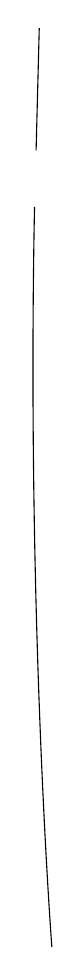
\begin{tikzpicture}[x=1cm,y=1cm]
\draw (0,0) -- (-0.04,-1.55);
\draw (-0.06,-2.27) .. controls (-0.14,-6.3) and (0.04,-10.0) .. (0.16,-11.67);
\end{tikzpicture}}}

On a un groupe $\Gamma$ d'\unsure{autom} de $\mathcal X$ ($\Gamma$ profini dans le cas profini --- il faudrait expliciter pour bien faire les hypothèses raisonnables à faire pour tenir compte de la topologie profinie de $\Gamma$\ldots). On pose
\[
\Pi=\Pi_1(\mathcal X,x_0),\quad \mathcal M=\Pi_1(\mathcal X,\Gamma;x_0)\qquad\text{d'où}
\]
\inserted{\diagram{\begin{tikzcd}[column sep=large]
{(*)}\quad 1 \arrow[r,no head] & \Pi \arrow[r,no head] & \mathcal M \arrow[r,no head] & \Gamma \arrow[r] & 1
\end{tikzcd}}}
on se donne un quotient $M$ de $\Pi$, \deleted{\unsure{un}} par un sous-groupe distingué \uline{dans $\mathcal M$}, \unsure{ou} ce qui revient au $\overline{\mathrm m}$ un quotient de $\Pi_{\mathrm{ab}}=\Pi/[\Pi,\Pi]$ stable par l'action de $\Gamma$, \deleted{pour}\inserted{d'où} une \deleted{$\widetilde{\mathcal M}=\mathcal M/$} extension quotient de $(*)$,
\[
(287)\qquad
\diagram{\begin{tikzcd}[column sep=large]
1 \arrow[r] & M \arrow[r,no head] & \widetilde{\mathcal M} \arrow[r,no head] & \Gamma \arrow[r,no head] & 1
\end{tikzcd}}
\]
où $M$ est \unsure{comm|comm.} donc $\Gamma$ opère sur $M$.

On s'intéresse à la catégorie des revêtements \deleted{$\unsure{M_{\mathcal X}}$-torseurs $\mathcal X'_0$ \unsure{sur}} $\mathcal X'$ de $(\mathcal X,\Gamma)$, satisfaisant les conditions

\margin{129}

\begin{center}
\small
129\\
\texttt{https://grothendieck.umontpellier.fr}\\
Université de Montpellier, UMR CNRS 5149, Case courrier 051, Place Eugène Bataillon\\
34095 Montpellier cedex 5 - France
\end{center}
\scanpage{131}
\mspage{713}

Suivantes : après oubli des opérations de $\Gamma$, on trouve un revêtement \inserted{connexe} galoisien \inserted{\unsure{(et $\overline{\mathrm m}$ abélien)}} de $\mathcal X$, correspondant au groupe quotient $M$ de $\Pi=\Pi_1(\mathcal X,x_0)$ --- de sorte que $\mathcal X'$ devient de façon naturelle un torseur sous $M_{\mathcal X}$.
\margin{\figure{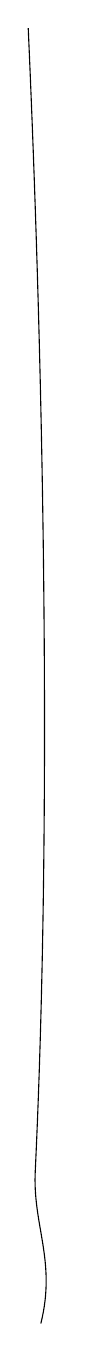
\begin{tikzpicture}[x=1cm,y=1cm]
\draw (0,0) .. controls (0.2,-4.5) and (0.3,-10.0) .. (0.09,-14.5) .. controls (0.05,-15.2) and (0.36,-15.65) .. (0.16,-16.45);
\end{tikzpicture}}}
Le foncteur
\[
\mathcal X'\longmapsto\mathcal X'(x_0)\qquad\text{(fibre en $x_0$)}
\]
de la catégorie de ces $\mathcal X'$ dans la catégorie des ensembles, s'en va en fait vers les ensembles $E$ munis des structures suivantes

\noindent a) $E$ est un $M$-torseur, et en tant que tel donne naissance à une extension
\diagram{\begin{tikzcd}[column sep=large]
1 \arrow[r,no head] & M \arrow[r] & \operatorname{Aff}(E) \arrow[r] & \operatorname{Aut}(M) \arrow[r,no head] & 1
\end{tikzcd}}
d'où une sous-extension \unsure{induite}
\[
(288)\qquad
\diagram{\begin{tikzcd}[column sep=large]
1 \arrow[r,no head] & M \arrow[r,no head] & \operatorname{Aff}_{\Gamma}(E) \arrow[r] & \widetilde\Gamma \arrow[r,no head] & 1
\end{tikzcd}}
\]
où
\[
\widetilde\Gamma=\operatorname{Im}(\Gamma\longrightarrow\operatorname{Aut}(M)).
\]

\noindent b) On a un hom d'extensions
\[
(289)\qquad
\diagram{\begin{tikzcd}[column sep=large,row sep=large]
1 \arrow[r,no head] & M \arrow[r,no head] \arrow[d,Rightarrow,"\mathrm{id}"] & \widetilde{\mathcal M} \arrow[r,no head] \arrow[d,"\Theta_{\widetilde{\mathcal M}}"] & \Gamma \arrow[r,no head] \arrow[d,"\mathrm{can}"] & 1 \\
1 \arrow[r,no head] & M \arrow[r,no head] & \operatorname{Aff}_{\Gamma}(E) \arrow[r,no head] & \widetilde\Gamma \arrow[r,no head] & 1
\end{tikzcd}}\qquad .
\]
La catégorie des $\mathcal X'$ (avec iso\ldots) équivaut à celle des \deleted{$\unsure{M}$} couples $(E,\Theta_{\widetilde{\mathcal M}})$, où $E$ est un $M$-torseur, et $\Theta_{\widetilde{\mathcal M}}$ un hom d'extensions (289).

\margin{130}

\begin{center}
\small
130\\
\texttt{https://grothendieck.umontpellier.fr}\\
Université de Montpellier, UMR CNRS 5149, Case courrier 051, Place Eugène Bataillon\\
34095 Montpellier cedex 5 - France
\end{center}
\scanpage{132}

Les autom. d'un objet $\mathcal X'$ correspondent aux ``translations'' par des éléments de $M^\Gamma$\inserted{$=\operatorname{Cent}(\widetilde{\mathcal M})$}, (\unsure{en} les termes de $E,\Theta_{\widetilde{\mathcal M}}$) aux translations de $E$ par des \deleted{tels \unsure{éléments|élém.}} éléments de $M^\Gamma$, \deleted{qui en \unsure{tant}}\inserted{(en tant} qu'éléments de $\operatorname{Aff}_{\Gamma}(E)$ ils sont centraux, et en conjuguant par ces éléments on trouve le \uline{$\overline{\mathrm m}$} hom $\Theta_{\widetilde{\mathcal M}}$\ldots).
\margin{\figure{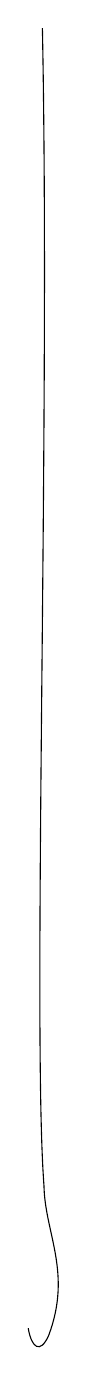
\begin{tikzpicture}[x=1cm,y=1cm]
\draw (0,0) .. controls (0.10,-5.0) and (-0.13,-12.7) .. (0.02,-14.7) .. controls (0.03,-15.3) and (0.38,-15.8) .. (0.08,-16.6) .. controls (-0.03,-16.85) and (-0.14,-16.75) .. (-0.18,-16.51);
\end{tikzpicture}}}
Les classes d'isomorphie de tels \unsure{éléments} \deleted{\unsure{s'identifient}}\inserted{\unsure{correspondent}} biunivoquement aux classes de $M$-conjugaison des scindages de l'extension (287) de $\Gamma$ par $\widetilde{\mathcal M}$. De façon précise, à un $(E,\Theta_{\widetilde{\mathcal M}})$ est associé \unsure{canonique|canoniquement} un \deleted{$\unsure{M}$} homomorphisme de $M$-ensembles
\[
(290)\qquad
\diagram{\begin{tikzcd}[column sep=large]
E \arrow[r] & \operatorname{Scind}(\widetilde{\mathcal M}\ \unsure{\text{ext.}}\ \text{de }\Gamma\ \text{par }M)
\end{tikzcd}}
\]
dont l'image est la classe de conjugaison \unsure{décrivant} la classe d'isomorphie envisagée. \deleted{\unsure{L'image}}\inserted{L'hom} (290) \unsure{se|de} factorise par $M^\Gamma\backslash E$ en un \uline{mono}
\[
(291)\qquad
\diagram{\begin{tikzcd}[column sep=large]
M^\Gamma\backslash E \arrow[r,hook] & \operatorname{Scind}(\widetilde{\mathcal M}\ \text{ext. de }\Gamma\ \text{par }M)
\end{tikzcd}},
\]
et si $M^\Gamma=0$, on voit que $E$ se reconstitue canoniquement à partir de la classe de

\margin{131}

\begin{center}
\small
131\\
\texttt{https://grothendieck.umontpellier.fr}\\
Université de Montpellier, UMR CNRS 5149, Case courrier 051, Place Eugène Bataillon\\
34095 Montpellier cedex 5 - France
\end{center}
\scanpage{133}
\mspage{714}

conjugaison envisagée. L'opération \inserted{(affine)} de $\widetilde{\mathcal M}$ sur $E$ \inserted{(définie par $\Theta_{\widetilde{\mathcal M}}$)} n'est autre que l'opération \deleted{de} \inserted{(\unsure{induite} par la)} conjugaison sur \inserted{l'ens} des scindages (qui bien entendu ne fait pas sortir d'une classe de $M$-conjugaison, $\overline{\mathrm m}$ en conjuguant par des éléments quelconques de $\widetilde{\mathcal M}$).
\margin{\figure{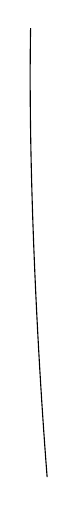
\begin{tikzpicture}[x=1cm,y=1cm]
\draw (0,0) .. controls (-0.03,-1.65) and (0.07,-3.9) .. (0.21,-5.7);
\end{tikzpicture}}}

\uline{Corollaire} Supposons que l'on ait
\[
(292)\qquad \underbrace{H^0(\widetilde\Gamma,M)}_{M^\Gamma}=H^1(\widetilde\Gamma,M)=0
\]
i.e. que \deleted{\unsure{toutes|tous}} deux scindages d'une ext. triviale de $\widetilde\Gamma$ par $M$ soient conjugués par un élément unique de $M$. Cela implique \inserted{donc (à cause de $M^\Gamma=\unsure{\{0\}|0}$)} que la catégorie des $\mathcal X'$, ou encore celle des couples $(E,\Theta_{\widetilde{\mathcal M}})$, est rigide, \deleted{Alors les classes} \inserted{i.e. un objet est connu à isom.} unique près quand on connait sa classe d'isomorphie. Ceci posé, les classes d'isomorphie en question \deleted{correspondent}\inserted{(i.e. les classes} de \deleted{$M$-\unsure{conj|conj.}} conjugaison des scindages de \deleted{biunivoquement} l'ext. $\widetilde{\mathcal M}$ de $\Gamma$ par $M$) correspondent biunivoquement aux groupes quotients $\widetilde{\widetilde{\mathcal M}}$
\margin{\figure{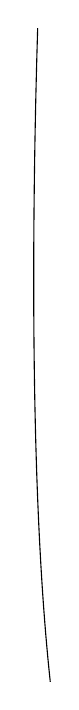
\begin{tikzpicture}[x=1cm,y=1cm]
\draw (0,0) .. controls (-0.06,-1.95) and (-0.12,-5.7) .. (0.16,-8.3);
\end{tikzpicture}}}

\margin{132}

\begin{center}
\small
132\\
\texttt{https://grothendieck.umontpellier.fr}\\
Université de Montpellier, UMR CNRS 5149, Case courrier 051, Place Eugène Bataillon\\
34095 Montpellier cedex 5 - France
\end{center}
% ===== LM_C4-134-152: first pass only (not yet checked) =====
\scanpage{134}

\margin{\figure{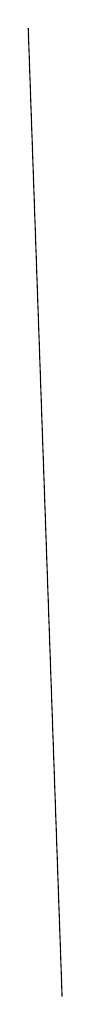
\begin{tikzpicture}\draw (0,0) -- (0.43,-12.3);\end{tikzpicture}}}

de $\mathcal M$ satisfaisant aux conditions suivantes

\par a) $M\longrightarrow\widetilde{\widetilde{\mathcal M}}$ (\unsure{composé} $M\longrightarrow\unsure{\widetilde{\mathcal M}|\overline{\mathcal M}}\longrightarrow\widetilde{\widetilde{\mathcal M}}$) est injectif,

\par \deleted{b) $\unsure{\Gamma'}\ \widetilde{\widetilde{\mathcal M}}/\unsure{M|\Gamma}$}

\par d'où extension

\par $(293)$\quad
\diagram{\begin{tikzcd}[ampersand replacement=\&,column sep=small]
1\arrow[r,dash]\&M\arrow[r,dash]\&\widetilde{\widetilde{\mathcal M}}\arrow[r,dash]\&\deleted{\unsure{\widetilde{\widetilde{\mathcal M}}/M}}\,\underset{\inserted{\overset{\mathrm{dfn}}{=}\widetilde{\widetilde{\mathcal M}}/M}}{\Gamma'}\arrow[r,dash]\&1
\end{tikzcd}}

\par b) \deleted{$\unsure{\widetilde{\widetilde{\mathcal M}}/M}$} $\Gamma'\overset{\mathrm{dfn}}{=}\widetilde{\widetilde{\mathcal M}}/M$ opère \uline{\unsure{fidèlement}} sur $M$,

\par i.e. on a
\[
\Gamma'\simeq\widetilde\Gamma=\operatorname{Im}(\Gamma\longrightarrow\operatorname{Aut}(M)).
\]

\par c) L'extension $\widetilde{\widetilde{\mathcal M}}$ de $\Gamma'\simeq\widetilde\Gamma$ par $M$ est triviale (i.e. sa classe dans $H^2(\widetilde\Gamma,M)$ est nulle).

\par Pour un tel quotient $\widetilde{\widetilde{\mathcal M}}$\inserted{ de $\widetilde{\mathcal M}$}, on récupère $E$ comme l'ensemble de tous les scindages de l'extension $\widetilde{\widetilde{\mathcal M}}$ de $\widetilde\Gamma$ par $M$, \deleted{\unsure{que}} sur lequel on fait opérer $\widetilde{\mathcal M}$ via $\widetilde{\widetilde{\mathcal M}}$ par conjugaison -- la restriction de cette opération à $M\subset\widetilde{\mathcal M}$ fait de $E$ un $\unsure{E}$-torseur (par l'hyp. $(292)$).


Revenons à nouveau au cas particulier qui nous intéresse. Au n\textsuperscript{o} précédent $(12^{\mathrm o})$ nous avons vérifié les trois relations $(292)$, en montrant en $\overline{\mathrm m}$ temps que cette fameuse extension $G_{\rho,\widetilde\sigma}$ de $\widetilde\Gamma\simeq\unsure{\widehat{\mathbb Z}^{*}}\times\mathfrak S_3$ par $M^{\wedge}$ (noté $M$ dans les considérations générales)

\margin{133}

% Archive printed footer (not manuscript):
% 133
% https://grothendieck.umontpellier.fr
% Université de Montpellier, UMR CNRS 5149, Case courrier 051, Place Eugène Bataillon
% 34095 Montpellier cedex 5 - France
\scanpage{135}
\mspage{715}

était triviale, et que deux scindages étaient conjugués par un élément de $M$ et un seul (c'est cette deuxième assertion d'existence et unicité de conjugaison qui est le contenu géom. de $(292)$).
De plus, on a \deleted{\unsure{donc}} construit justement, au n\textsuperscript{o} $11$, un hom surjectif
\diagram{\begin{tikzcd}[ampersand replacement=\&]
\mathcal M=\mathcal M_{0,3}\arrow[r]\&G_{\rho,\widetilde\sigma}
\end{tikzcd}}
faisant donc de $G_{\rho,\widetilde\sigma}$ un quotient de $\mathcal M$ et $\overline{\mathrm m}$ de $\widetilde{\mathcal M}$, qui a les propriétés a) b) c) du corollaire précédent. \uline{Cela nous définit donc, à isom unique près, un objet de la catégorie des} $\unsure{\mathfrak X'}$,
\deleted{i.e. un prorevêtement de}
\uline{ou ce qui revient au $\overline{\mathrm m}$, un rev. proétale de} $(U_{0,3\,\mathbb Q},\mathfrak S_3)\unsure{\simeq}M'_{1,1\,\mathbb Q}$,
\uline{qui après \deleted{extension}\inserted{oubli} \unsure{des op.} de} $\mathfrak S_3$ \uline{et ext de la base de} $\mathbb Q$ \uline{à} $\overline{\mathbb Q}$, \uline{devienne le rev universel abélien de} $U_{0,3\,\overline{\mathbb Q}}$.

Mais d'autre part la tour des revêtements de Fermat nous fournit très exactement un tel objet -- et si

\margin{134}

% Archive printed footer (not manuscript):
% 134
% https://grothendieck.umontpellier.fr
% Université de Montpellier, UMR CNRS 5149, Case courrier 051, Place Eugène Bataillon
% 34095 Montpellier cedex 5 - France
\scanpage{136}

je n'avais pas eu à ma disposition cette tour de Fermat, je n'aurais certes pas suspecté que \deleted{\unsure{$\widetilde{\widetilde{\mathcal M}}$ extension|$\overline{\mathrm m}$ cette extension}} sous-extension $\unsure{\mathfrak G}^{+\wedge}/\mu_{\unsure{\mathfrak G|G}}$\inserted{$=\widetilde{\unsure{\mathfrak G}}^{+\wedge}$} \deleted{de $\unsure{H}$} de $\widetilde H^+\simeq\mathfrak S_3$ par $M^{\wedge}$ soit scindée !

\margin{\figure{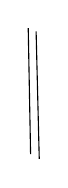
\begin{tikzpicture}\draw (0,0) -- (0.03,-1.6);\draw (0.10,-0.04) -- (0.14,-1.66);\end{tikzpicture}}}
La conjecture qui se présente tout de suite, c'est que ces deux revêtements proétales sont isomorphes -- l'isomorphisme entre les deux \unsure{est} alors unique.


\deleted{\unsure{Et}} C'est le moment de déterminer les classes d'isomorphie des \unsure{classes} de scindages de \inserted{l'ext. $\widetilde{\mathcal M}\unsure{\simeq}\mathcal M_{0,3}/[\widehat\Pi_{0,3},\widehat\Pi_{0,3}]$ de} $\Gamma=\Gamma_{\mathbb Q}\times\mathfrak S_3$ par $M^{\wedge}$, on a par la suite exacte associée à la suite spectrale de Hochschild

$(294)$\quad
\diagram{\begin{tikzcd}[ampersand replacement=\&,column sep=small]
0\arrow[r,dash]\&H^1(\Gamma_{\mathbb Q},H^0(\deleted{\unsure{\widetilde\Gamma}}\mathfrak S_3,\widehat M))\arrow[r,dash]\&H^1(\unsure{\Gamma},\widehat M)\arrow[r,dash]\&H^0(\Gamma_{\mathbb Q},H^1(\mathfrak S_3,\widehat M))\arrow[d]\\
\&\&\&H^2(\Gamma_{\mathbb Q},H^0(\mathfrak S_3,M))
\end{tikzcd}}

Or on a vu que
\[
(295)\qquad H^0(\mathfrak S_3,\widehat M)=0
\qquad(\text{\unsure{et} }\overline{\mathrm m}\ H^0(\unsure{L_\rho|L_j},\unsure{\widehat M|\overline M})=0)
\]
\margin{donc $H^1(\Gamma,\widehat M)\simeq H^0(\Gamma_{\mathbb Q},H^1(\mathfrak S_3,\widehat M))$}
\deleted{\unsure{Et}} Calculons d'autre part
\[
H^1(\mathfrak S_3,\widehat M)=H^1(\mathfrak S_3,M)\otimes_{\mathbb Z}\widehat{\mathbb Z},
\]

\margin{135}

% Archive printed footer (not manuscript):
% 135
% https://grothendieck.umontpellier.fr
% Université de Montpellier, UMR CNRS 5149, Case courrier 051, Place Eugène Bataillon
% 34095 Montpellier cedex 5 - France
\scanpage{137}
\mspage{716}

ce qui nous \unsure{ramène} à calculer
\[
H^1(\mathfrak S_3,M)\quad ?
\]
Mais l'étude faite de l'extension $\unsure{\mathfrak G}^+/\mu_{\unsure{\mathfrak G|G}}$ de $\mathfrak S_3$ par $M$ -- qui nous a montré que cette extension était scindée, et que deux scindages étaient conjugués par un unique élément de $M$, nous donne en fait
\[
(296)\qquad
\left\{\begin{array}{ll}
H^0(\mathfrak S_3,M)=H^1(\mathfrak S_3,M)=0&\text{d'où}\\
H^0(\mathfrak S_3,\unsure{\widehat M|\overline M})=H^1(\mathfrak S_3,\unsure{\widehat M|\overline M})=0&
\end{array}\right.
,
\]
d'où finalement, grâce à $(295)$, la relation triomphale
\[
(297)\qquad\boxed{H^1(\Gamma_{\mathbb Q}\times\mathfrak S_3,\widehat M)=0}\qquad !
\]

On trouve donc -- à nouveau contre toute attente, je l'avoue ! -- le

\uline{Théorème}\quad Il existe un \deleted{pro}revêtement
\margin{\figure{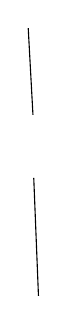
\begin{tikzpicture}\draw (0,0) -- (0.06,-1.1);\draw (0.07,-1.9) -- (0.13,-3.4);\end{tikzpicture}}}
proétale \deleted{$\unsure{X|Z}$} $U_\infty$ de $(U_{0,3\,\mathbb Q},\mathfrak S_3)$\inserted{$=M'_{1,1\,\mathbb Q}$}, ayant la propriété suivante : L'image inverse \inserted{$\overline U_\infty$} de $U_\infty$ sur $U_{0,3\,\overline{\mathbb Q}}$ (\deleted{\unsure{sans}}\inserted{\unsure{oubliant}} op. de $\mathfrak S_3$) est ``le'' revêtement abélien universel de $U_{0,3\,\overline{\mathbb Q}}$. Pour deux tels revête-

\margin{136}

% Archive printed footer (not manuscript):
% 136
% https://grothendieck.umontpellier.fr
% Université de Montpellier, UMR CNRS 5149, Case courrier 051, Place Eugène Bataillon
% 34095 Montpellier cedex 5 - France
\scanpage{138}

ments proétales de $(U_{0,3\,\mathbb Q},\mathfrak S_3)=M'_{1,1\,\mathbb Q}$, il existe un unique isomorphisme de l'un sur l'autre.

Nous avons obtenu l'existence de \uline{deux} façons : par la tour de Fermat, et par la théorie générale du \S\,$49$ \uline{III}, appliquée au cas présent -- ce qui nous donne un $U_\infty$ et un $U'_\infty$, chacun décrit à isom unique près ! Le th. d'unicité résulte du petit calcul précédent -- j'avais peur du ``gros'' \deleted{$\unsure{H^1(\Gamma_{\mathbb Q},\widehat M)\simeq H^1(\Gamma}$}
\[
H^1(\Gamma_{\mathbb Q},\widehat M)\simeq
M\otimes_{\mathbb Z}\underbrace{H^1(\Gamma_{\mathbb Q},T_{\unsure{\infty|*}}(G_m))}_{\widehat{\mathbb Q^{*}}},
\]
mais finalement c'est la nullité de $H^{\unsure{i}}(\mathfrak S_3,M)$ pour $i=0,1$ qui implique (sans rien connaître sur $\Gamma_{\mathbb Q}$ !) celle de $H^1(\Gamma_{\mathbb Q}\times\mathfrak S_3,\widehat M)$, qui assure l'unicité qu'il nous fallait.

\margin{137}

% Archive printed footer (not manuscript):
% 137
% https://grothendieck.umontpellier.fr
% Université de Montpellier, UMR CNRS 5149, Case courrier 051, Place Eugène Bataillon
% 34095 Montpellier cedex 5 - France
\scanpage{139}
\mspage{717}

\deleted{Car} Le théorème précédent élucide complètement, il me semble, la signification arithmético-géométrique (en termes de la tour de Fermat) de l'homomorphisme ((218) p.~695')
\[
\mathcal M=N_{1,1}^{\text{ét}}\longrightarrow G_{\rho,\sigma}\simeq\widehat{\mathbb Z}^{*}\mathbin{.}\unsure{\mathfrak G_{\bullet}^{+\wedge}}
\]
obtenu dans la section 11°) par voie purement algébrique --- ou du moins celui de l'homomorphisme un peu plus faible
\[
\mathcal M\longrightarrow\overbrace{G_{\rho,\sigma}/\mu_{\unsure{\mathfrak G}}}^{\inserted{G_{\rho,\widetilde{\sigma}}\overset{\mathrm{dfn}}{=}}}\simeq\widehat{\mathbb Z}^{*}\mathbin{.}\unsure{\mathfrak G^{+\wedge}/\mu_{\mathfrak G}}
\]
qui se factorise \deleted{par} en un hom
\[
\underbrace{\widetilde{\mathcal M}}_{\inserted{\text{noté }\mathcal M\text{ dans les pages précédentes}}}\overset{\mathrm{dfn}}{=}\mathcal M/(\mu_{\mathcal M}=\unsure{\mu_{\mathfrak G_\bullet}})\longrightarrow G_{\rho,\widetilde{\sigma}}
\qquad\text{extension de }\widetilde\Gamma=\widehat{\mathbb Z}^{*}\times\mathfrak S_3\text{ par }M^\wedge.
\]

Le passage de $G_{\rho,\sigma}^{\deleted{\unsure{\sim}}}$ à $G_{\rho,\widetilde{\sigma}}$, du point de vue actuel, avait comme rôle essentiel (a posteriori !) de fournir une extension par $M^\wedge$ (jouant le rôle d'une composante neutre) d'un groupe opérant \uline{fidèlement} sur $M^\wedge$, ce qui n'était pas le cas de l'ext. $G_{\rho,\sigma}$ de $\widehat{\mathbb Z}^{*}\times H^+$ par $M^\wedge$, puisque le \deleted{\unsure{élément}} \inserted{centre $\mu_{H^+}=\{1,\unsure{\omega_{H^+}}\}$ \deleted{\unsure{$H^+$}} de $H^+$} opérait trivialement.
\margin{138}

% Archive printed footer (not manuscript):
% 138
% https://grothendieck.umontpellier.fr
% Université de Montpellier, UMR CNRS 5149, Case courrier 051, Place Eugène Bataillon
% 34095 Montpellier cedex 5 - France
\scanpage{140}

Ceci, joint aux relations
\[
H^0(\widehat{\mathbb Z}^{*}\times\mathfrak S_3,\widehat M)=H^1(\widehat{\mathbb Z}^{*}\times\mathfrak S_3,\widehat M)=0,
\]
permettait d'interpréter le groupe $G_{\rho,\widetilde\sigma}$ comme un groupe de transformations sur l'ens $E$ de ses propres scindages, ce qui permettait d'interpréter l'hom $\mathcal M\to G_{\rho,\widetilde\sigma}$ (ou $\widetilde{\mathcal M}\to G_{\rho,\widetilde\sigma}$) comme une \deleted{\unsure{ho}} \uline{opération} de $\mathcal M$ \deleted{\unsure{de $H$}} (ou mieux, \deleted{de $\unsure{\widetilde{\mathcal M}}$}\inserted{de $\widetilde{\mathcal M}=\pi_1(U_{0,3\mathbb Q},\mathfrak S_3)=\pi_1(M'_{1,1\mathbb Q})$} sur $E$), correspondant donc à un revêtement \inserted{proétale} de $(U_{0,3\mathbb Q},\mathfrak S_3)\simeq M'_{1,1\mathbb Q}$ --- et ce revêtement n'est autre que le prorevêtement de Fermat.

Il restait à interpréter de façon analogue l'hom $\boxed{\mathcal M=N_{1,1}\longrightarrow G_{\rho,\sigma}}$, s'insérant dans l'hom de suites exactes
\[
\tag{298}
\diagram{\begin{tikzcd}[ampersand replacement=\&,column sep=small,row sep=large]
1\arrow[r]\&\begin{gathered}\mu_{\mathcal M}\\\Vert\\(\{1,\omega\})\end{gathered}\arrow[r]\arrow[d,"\simeq"]\&\begin{gathered}\mathcal M\\\Vert\\(N_{1,1})\end{gathered}\arrow[r]\arrow[d]\&\begin{gathered}\widetilde{\mathcal M}\\\Vert\\(N'_{1,1}=\unsure{\mathcal M_{0,3}})\end{gathered}\arrow[r]\arrow[d]\&1\\
1\arrow[r]\&\begin{gathered}\mu_G\\\Vert\\\{1,\omega\}\end{gathered}\arrow[r]\&G_{\rho,\sigma}\arrow[r]\&G_{\rho,\widetilde\sigma}\arrow[r]\&1
\end{tikzcd}},
\]
\deleted{Pour} qui permet d'interpréter d'ailleurs $\mathcal M$, en tant qu'extension centrale de $\widetilde{\mathcal M}$
\margin{139}

% Archive printed footer (not manuscript):
% 139
% https://grothendieck.umontpellier.fr
% Université de Montpellier, UMR CNRS 5149, Case courrier 051, Place Eugène Bataillon
% 34095 Montpellier cedex 5 - France
\scanpage{141}
\mspage{718}

par $\mu$, comme image inverse de l'extension $G_{\rho,\sigma}$ de $G_{\rho,\widetilde\sigma}$ par $\mu$, par l'homomorphisme $\widetilde{\mathcal M}\to G_{\rho,\widetilde\sigma}$ précédent. Il y a une analogie frappante avec ce qui s'était passé, d'ailleurs, quand on était parti \unsure{de} (au \S~48, et \unsure{dans|des} certains développements qui l'ont précédé) du groupe quotient (``du type Lie'') $\unsure{\mathrm{SL}(2,\widehat{\mathbb Z})'}$ de $\unsure{\mathfrak G_{0,3}^{+\wedge}}$, pour construire un hom
\[
\deleted{\unsure{\mathcal M}}\qquad \mathcal M_{0,3}\longrightarrow\mathrm{GL}(2,\widehat{\mathbb Z})/\{\pm1\}
\]
d'où il nous a été possible de reconstituer \deleted{$\unsure{\mathcal M}$} l'ext. $\mathcal M=N_{1,1}$ de $\mathcal M_{0,3}$ par $\mu$ justement comme l'image inverse de l'extension $\mathrm{GL}(2,\widehat{\mathbb Z})$ de $\mathrm{GL}(2,\widehat{\mathbb Z})/\{\pm1\}$ par $\mu=\{\pm1\}$. Du pt de vue actuel où j'essaye d'expliciter autant que possible des aspects arithmético-géométriques en termes d'automorphismes des groupes à lacets \inserted{profinis} $\Pi_{0,\unsure{3|2}}^\wedge$ --- le fait remarquable, c'est que les deux
\margin{140}

% Archive printed footer (not manuscript):
% 140
% https://grothendieck.umontpellier.fr
% Université de Montpellier, UMR CNRS 5149, Case courrier 051, Place Eugène Bataillon
% 34095 Montpellier cedex 5 - France
\scanpage{142}

extensions de $\widetilde{\mathcal M}$ par $\mu$, sortant de calculs en apparence assez différents, soient canoniquement isomorphes.

Je \unsure{présume|pense} qu'une explication générale de ce fait \unsure{n'offre} aucune difficulté, dans le contexte actuel --- du fait que dans les deux cas, le \inserted{bi-}\unsure{revêtement} de $\unsure{\mathrm{GL}}(2,\widehat{\mathbb Z})/\pm1$ resp de $G_{\rho,\widetilde\sigma}$ provenait du fait que j'étais parti d'un groupe quotient ($\mathrm{SL}(2,\widehat{\mathbb Z})$ ou $\unsure{\mathfrak G^{+\wedge}}$) \uline{non pas} de $\unsure{\mathfrak G_{0,3}^{+\wedge}}\simeq\mathrm{SL}(2,\mathbb Z)^\wedge/\pm1$, mais de $\mathrm{SL}(2,\mathbb Z)^\wedge\simeq N_{1,1}$ lui-$\overline{\mathrm m}$.

Si on cherche malgré tout une interprétation (genre ``tour de Fermat'') de l'hom $\mathcal M\to G_{\rho,\sigma}$, il faudrait interpréter $G_{\rho,\sigma}$ \inserted{(comme \unsure{l'était} $G_{\rho,\widetilde\sigma}$)} comme un groupe d'automorphismes d'une ``fibre type'' ``pas trop grosse'' --- la difficulté étant d'inventer quelque chose sur quoi \unsure{ça|il} opère de façon non triviale.
\margin{141}

% Archive printed footer (not manuscript):
% 141
% https://grothendieck.umontpellier.fr
% Université de Montpellier, UMR CNRS 5149, Case courrier 051, Place Eugène Bataillon
% 34095 Montpellier cedex 5 - France
\scanpage{143}
\mspage{719}

Interprétant $\mathcal M_{0,3}=N'_{1,1}$ comme $\pi_1(M'_{1,1})$, où $M'_{1,1}$ est le schéma modulaire/$\mathbb Q$ des courbes elliptiques à symétrie près, on voit que la tour de Fermat revient à ceci : sur tout schéma de base $S$ (disons \inserted{\uline{de car. 0}}) et \unsure{tte|tt} quasi-courbe elliptique \inserted{\deleted{$\unsure{E}$}$\widetilde X$} sur $S$, considérons le revêtement étale de degré trois $S'$ de $S$ correspondant (\inserted{des} ``pts d'ordre 2 de $\widetilde X$''), \deleted{posons} soit
\[
\tag{299}
\deleted{\unsure{M_2}}\quad M_0(\widetilde X/\unsure{S|B})\overset{\mathrm{dfn}}{=}p_*(\mathbb Z_{\unsure{S'|B'}})/\mathbb Z_S
\]
le $\mathbb Z$-module constant tordu libre de rang \deleted{trois}\inserted{deux} correspondant, et considérons
\[
\tag{300}
\deleted{\unsure{M_2}}\quad M_1(\widetilde X/S)\overset{\mathrm{dfn}}{=}M_0(\widetilde X/S)\otimes_{\mathbb Z}\underbrace{\unsure{\widehat{\mathbb Z}(1)}}_{\inserted{\begin{gathered}\Vert\,\mathrm{dfn}\\T_\infty(\mathbb G_m)\end{gathered}}},
\]
qui est un \deleted{pro}groupe proétale sur $S$, un syst de coefficients locaux\unsure{;} (au sens large) à $\widehat{\mathbb Z}^{2}$. \deleted{Ceci posé,}\inserted{Bien} sûr, $M_1(\widetilde X/S)$ dépend \unsure{fonctoriellement} de $\widetilde X/S$ pour iso et images inverses (on a une section cartésienne d'une cat. fibrée ad-hoc $\ldots$). Ceci posé,
\margin{142}

% Archive printed footer (not manuscript):
% 142
% https://grothendieck.umontpellier.fr
% Université de Montpellier, UMR CNRS 5149, Case courrier 051, Place Eugène Bataillon
% 34095 Montpellier cedex 5 - France
\scanpage{144}

la donnée de la ``tour de Fermat'' équivaut à la donnée, pour $\forall\,\widetilde X/S$ comme dessus, d'un torseur
\[
\tag{301}
F_\infty(\widetilde X/S)\quad\text{torseur sur }S\text{ sous }M_1(\widetilde X/S),
\]
\margin{pour une construction géométrique cf (320) p. 724}
compatible aux iso. et \unsure{chgts} de base.

Le théorème précédent dit essentiellement qu'un tel $F_\infty(\widetilde X/S)$ existe, et est unique à iso. unique près, en exigeant de plus que l'hom naturel
\diagram{\begin{tikzcd}[ampersand replacement=\&]
\Pi_{0,3}^{\wedge}\arrow[r] \& M^{\wedge}
\end{tikzcd}}
associé à une telle donnée $F_\infty$ soit l'hom canonique $\ldots$.

Soit d'autre part $X$ une courbe elliptique relative au dessus d'une base $S$ de car. 0, et soit $S'\subset X$ le sous-schéma fermé, étale de degré 3 sur $S$, correspondant aux pts d'ordre 2. Considérons la \unsure{jacobienne généralisée} de $X$ déduite de cette multisection, soit $\mathcal J^0$ sa partie de degré 0, on a donc

\margin{143}

% Archive printed footer (not manuscript):
% 143
% https://grothendieck.umontpellier.fr
% Université de Montpellier, UMR CNRS 5149, Case courrier 051, Place Eugène Bataillon
% 34095 Montpellier cedex 5 - France
\scanpage{145}
\mspage{720}

une suite exacte
\[
\tag{302}
\diagram{\begin{tikzcd}[ampersand replacement=\&]
1\arrow[r] \& \mathcal J_0^0\arrow[r,dash]\arrow[d,phantom,"\rotatebox{90}{$\simeq$}" description] \& \mathcal J^0\arrow[r] \& X\arrow[r,dash] \& 1\\
\& \mathbb G_m\otimes_{\mathbb Z}M_0
\end{tikzcd}}
\]
où $M_0=M_0(X/S)$ est défini plus haut (299). On en déduit une suite exacte
\[
\tag{303}
\diagram{\begin{tikzcd}[ampersand replacement=\&]
1\arrow[r] \& M_1\arrow[r]\arrow[d,equal] \& T_\infty(\mathcal J^0)\arrow[r] \& T_\infty(X)\arrow[r,dash] \& 1\\
\& M_0\otimes_{\mathbb Z}T_\infty(\mathbb G_m)
\end{tikzcd}}
\]
où
\[
\tag{\uline{304}}
T_\infty(G)=\varprojlim_n {}_nG
\]
est le système local des $\Pi_1$ du schéma en groupes lisse comm. \inserted{à fibres connexes} sur $S$. Donc la donnée d'un torseur sous $M_1$ équivaut à la donnée d'un torseur sous $T_{\unsure{\infty|\alpha}}(\mathcal J^0)$, muni d'une section du torseur associé \unsure{du|de} groupe $T_\infty(X)$.
\unsure{Y-a-t-il|Y a-t-il} une description remarquable du torseur de Fermat $F_\infty(X/S)$, en termes de la géométrie de la courbe elliptique relative $X/S$ ?

\margin{144}

% Archive printed footer (not manuscript):
% 144
% https://grothendieck.umontpellier.fr
% Université de Montpellier, UMR CNRS 5149, Case courrier 051, Place Eugène Bataillon
% 34095 Montpellier cedex 5 - France
\scanpage{146}

$14^\circ)$ Relation aux jacobiennes généralisées.

Considérons la ``jacobienne généralisée'' de
\[
\inserted{U_{0,3}={}}U_{0,3\,\deleted{\unsure{\mathbb Q}}\inserted{\mathbb Z}}
=\deleted{\unsure{\mathbb A_{\mathbb Q}}}\mathbb P^1_{\deleted{\unsure{\mathbb Q}}\inserted{\mathbb Z}}
-\{0,1,\infty\}_{\deleted{\unsure{\mathbb Q}}\inserted{\mathbb Z}},
\]
c'est donc un schéma en groupes $\mathcal J^*_{U_{0,3}}=\mathcal J^*$, \unsure{augmenté|s'envoyant} vers $\mathbb Z$, s'insérant dans la suite exacte
\[
\tag{305}
\diagram{\begin{tikzcd}[ampersand replacement=\&]
1\arrow[r] \& \mathcal J^0\arrow[r]\arrow[d,phantom,"\rotatebox{90}{$\simeq$}" description] \& \mathcal J^*\arrow[r,"\deg"] \& \mathbb Z_{\inserted{S_0}\deleted{\unsure{\mathbb Q}}}\arrow[r] \& 1\\
\& \mathbb G_{mS_0}\otimes_{\mathbb Z}M_{\unsure{0|\mathbb Z}}
\end{tikzcd}},
\]
\margin{\uline{NB} $S_0\overset{\unsure{\mathrm{df}|\mathrm{dfn}}}{=}\operatorname{Spec}\mathbb Z$}
et muni d'un \deleted{homo}morphisme canonique
\[
\tag{306}
\diagram{\begin{tikzcd}[ampersand replacement=\&]
\varphi:\ U_{0,3\,\deleted{\unsure{\mathbb Q}}\inserted{\mathbb Z}}\arrow[r] \&
\underbrace{\mathcal J^1}_{\substack{\text{sous-schéma de }\mathcal J^*\\\text{image inverse de}\\\text{la section }1\text{ de }\mathbb Z_{S_0}}}
\end{tikzcd}}
\]
Les opérations de $\mathfrak S_3$ sur $U_{0,3}$ définissent par fonctorialité des opérations de $\mathfrak S_3$ sur $\mathcal J^*$, compatibles avec la structure d'extension (305), et telles que (306) commute aux opérations de $\mathfrak S_3$.
Notons que $\mathcal J^1$ est un $\mathcal J^0$-torseur et

\margin{145}

% Archive printed footer (not manuscript):
% 145
% https://grothendieck.umontpellier.fr
% Université de Montpellier, UMR CNRS 5149, Case courrier 051, Place Eugène Bataillon
% 34095 Montpellier cedex 5 - France
\scanpage{147}
\mspage{721}

même un $(\mathfrak S_3,\mathcal J^0)$-torseur (un $\mathcal J^0$-torseur sur lequel $\mathfrak S_3$ opère de façon compatible avec ses op. sur $\mathcal J^0$), donc classifié par un élément de $H^1(S_0,\mathfrak S_3;\mathcal J^0)$. Or je présume qu'on a
\[
\tag{307}
H^0(S_0,\mathfrak S_3,\mathcal J^0)=H^1(S_0,\mathfrak S_3,\mathcal J^0)=0
\]
(où
\[
\tag{308}
\left\{\begin{aligned}
S_0&=\operatorname{Spec}\mathbb Z,\quad \mathcal J^0=\mathbb G_m\times_{\mathbb Z}M\simeq\mathbb G_m^{\{0,1,\infty\}}/\mathrm{diag}\\
&\simeq\operatorname{Ker}\left(\diagram{\begin{tikzcd}[ampersand replacement=\&,column sep=small]
\mathbb G_m^{\{0,1,\infty\}}\arrow[r] \& \mathbb G_m^{\deleted{\unsure{\{0,1,\infty\}}}}\\
(x_0,x_1,x_\infty)\arrow[r,mapsto] \& \substack{\inserted{x_0\cdot x_1\cdot x_\infty}\\\deleted{\unsure{(x_1x_\infty^{-1},x_\infty x_0^{-1},x_0x_1^{-1})}}}
\end{tikzcd}}\right)
\end{aligned}\right.
\]
\margin{Attention, ce dernier isom. est obtenu \unsure{via}
\diagram{\begin{tikzcd}[ampersand replacement=\&]
(x_0,x_1,x_\infty)\arrow[r,mapsto] \& (x_1x_\infty^{-1},x_\infty x_0^{-1},x_0x_1^{-1})
\end{tikzcd}}, qui commute à $\mathfrak S_3^+$, mais \unsure{non|pas} à $\mathfrak S_3$ tout entier}

On a en effet
\[
\begin{aligned}
H^0(S_0,\mathfrak S_3;\mathcal J^0)&\simeq\left\{(x_0,x_1,x_\infty)\in\mathbb Z^{*\{0,1,\infty\}}\ \middle|\ \begin{array}{l}x_0x_1x_\infty=1\\(x_0,x_1,x_\infty)\text{ inv. par }\mathfrak S_3\end{array}\right\}\\
&=\{(x,x,x)\mid x\in\mathbb Z^{*\{0,1,\infty\}},\quad x^3=1\}\\
&=1
\end{aligned}
\]
\margin{Calcul \unsure{correct}, car il \unsure{repose sur cet} $\mathfrak S_3^+$-isom. qui n'est pas un $\mathfrak S_3$-isom., \unsure{il semble ici qu'être|il semble n'y être} besoin de $H^0(S,\mu_3)=1$, alors qu'un calcul déjà fait des \unsure{scindages} d'extensions (cf. 720) montre que $\unsure{S}$ -- sur \uline{toute} \uuline{base}
\diagram{\begin{tikzcd}[ampersand replacement=\&,column sep=small]
H^0(S,\mathfrak S_3,\mathcal J^0)\arrow[d,equal]\arrow[r,phantom,"\simeq"] \& H^1(\deleted{\unsure{S,}}\mathfrak S_3;H^0(\unsure{S|S_0},\mathcal J^0))\simeq0\quad\unsure{\Leftarrow}\\
H^0(\mathfrak S_3,H^0(S,\mathcal J^0))
\end{tikzcd}}}

(\unsure{la} seule racine \deleted{\unsure{de}} cubique de 1 dans $\mathbb Z$ (ou $\overline{\mathrm m}$ dans $\mathbb Q$) est 1. Cela établit la première relation (307). Pour la seconde, on utilise la suite spectrale

\margin{146}

% Archive printed footer (not manuscript):
% 146
% https://grothendieck.umontpellier.fr
% Université de Montpellier, UMR CNRS 5149, Case courrier 051, Place Eugène Bataillon
% 34095 Montpellier cedex 5 - France
\scanpage{148}

\diagram{\begin{tikzcd}[ampersand replacement=\&]
H^{\unsure{*|n}}(S_0,\mathfrak S_3;\mathcal J^0) \&
\overset{\inserted{E_2^{pq}=}}{H^p(\mathfrak S_3,\uline{H}^{q}(S_0,\mathcal J^0))}\arrow[l,Rightarrow]
\end{tikzcd}}
qui donne la suite exacte
\diagram{\begin{tikzcd}[ampersand replacement=\&,column sep=small]
0\arrow[r] \& H^1(\mathfrak S_3,H^0(S_0,\mathcal J^0))\arrow[r,"\unsure{\deleted{\simeq}|\simeq}"] \& H^1(S_0,\mathfrak S_3;\mathcal J^0)\arrow[r] \& H^0(\mathfrak S_3,H^1(S_0,\mathcal J^0))\arrow[d]\arrow[dl,equal]\\
\& \& \bigl(H^{\unsure{0|q}}(\mathfrak S_3,M_{\unsure{0}}\otimes_{\mathbb Z}H^1(S_0,\mathbb G_m))\bigr) \& H^2(\mathfrak S_3,H^0(S_0,\mathcal J^0))
\end{tikzcd}}

Or on a
\[
H^1(S_0,\mathcal J^0)\simeq H^1(S_0,\mathbb G_m^2)\simeq\operatorname{Pic}(\unsure{S|S_0})^2=0
\]
\margin{\uline{NB} on n'a \uline{pas} besoin de la relation $\operatorname{Pic}(S)=0$}
donc il vient
\[
H^1(S_0,\mathfrak S_3;\mathcal J^0)\simeq H^1(\mathfrak S_3,\underbrace{H^0(S_0,\mathcal J^0)}_{\substack{\deleted{(\mathbb Z^*)^{\{0,1,\infty\}}/\mathbb Z^*}\\\deleted{\simeq\mathbb Z^*\otimes_{\mathbb Z}M_0}}})
\]

Mais en fait, les calculs faits par ailleurs montrent qu'on a
\[
\tag{309}
H^0(\mathfrak S_3,M_{\unsure{0|\alpha}}\otimes_{\mathbb Z}\unsure{I|I_0})=H^1(\mathfrak S_3,M_{\unsure{0|\alpha}}\otimes_{\mathbb Z}I)=0
\]
quel que soit le $\mathbb Z$-module $I$ (p. ex. $I=\unsure{J^0|\mathcal J^0}(S)$, $S$ un schéma \unsure{quelc.|quelq.}, \inserted{ou $I=H^1(S,\mathbb G_m)=\operatorname{Pic}(S)$}), d'où finalement,
\[
\tag{\unsure{310}}
H^0(\unsure{\deleted{S_0}|S},\mathfrak S_3;\mathcal J^0)\simeq H^1(S,\mathfrak S_3,\mathcal J^0)=0
\]
pour $\forall$ schéma $S$. On trouve ainsi :

\margin{147}

% Archive printed footer (not manuscript):
% 147
% https://grothendieck.umontpellier.fr
% Université de Montpellier, UMR CNRS 5149, Case courrier 051, Place Eugène Bataillon
% 34095 Montpellier cedex 5 - France
\scanpage{149}
\mspage{722}

\uline{Proposition} Soit \deleted{$\unsure{\mathcal J}$}
$\mathcal J^0=\mathbb G_m^{\{0,1,\infty\}}/\underbrace{\mathbb G_m}_{\mathrm{diag.}}\simeq\mathbb G_m\otimes_{\mathbb Z}\unsure{M_0|M}$
Alors pour $\forall$ $(\mathfrak S_3,\mathcal J^0)$-torseur sur une base $S$ quelconque, il existe une unique trivialisation de celui-ci, i.e une unique section, invariante par les opérations de $\mathfrak S_3$.

\uline{Corollaire 1} Sur toute base $S$, il existe un unique morphisme
\[
(311)\qquad
\diagram{\begin{tikzcd}[ampersand replacement=\&]
\psi:U_{0,3\,S} \arrow[r] \& \mathcal J^0_S
\end{tikzcd}}
\]
qui soit compatible avec les opérations de $\mathfrak S_3$, et qui (via l'hom
$\mathcal J^*_S\longrightarrow\mathcal J^0_S$ \unsure{qui|que} \unsure{le|la} \unsure{factorise}, par la propriété universelle des \unsure{jacobiens} généralisés) induise l'hom
$\underset{\inserted{\mathcal J^*_S}}{\mathcal J^0_S}-\mathcal J^0_S$ identique.

\margin{\uline{NB} Avec les notations de \unsure{695}, on a $U_{0,3\,S}\simeq(U_1)_S$, où $U_1\subset\mathbb G_m^3/\mathbb G_m$ est \unsure{défini} par
\[
(312)\qquad
U_1=\{(x_0,x_1,x_\infty)\in\prod^{\{0,1,\infty\}}\mathbb G_m\mid x_0+x_1+x_\infty=\unsure{0}\}
\quad\mathrm{mod}\ \mathrm{diag}_3\mathbb G_m.
\]}

\uline{Corollaire 3} Soit $Y$ un schéma de

\margin{148}

% Archive printed footer (not manuscript):
% 148
% https://grothendieck.umontpellier.fr
% Université de Montpellier, UMR CNRS 5149, Case courrier 051, Place Eugène Bataillon
% 34095 Montpellier cedex 5 - France
\scanpage{150}

\unsure{Brauer}-Séveri sur $S$, de dim relative $1$ (i.e. une forme de $\mathbb P^1_S$), muni d'un sous-schéma \inserted{fermé} $S'\subset Y$, étale de degré $3$ sur $S$, et soit \deleted{$\unsure{X}$} $U=Y\setminus S'$, $\mathcal J^*_{U/S}$ le jacobien généralisé, de sorte qu'on a
\[
(313)\qquad
\diagram{\begin{tikzcd}[ampersand replacement=\&,column sep=1.5em,row sep=.5em]
1 \arrow[r,no head] \& \mathcal J^0_{U/S} \arrow[r,no head] \arrow[d,phantom,"\unsure{\wr}" description] \& \mathcal J^*_{U/S} \arrow[r,no head] \& \mathbb Z_S \arrow[r,no head] \& 1 \\
\& \mathbb G_m\otimes_{\mathbb Z}\unsure{M_0}(S'/S) \& \& \&
\end{tikzcd}}
\]
où $\unsure{M_0}(S'/S)\simeq\unsure{p_*|\rho_*}(\mathbb Z_{S'})/\underbrace{\mathbb Z_S}_{\mathrm{diag}}$ est le $S$-schéma \inserted{en \deleted{groupes} \inserted{$\mathbb Z$-modules}} (loc. $\unsure{\overline{\mathrm{isom.}}}$ à $\mathbb Z^{\unsure{2}}$, déduit de $\unsure{M_{0\,S}}$ en le tordant (via action de $\mathfrak S_3$) par le \deleted{fibré principal} \inserted{$\mathfrak S_3$-torseur sur $S$} associé à $S'$.

Il existe alors un unique morphisme
\[
(\unsure{314})\qquad
\diagram{\begin{tikzcd}[ampersand replacement=\&]
\psi:U \arrow[r] \& \mathcal J^0_{U/S}
\end{tikzcd}}
\]
commutant à \deleted{$\uline{\operatorname{Aut}}$} l'action de $\uline{\operatorname{Aut}}(S'/S)\xleftarrow{\sim}\uline{\operatorname{Aut}}_S(Y,S')$, et induisant (par la propriété universelle) \deleted{\unsure{un}} l'hom. \unsure{composé}
\[
\diagram{\begin{tikzcd}[ampersand replacement=\&]
\mathcal J^0_{U/S} \arrow[r,hook] \& \mathcal J^*_{U/S} \arrow[r,"\widetilde\psi"] \& \mathcal J^0_{U/S}
\end{tikzcd}}
\]
qui soit l'identité.

\margin{149}

% Archive printed footer (not manuscript):
% 149
% https://grothendieck.umontpellier.fr
% Université de Montpellier, UMR CNRS 5149, Case courrier 051, Place Eugène Bataillon
% 34095 Montpellier cedex 5 - France
\scanpage{151}
\mspage{723}

Explicitons l'\unsure{\uline{hom}omorphisme|\uline{hom}orphisme}
\[
(315)\qquad
\diagram{\begin{tikzcd}[ampersand replacement=\&,column sep=2em,row sep=.9em]
U_{0,3}=\mathbb P^1\setminus\{0,1,\infty\}_{S_0}
  \arrow[r,hook,"\psi"] \arrow[d,equal]
\& \underbrace{\mathbb G_m^{\{0,1,\infty\}}/\mathbb G_m}_{\unsure{\mathcal J^0}}
\\
\begin{gathered}
\deleted{\{z\in\unsure{\Gamma}\mathbb G_m\mid z-1\ \mathrm{inv}\}}\\
\unsure{(}\mathbb G_m\setminus\{1\}\unsure{)}_{S_0}
\simeq\{z\in\Gamma\mathbb G_m\mid z-1\ \mathrm{inv}\}
\end{gathered}
\& \begin{gathered}
\deleted{\unsure{\mathcal J^1}}\inserted{U_1=\{(x_0,x_1,x_\infty)^{\deleted{\unsure{\mathbb Z}}}
\in\Gamma\mathbb G_m^3/\mathbb G_m\mid}\\
\inserted{x_0+x_1+x_\infty=0\}}
\end{gathered} \arrow[u,hook]
\end{tikzcd}}
\]
\deleted{\unsure{il est}} isomorphisme de $U_{0,3}$ avec $U_1$ qui \deleted{\unsure{est} \unsure{prolonge}} correspond :
\[
(\unsure{316|314})\qquad
\left\{\begin{array}{l}
\diagram{\begin{tikzcd}[ampersand replacement=\&,column sep=2em,row sep=.5em]
\overline\psi:\unsure{\widehat U_{0,3}|\overline U_{0,3}} \arrow[r] \arrow[d,equal]
\& \widehat U_1\subset\mathbb P^2_{S_0} \arrow[d,equal]\\
\mathbb P^1_{S_0}
\& \{(x_0,x_1,x_\infty)\in\unsure{\widehat{\mathbb P}^2_{\unsure{S_0}}|\mathbb P^2_{S_0}}\mid x_0+x_1+x_\infty=0\}
\end{tikzcd}}\\[1em]
\overline\psi(0)=(0,1,-1)\\
\overline\psi(1)=(-1,0,1)\\
\overline\psi(\infty)=(1,-1,0)
\end{array}\right.\ ,
\]
il suffit de prendre
\[
(317)\qquad
\psi(z)=(-z,z-1,1)=(1,1/z-1,-1/z)
\inserted{=\left(\frac{-z}{z-1},1,\frac{1}{z-1}\right)}.
\]

Revenons maintenant à la donnée d'une courbe elliptique relative \inserted{$X$} sur $S$ modulo symétrie (correspondant à un morphisme
$S\longrightarrow\deleted{\unsure{\operatorname{Spec}}}\mathcal M'_{1,1}$).

\margin{150}

% Archive printed footer (not manuscript):
% 150
% https://grothendieck.umontpellier.fr
% Université de Montpellier, UMR CNRS 5149, Case courrier 051, Place Eugène Bataillon
% 34095 Montpellier cedex 5 - France
\scanpage{152}

On suppose $2$ inv. sur $S$, de sorte que la donnée de $X$ \inserted{modulo $\omega_X$} correspond, par le \unsure{tapis} de Legendre $X\mapsto(X/\deleted{\text{\unsure{modulo sym.}}}\inserted{\{1,\omega_X\}})$, à la donnée d'un $(Y,S')$ comme dessus, avec en \uline{plus} une section de $U=Y-S'$.

En fait, la donnée de $(Y,S')$ revient à la donnée de $S'$, \inserted{i.e d'un $\mathfrak S_3$-torseur} \deleted{$Y$ se récupère} $T$ sur $S$ --- et $Y$ se récupère à partir de \unsure{là|lui} comme le schéma tordu $T\wedge_{\mathfrak S_3}\mathbb P^1_S$ \deleted{$\unsure{\wedge_{\mathfrak S_3}}$ \unsure{et|ou}, $T\wedge_{\mathfrak S_3}\mathcal J^0_{(U_{0,3})_S}\simeq\unsure{\mathcal J^0}$}
donc
\[
U=Y\setminus S'\simeq(T\wedge_{\mathfrak S_3}\mathbb P^1_S)\setminus\underbrace{T\wedge_{\mathfrak S_3}\{0,1,\infty\}_S}_{S'}
\]
plongé canoniquement dans
\[
T\wedge_{\mathfrak S_3}\mathcal J^0_{(U_{0,3})_S}\simeq\mathcal J^0_{U/S}.
\]
Le plongement $U\subset\mathcal J^0_{U/S}$ peut s'interpréter aussi comme un morphisme canonique
\[
(318)\qquad
\diagram{\begin{tikzcd}[ampersand replacement=\&]
X \arrow[r] \& \mathcal J^0_{U/S}\underbrace{=\mathcal J^0_{0\,X/S}}_{\substack{\text{\unsure{avec|en} notations}\\\text{de p. }720}}
\end{tikzcd}}
\]
qui doit être aisé à caractériser \unsure{axiomatiq}

\margin{151}

% Archive printed footer (not manuscript):
% 151
% https://grothendieck.umontpellier.fr
% Université de Montpellier, UMR CNRS 5149, Case courrier 051, Place Eugène Bataillon
% 34095 Montpellier cedex 5 - France
% ===== LM_C4-153-171: first pass, with mechanical fixes =====
\scanpage{153}
\mspage{724}

\unsure{ment}, \deleted{\illegible{1}} ou à expliciter en termes de ``fonctions elliptiques'' \unsure{standard}.

Sans m'attarder sur une telle explicitation, et revenant \inserted{plutôt} au plongement correspondant
\diagram{%
(\unsure{318})\qquad
\begin{tikzcd}[ampersand replacement=\&,column sep=large]
U \arrow[r,hook] \& \mathcal J^0_{U/S}
\end{tikzcd}}
et à la section \unsure{marquée}
\[
(\unsure{319})\qquad e\in U(S)=H^0(S,\mathcal J^0_{U/S}),
\]
\inserted{on peut utiliser la tour d'isogénies}
\deleted{on peut utiliser l'hom. canonique}
\diagram{%
\deleted{(\unsure{314})}\qquad
\begin{tikzcd}[ampersand replacement=\&,column sep=large]
\deleted{H^0(S,\mathcal J^0_{U/S})} \arrow[r,phantom,"\deleted{\longrightarrow}"{description}] \& \deleted{H}
\end{tikzcd}}
\diagram{%
(\unsure{321})\qquad
\begin{tikzcd}[ampersand replacement=\&,column sep=large]
1 \arrow[r,dash] \& {}_n\mathcal J^0_{U/S} \arrow[r,hook] \& \mathcal J^0_{U/S} \arrow[r,"n.\mathrm{id}_{\mathcal J^0_{U/S}}"] \& \mathcal J^0_{U/S} \arrow[r,dash] \& 1
\end{tikzcd}}
(pour $n$ variable), i.e. l'isogénie universelle déduite par passage à $\varprojlim$ :
\diagram{%
(\unsure{322})\qquad
\begin{tikzcd}[ampersand replacement=\&,column sep=large,row sep=large]
1 \arrow[r,dash] \& T_\infty(\mathcal J^0_{U/S}) \arrow[r,dash] \arrow[d,phantom,"\rotatebox{90}{$\simeq$}"{description}] \& \widetilde{\mathcal J}^0_{U/S} \arrow[r,"p"] \arrow[d,phantom,"\rotatebox{90}{$\underset{\mathrm{def}}{=}$}"{description}] \& \mathcal J^0_{U/S} \arrow[r] \& 1 \\
\& T_\infty(\mathbb G_m)_S\otimes_{\mathbb Z}\unsure{M_0}(S'/S) \& \varprojlim_n\unsure{{}_n}(\mathcal J^0_{U/S}) \& \&
\end{tikzcd}}
pour déduire, par image inverse de $e$, un torseur sous $T_\infty(\mathcal J^0_{U/S})\simeq T_\infty(\mathbb G_m)_S\otimes_{\mathbb Z}\unsure{M_0}(S'/S)$.

Ceci posé, on aura (cf (301) p. 719')
\[
(323)\qquad F_\infty(\widetilde X/S)\simeq p^{-1}(e),\quad\text{le }T_\infty(\mathcal J^0_{U/S})\text{-torseur}
\]
\inserted{déduit de la section $e$ de $\mathcal J^0_{U/S}$ sur $S$.}
\margin{152}
\scanpage{154}

\uline{Remarque} La classe d'isomorphie du $T_\infty(\mathcal J^0_{U/S})$-torseur obtenu est un élément de $H^1(S,T_\infty(\mathcal J^0_{U/S}))$, image de l'élément $e$ de $H^0(S,\mathcal J^0_{U/S})$, par le morphisme canonique
\diagram{%
(324)\qquad
\begin{tikzcd}[ampersand replacement=\&,column sep=large]
H^0(S,\mathcal J^0) \arrow[r] \& H^1(S,T_\infty(\mathcal J^0))
\end{tikzcd},}
dont le noyau est formé du sous-groupe de $H^0(S,\unsure{\mathcal J})$ des éléments ``infiniment divisibles''. Dans le cas où $S$ est \inserted{\unsure{réduit et est}} de type fini sur $\mathbb Z$ -- p.ex. \inserted{réduit} de type fini sur $\mathbb Q$ -- on sait (et c'est \deleted{\unsure{un théorème}} ``élémentaire'') que ce noyau est réduit à zéro. Cela signifie donc que la section $e$ \inserted{de $\unsure{U}$ sur $S$} (i.e. le ``paramètre elliptique'' envisagé) est alors entièrement déterminée, quand on connaît
\margin{153}
\scanpage{155}
\mspage{725}

$1^{\circ})$ le \deleted{\illegible{1}} \unsure{trirevêtement|trivêtement} étale $S'$ de $S$ associé, correspondant aux pts d'ordre $2$ de $\widetilde X/S$ -- d'où $\mathcal J^0\unsure{=}\mathcal J^0_{U/S}\simeq\mathcal J^0_0{}_{\deleted{\unsure{S}}}(\widetilde X,S')$ -- et

$2^{\circ})$ le $T_\infty(\mathcal J^{\unsure{0}}_{\deleted{\unsure{U/S}}})$-torseur $\unsure{\mathbb F_\infty|F_\infty}(\widetilde X/S)$ ;
\margin{154}
\scanpage{156}

$15^{\circ})$ Interprétation de $\Gamma_{\mathbb Q}\longrightarrow N_\sigma^{\unsure{\leftrightarrows}}$.

Au n° $11^{\circ}$ nous avons introduit l'hom. canonique
\diagram{%
\begin{tikzcd}[ampersand replacement=\&,column sep=huge,row sep=large]
\mathcal M\overset{\mathrm{def}}{=}\mathcal N_{1,1}^{\text{ét}} \arrow[r] \arrow[d,phantom,"\cup"{description}] \& \mathcal M_{\rho,\sigma}^{\sim} \arrow[d,phantom,"\cup"{description}] \\
\mathcal M^! \arrow[r] \& \mathcal M_{\rho,\sigma}^{\sim\unsure{\leftrightarrows}}
\end{tikzcd}\qquad\text{cf (217) p. \unsure{695})}}
que nous avons ``décomposé'' en \deleted{plus d'} deux homomorphismes (en plus d'un hom. trivial
\diagram{%
\begin{tikzcd}[ampersand replacement=\&,column sep=large,row sep=large]
\mathcal M \arrow[r] \arrow[dr] \& N_\rho^{\sim}\simeq\widehat{\mathbb Z}^{\times} \\
\& \Gamma_{\mathbb Q}^{\text{ét}} \arrow[u,"\chi"']
\end{tikzcd}}
) en \uline{deux} hom.
\diagram{%
(\unsure{325})\qquad
\begin{tikzcd}[ampersand replacement=\&,column sep=huge,row sep=large]
\mathcal M \arrow[r] \arrow[d,phantom,"\cup"{description}] \& G_{\rho,\sigma}\simeq\widehat{\mathbb Z}^{*}.\unsure{\mathcal G}^{+\wedge} \arrow[d,phantom,"\unsure{\cup}"{description}] \\
\mathcal M^! \arrow[r] \& G_{\rho,\sigma}^{\unsure{\leftrightarrows}}\simeq\widehat{\mathbb Z}^{*}.M^\wedge
\end{tikzcd}\qquad\text{(cf (218))}}
et
\diagram{%
(\unsure{326})\qquad
\begin{tikzcd}[ampersand replacement=\&,column sep=large]
\Gamma_{\mathbb Q}^{\text{ét}} \arrow[r] \& N_\sigma^{\unsure{\leftrightarrows}\deleted{\unsure{\sim}}}\simeq\widehat{\mathbb Z}^{*}.\widehat{\mathbb Z}
\end{tikzcd}\qquad\text{(cf (219)).}}

Le premier hom. (\unsure{322}) a été caractérisé en termes \inserted{\unsure{arithmético-}}\deleted{\unsure{algébriques}}géométriques (pour ce qui est de sa restriction à $\mathcal N_{1,1}\subset\mathcal N_{1,1}^{\text{ét}}$ lui-même, et en réduisant mod $\mu_G$ pour trouver un hom
\diagram{%
(327)\qquad\deleted{\unsure{$\mathcal M_{0,3}$}}\qquad
\begin{tikzcd}[ampersand replacement=\&,column sep=large]
\mathcal M_{0,3} \arrow[r,dash] \& G_{\rho,\sigma}^{\sim}\overset{\mathrm{def}}{\simeq}G_{\rho,\sigma}/\mu_G
\end{tikzcd},}
dans la section $13^{\circ})$, via la tour des
\margin{155}
\scanpage{157}
\mspage{\unsure{725|726}}

courbes de Fermat. Du point de vue actuel, où on essaye d'expliciter la géométrie algébrique de \inserted{\unsure{ess.\textsuperscript{t}}} type fini sur $\mathbb Q$ en termes d'\unsure{autom.} de groupes profinis, on peut dire aussi, inversement, que nous sommes arrivés à ``décrire'' la tour des courbes de Fermat, via l'hom (327) construit ici ``à la force du poignet''.

Il resterait maintenant à trouver une explicitation arithmético-géométrique de l'hom \deleted{\unsure{(322)}} de $\Gamma_{\mathbb Q}$ \inserted{$\subset\Gamma_{\mathbb Q}^{\text{ét}}$} dans $\widehat{\mathbb Z}^{*}.\widehat{\mathbb Z}$, induit par (\unsure{326}).
Mais \deleted{\unsure{cet l'hom.}} utilisant le plongement
(\diagram{%
\begin{tikzcd}[ampersand replacement=\&,column sep=large]
N_\sigma^{\unsure{\leftrightarrows}\deleted{\unsure{\sim}}} \arrow[r,hook] \& \unsure{G}_{\rho,\sigma}^{\unsure{\leftrightarrows}\deleted{\unsure{\sim}}}\simeq\widehat{\mathbb Z}^{*}.\uline{M}
\end{tikzcd},}
l'hom (\unsure{313}) apparaît comme le composé
\diagram{%
\begin{tikzcd}[ampersand replacement=\&,column sep=large]
\Gamma_{\mathbb Q}^{\text{ét}} \arrow[r,hook,"\unsure{\kappa}_{1/2}"'] \& \mathcal M^! \arrow[r,"(325)","\text{i.e. \textquotedblleft Fermat\textquotedblright}"'] \& G_{\rho,\sigma}^{\unsure{\leftrightarrows}\deleted{\unsure{\sim}}}
\end{tikzcd},}
de façon plus précise on a un diagr. comm. :
\margin{156}
\scanpage{158}
\[
\tag{328}
\diagram{\begin{tikzcd}[ampersand replacement=\&,column sep=large,row sep=large]
[\Gamma_{\mathbb Q}\hookrightarrow]\Gamma_{\mathbb Q}^{\text{ét}}
 \arrow[r] \arrow[d,"\kappa_{1/2}"'] \&
 \unsure{N|\mathcal N}_{\sigma}^{\unsure{\leftrightarrows|\sharp}}\simeq\widehat{\mathbb Z}^{*}.\widehat{\mathbb Z}
 \arrow[d,hook]\\
{}[\underbrace{\mathcal M_{0,3}^{!}}_{\Pi_1(\mathcal U_{0,3\mathbb Q})}\hookrightarrow]
 \mathcal M^{!\,\unsure{\infty|\text{ét}}}\simeq\unsure{N|\mathcal N}_{\unsure{\rho\beta|\rho3}}^{!\,\text{ét}}
 \arrow[r,"{\substack{\text{``Fermat''}\\(325)}}"'] \&
 G_{\rho,\sigma}^{\unsure{\leftrightarrows|\sharp}}\simeq\widehat{\mathbb Z}^{*}.\uline{M}^{\wedge}.
\end{tikzcd}}
\]

Cela signifie donc que l'on trouve l'hom. induit par (326)
\[
\tag{329}
\diagram{\begin{tikzcd}[ampersand replacement=\&]
\Gamma_{\mathbb Q}\arrow[r]\&\unsure{N|\mathcal N}_{\sigma}^{\unsure{\leftrightarrows|\sharp}}=\widehat{\mathbb Z}^{*}.\widehat{\mathbb Z}
\end{tikzcd}}
\]
en regardant l'image \inserted{dans $\unsure{N|\mathcal N}_{\sigma}^{\unsure{\leftrightarrows|\sharp}}\subset\widehat{\mathbb Z}^{*}.M^{\wedge}$} de l'hom.
\[
\tag{330}
\diagram{\begin{tikzcd}[ampersand replacement=\&]
\Gamma_{\mathbb Q}\arrow[r]\&\widehat{\mathbb Z}^{*}.\uline{M}^{\wedge}\subset\operatorname{Aff}(M^{\wedge}),
\end{tikzcd}}
\]
\deleted{dans $\unsure{N|\mathcal N}^{\unsure{\leftrightarrows|\sharp}}\subset\widehat{\mathbb Z}^{*}.\uline M$,}
déduit de la tour des courbes de fermat en regardant la fibre de la dite tour au point $1/2$, ce qui donne un torseur sous
$T_{\infty}(\mathbb G_m)\otimes_{\widehat{\mathbb Z}}\widehat M$,
s'explicitant galoisiennement justement par l'hom. (326).
Notons que le \deleted{\unsure{fibre}}\inserted{pt $1/2$}
\deleted{$U_{\infty}(1/2)$ est \unsure{isomorphe canoniquement},}
\inserted{de $\mathcal U_{0,3\mathbb Q}$ correspond, par l'iso. $\psi$ (317)}
de $\mathcal U_{0,3\mathbb Q}$ avec $U_{1,\mathbb Q}$, au point $(-\tfrac12,-\tfrac12,\unsure{1})$
\margin{157}
\scanpage{159}
\mspage{727}
de \deleted{\unsure{$U$}}
\[
\tag{331}
\inserted{s_{1/2}=(-\tfrac12,-\tfrac12,1)\in}
\deleted{\unsure{U_{1/2}}}
\left\{\begin{gathered}
U_{1\mathbb Q}\subset\mathbb G_{m\mathbb Q}^{3}/\mathbb G_{m\mathbb Q}\subset\mathbb P_{\mathbb Q}^{2}\\
\Vert\\
\{(x_0,x_1,x_{\infty})\in\Gamma(\mathbb G_{m\mathbb Q}^{3}/\mathbb G_{m\mathbb Q})\mid x_0+x_1+x_{\infty}=0\}
\end{gathered}\right.
\]
La fibre \inserted{\unsure{géo.}} de $U_n$ au ledit point s'identifie ainsi aux systèmes de solutions des équations ci-dessous:
\[
\tag{332}
\begin{aligned}
\deleted{\unsure{\bar s|s}}\quad U_n(s_{1/2})
&\simeq\{(x_0,x_1,x_{\infty})\in\Gamma\mathbb G_m^3\deleted{/\mathbb G_m}\mid x_0^n=-\tfrac12,\ x_1^n=-\tfrac12,\ x_{\infty}^{n}=\unsure{1|-1}\}\\[-2pt]
&\hspace{5em}\deleted{\unsure{\mathrm{mod}}\ \mathbb G_m}\\
&\simeq\{(\unsure{x_0},x_1,x_{\infty})\in\Gamma(\mathbb G_m^3)\mid x_0=-\tfrac12,\ x_1^n=-\tfrac12,\ x_{\infty}^n=\unsure{1|-1}\}\\
&\simeq\{(x_0,x_{\unsure{1|\infty}})\in\Gamma\mathbb G_m^2\mid x_0^n=\unsure{-\tfrac12},\ x_{\unsure{1|\infty}}^n=-\tfrac12\}\\
&\simeq\deleted{\unsure{\mu_n\times}}T_n(-\tfrac12)\times T_n(\unsure{\tfrac12|-\tfrac12})
\end{aligned}
\]
où on a posé, pour $\forall\ \unsure{\zeta|\xi}\in\mathbb G_m(S)$ ($S$ schém. quelc., \inserted{ici $S=\operatorname{Spec}\mathbb Q$})
\[
\tag{333}
\begin{gathered}
T_n(\unsure{\zeta|\xi})=
\deleted{\unsure{\text{image de}}\ \unsure{\zeta|\xi}\in H^0(S,\mathbb G_m)\ \text{par}}\\
\inserted{\mu_n\text{-torseur des racines }\deleted{\unsure{\text{de}}}n^{\text{ièmes}}\text{ de }\unsure{\zeta|\xi}},
\end{gathered}
\]

Passant à la limite on trouve un iso.
\[
\tag{334}
U_{\infty}(s_{1/2})\simeq T_{\infty}(\unsure{-\tfrac12})\times T_{\infty}(-\tfrac12),
\]
où on pose, comme de juste
\[
\tag{335}
T_{\infty}(\unsure{\zeta|\xi})=\varprojlim_n T_n(\unsure{\zeta|\xi})
\qquad(\text{un }T_{\infty}(\mathbb G_m)\text{-torseur}).
\]
\margin{158}
\scanpage{160}
Ainsi, l'hom (329) doit pouvoir s'interpréter en termes de l'hom galoisien
\[
\tag{\unsure{336|330}}
\diagram{\begin{tikzcd}[ampersand replacement=\&]
\Gamma_{\mathbb Q}\arrow[r]\&\operatorname{Gal}\bigl(\widetilde{\mathbb Q}[\sqrt[\infty]{-\tfrac12}]/\mathbb Q\bigr)
\end{tikzcd}}
\]
où $\widetilde{\mathbb Q}$ désigne l'extension cyclotomique universelle de $\mathbb Q$
\[
\tag{336}
\widetilde{\mathbb Q}\simeq\mathbb Q[\sqrt[\infty]{1}].
\]

Pour apprécier la ``taille'' de l'image de $\Gamma_{\mathbb Q}$ dans $\widehat{\mathbb Z}^{*}.\widehat{\mathbb Z}\simeq\unsure{N|\mathcal N}_{\sigma}^{\unsure{\leftrightarrows|\sharp}}$, il y a lieu de faire une digression de nature générale, sur les groupes de Galois \inserted{sur $\mathbb Q$} des extensions de la forme
\[
\widetilde{\mathbb Q}[\sqrt[\infty]{\unsure{\zeta_1|\xi_1}},\ldots,\sqrt[\infty]{\unsure{\zeta_N|\xi_N}}].
\]

Pour ceci, sur une base $S/\mathbb Q$, \unsure{on a pour simplifier} (on se restreindra au cas $S=\operatorname{Spec}\mathbb Q$) donnons nous un groupe abélien $A$ (\inserted{dans} le cas qui nous intéresse ici on prendra $A=\mathbb Z$), et
\margin{159}
\scanpage{161}
\mspage{728}
un hom
\[
\tag{337}
\diagram{\begin{tikzcd}[ampersand replacement=\&]
A\arrow[r,"\unsure{\zeta|\xi}"]\&\mathbb G_m(S)=H^0(S,\mathbb G_{mS})
\end{tikzcd}}
\]
(dans le cas présent, il est donné par $1\mapsto-1/2$),
ou ce qui revient au $\overline{\mathrm m}$, un hom.
\[
\tag{338\,\deleted{\unsure{bis}}}
\diagram{\begin{tikzcd}[ampersand replacement=\&]
A_S\arrow[r,"\unsure{\zeta|\xi}"]\&\mathbb G_{mS}.
\end{tikzcd}}
\]

Considérons la tour des isogénies de Kummer
\[
\tag{33\deleted{\unsure{8}}\inserted{\unsure{9}}}
\diagram{\begin{tikzcd}[ampersand replacement=\&]
1\arrow[r,dash]\&\mu_n\arrow[r,dash]\&\mathbb G_m\arrow[r,dash,"\lambda\mapsto\lambda^n"]\&\mathbb G_m\arrow[r,dash]\&1
\end{tikzcd}}
\]
d'où, par image inverse via (33\unsure{8}), une tour d'extensions de schémas en groupes étales sur $S$
\[
\tag{339}
\diagram{\begin{tikzcd}[ampersand replacement=\&]
1\arrow[r]\&\mu_n\arrow[r,dash]\&E_n(\unsure{\zeta|\xi})\arrow[r,dash]\&A_S\arrow[r,dash]\&1
\end{tikzcd}}
\]
et par \unsure{pass.} à la $\varprojlim$
\[
\tag{340}
\diagram{\begin{tikzcd}[ampersand replacement=\&]
1\arrow[r,dash]\&T_{\infty}(\mathbb G_{mS})\arrow[r,dash]\&E_{\infty}(\unsure{\zeta|\xi})\arrow[r,dash]\&A_S\arrow[r,dash]\&1.
\end{tikzcd}}
\]

Supposons $S$ \inserted{$0$-}connexe, et prenons un \deleted{\unsure{fixe}} pt géom \inserted{$\bar s$} de $S$, on aura donc un hom canonique
\[
\tag{341}
\diagram{\begin{tikzcd}[ampersand replacement=\&]
\Pi_1(S,\bar s)\arrow[r]\&\operatorname{Aut}_{\substack{\mathrm{gr}\\\text{pro-finis}}}\bigl(E_{\infty}(\unsure{\zeta|\xi})_{\bar s}\bigr),
\end{tikzcd}}
\]
\margin{160}
\scanpage{162}
où la fibre $E_{\infty}(\unsure{\zeta|\xi})_{\bar s}$ est elle-même munie d'une structure d'extension abélienne
\[
\tag{342}
\diagram{\begin{tikzcd}[ampersand replacement=\&]
1\arrow[r,dash]\&\underbrace{T_{\infty}(\bar k^{*})}_{T}\arrow[r]\&E_{\infty}(\unsure{\zeta|\xi})_{\bar s}\arrow[r,dash]\&A\arrow[r,dash]\&1.
\end{tikzcd}}
\]

L'hom (341) est compatible avec cette structure d'extension, quand on fait opérer $\Pi_1(S,\bar s)$ trivialement sur $A$, et sur $T_{\infty}(\bar k^{*})$ \deleted{\unsure{au} par la}\inserted{($\widehat{\mathbb Z}$-module libre de rg $1$)} par multiplication par le caractère cyclotomique
\[
\tag{343}
\diagram{\begin{tikzcd}[ampersand replacement=\&]
\Pi_1(S,\bar s)\arrow[r]\&\Pi_1(\mathbb Q,\bar s)\arrow[r,"\chi"]\&\widehat{\mathbb Z}^{*}.
\end{tikzcd}}
\]

Soit \deleted{$G$ le groupe}
\[
\tag{344}
\begin{gathered}
G_{\unsure{\zeta|\xi}}\subset\operatorname{Aut}(E_{\infty}(\unsure{\zeta|\xi})_{\bar s})\\
\Vert\\
\left\{u\in\operatorname{Aut}\ \middle|
\begin{gathered}
u\text{ respecte la structure d'ext en}\\
\text{induisant }\operatorname{id}_A\ \deleted{\text{de}}\text{ --- et }\inserted{\text{dans }T_{\infty}(\bar k^{*})}\text{ une}\\
\text{homothétie par un élément}\\
\mu\in\widehat{\mathbb Z}^{*}\text{ bien déterminé}
\end{gathered}\right\}
\end{gathered}
\]
\inserted{on a donc un hom canonique}\inserted{$u\mapsto\mu$}
\deleted{un groupe ne dépend que de $A$}
\[
\diagram{\begin{tikzcd}[ampersand replacement=\&]
G\arrow[r]\&\widehat{\mathbb Z}^{*},
\end{tikzcd}}
\]
s'insérant dans un diagramme
\[
\tag{345}
\diagram{\begin{tikzcd}[ampersand replacement=\&]
1\arrow[r]\&\operatorname{Hom}_{\mathbb Z}(A,T_{\infty}(\bar k^{*}))\arrow[r]\&G_{\unsure{\zeta|\xi}}\arrow[r]\&\widehat{\mathbb Z}^{*},
\end{tikzcd}}
\]
\margin{161}
\scanpage{163}
\mspage{729}

où l'image \deleted{est} de $G_{\unsure{\zeta|\xi}}\longrightarrow\widehat{\mathbb Z}^{*}$ est formée des $\mu\in\widehat{\mathbb Z}^{*}$ tels que \inserted{l'homothétie,} $\mu_T$ ne change pas la classe de l'ext. (342) de $A$ par $T$. L'hom (341) peut donc s'interpréter comme s'insérant dans un diagramme
\[
\tag{346}
\diagram{\begin{tikzcd}[ampersand replacement=\&,column sep=large,row sep=large]
1\arrow[r] \& \operatorname{Hom}_{\mathbb Z}(A,T_\infty(\bar k^{*}))\arrow[r] \& G_{\unsure{\zeta|\xi}}\arrow[r] \& \widehat{\mathbb Z}^{*}\\
\&\& \Pi_1\arrow[u,"\gamma_{\unsure{\zeta|\xi}}"]\arrow[ur,dashed,"{\text{``\unsure{caractère} cyclotomique''}}"',"{\text{comm.}}" description] \&
\end{tikzcd}}
\]

\margin{NB.}
Si $S$ est \unsure{ess.} de type fini sur $\mathbb Q$, alors l'image de $\Pi_1\longrightarrow\widehat{\mathbb Z}^{*}$ est un s-groupe ouvert de $\widehat{\mathbb Z}^{*}$, donc il en est a fortiori ainsi de l'image de $G_{\unsure{\zeta|\xi}}\longrightarrow\widehat{\mathbb Z}^{*}$ --- qui sera $\overline{\mathrm m}$ surjectif si le car. cyclotomique sur $\Pi_1$ est surjectif, i.e. si \deleted{\unsure{on}} les seules racines de $1$ sur $S$ sont $\pm1$ (p. ex. si $S=\operatorname{Spec}\mathbb Q\ldots$).

Le diagramme (346) a \unsure{une} une propriété de fonctorialité évidente pour $A$ variable (disons), i.e. pour un

\margin{162}
\scanpage{164}

hom de groupes abéliens
\[
\tag{347}
\diagram{\begin{tikzcd}[ampersand replacement=\&]
A'\arrow[r,"j"] \& A
\end{tikzcd}},
\]
\deleted{l'extension}
donnant un composé
\[
\tag{348}
\diagram{\begin{tikzcd}[ampersand replacement=\&,column sep=large]
A'\arrow[r,"j"]\arrow[rr,bend right=25,"\unsure{\zeta|\xi}'"'] \& A\arrow[r,"\unsure{\zeta|\xi}"] \& \mathbb G_m(S)
\end{tikzcd}},
\]
l'extension $E_\infty(\unsure{\zeta|\xi}')_{\bar s}$ s'identifie à l'image inverse de l'ext. $E_\infty(\unsure{\zeta|\xi})_{\bar s}$ par (347), d'où un hom
\margin{\deleted{\unsure{$G_{\unsure{\zeta|\xi}}$|$\mathbb Q_{\unsure{\zeta|\xi}}$}}}
\[
\diagram{\begin{tikzcd}[ampersand replacement=\&]
G_{\unsure{\zeta|\xi}}\arrow[r] \& G_{\unsure{\zeta|\xi}'}
\end{tikzcd}}
\]
\margin{injectif si $j$ est surjectif}
s'insérant dans un diagramme commutatif

\deleted{\unsure{(349)}}
\[
\tag{349}
\diagram{\begin{tikzcd}[ampersand replacement=\&,column sep=large,row sep=large]
1\arrow[r] \& \operatorname{Hom}_{\mathbb Z}(A',T)\arrow[r] \& G_{\unsure{\zeta|\xi}'}\arrow[r] \& \widehat{\mathbb Z}^{*}\\
1\arrow[r] \& \operatorname{Hom}_{\mathbb Z}(A,T)\arrow[u]\arrow[r] \& G_{\unsure{\zeta|\xi}}\arrow[u]\arrow[r] \& \widehat{\mathbb Z}^{*}\arrow[u,"\unsure{1}"]\\
\&\& \Pi_1\arrow[u,"\gamma_{\unsure{\zeta|\xi}}"]\arrow[uu,bend left=35,"\gamma_{\unsure{\zeta|\xi}'}"]\arrow[ur,"{\text{car. cyclot.}}"'] \&
\end{tikzcd}}
\]

où la flèche sur les $\operatorname{Hom}_{\mathbb Z}$ est transposée de (347). Ceci montre que pour étudier \inserted{la structure de} l'image de $\gamma_{\unsure{\zeta|\xi}}$ (346), on est ramené, par fonctorialité, \unsure{à en|à}

\margin{163}
\scanpage{165}
\mspage{730}

étudier le cas où $\unsure{j|\zeta}$ est \uline{injectif}
\[
\tag{350}
\unsure{j|\zeta}:\quad
\diagram{\begin{tikzcd}[ampersand replacement=\&]
A\arrow[r,hook] \& \mathbb G_m(S)
\end{tikzcd}}.
\]

\deleted{Je suppose disons}
On peut d'ailleurs, ``diviser'' encore un peu le diagramme (346), en introduisant
\[
\tag{351}
\Pi_1^{+}=\Pi_1^{+}(S,\bar s)\overset{\mathrm{def}}=
\operatorname{Ker}\bigl(\Pi_1(S,\bar s)\xrightarrow{\mathrm{cyclot.}}\widehat{\mathbb Z}^{*}\bigr),
\]
et l'hom de suites exactes
\[
\tag{352}
\diagram{\begin{tikzcd}[ampersand replacement=\&,column sep=large,row sep=large]
1\arrow[r] \& \Pi_1^{+}\arrow[r]\arrow[d,"\gamma_{\unsure{\zeta|\xi}}^{+}"] \& \Pi_1\arrow[r,"\chi_\Pi"]\arrow[d,"\gamma_{\unsure{\zeta|\xi}}"] \& \widehat{\mathbb Z}^{*}\arrow[d,"\unsure{1}"]\\
1\arrow[r] \& \operatorname{Hom}_{\mathbb Z}(A,T)\arrow[r] \& \deleted{\unsure{H|K}}\inserted{G}_{\unsure{\zeta|\xi}}\arrow[r] \& \widehat{\mathbb Z}^{*}.
\end{tikzcd}}
\]

On peut considérer que l'étude de la ``taille'' de $\operatorname{Im}(\gamma_{\unsure{\zeta|\xi}}:\Pi_1\longrightarrow G_{\unsure{\zeta|\xi}})$ est \unsure{essentiellement} ramenée à celle de la taille de $\operatorname{Im}\chi_\Pi$ et de celle de $\operatorname{Im}.\gamma_{\unsure{\zeta|\xi}}^{+}$; de façon précise, si on pose
\[
\tag{353}
\operatorname{Im}\gamma_{\unsure{\zeta|\xi}}=\widetilde\Pi_1,\quad
\operatorname{Im}\gamma_{\unsure{\zeta|\xi}}^{+}=\widetilde\Pi_1^{+},\quad
\operatorname{Im}\chi_\Pi=\deleted{\unsure{\widehat{\mathbb Z}^{*}|\widetilde\Gamma}}\inserted{\Gamma}
\]
on aura une suite exacte
\[
\tag{354}
\diagram{\begin{tikzcd}[ampersand replacement=\&]
1\arrow[r] \& \widetilde\Pi_1^{+}\arrow[r] \& \widetilde\Pi_1\arrow[r] \& \Gamma\arrow[r] \& 1
\end{tikzcd}}.
\]
Je voudrais essayer de donner des

\margin{164}
\scanpage{166}

indications sur la taille de $\widetilde\Pi_1^{+}\underset{\unsure{\zeta|\gamma}}{\subset}\underbrace{\operatorname{Hom}(A,T)}_{\substack{\simeq\operatorname{Hom}(A,\widehat{\mathbb Z})\\\deleted{\illegible{1}}\inserted{\unsure{\text{non can.}^{t}|\text{non can!}}}}}$ dans le cas où on suppose
\[
\tag{355}
\left\{\begin{array}{ll}
1^\circ) & A\quad\mathbb Z\text{-module de type fini}\\
2^\circ) & S\quad\text{ess.}^{\unsure{t|l}}\text{ de type fini sur }\mathbb Q\text{ et \uline{normal}}\\
3^\circ) & \unsure{j|\zeta}:A\longrightarrow\mathbb G_m(S)\text{ est injectif }\deleted{\unsure{\text{pur}}}.
\end{array}\right.
\]

L'hyp. $2^\circ)$ implique déjà on l'a vu, que $\Gamma\subset\widehat{\mathbb Z}^{*}$ est un sous-groupe ouvert. L'hyp. que $S$ est normal implique d'ailleurs que les groupes cherchés $\widetilde\Pi_1^{+}$ et $\Gamma$ ne changent pas \inserted{\unsure{en$^{h}$|en$^{t}$}} en remplaçant $S$ par son pt générique (on suppose pour simplifier que $\bar s$ est au dessus dudit pt générique), donc \unsure{sps} que $S=\operatorname{Spec}K$, où $K$ est un \inserted{corps} extension de type fini de $\mathbb Q$. Et on peut également supposer, si on y tient, que $S$ est affine, et lisse sur $\unsure{\mathbb Q}\ldots$.

Notons aussi, posant
\[
\tag{356}
\check A=\operatorname{Hom}_{\mathbb Z}(A,\mathbb Z),
\]

\margin{165}
\scanpage{167}
\mspage{731}

que $\check A$ est un $\mathbb Z$-module libre de t.f. (de rang \inserted{$n$} égal à $\operatorname{rg}_{\mathbb Z}A$), et \unsure{qu'on a} un isom canonique
\[
\tag{357}
\operatorname{Hom}_{\mathbb Z}\left(A,\underbrace{T}_{\substack{\simeq\widehat{\mathbb Z}\\(\unsure{\text{non can.}^{t}|\text{non can!}})}}\right)
\simeq
\underbrace{\check A\otimes_{\mathbb Z}T}_{\check A(-1)}
\quad
\left(\begin{gathered}
\simeq\widehat{\mathbb Z}^{n}\\
\unsure{\text{non canon.}^{t}|\text{non canon!}}
\end{gathered}\right)
\]

J'aurais envie de penser que l'image \deleted{\unsure{de}} $\widetilde\Pi_1^{+}$ de $\Pi_1$ dans $\operatorname{Hom}_{\mathbb Z}(A,T)\simeq\check A\otimes_{\mathbb Z}T$ est \uline{ouverte}. Je me demande $\overline{\mathrm m}$, dans le cas $S_1$ normal \inserted{conn.} de type fini sur $\mathbb Z$, \inserted{dimension $\unsure{2|\geq2}$} et $A=H^0(S_1,\mathbb G_m)$, pour $S=S_{1\mathbb Q}$, si l'hom
\[
\diagram{\begin{tikzcd}[ampersand replacement=\&,column sep=large]
\Pi_1=\Pi_1(S,\bar s)\arrow[r,no head] \& \operatorname{Hom}(A,T)\simeq\check A(-1)
\end{tikzcd}}
\]
n'est pas nécessairement surjectif??

(Plus \unsure{généralement}, il en est peut être ainsi si $\mathbb G_m(S)/\operatorname{Im}A$ est sans torsion, cas auquel on doit pouvoir tjrs se réduire, dans l'hyp. (355), quitte à agrandir $A$ en $A'\inserted{\subset H^0(S,\mathbb G_m)}$, \unsure{en|ou} un $A'$ tel que $A'/A$ soit fini\ldots).

\margin{166}
\scanpage{168}

Je vais revenir au cas $S=\operatorname{Spec}\mathbb Q$,
alors \deleted{\unsure{$\operatorname{Gal}$}}
\[
\mathbb G_m(\unsure{S})=\mathbb G_m(\mathbb Q)=\mathbb Q^*
\simeq\{\pm1\}\times\mathbb Z^{(\mathbb P)}
\]
où $\mathbb P$ est l'\unsure{ens} des \unsure{nbs} premiers,
\[
\unsure{\Pi_1|\pi_1}=\operatorname{Gal}(\overline{\mathbb Q}/\mathbb Q)=\Gamma_{\mathbb Q}.
\]

La question est donc d'étudier les hom
\[
\tag{358}
\unsure{\xi|\zeta}_p:\Gamma_{\mathbb Q}^{+}\longrightarrow\widehat{\mathbb Z}(-1)
\]
associés aux $p\in\mathbb P$, et de répondre notamment
aux questions

a) les $\unsure{\xi|\zeta}_p$ sont-ils surjectifs, ou du moins l'image
est-elle un sous-groupe ouvert ?

b) les $\unsure{\xi|\zeta}_p$ sont ils linéairement indépendants
sur $\widehat{\mathbb Z}$ ? Plus précisément, si $p_1\ldots p_n$ sont
des \unsure{nbs} premiers distincts, l'hom
\diagram{\begin{tikzcd}[ampersand replacement=\&,column sep=large]
\Gamma_{\mathbb Q}^{+}\arrow[r,"{(\unsure{\xi|\zeta}_{p_1},\ldots,\unsure{\xi|\zeta}_{p_n})}"']
\&\widehat{\mathbb Z}^{n}(\unsure{-1|1})
\end{tikzcd}}
est-il surjectif, ou du moins l'image de
$\Gamma_{\mathbb Q}^{+}$ est-elle un sous-groupe ouvert ?

Je vais commencer par regarder un peu
la question a) (le cas auquel nous en
\unsure{étions} dans le \unsure{contexte} de Fermat était
celui où $p=2$). Pour ceci, on décompose
$\unsure{\xi|\zeta}_p$ en ses composantes
\[
\tag{359}
\unsure{\xi|\zeta}_{p,\deleted{\unsure{\ell}}\ell}:\Gamma_{\mathbb Q}^{+}
\longrightarrow\widehat{\mathbb Z}_{\ell}(\unsure{-1|1})
\qquad(\ell\in\mathbb P)
\]

\margin{167}
\scanpage{169}
\mspage{732}

J'aimerais prouver donc \inserted{(au moins !)} que celles-ci sont
des hom. surjectifs, ou du moins \unsure{surjectifs}
sauf pour un \unsure{nb} fini de $\ell$, et à image
ouverte pour $\forall\ell$. Étudier $\unsure{\xi|\zeta}_{p,\ell}$, c'est
se restreindre à la tour des isogénies
\[
\tag{339}
\diagram{\begin{tikzcd}[ampersand replacement=\&,column sep=large]
1\arrow[r,dash]\&\mu_n\arrow[r,dash]\&\mathbb G_m
\arrow[r,"{\lambda\mapsto\lambda^n}"]\&\mathbb G_m\arrow[r,dash]\&1
\end{tikzcd}}
\]
pour $n$ puissance de $\ell$
\[
\tag{360}
n=\ell^\nu,
\]
et étudier \deleted{\unsure{l'|les}}\inserted{la tour des}
images inverses de $p\in \mathbb G_m(\mathbb Q)$
par ses isogénies. Il est naturel alors
de regarder ``le'' groupe de décomposition
\margin{\deleted{\unsure{(360)|(359)}}}
\[
\tag{361}
D_\ell\unsure{=|\simeq}\unsure{\Pi_1|\pi_1}(\mathbb Q_\ell,\overline{\mathbb Q}_\ell)
\hookrightarrow\Gamma_{\mathbb Q}
\]
et le caractère cyclotomique \inserted{$\ell$-adique} induit
\[
\tag{362}
\diagram{\begin{tikzcd}[ampersand replacement=\&,column sep=large]
D_\ell\arrow[r,"\chi_\ell"]\&\mathbb Z_\ell^*
\end{tikzcd}},
\]
ou mieux, le sous-groupe d'inertie
\[
\tag{363}
I_\ell\subset D_\ell
\]
et le caractère induit par $\chi_\ell$ sur $I_\ell$.
On aura en effet
\[
\tag{364}
I_\ell^+\overset{\mathrm{def}}{=}
\operatorname{Ker}(\chi_\ell:I_\ell\longrightarrow\mathbb Z_\ell^*)
\subset\Gamma_{\mathbb Q}^+
\]
car les $\chi_{\ell'}$ $(\ell'\ne\ell)$ sont triviaux sur $I_\ell$
(ils ne sont pas triviaux cependant sur $D_\ell$ !).

\margin{168}
\scanpage{170}

On va donc regarder la restriction
\[
\tag{365}
\unsure{\xi|\zeta}_{p,\ell}\mid I_\ell^+:
I_\ell^+\longrightarrow\widehat{\mathbb Z}_\ell(-1)
\]
et on peut se demander déjà si cet
homomorphisme est surjectif, ou si
du moins son image est \unsure{ouverte|ouvert} ?

\margin{$\unsure{=|-}$}

\margin{169}
\scanpage{171}
\mspage{733}

16°) \uline{Réflexions sur le théorème de Fermat.}

Le ``théorème de Fermat'' peut s'énoncer en
disant que pour $n\geq3$, la courbe de Fermat
affine sur $\mathbb Q$
\[
\tag{366}
\begin{aligned}
U_n\overset{\mathrm{def}}{=}
&\left\{(x_0,x_1,x_\infty)^{\cdot}\in\Gamma\mathbb P^2\ \middle|\
\begin{gathered}
x_0,x_1,x_\infty\ \mathrm{inv.}\\
x_0^n+x_1^n+x_\infty^n=0
\end{gathered}\right\}\\
\simeq{}&\left\{(x_0,\unsure{x_1|a_1},\unsure{x_\infty|a_\infty})^{\cdot}\in
\Gamma \mathbb G_m^{\deleted{\unsure{3}}\inserted{\{0,1,\infty\}}}/\mathbb G_m
\ \middle|\ x_0^n+x_1^n+x_\infty^n=0\right\}
\end{aligned}
\]
n'a pas de \deleted{\unsure{solution|solutions}} pt rat $/\mathbb Q$.
Nous avions introduit \deleted{\unsure{cette}}\inserted{la} ``tour'' des courbes
de Fermat dans §11°) (p. 696 ff), et dans
14°) est apparue la description de $U_n$ comme
image inverse de
\[
\tag{367}
\begin{array}{l}
U_1\subset\overbrace{\mathbb G_{m_{\mathbb Q}}\otimes_{\mathbb Z}M}^{T}
\simeq \mathbb G_{m_{\mathbb Q}}^{\{0,1,\infty\}}/\mathbb G_{m_{\mathbb Q}}\\[-.25em]
\quad\Vert\\[-.25em]
\left\{(x_0,x_1,x_\infty)^{\cdot}\in\Gamma \mathbb G_m^{\{0,1,\infty\}}/\mathbb G_m
\ \middle|\ x_0+x_1+x_\infty=0\right\}
\end{array}
\]
par l'isogénie de Kummer d'indice $n$
\[
\tag{368}
\diagram{\begin{tikzcd}[ampersand replacement=\&,column sep=large]
1\arrow[r]\&\mu_n\otimes_{\mathbb Z}M\arrow[r,dash]\&T
\arrow[r,"{x\mapsto x^n}"]\&T\arrow[r]\&1
\end{tikzcd}}.
\]

Calculons le genre \inserted{$g_n$} de $\widehat U_n$, qui est un
revêtement de degré $n^2$ de
$\widehat U_1\underset{\unsure{*|\ne}}{\simeq}
\widehat{\unsure{\mathcal U|\mathcal M}\deleted{\unsure{\mathbb Q|0,3}}}_{0,3}$,
\inserted{avec}\deleted{\unsure{totalement}}
ramification\deleted{dans}\inserted{de degré $n$ \unsure{en}}
les pts \inserted{au dessus de} $0,1,\infty$, et
étale en dehors. La formule de Hurwitz

\margin{170}
% ===== LM_C4-172-190: first pass only (not yet checked) =====
\scanpage{172}

\unsure{donc}

\deleted{\(\unsure{g_n\geq 3}\)}
\[
\underbrace{\underbrace{(2-2g_n)}_{\text{EP de }\widehat U_n}-3n}_{\text{EP}_{!}\text{ de }U_n}
=n^2\left(\underbrace{\underbrace{2}_{\text{EP de }\unsure{\widehat U_1}}-3}_{\text{EP de }U_1}\right)
\]

i.e.
\[
\inserted{2(g_n-1)=n^2-3n}
\qquad
\deleted{\unsure{2-2g_n=-n^2}}
\qquad \text{i.e.}
\]
\[
\text{(369)}\qquad g_n=\deleted{\unsure{2+}}1+\frac12 n(n-3)
\]

Donc on a
\[
\text{(370)}\qquad g_1=g_2=0,\quad g_3=1,\quad g_n>1\quad\text{si }n\geq\deleted{\unsure{3}}\inserted{4}.
\]

En tout état de cause, tous les $U_n$ sont anabéliens, et $\overline{\mathrm m}$ les $\widehat U_n$ pour $n\geq4$.

Si le yoga \inserted{``\uline{anabélien}''} développé dans la première partie de ces notes est valable, les \deleted{\unsure{existence}} \deleted{(ou la non existence) de} points rat/$\mathbb Q$ d'une courbe $U_n$ \deleted{\unsure{s'expliquent par|s'expriment par}} \inserted{correspondent} aux \uline{scindages} de l'extension de groupes profinis

\noindent (371)
\diagram{\begin{tikzcd}[column sep=small]
1 \arrow[r] & \unsure{\Pi_1|\pi_1}(U_{n\overline{\mathbb Q}}) \arrow[r] &
\underset{\inserted{\substack{\unsure{\cap}\\\unsure{\Pi_1|\pi_1}(\unsure{U_1})\simeq\unsure{M_{0,3}^{!}}}}}{\unsure{\Pi_1|\pi_1}(U_n)} \arrow[r] & \Gamma_{\mathbb Q} \arrow[r] & 1
\end{tikzcd}}

qui soient distincts des ``scindages à l'infini'' (localisés en les \inserted{\unsure{3n}} pts à l'infini de $U_n$\ldots), ou encore, les scindages tels que \inserted{le \uline{centralisateur} de} $(\Gamma_{\mathbb Q}^{+}=\operatorname{Ker}(\Gamma_{\mathbb Q}\xrightarrow{\chi}\widehat{\mathbb Z}^{*}))$ dans $\unsure{\Pi_1|\pi_1}(U_n)$ soit réduit à $\{1\}$. Donc -- si le ``th.
\scanpage{173}
\mspage{734}

de Fermat'' est bel et bien valable (pour $U_n$, disons), il devrait se \unsure{refléter|réfléter} par la non-existence d'un tel scindage. D'ailleurs, si nous \unsure{arrivions} à prouver l'inexistence de scindages de (371) autres que ceux ``provenant des pts à l'infini'', le th. de Fermat serait prouvé pour $U_n$, même sans avoir établi le ``yoga anabélien'' (dt une démonstration semble bien hors d'atteinte!). Or il n'est nullement exclu qu'une analyse assez poussée de $M_{0,3}$ et $N_{1,1}$ dans la direction actuelle -- impliquant aussi des ``approximations'' de plus en plus fines de $\unsure{\Pi_1|\pi_1}(U_n)$ et de la structure d'extension (371), permette finalement de prouver l'inexistence de scindages ``non triviaux'' de (371), pour tout $n\geq3$. Chaque nouvel affinement des ``approximations de Lie'' de $M_{0,3}$ devrait amener un réexamen de la situation (371) et de la question de ses scindages, dans l'optique d'une démonstration éventuelle du ``th. de Fermat''.
\scanpage{174}

Il s'impose de partir d'approximations de Lie au moins aussi fines que \unsure{celles|celle} du présent \S, qui apparaît comme l'approximation ``minima'' dans laquelle on puisse exprimer ``algébriquement'' la tour des courbes de Fermat, \deleted{\unsure{où}} comme on l'a vu dans 13\textsuperscript{o}), à partir de $M_{0,3}\subset M_{0,3}^{\text{ét}}$.

Tenant compte des opérations de $\unsure{\mathfrak S}_3$ sur $U_n$, la suite exacte (371) se plonge d'ailleurs dans une suite exacte plus riche

\noindent (372)
\diagram{\begin{tikzcd}[column sep=small]
1 \arrow[r] & \unsure{\Pi_1|\pi_1}(U_{n\overline{\mathbb Q}}) \arrow[r] &
\underset{\inserted{\substack{\cap\\\unsure{\Pi_1|\pi_1}(U_1,\mathfrak S_3)\simeq M_{0,3}}}}{\unsure{\Pi_1|\pi_1}(U_n,\mathfrak S_3)} \arrow[r] & \Gamma_{\mathbb Q}\times\mathfrak S_3 \arrow[r] & 1,
\end{tikzcd}}

et les calculs faits dans le présent \S\ semblent suggérer que cette structure d'extension plus riche jouera un rôle important.

Du point de vue de l'approximation de Lie de $M_{0,3}$ développée dans le présent \S, il y a lieu de remplacer la structure d'extension (\unsure{372}) par une structure quotient moins fine, en divisant par un sous-groupe invariant de $\unsure{\Pi_1|\pi_1}(U_n,\mathfrak S_3)$ contenu dans
\scanpage{175}
\mspage{735}

$\unsure{\Pi_1|\pi_1}(U_n,\overline{\mathbb Q})$, savoir l'intersection dans $M_{0,3}$ de ce groupe avec $[\widehat\Pi_{0,3},\widehat\Pi_{0,3}]$. On trouve un diagramme commutatif

\noindent (373)
\diagram{\begin{tikzcd}[column sep=small,row sep=large]
1 \arrow[r] & \widehat M[n] \arrow[r] \arrow[d,"\unsure{1}"'] &
\begin{gathered}
\inserted{\overbrace{\unsure{\Pi_1|\pi_1}(U_n,\mathfrak S_3)^{\sim}}^{\unsure{\mathcal E_n}}}\\[-2pt]
\deleted{\unsure{\widetilde G_{\rho,\sigma}[n]}}
\end{gathered}
\arrow[r] \arrow[d,"\unsure{\text{ép.}}"] & \Gamma_{\mathbb Q}\times\mathfrak S_3 \arrow[r,no head] \arrow[d,"\chi\times\mathrm{id}"] & 1 \\
1 \arrow[r] & \widehat M[n] \arrow[r,no head] \arrow[d,hook] &
\unsure{\widetilde{\mathfrak G}}_{\rho,\sigma}[n] \arrow[r] \arrow[d,hook] & \widehat{\mathbb Z}^{*}\times\mathfrak S_3 \arrow[r,no head] \arrow[d,"\unsure{1}"] & 1 \\
1 \arrow[r] & \widehat M \arrow[r] & \unsure{\widetilde{\mathfrak G}}_{\rho,\sigma} \arrow[r] & \widehat{\mathbb Z}^{*}\times\mathfrak S_3 \arrow[r] & 1
\end{tikzcd}}

où l'image de $\widehat M[n]\longrightarrow\widehat M$ est $n\widehat M$.

Voici \deleted{\illegible{1}} une façon de construire ``algébriquement'' les diagrammes (373) (pour $n$ variable) à partir du diagramme

\noindent (374)
\diagram{\begin{tikzcd}[column sep=small,row sep=large]
1 \arrow[r] & \widehat M \arrow[r] \arrow[d,"\unsure{1}"'] &
\begin{gathered}
\overbrace{\unsure{\Pi_1|\pi_1}(U_1,\mathfrak S_3)^{\sim}}^{\mathcal E_1}\\[-2pt]
\unsure{''}\\[-2pt]
(M_{0,3}/[\widehat\Pi_{0,3},\widehat\Pi_{0,3}])
\end{gathered}
\arrow[r] \arrow[d] & \Gamma_{\mathbb Q}\times\mathfrak S_3 \arrow[r,no head] \arrow[d,"\chi\times\mathrm{id}"] & 1 \\
1 \arrow[r,no head] & \widehat M \arrow[r] &
\begin{gathered}
\widetilde G_{\rho,\sigma}\\[-2pt]
\simeq(\widehat{\mathbb Z}^{*}\times\mathfrak S_3).\widehat M
\end{gathered}
\arrow[r] & \widehat{\mathbb Z}^{*}\times\mathfrak S_3 \arrow[r] & 1.
\end{tikzcd}}

On choisit un \deleted{\unsure{qui}} scindage de la première i.e. un scindage de la seconde (deux tels scindages sont conjugués par un unique élément de $\widehat M$\ldots).
\margin{On a vu que ces scindages \inserted{\unsure{corresp.|correspondent}} \deleted{\unsure{étant}} biunivoquement à ceux de l'ext. $\unsure{\mathfrak G^{+\wedge}}/\mu$ de $\mathfrak S_3$ par $\widehat M$, et on en a défini un canonique \deleted{\unsure{dans}} $12^\circ)$.}
\deleted{\unsure{Cela est d'ailleurs}} \inserted{On peut l'inter}préter comme un pt \inserted{\unsure{fixe}} de $\unsure{U_\infty|U_n}$ en dessus du
\scanpage{176}

pt base $-\overline j$ de $U_{0,3\mathbb Q}\simeq U_{1\mathbb Q}$ -- il définit un pt. géom. de chacun des $U_{n\mathbb Q}$ en dessus de $-\overline j$. En termes de ce scindage de $\mathcal E_1$, permettant d'écrire
\[
\text{(375)}\qquad \mathcal E_1\simeq(\Gamma_{\mathbb Q}\times\mathfrak S_3).\widehat M
\qquad\text{(pr. $\frac12$ direct)},
\]
les $\underset{\inserted{\substack{\unsure{\rotatebox{90}{$\simeq$}}\\\unsure{\Pi_1|\pi_1}(U_n,\unsure{\mathfrak S_n|\mathfrak S_3})/\ldots}}}{\mathcal E_n}\subset\mathcal E_1$ s'identifient aux produits semi-directs
\[
\text{(376)}\qquad \mathcal E_n=(\Gamma_{\mathbb Q}\times\mathfrak S_3).
\underbrace{(n\widehat M)}_{\overset{\text{dfn}}{=}\widehat M[n]}
\]

(les interprétations sont du niveau de généralités de la prop.-lemme de p.~$712'$ ff, et mériteraient de figurer dans la \unsure{scholie|scolie}-proposition en question\ldots)

Un \unsure{pts|pt} \inserted{$x_n$} \unsure{rationnels|rationnel}/$\mathbb Q$ de $U_n$ définit un scindage de l'extension (de $\Gamma_{\mathbb Q}$ par $n\widehat M=\widehat M[n]$)
\[
\text{(377)}\qquad \underset{\inserted{\unsure{\varphi}}}{\mathcal E_n^{!}}\simeq\Gamma_{\mathbb Q}.(n\widehat M)
\qquad\text{($\frac12$ direct)}
\]
quotient de (371), dont la connaissance
\scanpage{177}
\mspage{736}

modulo \deleted{\unsure{$n$}} $\widehat M[n]$-conjugaison \uline{implique} celle
du scindage correspondant de $\mathcal E_1$, donc
implique la connaissance du pt correspondant \inserted{$x_1$}
de $U_1(\mathbb Q)$ \deleted{\unsure{$x_1$}}, ce qui signifie
que $x_n$ est connu mod opération de
$\unsure{\gamma_n}=\mu_n(\mathbb Q)^{\{0,1,\infty\}}/\mu_n(\mathbb Q)$.
Or on a
\[
\begin{gathered}
\text{(378)}\qquad
\unsure{\gamma_n}\overset{\mathrm{dfn}}=
\mu_n(\mathbb Q)^{\{0,1,\infty\}}/\mu_n(\mathbb Q)=1\\
\text{si }n\text{ impair}
\end{gathered}
\]
car $\mu_n(\mathbb Q)=1$ si $n$ impair -- donc dans
ce cas $x_n$ est connu quand on connaît
le scindage correspondant, et $\overline{\mathrm m}$
\unsure{seulement} sa classe de $\widehat M[n]$-conjugaison.

Ceci nous amène à déterminer toutes ces
classes de $\widehat M[n]$-conjugaison possibles de
tels scindages, afin d'examiner (si faire se
peut) lesquels peuvent raisonnablement
correspondre à un $x_n\in U_n(\mathbb Q)$. Ces classes
correspondent aux éléments de
\[
\begin{aligned}
\text{(379)}\qquad
H^1(\Gamma_{\mathbb Q},n\widehat M)
&\simeq H^1(\Gamma_{\mathbb Q},\widehat M)
\simeq
\underbrace{H^1\unsure{(}\Gamma_{\mathbb Q},\widehat{\mathbb Z}(-1))}
_{\unsure{(\mathbb Q^*)^\wedge|(\mathbb Q^*]^\wedge}}
\otimes_{\mathbb Z}M\\
&\simeq G(\mathbb Q)^\wedge
\end{aligned}
\]
\scanpage{178}

où
\[
G\overset{\mathrm{dfn}}=
\unsure{\mathbb G_{m\,\mathbb Q}|G_{m\,\mathbb Q}}^{\{0,1,\infty\}}
/\unsure{\mathbb G_m|G_m}
\]
est le tore de dim $2$ sur $\mathbb Q$ dans lequel
se trouvent plongés les $U_n$. On voit que
tout se passe comme si on étudiait
simplement l'existence (!) et le repérage
cohomologique des pts $\mathbb Q$-rationnels de
$G$ lui-même -- sans nous préoccuper
de l'équation $x_0^n+x_1^n+x_\infty^n=1$ qui définit
$U_n$. Cela montre à l'évidence que
l'approximation sur laquelle nous travaillons
est beaucoup trop grossière -- en fait,
pratiquement nous \unsure{restons} dans le
domaine d'une analyse typiquement
"abélienne". Il est clair qu'il est
nécessaire de passer à des approximations
plus fines.
\scanpage{179}
\mspage{737}

\uline{52}\qquad
\uline{Enveloppes schématiques \unsure{de|des} L-groupes.}

$1^\circ)$ \uline{Notion de L-groupe}, \uline{de LT-groupe} (cas discret).

La notion de L-groupe est la généralisation
naturelle de celle de "groupe à lacets",
qui s'impose si on veut pouvoir englober
des groupes fondamentaux mixtes de
surfaces orientables (de "\unsure{caractère} fini", i.e.
hom. à un $X\setminus S$, $X$ surface compacte,
$S$ partie finie) avec groupes finis d'automorphismes.

Nous avons vu que si $\Pi$ est un
groupe à lacets (discret), alors tout sous-groupe
d'indice fini $\Pi_0$ hérite une
structure à lacets, en prenant comme
"sous-groupes lacets" de $\Pi_0$ les intersections
avec $\Pi_0$ des \unsure{s-gr.} lacets de $\Pi$. [NB. on
suppose qu'on n'est pas dans les cas
$(g,\nu)$ \deleted{\unsure{avec}} avec $g=0$, $\nu\in\{0,1\}$, où la structure à lacets
n'est \inserted{pas} déterminée par la seule donnée d'une
famille de classes de conjugaison de \unsure{s-groupes}
\deleted{\unsure{discr.}} $(\simeq\mathbb Z)$ -- le \inserted{seul} cas qui ici ferait pb
\scanpage{180}

est le cas $(0,1)$ \inserted{de $\Pi\simeq\mathbb Z$} -- dans le cas $(0,0)$, on a $\Pi=\{1\}$
et $\Pi_0=\Pi\ldots$ ]. Inversement, la structure
à lacets de $\Pi$ se récupère à partir de
celle de $\unsure{\Pi_{0*}|\Pi_0}$ (quand elle existe!), \unsure{les|des}
\unsure{s-groupes} lacets de $\Pi$ étant les centralisateurs
dans $\Pi$ des \unsure{s-groupes-lacets} de $\Pi_0$.
\deleted{Le cas exceptionnel}

Soit $\Pi$ un groupe discret,
\inserted{\deleted{à engendrement fini}}
\deleted{soit} et
soit $\mathcal L_0(\Pi)$ l'ens des structures de groupe
à lacets sur $\Pi$, de type $(g,\nu)$
\deleted{\unsure{avec|$\ne$}}\inserted{\unsure{anabélien} i.e. $\ne$}
$(0,\unsure{0|1}),
\deleted{\unsure{(0,2)}}\inserted{(0,1)},
\deleted{\unsure{(1,0)}}\inserted{(1,0)}$.
Pour les sous-groupes \deleted{de} $\Pi_i$ \inserted{de $\Pi$} d'indice fini,
les $\mathcal L_0(\Pi_i)$ forment un système inductif
\deleted{\unsure{avec une application|avec des applications}}
d'ensembles. \deleted{On pose} Si $\Pi_i$ est distingué,
\[
\deleted{\mathcal L(\Pi)\qquad
\unsure{\mathcal L(\Pi_i)|\mathcal L_0(\Pi_i)}}
\]
on \deleted{\unsure{peut}} \unsure{pose|prend}
\[
\deleted{\text{(1)}\qquad
\mathcal L(\Pi)=\varinjlim_i\mathcal L_0(\Pi_i)}
\]
\[
\begin{gathered}
\text{(1)}\qquad
\mathcal L_0^{\unsure{\natural|\sharp}}(\Pi_i)=
\text{ens des structures à lacets}\\
\text{sur }\Pi_i\text{ invariantes par}\\
G_i=\Pi/\Pi_i.
\end{gathered}
\]

\deleted{On suppose \unsure{que} $\Pi$ admet un ensemble
générateur fini, \unsure{donc un syst.}}
S'il existe un $\Pi_{i_0}$ d'indice fini tel que
$\mathcal L(\Pi_{\unsure{i|i_0}})\ne\varnothing$, alors $\Pi_{i_0}$ donc aussi $\Pi$ admet
un ens. générateur fini, et il s'ensuit
que l'ens. des sous-groupes \inserted{\uline{distingués}} d'indice fini
soit cofinal dans l'ens des sous-groupes
d'indice fini. On posera alors
\scanpage{181}
\mspage{738}

\[
\text{(2)}\qquad
\mathcal L(\Pi)=
\varinjlim_{\substack{\Pi_i\text{ distingué}\\
\text{d'indice fini}\\
\text{de }\Pi}}
\mathcal L_0^{\unsure{\natural|\sharp}}(\Pi_i).
\]

\margin{NB Si $\Pi_i$ n'est pas distingué dans
$\Pi$, on peut définir
$\mathcal L_0^{\unsure{\natural|\sharp}}(\Pi_i)$ comme le sous-ens.
de $\mathcal L(\Pi_i)$ formé des structures
à lacets \inserted{$\lambda$} "invariantes par $\Pi$", i.e. telles que
pour $\forall g\in\Pi$, on ait que $\lambda$ (sur $\Pi_i$) et
$\unsure{\mathrm{int}(g)|\mathrm{Int}(g)}\lambda$
(sur $\unsure{\mathrm{int}(g)|\mathrm{Int}(g)}(\Pi_i)$) coïncident dans
$\Pi_i\cap\unsure{\mathrm{Int}(g)|\mathrm{int}(g)}(\Pi_i)$
(qui est d'indice fini dans $\Pi\ldots$)}

\deleted{On doit \unsure{prouver}}
les morphismes canoniques ($\Pi_i$ dist. d'indice fi.
de $\Pi$)
\[
\text{(3)}\qquad
\diagram{\begin{tikzcd}
\mathcal L_0^{\unsure{\natural|\sharp}}(\Pi_i) \arrow[r] & \mathcal L(\Pi)
\end{tikzcd}}
\]
sont injectifs. Si $\lambda\in\mathcal L(\Pi)$, on dit que
$\lambda$ est une \uline{L-structure}\unsure{.} sur $\Pi$,
\inserted{$(\Pi,\lambda)$ est dit un \uline{L-groupe},}
(et si
$\lambda\in\operatorname{Im}(\mathcal L_0^{\unsure{\natural|\sharp}}(\Pi_i)\to\mathcal L(\Pi))$,
on dit que $\Pi_i$ est
un sous-groupe de définition du L-groupe
$\Pi$ -- on le considère comme un
groupe à lacets par l'unique $\lambda_i\in\mathcal L_0^{\unsure{\natural|\sharp}}(\Pi_i)$
donnant naissance à $\lambda$.

Soient $\Pi$ un groupe discret, $\unsure{\Pi'_0|\Pi_0}$ un
sous-groupe de $\Pi$ d'indice fini. Alors
on a un homomorphisme canonique
d'induction de L-structures
\[
\text{(4)}\qquad
\diagram{\begin{tikzcd}
\unsure{\mathcal L|\mathcal L_0}(\Pi) \arrow[r,hook] & \mathcal L(\Pi')
\end{tikzcd}}
\]
qui est injectif, et dont l'image est formée
de l'ens des L-structures sur $\Pi'$ qui sont
\scanpage{182}

``invariantes sous $\Pi$'' dans un sens évident.
En particulier, si on a une \uline{extension}
d'un groupe fini \inserted{$G$} par un groupe
discret $\Pi_0$, alors les $L$ structures sur
$\Pi$ correspondent aux $L$-structures
sur $\Pi_0$ invariantes par
$\Pi/\Pi_0\deleted{\unsure{\simeq G}}\inserted{\longrightarrow\unsure{\mathrm{Autext}}(\Pi_0)}$,
opérant sur l'\unsure{ens} des $L$-structures de $\Pi$
de façon évidente. [\uline{NB} $\Pi\mapsto\mathcal{L}(\Pi)$ est
un foncteur en les \uline{groupes extérieurs}
$\Pi$, pour les \uline{isomorphismes extérieurs}
comme flèches $\ldots$ ]

Exemple standard : soit $X$ une
surface ``de caractère fini'' \inserted{\unsure{0-conn.}}
anabélienne,
$G$ un groupe fini opérant sur $X$,
\[
\tag{\deleted{\unsure{4}}\inserted{5}}
\Pi=\unsure{\Pi_1|\pi_1}(X,G;\bullet)
\]
où $a$ est un pt base de $X$, de
sorte qu'on a une suite exacte
\[
\tag{6}
\diagram{\begin{tikzcd}[column sep=large,row sep=small]
1 \arrow[r,no head] & \Pi_0 \arrow[r] \arrow[d,equal] & \Pi \arrow[r] & G \arrow[r,no head] & 1 . \\
& \unsure{\Pi_1|\pi_1}(X,a) & & &
\end{tikzcd}}
\]
On a alors sur $\Pi_0$ une structure à lacets
\scanpage{183}
\mspage{739}

invariante par les op. ext. de $G$, d'où
une $L$-structure sur $\Pi$. Il semble
que $\forall$ $L$-groupe soit isomorphe à
un groupe obtenu ainsi --- mais c'est
là un résultat qui semble
profond (ess\textsuperscript{t}. équivalent à celui \unsure{de|des}
\inserted{l'existence} \inserted{de}
pts fixes des sous-groupes finis des groupes
de Teichmüller $\ldots$), et qui n'est
pas compris totalement. Il faudrait
\inserted{\unsure{dégager|disposer}} un ``bon énoncé'' général, reliant la
$2$-catégorie des $L$-groupes, avec celle des
surfaces \inserted{$X$ de caractère fini, \deleted{\unsure{par des}}}
munies \unsure{d'une|d'un} ``\unsure{signature}'' \inserted{$\underline{d}$} à support
fini\deleted{\unsure{e}} (à valeurs dans $\mathbb{N}^{*}$)
\inserted{ponctuées}, en associant à
une telle surface son $\unsure{\Pi_1|\pi_1}(X,\underline{d},a)$,
relatif à un pt base $a\in X-\operatorname{supp}\underline{d}$.
À l'exclusion de quelques cas singuliers \inserted{``triviaux''}, on
devrait trouver alors un $L$-groupe $\Pi$,
isomorphe à un $\unsure{\Pi_1|\pi_1}(X;G,a)$\unsure{,|;} avec $G$
opérant \uline{fidèlement}, ce qui \inserted{devrait} s'exprimer
\scanpage{184}

en termes de $\Pi$ par le fait que
le centralisateur de $\forall$ sous-groupe
d'indice fini de $\Pi$ est réduit à $\{e\}$.
\unsure{Celà|Cela} devrait donner une description
\inserted{intrinsèque} complète, en termes topologiques, des
$L$-groupes ayant cette propriété supplémentaire.
Il y aurait aussi encore
un travail de \unsure{raccordage} à faire,
en termes de certaines extensions de
des $L$-groupes par des groupes finis,
pour \unsure{traiter|trouver} le cas général. De
plus, il faudrait faire le lien
avec les ``topos $L$-galoisiens'' associés,
en paraphrasant les développements
correspondants sur les topos galoisiens etc
associés aux groupes à lacets.
\scanpage{185}
\mspage{740}

Il se pourrait que le ``bon'' contexte général
pour définir et étudier des groupes
de Teichmüller généraux soit celui
des $L$-groupes, plutôt que celui des
groupes à lacets.

Prenant p.ex. le groupe \deleted{$\unsure{\mathfrak{M}|\mathfrak{G}}$}
\[
\tag{4}
\begin{aligned}
\deleted{\unsure{\mathfrak{M}_{0,3}^{+}|\mathfrak{G}_{0,3}^{+}}}\mathfrak{G}_{0,3}^{+}
&\simeq \unsure{\mathrm{Sl}|\mathrm{SL}}(2,\mathbb{Z})/\{\pm1\}\\
&\simeq \unsure{\Pi_1|\pi_1}(U_{0,3}(\mathbb{C}),\mathfrak{S}_3;-\overline{j}),
\end{aligned}
\]
celui-ci est muni d'une $L$-structure,
qui peut être définie en termes de
l'unique classe de conjugaison du
sous-groupe \inserted{$L_0$} engendré par
$\varepsilon_0=\begin{pmatrix}1&-1\\0&1\end{pmatrix}$,
ou de $L_1$ engendré par
$\varepsilon_1=\begin{pmatrix}1&0\\1&1\end{pmatrix}$.
Le $L$-groupe \inserted{(\uuline{discret})} a la propriété remarquable
que tout \inserted{$L$-}automorphisme
\inserted{``direct'' (induisant l'identité sur le module d'\unsure{orientation})}
de celui-ci est intérieur. Il se
pourrait que cette propriété, ajoutée à
celle que le centre est trivial (ou
mieux, peut-être, que le centralisateur
\scanpage{186}

de tout sous-groupe d'indice fini est
réduit à $\{1\}$) caractérise $\mathfrak{G}_{0,3}^{+}$ à
isomorphisme (non unique) près.

NB Pour prouver que tout \inserted{$L$-}\unsure{autom|aut}
direct \inserted{$u$} de $\unsure{\mathfrak{G}|\mathfrak{M}}_{0,3}^{+}$ est intérieur, le
point essentiel me semble de prouver
que $u$ conserve le sous-groupe
$\Pi_{0,3}$, noyau de
\[
\diagram{\begin{tikzcd}[column sep=large]
1 \arrow[r] & \Pi_{0,3} \arrow[r] & \unsure{\mathfrak{G}|\mathfrak{M}}_{0,3}^{+} \arrow[r] & \mathfrak{S}_3 \arrow[r] & 1 .
\end{tikzcd}}
\]

En fait, tout automorphisme de
la structure de groupe de $\mathfrak{G}_{0,3}^{+}$
(pas nécessairement un $L$-\unsure{autom|aut})
conserve le sous-groupe distingué
$\Pi_{0,3}$. Cela provient du

\uline{Lemme} Soit \inserted{$\Pi\subset\mathfrak{G}_{0,3}^{+}$}
sous-groupe distingué tel
que $\mathfrak{G}_{0,3}^{+}/\Pi\simeq\mathfrak{S}_3$, alors $\Pi=\Pi_{0,3}$.
Plus précisément, tout hom surjectif
$p:\mathfrak{G}_{0,3}^{+}\deleted{\unsure{\Pi}}\longrightarrow\mathfrak{S}_3$ est conjugué à l'hom
canonique (donc son noyau est $\Pi_{0,3}$).

\uline{Dém.} \deleted{Considérons un hom surjectif}
\inserted{On utilise la présentation}
de $\mathfrak{G}_{0,3}^{+}$ par $\rho^3=\sigma^2=1$,
\scanpage{187}
\mspage{741}

qui implique qu'un hom. $p$ de $\unsure{\mathfrak G}_{0,3}^{+}$ dans un autre groupe, dont l'image n'est pas d'ordre $1,2$ ou $3$ i.e. d'ordre $\geq 4$, transforme $\rho$ et $\sigma$ resp. en des éléments d'ordre $3$ et d'ordre $2$. Donc si l'image est $\mathfrak S_3$, $\rho$ est transformé en $\dot\rho$ ou $\dot\rho^{-1}$ (\unsure{SPG|SPS}, quitte à conjuguer \inserted{par $\dot\sigma_\infty$,} que c'est $\dot\rho$) et $\sigma$ est transformé en $\deleted{\unsure{\dot\sigma}}\;\dot\sigma_0,\dot\sigma_1$ ou $\dot\sigma_\infty$ (\unsure{SPG|SPS}, quitte à conjuguer par $\dot\rho$ ou $\dot\rho^2$, que \unsure{c'est} $\dot\sigma_\infty$), et on gagne.

On peut appeler \uline{groupe de Teichmüller} d'un L-groupe $\Pi$, le groupe de ses L-autos extérieurs --- ou peut-être, mieux, le groupe des L-automorphismes extérieurs du sous-groupe $\Pi^+$ (d'indice $1$ ou $2$) de $\Pi$, formé des $g\in\Pi$ tels que l'autom. $\operatorname{int}(g)$ soit direct. La propriété envisagée de $\unsure{\mathfrak G}_{0,3}^{+}$ est que son groupe de Teichmüller ``direct'' est réduit à $1$. La propriété
\scanpage{188}

correspondante au \inserted{L-}groupe $\unsure{\mathfrak G}_{0,3}\simeq\operatorname{GL}(2,\mathbb Z)/{\pm1}$ est que tout \deleted{groupe} \inserted{L-}autom. du sous-groupe $\unsure{\mathfrak G}_{0,3}^{+}$ est induit par un unique élément de $\unsure{\mathfrak G}_{0,3}$. Cette propriété est peut être caractéristique du L-groupe \uline{discret} $\unsure{\mathfrak G}_{0,3}$.

\figure{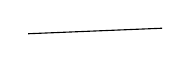
\begin{tikzpicture}
\draw (0,0) -- (1.7,0.07);
\end{tikzpicture}}

J'ai envie de présenter sous une forme légèrement différente la notion de L-groupe\inserted{ $\Pi$,} en termes de la donnée d'un $\mathbb Z$-module $T$ libre de rg $1$ (le $\mathbb Z$-module d'orientations) et d'une \deleted{famille} \inserted{\unsure{ensemble fini}} $(k_i^{\unsure{\natural}})_{i\in I}$ de \uline{germes} \uline{d'hom.} extérieurs
\[
\begin{gathered}
k_i^{\unsure{\natural}}:\quad \deleted{\unsure{\mathbb Z}}\inserted{T}\longrightarrow\Pi
\qquad (i\in I)\\
(\text{\uline{germe} d'hom. ext.})
\end{gathered}
\tag{5}
\]
,

où la notion de ``germe'' est relative à celle des sous-groupes d'indice fini de $T$. \deleted{L'axiome à mettre est} \inserted{\unsure{Pour} une telle donnée,}
\scanpage{189}
\mspage{742}

et tout sous-groupe \deleted{\unsure{à}} $\Pi_0$ de $\Pi$ d'indice fini, on trouve \inserted{pour $\forall i$} un ens de germes d'hom extérieurs
\[
T\longrightarrow\Pi_0
\]
induits par les hom. \deleted{\unsure{ext.}} effectifs $nT\longrightarrow\Pi$ de la classe $k_i^{\unsure{\natural}}$ --- on trouve un nb fini de germes d'hom. ext. $T\longrightarrow\Pi_0$ pour $i$ fixé, de même pour $i$ variable dans $I$. Ceci dit, l'unique axiome d'une L-structure, c'est qu'on puisse trouver un sous-groupe $\Pi_0$ d'indice fini, tel que la ``structure induite'' provienne d'une structure à lacets de $\Pi_0$.

On peut généraliser la notion de L-structure, en s'inspirant de la définition précédente (p. ex), et en y laissant tomber l'exigence que $\Pi_0$ soit d'indice fini --- mais en
\scanpage{190}

prenant soin par contre que $\Pi_0$ soit \uline{distingué}. On exige que \deleted{les} pour $\forall i\in I$, les germes d'hom $k_i:\deleted{\unsure{n}}T\longrightarrow\Pi$ de la classe $k_i^{\unsure{\natural}}$ se factorisent par $\Pi_0$ --- ce qui donne un ens. de \inserted{germes d'}hom extérieurs de $T$ dans $\Pi_0$ ---
\margin{NB il n'est pas clair a priori que cet ens. de germes d'hom. ext. soit fini}
et on exige que cette \deleted{ens. de} \inserted{structure-là} sur $\Pi_0$ provienne \inserted{(pour $\Pi_0$ convenable)} d'une structure à lacets sur $\Pi_0$, \unsure{$\xi$|\&} évidemment uniquement déterminée, une fois $\Pi_0$ choisi. Quant à $\Pi_0$, il est défini à commensurabilité près --- i.e. si $\Pi_0,\Pi'_0$ conviennent, alors $\Pi_0\inserted{\cap}\Pi'_0$ est d'indice fini dans $\Pi_0$ et $\Pi'_0$, et convient également.

\deleted{M'inspirant de la terminologie ``métabélienne'',} j'ai envie (à défaut d'une meilleure suggestion) d'appeler les groupes $\Pi$ munis d'une telle
% ===== LM_C4-191-209: first pass, with mechanical fixes =====
\scanpage{191}
\mspage{743}

structure -- liée à une classe de sous-groupes discrets commensurables entre eux -- \unsure{des|de} \deleted{\unsure{méta-}}\inserted{$L$-$T$-}groupes. (où $L$ est initiale de ``lacets'', et $T$ de ``Teichmüller'') -- ce sont des sortes de \unsure{mixtures} de groupes de Teichmüller et de $L$-groupes. Pour illustrer ce point, partons d'une extension
\diagram{(6)\qquad
\begin{tikzcd}[ampersand replacement=\&, column sep=large]
1 \arrow[r] \& \Pi \arrow[r] \& \mathcal{G} \arrow[r] \& \mathcal{T} \arrow[r] \& 1
\end{tikzcd}
}
où $\Pi$ est muni d'une $L$-structure invariante par $\mathcal{G}$, alors $\mathcal{G}$ est un $L$-$T$-groupe admettant (si $\Pi$ est $\overline{\mathrm m}$ un \deleted{\unsure{$L$-}}groupe à lacets) $\Pi$ comme sous-groupe de définition. Partant du groupe à lacets $\Pi$, on peut prendre p.ex.
\[
(7)\qquad
\left\{
\begin{array}{l}
\mathcal{G}=\mathrm{Aut}_{L}(\Pi)\\
\mathcal{T}=\mathrm{Autext}_{L}(\Pi)
\end{array}
\right.
\qquad\text{d'où}
\,,
\]
\scanpage{192}

et ainsi le groupe \unsure{ambiant} $\mathcal{G}$, extension du groupe de Teichmüller $\mathcal{T}$ par le groupe à lacets $\Pi$, apparaît comme un $LT$-groupe.

\deleted{\unsure{2}}
\scanpage{193}
\mspage{744}

2$^\circ$) \uline{Cas profini}

L'extension de la notion de $L$-groupe ou de $LT$-groupe \inserted{$\Pi$}, en termes de \uline{germes} d'hom extérieurs
\diagram{(8)\qquad
\begin{tikzcd}[ampersand replacement=\&]
\unsure{K_i^{\mathcal{G}}|\kappa_i^{\mathcal{G}}}\colon T \arrow[r] \& \Pi
\end{tikzcd}\,,
}
est essentiellement évidente. Voici l'exemple le plus important pour nous. \deleted{\unsure{Soit}}

Soit d'abord $k$ un corps \deleted{alg. clos de car. $0$}, et soit $M$ une \deleted{\unsure{0-conn.}} \deleted{\unsure{0-connexe}} multiplicité algébrique sur $k$, qui soit \inserted{0-connexe,} de t.f. sur $k$, \deleted{lisse} séparée$/k$ et lisse \unsure{en|de} dim relative $1$. On doit pouvoir \unsure{prouver} alors que $M$ peut se décrire par une courbe alg. lisse et quasi-projective $U$ sur $k$, un groupe fini \deleted{$\unsure{K}$} $G$ qui opère sur $U$, \deleted{et} comme
\[
(9)\qquad M=(U,G)=
\begin{array}{l}
\inserted{\text{(petit)}}\text{ Topos annelé des}\\
\text{faisceaux étales sur}\\
U\text{ où }G\text{ opère}\ldots
\end{array}
\]
\scanpage{194}

\deleted{\unsure{ou}} -- Plus intrinsèquement, il doit être vrai qu'il existe un rev. étale fini de $M$ (qu'on peut supposer galoisien, de groupe $G$) \deleted{\unsure{tel|et}} qui \unsure{soit|est} \unsure{une|un} \deleted{courbe algébrique}\inserted{schéma} -- laquelle \unsure{sera|ser.} néc. \unsure{quasi-projectif|quasi-projective}, lisse, de dim relative $1$ sur $k$. Supposons en tous cas qu'il en soit ainsi, choisissons un pt base géom. $a$ de $M$, et considérons
\[
(10)\qquad \Pi=\Pi_1(M,a)\simeq\Pi_1(\unsure{U|M},G;a)\,.
\]

Nous supposerons désormais $k$ de car. zéro. Supposons d'abord $k$ alg clos. Utilisant la suite exacte
\diagram{(11)\qquad
\begin{tikzcd}[ampersand replacement=\&, column sep=large]
1 \arrow[r] \& \underbrace{\Pi_1(U,a)}_{\Pi_0} \arrow[r] \& \underbrace{\Pi_1(\unsure{U|M},G;a)}_{\Pi} \arrow[r] \& G \arrow[r] \& 1
\end{tikzcd}
}
et la \deleted{\unsure{$L$}} structure à lacets naturelle sur $\Pi_0$, on trouve une $L$-structure sur $\Pi=\Pi_1(\unsure{M},a)$, qui manifestement ne
\scanpage{195}
\mspage{745}

dépend pas du choix du rev. étale \inserted{fini} galoisien $U$ de $M$, et du relèvement choisi du pt géom. $a$ de $M$ en un pt. géom. de $U$. Nous munirons tjrs \inserted{tacitement} $\Pi=\Pi_1(M,a)$ de cette $L$-structure.

Si à nouveau $k$ est un corps \unsure{quelcon-que|quelconque} (le cas le plus intéressant étant celui où $k$ est ext. de type fini de $\mathbb{Q}$), on aura une suite exacte
\diagram{(12)\qquad
\begin{tikzcd}[ampersand replacement=\&, column sep=large]
1 \arrow[r] \& \Pi_1(M_{\overline{k}},a) \arrow[r] \& \Pi_1(M,a) \arrow[r] \& \Gamma_{\overline{k}/k} \arrow[r] \& 1
\end{tikzcd}
}
et $\Pi_1(M_{\overline{k}},\unsure{a|o})$ apparaît comme muni d'une $L$-structure invariante par $\Pi_1(M,\unsure{a|o})=\Pi$, de sorte que $\Pi$ apparaît comme un $TL$-groupe.

Je suis particulièrement intéressé au cas ``universel'' de type $(g,\nu)$ -- mais la base \inserted{naturelle} n'est pas alors le
\scanpage{196}
\mspage{\deleted{\unsure{745}}}

spectre d'un corps $k$, mais la \deleted{\unsure{schéma}} \inserted{multiplicité} modulaire $M_{g,\nu}$. [À vrai dire, pour la structure de $L$-groupe discret $\Pi_0$, jouant le rôle de groupe de référence, on \deleted{peut} \inserted{doit pouvoir} introduire une \deleted{\unsure{schéma}} \inserted{multiplicité} modulaire correspondante sur $\mathbb{Q}$, et $\overline{\mathrm m}$ sur $\mathbb{Z}$. Le fait qui risque de faire des difficultés \unsure{conceptuelles} pour une telle construction, c'est qu'une multiplicité \inserted{``modulaire''} (sur $\mathbb{Q}$, ou sur $\mathbb{Z}$\ldots) décrit en principe une \uline{catégorie} fibrée --- telle celle des schémas en courbes relatifs de type $(g,\nu)$ --- alors que les $\unsure{1|L}$-multiplicités relatives correspondantes à un ``type'' $\Pi_0$-donné forment une \uline{2-catégorie} \inserted{(en groupoïdes)} fibrée sur $(\mathrm{Sch})$, et pas seulement une \uline{catégorie} fibrée\ldots]
\scanpage{197}
\mspage{746}

On aura donc une suite exacte
\diagram{\begin{tikzcd}[ampersand replacement=\&, column sep=small]
(13)\quad 1 \arrow[r] \&
\widehat{\Pi}_{g,\nu} \arrow[r] \&
\underbrace{\Pi_1({\unsure{U|M}_{g,\nu}}_{\mathbb{Q}})}_{\mathcal{M}_{g,\nu}} \arrow[r] \&
\underbrace{\Pi_1({M_{g,\nu}}_{\mathbb{Q}})}_{\mathcal{N}_{g,\nu}} \arrow[r] \& 1,
\end{tikzcd}}
où ${U_{g,\nu}}_{\mathbb{Q}}$ est la courbe \unsure{de|du} type $g,\nu$ universelle'' (en car. $0$). Ici c'est $\Pi_1(U_{g,\nu}\unsure{\deleted{\mathbb{Q}}|\xi}_{\mathbb{Q}})$ qui apparaît comme un $TL$-groupe profini.

Je voudrais dégager une propriété commune à ce cas ``universel'' (13), \deleted{\unsure{et}} \deleted{(qui \unsure{se} \unsure{ramène} d'ailleurs \unsure{essentielle-|essentiellement}} \inserted{et au cas d'une multiplicité} à un corps de base $k$ extension \uline{de type fini} de $\mathbb{Q}$ (le premier cas se ramenant d'ailleurs essentiellement au second, en prenant un ``point générique'' de $M_{g,\nu}$\ldots). Pour ceci, considérons un $LT$-groupe $\unsure{\mathcal{M}|\mathcal{A}}$, et un \deleted{de} homomorphisme
\diagram{\begin{tikzcd}[ampersand replacement=\&]
\unsure{k_i|\kappa_i}:T \arrow[r] \& \deleted{\unsure{\mathcal{G}|\Pi}}\,\mathcal{M}
\end{tikzcd}}
appartenant à un des $\unsure{K_i^{\mathcal{G}}|\kappa_i^{\mathcal{G}}}$. On peut
\scanpage{198}

p. ex. choisir un sous-groupe de définition distingué $\Pi$ dans $\mathcal{M}$, qui sera donc un groupe à lacets, \deleted{\unsure{et on aura|et on a}} une suite exacte
\diagram{\begin{tikzcd}[ampersand replacement=\&, column sep=small]
(14)\quad 1 \arrow[r] \& \Pi \arrow[r] \& \mathcal{M} \arrow[r] \& \mathcal{N} \arrow[r] \& 1,
\end{tikzcd}}
et un \unsure{hom|lacet}
\diagram{(15)\qquad \begin{tikzcd}[ampersand replacement=\&]
\unsure{k|\kappa}:T \arrow[r,hook] \& \Pi
\end{tikzcd},\qquad
$\unsure{k|\kappa}(T)\overset{\mathrm{dfn}}{=}L$
}
relatif à la structure à lacets de $\Pi$. Considérons le normalisateur de $\unsure{L|T}$ dans $\mathcal{M}$
\[
(16)\qquad \operatorname{Norm}_{\mathcal{M}}(L)\overset{\mathrm{dfn}}{=}N(L)
\]
et considérons l'action de $N(L)/L\subset\mathcal{N}$ \deleted{\unsure{dans}} sur $L$. (\uline{NB} On voit aisément que l'image de $N(L)/L$ dans $\mathcal{N}$ est un sous-groupe ouvert de $\mathcal{N}$\ldots) Cette action se fait par un ``\unsure{caractère} cyclotomique'', induit par un \unsure{caractère}
\diagram{(17)\qquad \begin{tikzcd}[ampersand replacement=\&]
\mathcal{N} \arrow[r,"\chi_{\mathcal{N}}"] \& \widehat{\mathbb{Z}}^{*}
\end{tikzcd}.}
L'hypothèse essentielle est que l'image
\scanpage{199}
\mspage{747}

de $\deleted{\chi}\;\mathcal{N}$ par $\chi$ (ou aussi de $N(L)/L$ par $\chi$) soit un sous-groupe ouvert de $\widehat{\mathbb{Z}}^{*}$. Cette hypothèse a un caractère intrinsèque au $LT$-groupe $\mathcal{M}$ lui-$\overline{\mathrm m}$ (indépendamment du choix de $\Pi$) --- car le caractère cyclotomique
\diagram{(18)\qquad \begin{tikzcd}[ampersand replacement=\&]
\chi_{\mathcal{M}}:\mathcal{M} \arrow[r] \& \widehat{\mathbb{Z}}^{*}
\end{tikzcd}}
a un caractère intrinsèque à $\mathcal{M}$, et l'hypothèse signifie que l'image de ce dernier dans $\widehat{\mathbb{Z}}^{*}$ est ouverte.

Revenant à $L$ et $N(L)$, on voit que l'hypothèse \unsure{faite|faîte} implique ceci:
\[
\begin{array}{ll}
(19)&\text{Tout sous-groupe ouvert de }N(L)/L\\
&\text{opère non trivialement sur }L.
\end{array}
\]

On sait, par des arguments \unsure{standarts|standards} que ceci implique que pour tout \unsure{bon|\deleted{bon}} corps $K$ \deleted{de car. $\unsure{0}$} (notamment un corps $\ell$-adique $\mathbb{Q}_{\ell}$),
\scanpage{200}

et tout hom. de $\mathcal{M}$ dans un groupe $G(K)$; où $G$ est un schéma en groupes de t.f. affine sur $K$; \deleted{\unsure{le|u}}
\diagram{(20)\qquad \begin{tikzcd}[ampersand replacement=\&]
u:\mathcal{M} \arrow[r] \& G(K)
\end{tikzcd},}
la restriction de $u$ à $L$ est ``quasi-unipotente'', i.e.
\[
\begin{array}{ll}
(21)&\exists\ \text{sous-groupe ouvert }L'\text{ de }L,\text{ tel que}\\
&u(L')\subset G(K)\text{ soit formé d'éléments}\\
&\text{unipotents},
\end{array}
\]
--- ce qui revient au $\overline{\mathrm m}$, si $\ell_i$ est un générateur de $L=L_i$, qu'on ait
\[
\begin{array}{ll}
(22)&u(\ell_i)\text{ est un élément quasi-}\\
&\text{unipotent de }G(K),\text{ i.e. }\exists\ n\in\mathbb{N}^{*},\\
&\text{tel que }\ell_i^{n}\text{ soit unipotent}.
\end{array}
\]
\scanpage{201}
\mspage{748}

\textcircled{\(3^\circ\)}\quad \uline{Enveloppe schématique d'un} \(T\)\unsure{-}\(L\)-\uline{groupe profini} : \inserted{\unsure{\(a)\)}} \uline{Les hom. admissibles.}

Soient \(\mathcal{M}\) un \(T\)-\(L\)-groupe profini, dont le caractère structural (18)
\diagram{\begin{tikzcd}[ampersand replacement=\&]
\mathcal{M} \arrow[r, "\chi_{\mathcal{M}}"] \& \widehat{\mathbb{Z}}^{*}
\end{tikzcd}}
ait une image ouverte, \(\Pi\) un sous-groupe de définition \unsure{distingué} (c'est donc un \deleted{\unsure{\(L\)-}}groupe \inserted{à lacets} profini\unsure{)|]}, et \(\Pi_0\subset\Pi\) un sous-groupe \uline{discret} de \(\Pi\), qui en soit une ``discrétification'' --- c'est donc un \unsure{groupe} à lacets discret, \unsure{etc.|et} \(\Pi\) s'identifie à son complété profini\ldots

Soit \(G_{\mathbb{Q}}\) un schéma en groupes \inserted{affine de t.f.} sur \(\mathbb{Q}\). Soit \(\mathcal{A}_{\mathbb{Q}}\) l'anneau des adèles de \(\mathbb{Q}\)
\[
(23)\qquad \mathcal{A}_{\mathbb{Q}}=\widehat{\mathbb{Z}}\otimes_{\mathbb{Z}}\mathbb{Q}\subset\prod_{\ell\in\mathbb{P}}\mathbb{Q}_{\ell}
\]
et considérons \unsure{\deleted{le}|le} groupe des points adéliques
\[
(24)\qquad G(\mathcal{A}_{\mathbb{Q}})\subset\prod_{\ell\in\mathbb{P}}G(\mathbb{Q}_{\ell}).
\]
Si \(G_{\mathbb{Q}}\) provient de un \unsure{schém.|schéma} en groupes
\scanpage{202}

affine de t.f. \(G\) sur \(\mathbb{Z}\), alors on a
\[
\begin{gathered}
(25)\qquad G(\mathcal{A}_{\mathbb{Q}})\simeq
\unsure{(|\{}(x_{\ell})_{\ell\in\mathbb{P}}\in\prod_{\ell}G(\mathbb{Q}_{\ell})
\mid x_{\ell}\in G(\mathbb{Z}_{\ell})\\
\hfill\text{pour presque }\unsure{\forall|\mathrm{tt}}\ell\}
\end{gathered}
\]

\deleted{On dit qu'\unsure{un|on}}

On se donne de plus un hom
\diagram{\begin{tikzcd}[ampersand replacement=\&]
(26)\quad G_{\mathbb{Q}} \arrow[r, "\chi_G"] \& \unsure{\mathbb{G}_{m\mathbb{Q}}|G_{m\mathbb{Q}}}.
\end{tikzcd}}
On s'intéresse à \deleted{\unsure{un|ces}}\inserted{des} homomorphismes de groupes
\diagram{\begin{tikzcd}[ampersand replacement=\&]
(27)\quad \mathcal{M} \arrow[r] \& G(\mathcal{A}_{\mathbb{Q}})
\end{tikzcd}}
satisfaisant à des propriétés que nous allons énumérer.

\(1^\circ)\) \uline{Continuité}. Cela équivaut à dire que \(a)\) les hom \(\mathcal{M}\longrightarrow G(\unsure{\mathbb{Q}_{\ell}})\) sont \unsure{continus|continues}, et \(b)\) \(\exists S\) partie finie de \(\mathbb{P}\), telle que pour \(\ell\notin S\), on ait \deleted{\illegible{1}} une factorisation (continue)
\diagram{\begin{tikzcd}[ampersand replacement=\&]
(28)\quad \mathcal{M} \arrow[r] \& G(\widehat{\mathbb{Z}}_{\ell}) \& (\ell\in\mathbb{P}\setminus S)
\end{tikzcd}}
--- condition qui en effet ne dépend pas du ``modèle sur \(\mathbb{Z}\)'' \(G\) de \(G_{\mathbb{Q}}\) choisi.

\uline{NB} (28) est un hom. de groupes profinis.
\scanpage{203}
\mspage{749}

\uline{ReNB} Sauf erreur, la propriété \(1^\circ)\) signifie que l'on peut trouver un schéma en groupes \(G\) affine de t.f. sur \(\mathbb{Z}\), qui \unsure{définisse|définit} \(G_{\mathbb{Q}}\), et tel que (27) se factorise par \(G(\widehat{\mathbb{Z}})\).
\diagram{\begin{tikzcd}[ampersand replacement=\&]
(29)\quad \deleted{\unsure{G}}\quad \mathcal{M} \arrow[r] \& G(\widehat{\mathbb{Z}}).
\end{tikzcd}}

\(2^\circ)\) \uline{Compatibilité avec} \(\chi\) :

\(\unsure{(30)}\)
\diagram{\begin{tikzcd}[ampersand replacement=\&, row sep=large, column sep=large]
\& \mathcal{M} \arrow[r] \arrow[dl, "\chi_{\mathcal{M}}"'] \& G(\mathcal{A}_{\mathbb{Q}}) \arrow[dl, "\chi_G"] \\
\widehat{\mathbb{Z}} \arrow[r, hook] \& \unsure{\mathbb{G}_m|G_m}(\mathcal{A}_{\mathbb{Q}})\simeq\mathcal{A}_{\mathbb{Q}}^{*}\subset\displaystyle\prod_{\ell\in\mathbb{P}}\mathbb{Q}_{\ell}^{*} \&
\end{tikzcd}}
est commutatif.

\(3^\circ)\). \uline{Compatibilité avec la discrétification} \(\Pi_0\).

\((31)\)
\diagram{\begin{tikzcd}[ampersand replacement=\&, row sep=large, column sep=large]
\Pi'_0 \arrow[r, hook] \arrow[d, "\text{factorisation}"] \& \Pi \arrow[r, hook] \& \mathcal{M} \arrow[d] \\
G(\mathbb{Q}) \arrow[rr, hook] \&\& G(\mathcal{A}_{\mathbb{Q}})
\end{tikzcd}},
pour un sous-groupe d'indice fini convenable \(\Pi'_0\) de \(\Pi_0\).

\uline{NB} Quitte à changer de notations \unsure{ops|qps} \(\Pi'_0=\Pi_0\).

\(4^\circ)\) \uline{Caractère minimal} (\unsure{irrédondance|irrédundance}) :

Si \(G'_{\mathbb{Q}}\) est un sous-schéma en groupes de
\scanpage{204}

\(G_{\mathbb{Q}}\), tel que \(\deleted{\unsure{G}}\ \mathcal{M}\longrightarrow G(\mathcal{A}_{\mathbb{Q}})\) se factorise par \(G'(\mathcal{A}_{\mathbb{Q}})\), alors \(G=G'\).

\uline{NB} Si cette hypothèse n'est pas vérifiée, alors parmi tous les \(G'_{\mathbb{Q}}\subset G_{\mathbb{Q}}\) qui la mettent en défaut, il y en a un \inserted{(unique)} plus petit, et en remplaçant \(\chi_G\) par \(\chi_{G'}=\chi_G\mid G'_{\mathbb{Q}}\ldots\), les hyp. \(1^\circ):4^\circ)\) sont satisfaites pour \(G'_{\mathbb{Q}},\chi'\), et \(\mathcal{M}\longrightarrow G'(\mathcal{A}_{\mathbb{Q}})\).

\uline{Remarque}. Soit \(\mathcal{G}_0\subset\mathcal{M}\) le sous-groupe de \(\mathcal{M}\) formé des \(g\in\mathcal{M}\) qui sont tels que \(\unsure{g(\Pi_0)|g\ell(\Pi_0)}\) et \(\Pi_0\) soient commensurables. \unsure{Càd.|C.à.d.} \inserted{les \(g\)} qui normalisent le ``germe de discrétification'' \(\Pi_0\) de \(\Pi\).

\margin{\(\mathcal{G}_0/\unsure{\Pi_0}\) joue le rôle d'un groupe de Teichmüller \uline{discret}}

Il est possible qu'il faille renforcer la condition \(3^\circ\), en exigeant que l'on ait
\diagram{\begin{tikzcd}[ampersand replacement=\&]
\mathcal{G}_0 \arrow[r] \& G(\mathbb{Q}).
\end{tikzcd}}
L'avenir le décidera !
\scanpage{205}
\mspage{750}

Réflexion \unsure{faite|fait}, je préfère poser les choses de façon légèrement \unsure{différente|différent}, en introduisant, dans le \(LT\)-groupe \inserted{profini} \(\mathcal{M}\), un sous-groupe \deleted{\unsure{définissant la \(LT\)-structure|définissant la \(LT\)-struct.}} distingué \(\Pi\) avec une \(L\)-structure (pas \unsure{néc.\textsuperscript{t}|néc.} une structure à lacets --- p.ex. on peut avoir \(\Pi=\mathrm{SL}\unsure{(}2,\mathbb{Z})\)) définissant la \(LT\)-structure de \(\mathcal{M}\), une discrétification \(\Pi_0\) de \(\Pi\) (dans un sens évident, pour les \(L\)-structures) un sous-groupe discret \(\mathcal{G}_0\) \inserted{\(\supset\Pi_0\)} normalisant \(\Pi_0\) (NB. en cas particuliers \unsure{importants} on \(\mathcal{G}_0=\Pi_0\)), tel que \inserted{son adh.} \(\unsure{\widehat{\mathcal{G}}_0|\mathcal{G}_0^{*}}\) \inserted{\(\overset{\mathrm{dfn}}{=}\mathcal{G}\)} dans \(\mathcal{M}\) soit distingué dans \(\mathcal{M}\).

On a donc un diagramme de groupes

\((32)\)
\diagram{\begin{tikzcd}[ampersand replacement=\&, 
row sep=large, column sep=large,
execute at end picture={
  \path (s205p.north) -- coordinate[midway] (s205pgmid) (s205g.north);
  \path (s205g.north) -- coordinate[midway] (s205gmmid) (s205m.north);
  \path (s205p.north) -- coordinate[midway] (s205pmmid) (s205m.north);
  \path (s205pzero.south) -- coordinate[midway] (s205zeromid) (s205gzero.south);
  \draw ([yshift=5mm]s205p.north) .. controls ([yshift=8mm]s205p.north) and ([xshift=-2mm,yshift=5mm]s205pgmid) .. ([yshift=8mm]s205pgmid) .. controls ([xshift=2mm,yshift=5mm]s205pgmid) and ([yshift=8mm]s205g.north) .. ([yshift=5mm]s205g.north);
  \node[above] at ([yshift=8mm]s205pgmid) {$\mathcal{T}$};
  \draw ([yshift=5mm]s205g.north) .. controls ([yshift=8mm]s205g.north) and ([xshift=-2mm,yshift=5mm]s205gmmid) .. ([yshift=8mm]s205gmmid) .. controls ([xshift=2mm,yshift=5mm]s205gmmid) and ([yshift=8mm]s205m.north) .. ([yshift=5mm]s205m.north);
  \node[above] at ([yshift=8mm]s205gmmid) {$\Gamma$};
  \draw ([yshift=17mm]s205p.north) .. controls ([yshift=20mm]s205p.north) and ([xshift=-2mm,yshift=17mm]s205pmmid) .. ([yshift=20mm]s205pmmid) .. controls ([xshift=2mm,yshift=17mm]s205pmmid) and ([yshift=20mm]s205m.north) .. ([yshift=17mm]s205m.north);
  \node[above] at ([yshift=20mm]s205pmmid) {$\mathcal{N}$};
  \draw ([yshift=-3mm]s205pzero.south) .. controls ([yshift=-6mm]s205pzero.south) and ([xshift=-2mm,yshift=-3mm]s205zeromid) .. ([yshift=-6mm]s205zeromid) .. controls ([xshift=2mm,yshift=-3mm]s205zeromid) and ([yshift=-6mm]s205gzero.south) .. ([yshift=-3mm]s205gzero.south);
  \node[below] at ([yshift=-6mm]s205zeromid) {$\mathcal{T}_0$};
}]
\unsure{1} \arrow[r, hook] \& |[alias=s205p]| \underset{=\widehat{\Pi}_0}{\Pi} \arrow[r, hook] \& |[alias=s205g]| \underset{=\widehat{\mathcal{G}}_0}{\unsure{\widehat{\mathcal{G}}|\mathcal{G}^{*}}_{\unsure{\deleted{0}|0}}} \arrow[r, hook] \& |[alias=s205m]| \mathcal{M} \\
1 \arrow[r, hook] \& |[alias=s205pzero]| \Pi_0 \arrow[u, hook] \arrow[r, hook] \& |[alias=s205gzero]| \mathcal{G}_0 \arrow[u, hook] \&
\end{tikzcd}},

où la première ligne est formée de groupes profinis, la deuxième de groupes discrets. On notera que \(\mathcal{G}\) s'identifie à un quotient du complété profini de \(\mathcal{G}_0\), mais
\scanpage{206}

je n'exige pas pour le moment qu'il soit isomorphe à ce complété lui-$\overline{\mathrm m}$. \unsure{Donc} \unsure{idem|item} pour $\mathcal{T}$ et $\mathcal{T}_0$. Le groupe $\mathcal{T}_0\inserted{=\mathcal{G}_0/\Pi_0}$ joue le rôle d'un groupe de Teichmüller \inserted{``absolu''} discret, le groupe $\mathcal{T}$ celui d'un complété de gr. de Teichmüller, le groupe $\Gamma=\mathcal{M}/\mathcal{G}$ joue le rôle d'un groupe de Galois profini. \deleted{La \unsure{situation}} Je suis intéressé surtout par deux situations extrêmes

a) $\mathcal{G}_0=\Pi_0$ d'où $\mathcal{G}=\Pi$ --- situation provenant d'une \unsure{$1$-multiplicité} lisse relative sur un corps \deleted{$k$} ext. de t.f. de $\mathbb{Q}$, ou plus généralement \deleted{d'un schéma}\inserted{sur un} schéma \inserted{(ou une multiplicité)} \unsure{int.} de type fini sur $\mathbb{Q}$, \deleted{\unsure{$\Gamma$|$k$} \unsure{en fait}}\inserted{$\mathcal{N}\unsure{\xrightarrow{\sim}|\simeq}\Gamma$, est} \deleted{\unsure{est}} le groupe fondamental \deleted{de cette} schéma ou de la dite multiplicité,

b) $\mathcal{G}_0/\Pi_0\simeq$ groupe de Teichmüller de $\Pi_0$ \inserted{ou d'indice fini dans ce gr. de T.} --- dans ce cas, on est intéressé surtout à une situation ``modulaire'', où
\scanpage{207}
\mspage{751}

$\mathcal{N}$ s'interprète comme le groupe fondamental de \unsure{la|leur} multiplicité modulaire universelle, $\mathcal{T}$ comme sa partie ``géométrique'', $\mathcal{T}_0$ comme sa partie ``transcendante'', et $\Gamma$ comme $\Gamma_{\unsure{\overline{\mathbb{Q}}_0|\overline{\mathbb{Q}}}/\mathbb{Q}}$ ....

On fait sur (32) l'hypothèse que le caractère cyclotomique sur $\mathcal{M}$ (opérant sur $\Pi$ par autom. de $L$-structures) soit trivial sur $\mathcal{G}$, a fortiori sur $\Pi$ (donc
\[
(33)\qquad \Pi=\Pi^{+},\quad \mathcal{G}=\mathcal{G}^{+}\qquad ),
\]
i.e. qu'il se factorise en
\diagram{(34)\qquad
\begin{tikzcd}[ampersand replacement=\&, column sep=large]
\Gamma \arrow[r, "\chi_{\Gamma}"] \& \widehat{\mathbb{Z}}^{*}
\end{tikzcd},
}
\uline{dont l'image est un ss-groupe ouvert.}

Si $(G_{\mathbb{Q}},\chi_G)$ est comme plus haut (p. 748), on s'intéresse aux hom (27)
\diagram{
\begin{tikzcd}[ampersand replacement=\&, column sep=large]
\mathcal{M} \arrow[r] \& G(\mathcal{A}_{\mathbb{Q}})
\end{tikzcd}
}
satisfaisant les conditions $1^{\circ})$ $2^{\circ})$ $\deleted{\unsure{2}}\inserted{3}^{\circ})$ $4^{\circ})$ comme dessus, mais où $3^{\circ})$ est \unsure{formulée} sous la forme un peu plus forte

($3^{\circ}$ forte) (Compatibilité avec discrétification de Teichmüller $\mathcal{G}_0$) : On a une \unsure{factorisa-}
\scanpage{208}

tion $\mathcal{G}_0\longrightarrow G(\mathbb{Q})$, rendant \unsure{donc} commutatif le diagramme
\diagram{(35)\qquad
\begin{tikzcd}[ampersand replacement=\&, column sep=large, row sep=large]
\mathcal{G}_0 \arrow[r, hook] \arrow[d] \& \mathcal{M} \arrow[d] \\
G(\mathbb{Q}) \arrow[r, hook] \& G(\mathcal{A}_{\mathbb{Q}})
\end{tikzcd}.
}

Les structures de la forme (32) méritent sans doute un nom, je vais \unsure{les} appeler --- ne serait-ce que provisoirement, \uline{\unsure{structures} de Galois-Teichmüller.}
\margin{Quitte par la suite à introduire des conditions plus draconiennes sur \unsure{cette structure}}

Si $G$ est un groupe algébrique affine sur $\mathbb{Q}$, un hom $\mathcal{M}\unsure{\longrightarrow|{-}}G(\mathcal{A}_{\mathbb{Q}})$ satisfaisant les conditions $1^{\circ})$ $2^{\circ})$ $3^{\circ})$ \inserted{(forte)} $4^{\circ})$ est appelé un ``hom de Lie'' de la structure de Galois-Teichmüller.

Je vais désigner par la suite par $\underline{\mathcal{M}}_{\mathbb{Q}}$ \inserted{(ou \unsure{simplement} $\underline{\mathcal{M}}$ ?)} le schéma en groupes \inserted{$G_{\mathbb{Q}}$} sur $\mathbb{Q}$. \deleted{\unsure{défini}}

Je désigne par \deleted{$\unsure{\mathcal{G}|\mathcal{M}}$} $\underline{\mathcal{G}}_{\mathbb{Q}}$ le sous-schéma en groupes de $\underline{\mathcal{M}}_{\mathbb{Q}}$ engendré par l'
\scanpage{209}
\mspage{752}

image de $\mathcal{G}_0\longrightarrow\deleted{\unsure{\mathcal{M}|G}}G(\mathbb{Q})$, par $\underline{\Pi}_{\mathbb{Q}}$ celui engendré par l'image de $\Pi\longrightarrow G(\mathbb{Q})$

On a ainsi \deleted{\unsure{un}} des sous-schémas en groupes
\[
(36)\qquad \underline{\Pi}_{\mathbb{Q}}\subset
\deleted{\underline{\unsure{\mathcal{M}}}}\inserted{\underline{\mathcal{G}}}_{\mathbb{Q}}
\subset\underline{\mathcal{M}}_{\mathbb{Q}}
\]
\uline{distingués} dans $\underline{\mathcal{M}}_{\mathbb{Q}}$, donnant lieu à des schémas en groupes quotients
\[
(37)\qquad
\left\{
\begin{aligned}
&\underline{\mathcal{T}}_{\mathbb{Q}}\simeq
\underline{\mathcal{G}}_{\mathbb{Q}}/\underline{\Pi}_{\mathbb{Q}},\quad
\underline{\Gamma}_{\mathbb{Q}}\simeq
\underline{\mathcal{M}}_{\mathbb{Q}}/\underline{\mathcal{G}}_{\mathbb{Q}},\\
&\qquad\underline{\mathcal{N}}_{\mathbb{Q}}\simeq
\underline{\mathcal{M}}_{\mathbb{Q}}/\underline{\Pi}_{\mathbb{Q}}
\end{aligned}
\right.
\]
--- donnant lieu à quatre suites exactes de schémas en groupes, dont la dernière est
\diagram{(38)\qquad
\begin{tikzcd}[ampersand replacement=\&, column sep=large]
1 \arrow[r] \& \underline{\mathcal{T}}_{\mathbb{Q}} \arrow[r] \&
\underline{\mathcal{N}}_{\mathbb{Q}} \arrow[r] \& \underline{\Gamma}_{\mathbb{Q}} \arrow[r] \& 1
\end{tikzcd}.
}

\deleted{Je \unsure{vais|vois} \unsure{réfléchir|rappeler}}\inserted{Notons \unsure{que}} le caractère $\chi_G:G_{\mathbb{Q}}\longrightarrow \unsure{\mathbb{G}_m|G_m}$ est épi, et se factorise par $\underline{\Gamma}_{\mathbb{Q}}$ en
\diagram{(39)\qquad
\begin{tikzcd}[ampersand replacement=\&, column sep=large]
\underline{\Gamma}_{\mathbb{Q}} \arrow[r, "\chi_{\underline{\Gamma}}"] \& \unsure{\mathbb{G}_{m\mathbb{Q}}|G_{m\mathbb{Q}}}
\end{tikzcd}.
}
% ===== LM_C4-210-228: first pass only (not yet checked) =====
\scanpage{210}
Le système de groupes \inserted{sur $\mathbb{Q}$} (36, 37), muni
de l'hom de
\[
\Pi \subset \mathcal{G} \subset M
\]
dans \deleted{\unsure{$\mathcal{G}$}}
\[
(40)\qquad
\underline{\Pi}_{\mathbb{Q}}(\unsure{\mathbb{A}'_{\mathbb{Q}}})
\subset \underline{\mathcal{G}}_{\mathbb{Q}}(\mathbb{A}_{\mathbb{Q}})
\subset \underline{M}_{\mathbb{Q}}(\unsure{\mathbb{A}_{\mathbb{Q}}})
\]
\deleted{déduit} \inserted{induit} par
$M\longrightarrow \unsure{G}(\mathbb{A}_{\mathbb{Q}})$ (satisfaisant
aux conditions $1^\circ)$ à $4^\circ)$ ci-dessus \deleted{\unsure{)}}, i.e.
d'un ``hom de Lie'') s'appellera aussi
une ``\uline{approximation de Lie}'' du
système de Galois-Teichmüller envisagé.

Considérons un \deleted{germe d'}hom
\[
(41)\qquad k_i^{\deleted{\unsure{\sharp}}}\quad T_0\longrightarrow\Pi_0
\]
\unsure{appartenant|correspondant} à la L-structure de $\Pi$,
définit donc \inserted{par composition avec
$\unsure{\Pi_0}\longrightarrow
\deleted{\unsure{\mathcal{G}}}\underline{\Pi}_{\deleted{\unsure{\mathbb{Q}}}}(\mathbb{Q})$}
un \deleted{germe d'}homomorphisme
\[
(42)\qquad T_0\longrightarrow
\deleted{\unsure{\mathcal{G}}}\underline{\Pi}(\mathbb{Q}).
\]
\margin{\uline{NB} pour $i$ fixé,
$k_i$ est déterminé mod
\unsure{autom.} int. de $\Pi_0$ \uuline{et}
mod composition avec
$n\,\mathrm{id}_{T_0}$, pour $n\in\mathbb{N}^{*}$.
Pour ce qui est de ce dernier point, \unsure{il y a}
\unsure{souvent} (\unsure{fixons} $\Pi_0$) un
``meilleur choix'', dont tous \unsure{les autres se}
déduisent par composition avec
$n\,\mathrm{id}_{T_0}$.}
On voit \inserted{((21) p.\,$747'$)} que cet \deleted{germe de} homomorphisme
est quasi-unipotent, et qu'il définit par
suite un hom de \deleted{\unsure{g}} schémas en groupes
\margin{209}
\scanpage{211}
\mspage{753}
\[
(43)\qquad \underline{k}_i:
\underset{(\simeq G_{a\mathbb{Q}}\otimes_{\mathbb{Z}}T_0)}{\underline{T}_{0\mathbb{Q}}}
\longrightarrow \underline{\Pi}_{\mathbb{Q}}
\]
(pas seulement un germe!)
qui définit, par \deleted{composition} passage aux
pts $\mathbb{Q}$-rationnels, le \uline{germe} d'hom
(42). On trouve ainsi un ens. fini
(indexé par \inserted{l'ens} des germes de \uline{sous-groupes}
lacets de $\Pi_0$, ou de $\Pi$ ce qui revient \unsure{au}
$\unsure{\overline{\mathrm m}}$) des hom extérieurs (43) de schémas
en groupes. J'ai envie d'appeler l'appro-\deleted{\unsure{représentation}}\inserted{ximation} de Lie \uline{non dégénérée} si
les hom précédents sont tous non
triviaux, donc sont des \uline{mono.}
\[
(44)\qquad \underline{k}_i:
\underline{T}_{0\mathbb{Q}}\simeq G_{a\mathbb{Q}}\otimes_{\mathbb{Z}}T_0
\lhook\joinrel\longrightarrow \underline{\Pi}_{\mathbb{Q}}.
\]

Supposons que $\underline{M}_{\mathbb{Q}}$ provienne
d'un schéma en groupes (affine \unsure{et} t.f.)
$\underline{M}$ sur $\mathbb{Z}$, tel que l'on ait
\[
(45)\qquad M\longrightarrow\underline{M}(\widehat{\mathbb{Z}})
\]
(il me semble qu'on peut tjrs trouver un
tel $\underline{M}$...). On désigne alors par
\margin{210}
\scanpage{212}
$\underline{\Pi}$, $\underline{\mathcal{G}}$ les adhérences schématiques dans
$\underline{M}$ de $\underline{\Pi}_{\mathbb{Q}}$, $\underline{\mathcal{G}}_{\mathbb{Q}}$, d'où un diagramme
de schémas en groupes sur $\mathbb{Z}$
\[
(46)\qquad
\diagram{\begin{tikzcd}[ampersand replacement=\&,column sep=3em]
\underline{\Pi}
\arrow[r,phantom,"\subset" description]
\arrow[r,no head,to path={(\tikztostart.north) -- ++(0,0.35) -| (\tikztotarget.north) \tikztonodes},"\underline{\unsure{\mathcal{T}}}"]
\arrow[rr,no head,to path={(\tikztostart.south) -- ++(0,-0.35) -| (\tikztotarget.south) \tikztonodes},"\underline{N}"']
\&\underline{\mathcal{G}}
\arrow[r,phantom,"\subset" description]
\arrow[r,no head,to path={(\tikztostart.north) -- ++(0,0.35) -| (\tikztotarget.north) \tikztonodes},"\underline{\Gamma}"]
\&\underline{M}
\end{tikzcd}}
\]
(sous réserve de représentabilité des
quotients $\underline{\unsure{\mathcal{T}}}$, $\underline{\Gamma}$, $\underline{N}$ --- mais je crois que
pour Raynaud il n'y a jamais de pb...).
On \deleted{\unsure{va supposer|suppose} bien sûr que}
\inserted{aura des factorisations}
\[
(47)\qquad
\diagram{\begin{tikzcd}[ampersand replacement=\&,column sep=large,row sep=large]
\Pi_0\arrow[r,hook,no head]\arrow[d]
\&\mathcal{G}_0\arrow[r,hook]\arrow[d]
\&M\arrow[d]\\
\underline{\Pi}(\mathbb{Z})\arrow[r,hook]
\&\underline{\mathcal{G}}(\mathbb{Z})\arrow[r,hook,no head]
\&\underline{M}(\widehat{\mathbb{Z}}).
\end{tikzcd}}
\]

On suppose bien sûr \deleted{\unsure{(y a-t-il}} que
l'hom $\chi_{\underline{\unsure{M}}}:\deleted{\unsure{\mathbb{Q}}}\underline{M}_{\mathbb{Q}}\longrightarrow G_{m\mathbb{Q}}$ se
prolonge en
\[
(48)\qquad \chi_{\underline{M}}:\underline{M}\longrightarrow G_{m\mathbb{Z}},
\]
lequel évidemment se factorise par
\[
(49)\qquad \chi_{\underline{\Gamma}}:\underline{\Gamma}\longrightarrow G_{m\mathbb{Z}}.
\]
\margin{211}
\scanpage{213}
\mspage{754}
Il serait intéressant de dégager un th. d'existence,
(voir \inserted{\unsure{même}} d'unicité, moyennant des conditions plus fortes
encore) d'un ``modèle'' $\underline{M}$ \inserted{\uline{lisse}} sur $\mathbb{Z}$ de $\underline{M}_{\mathbb{Q}}$,
satisfaisant aux conditions précédentes
\figure{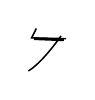
\begin{tikzpicture}[x=0.5cm,y=0.5cm,baseline=0]
\draw[line width=0.55pt] (0.12,0.72)--(0,0.48)--(0.88,0.46);
\draw[line width=1pt] (0.06,0.46)--(0.82,0.43);
\draw[line width=0.55pt] (0.75,0.53) .. controls (0.48,0.16) and (0.18,-0.2) .. (-0.08,-0.36);
\end{tikzpicture}}
\[
(M\longrightarrow\underline{M}(\mathbb{Z}),\quad
\text{et }\underline{M}\xrightarrow{\chi_{\underline{M}}}G_{m\mathbb{Z}}).
\]

Ici il ne sera plus vrai en général, je
présume, que les hom. extérieurs \inserted{$\underline{k}_i$} (43) se
prolongent tels quels en des hom
$\underline{T}_i\underset{\deleted{\unsure{\to}}}{=}\underline{T}_{i\mathbb{Z}}\longrightarrow\underline{\Pi}$.
Mais je \unsure{vais|fais} considérer
le centralisateur de $k_i:T_0\longrightarrow\Pi_0$ dans $\Pi_0$,
soit $\widetilde{L}_{i,0}$ qui est un groupe
métabélien : $\operatorname{Im}(T_0\xrightarrow{k_i}\Pi_0)$ y est un
sous-groupe \inserted{distingué} d'indice fini. Considérons
l'hom
\[
(50)\qquad
\diagram{\begin{tikzcd}[ampersand replacement=\&,column sep=large,row sep=small]
\widetilde{L}_{i,0}\arrow[r]\arrow[d,equal]
\&\underline{\Pi}(\mathbb{Z}),\\
\operatorname{Centr}_{\Pi_0}(k_i:T_0\longrightarrow\Pi_0)\&
\end{tikzcd}}
\]
qui est \unsure{ent.} unipotent --- il se factorise
donc par un hom. de schémas en groupes
\[
(51)\qquad \operatorname{Env}(\widetilde{L}_{i,0})\longrightarrow\underline{\Pi}
\]
(cf.\ \S\,50, $4^\circ$, p.\,$658'$ ff), se factorisant
\margin{212}
\scanpage{214}
par un des \inserted{schémas en} groupes lisses \unsure{quotient|quotients} \inserted{$\underline{Z}_{i,n}$} de
$\operatorname{Env}(\widetilde{L}_{i,0})$, dont celui-ci est la $\varprojlim$ :
\[
(52)\qquad
\diagram{\begin{tikzcd}[ampersand replacement=\&,column sep=large,row sep=small]
1\arrow[r,no head]\&\underline{nT_0}\arrow[r]
\&\underline{Z}_{i,n}\arrow[r]
\&(H_{i,n})_{S_0}\arrow[r,no head]\arrow[d,phantom,"\simeq"{description,rotate=90}]
\&1\\
\&\&\& (\widetilde{L}_{i,0}/nT_0)\&
\end{tikzcd}}
\]
\margin{$S_0=\operatorname{Spec}\mathbb{Z}$}
Mais bien entendu, la restriction de l'hom
obtenu
\[
\unsure{(5|(s}\qquad \underline{Z}_{i,n}\longrightarrow\underline{\Pi}
\]
à
\[
\underline{Z}_{i,n}^{\circ}\simeq\underline{nT_0}
\]
n'est pas en général un mono --- s'il
l'est pour $n$ fixé, alors si $n\mid n'$, $n\ne n'$,
il ne l'est plus pour $n'$. Un cas parti-
culièrement favorable serait celui où
on peut trouver $n$ tel que l'hom
induit
\[
(53)\qquad\underline{nT_0}\longrightarrow\underline{\Pi}
\]
\margin{cet $n$ est alors \uline{unique}.}
soit un mono. Cela implique que l'adhérence
schématique dans $\underline{\Pi}$ du ``sous-groupe
additif à $1$ paramètre''
$\deleted{\unsure{\mathcal{G}}}\underline{L}_{i\mathbb{Q}}
=\underline{k}_i(\underline{\unsure{T_0}})$
est un sous-schéma en groupes \uline{lisse} de $\underline{\Pi}$.
\margin{213}
\scanpage{215}
\mspage{755}

Cette condition doit être aussi suffisante -- du moins si on exige que cette adh. schématique ait une comp. neutre qui soit $\unsure{=|\simeq}$ isom. à $\mathrm{G}_{aS_0}$.
On trouve alors, \inserted{en tout cas,} un \uline{monomorphisme} unique (à conjugaison près)
\[
(54)\qquad \deleted{\unsure{k}}\uuline{k_i'}:\quad
\diagram{\begin{tikzcd}[ampersand replacement=\&,column sep=large]
\underline{T_0} \arrow[r,hook] \& \underline{\Pi}
\end{tikzcd}}
\]
tel que $\uuline{k_i'}_{\mathbb{Q}}$ soit de la forme $\underline{k_i}_{\mathbb{Q}}\circ(\unsure{r_i}\mathrm{id})$,
\deleted{pour}\inserted{avec} $\unsure{\parallel|!!}\ \unsure{r_i}\in\mathbb{Q}^{*+}$ convenable.
Je ne suis pas sûr que sous ces conditions, \deleted{on \unsure{puisse} trouver un} \inserted{l'}hom déduit de $\underline{k_i'}$ en passant aux $\mathbb{Z}$-pts
\[
\diagram{\begin{tikzcd}[ampersand replacement=\&,column sep=large]
T_0\simeq\underline{T_0}(\mathbb{Z}) \arrow[r] \& \underline{\Pi}(\mathbb{Z})
\end{tikzcd}}
\]
se factorise en un hom
\[
(55)\qquad
\diagram{\begin{tikzcd}[ampersand replacement=\&,column sep=large]
T_0 \arrow[r,"{k_i'\unsure{\varphi|?}}"] \& \Pi_0 \arrow[r,"{\mathrm{can}}"] \& \underline{\Pi}(\mathbb{Z})
\end{tikzcd}},
\]
\unsure{où} $T_0\longrightarrow\Pi_0$ \unsure{appartienne} au \uline{``germe''} $\underline{k_i}$, $\leftarrow$

Je vais néanmoins le poser comme hypothèse \inserted{suppl.}, lorsque les $\underline{k_i'}$ existent.

J'ai envie d'énoncer quelques autres ``bonnes hypothèses'', qu'on s'efforcera de \unsure{réaliser}
\margin{214}
\scanpage{216}

en travaillant sur des approximations de Lie ``entières'' i.e. sur $\operatorname{Spec}\mathbb{Z}$.

Considérons tous les hom $\underline{k_i'}$ possibles ($i$ variable, mais aussi en conjuguant les $k_i:\deleted{\unsure{T_0}}\ T_0\longrightarrow\Pi_0$ de départ par des éléments quelconques de $\Pi_0$), et les hom correspondants sur les algèbres de Lie
\[
(56)\qquad \operatorname{Lie}(\underline{k_i'}):\quad
\diagram{\begin{tikzcd}[ampersand replacement=\&,column sep=large,row sep=small]
\deleted{\unsure{\mathbb{Z}}}\ T_0 \arrow[r] \arrow[d,phantom,"{\wr}" description] \& \Gamma\underline{\operatorname{Lie}}(\underline{\Pi})\underset{\unsure{\mathrm{df}}}{=}\operatorname{Lie}(\underline{\Pi}) \\
\begin{gathered}\mathbb{Z}\\\text{(pas canonique)}\end{gathered} \&
\end{tikzcd}}
\]
qui est par hyp. un \deleted{\unsure{bon}} \unsure{monomorphisme} \unsure{universel}, on voudrait que $\Gamma\underline{\operatorname{Lie}}(\underline{\Pi})$ soit \uline{engendré} (en tant que $\mathbb{Z}$-module) par leurs images, ou (\unsure{ce} qui revient au $\overline{\mathrm m}$) par les images d'un générateur de $T_0$.
\margin{cette hyp. \unsure{semble} raisonnable dans un cas comme $\Pi_0=\operatorname{SL}(2,\mathbb{Z})$, mais \unsure{non si} $I=\varnothing$ p.ex\ldots !}
\unsure{Il} revient au $\overline{\mathrm m}$ de dire que si on choisit pour $\forall i$ \uline{un} $\underline{k_i'}$, d'où l'image \inserted{dans $\Gamma\underline{\operatorname{Lie}}(\underline{\Pi})$} d'un élt générateur de $T_0$, les $I$ éléments obtenus dans $\deleted{\unsure{\Gamma}}\operatorname{Lie}(\underline{\Pi})$, \uline{et} leurs conjugués par les éléments de $\Pi_0$, engendrent le $\mathbb{Z}$-module $\operatorname{Lie}(\underline{\Pi})$. Ceci \deleted{signifie} implique que
\margin{215}
\scanpage{217}
\mspage{756}

\unsure{ce|le} schéma en groupes $\underline{\Pi}^{\circ}$ sur $S_0=\operatorname{Spec}\mathbb{Z}$, en tant que faisceau étale sur le ``gros topos étale'' de $S_0$, est engendré par \deleted{les}\inserted{un nb fini de} sous-groupes $k_i'(\underline{\mathrm{G}_a})$,
\deleted{et par le groupe discret $\Pi_0$.}
\inserted{(avec répétition possible d'une $\overline{\mathrm m}$ classe de conjugaison), ou encore \deleted{\unsure{plutôt}}\inserted{que} $\underline{\Pi}$ est}
\deleted{(Et il \unsure{se pose} \unsure{infiniment|l'intéressante} \unsure{questi-}}
\inserted{engendré par \unsure{les}}
les $k_i'(\mathrm{G}_a)$ (\unsure{leurs divers conjugués|un de chaque} disons) et le groupe discret $(\Pi_0)_{S_0}$.
(Et il se pose la question intéressante d'expliciter les relations\ldots{} suffit-il d'écrire les relations de $\Pi_0$, plus \unsure{la commutativité} de
\[
(57)\qquad
\diagram{\begin{tikzcd}[ampersand replacement=\&,column sep=large,row sep=large]
T_0 \arrow[r,no head,"{k_i'}"] \arrow[d,"{\mathrm{can}}"] \& \Pi_0 \arrow[d,"{\mathrm{can}}"] \\
\underline{T_0} \arrow[r,"{\underline{k_i'}}"] \& \underline{\Pi}
\end{tikzcd}}
\qquad ?\quad\Big)
\]

Autres conditions, concernant les sch. en groupes
\[
(58)\qquad
\underline{\gamma}_{\underline{\Pi}}=\underline{\Pi}/\underline{\Pi}^{\circ},\quad
\underline{\gamma}_{\underline{\mathcal{G}}}=\underline{\mathcal{G}}/\underline{\mathcal{G}}^{\circ},\quad
\underline{\gamma}_{\underline{M}}=\underline{M}/\underline{M}^{\circ}
\]
-- on voudrait que ce soient des schémas en groupes \uline{constants}, \unsure{correspondant} aux \deleted{\unsure{schémas}} groupes finis discrets qui décrivent les quotients correspondants des groupes sur $\mathbb{Q}$, lesquels groupes discrets sont des quotients
\margin{216}
\scanpage{218}

\[
(59)\qquad
\left\{\begin{array}{l}
\gamma_{\Pi}\ (\text{resp. }\gamma_{\mathcal{G}},\ \text{resp. }\gamma_M)\quad\text{quotients de }\Pi,\mathcal{G},M\\
\underline{\gamma}_{\underline{\Pi}}\simeq(\gamma_{\Pi})_{S_0},\quad
\underline{\gamma}_{\underline{\mathcal{G}}}\simeq(\gamma_{\mathcal{G}})_{S_0},\quad
\underline{\gamma}_{\underline{M}}\simeq(\gamma_M)_{S_0}
\end{array}\right.
\]
qui s'insèrent dans une suite \deleted{exacte}\inserted{d'homs}
\[
(60)\qquad
\diagram{\begin{tikzcd}[ampersand replacement=\&,column sep=large]
\gamma_{\Pi} \arrow[r] \& \gamma_{\mathcal{G}} \arrow[r] \& \gamma_M
\end{tikzcd}}
\]
et dans des suites exactes
\[
(61)\qquad
\left\{\diagram{\begin{tikzcd}[ampersand replacement=\&,column sep=large,row sep=small]
\gamma_{\Pi} \arrow[r,no head] \& \gamma_{\mathcal{G}} \arrow[r] \& \gamma_{\unsure{\mathcal{T}}} \arrow[r] \& 1\\
\gamma_{\Pi} \arrow[r] \& \gamma_M \arrow[r] \& \gamma_N \arrow[r] \& 1\\
\gamma_{\mathcal{G}} \arrow[r] \& \gamma_M \arrow[r,no head] \& \gamma_{\deleted{\unsure{\mathcal{T}}}\Gamma} \arrow[r] \& 1\\
\gamma_{\unsure{\mathcal{T}}} \arrow[r,no head] \& \gamma_N \arrow[r] \& \gamma_{\Gamma} \arrow[r] \& 1
\end{tikzcd}}\right.\quad .
\]

Cette hypothèse sur $\underline{\Pi},\underline{\mathcal{G}},\underline{M}$ permet de définir des groupes $\underline{\Pi}^{\Delta}(\widehat{\mathbb{Z}})^{\unsure{\Delta}},\underline{\mathcal{G}}^{\Delta}(\widehat{\mathbb{Z}})^{\unsure{\Delta}},\underline{M}^{\Delta}(\widehat{\mathbb{Z}})$, et on aura nécessairement les deux premières factorisations de
\[
(62)\qquad
\left\{\diagram{\begin{tikzcd}[ampersand replacement=\&,column sep=large,row sep=large]
\Pi \arrow[r] \& \underline{\Pi}^{\Delta}(\deleted{\unsure{\widehat{\mathbb{Q}}}}\widehat{\mathbb{Z}})\\
\mathcal{G} \arrow[r] \& \unsure{\underline{\mathcal{G}}}^{\Delta}(\widehat{\mathbb{Z}})\\
M \arrow[r] \& \underline{M}^{\Delta}(\widehat{\mathbb{Z}})
\end{tikzcd}}\right.
\]
(car
\[
\diagram{\begin{tikzcd}[ampersand replacement=\&,column sep=large,row sep=small]
\Pi_0 \arrow[r,no head] \& \underline{\Pi}(\mathbb{Z})\subset\underline{\Pi}^{\Delta}(\widehat{\mathbb{Z}})\\
\mathcal{G}_0 \arrow[r,no head] \& \underline{\mathcal{G}}(\mathbb{Z})\subset\underline{\mathcal{G}}^{\Delta}(\widehat{\mathbb{Z}})
\end{tikzcd}}
\qquad).
\]
Quant à la troisième factorisation, elle devrait être incluse dans les conditions de départ d'un hom de Lie d'une structure de Teichmüller - Galois - savoir que $\underline{\unsure{M}}_{\mathbb{Q}}/\underline{\unsure{M}}_{\mathbb{Q}}^{\circ}$ est constant, ce qui permet
\margin{\deleted{\unsure{lisse}}}
\margin{217}
\scanpage{219}
\mspage{757}

alors de définir $\underline{\unsure{M}}_{\mathbb{Q}}^{\Delta}(\unsure{A|\mathbb{A}}_{\mathbb{Q}})$, et on exige que $M\relbar\underline{M}_{\mathbb{Q}}(\unsure{A|\mathbb{A}}_{\mathbb{Q}})$ se factorise par
\[
(63)\qquad
\diagram{\begin{tikzcd}[ampersand replacement=\&,column sep=large]
M \arrow[r,phantom,"{\unsure{\longrightarrow|\Longrightarrow}}" description] \& \underline{M}_{\mathbb{Q}}^{\Delta}(\unsure{A|\mathbb{A}}_{\mathbb{Q}})
\end{tikzcd}}\quad .
\]

Si de plus on suppose que les \unsure{images} des trois hom (62) sont des \unsure{sous-groupes} \uline{ouverts}, (condition qui renforce considérablement la condition d'\unsure{indice} \unsure{donnée} $4^\circ$) (p. 749), pourvu qu'on la conjugue avec la surjectivité des composés
\[
(64)\qquad
\left\{\diagram{\begin{tikzcd}[ampersand replacement=\&,column sep=large,row sep=large]
\Pi \arrow[r,no head] \& \underline{\Pi}^{\Delta}(\widehat{\mathbb{Z}}) \arrow[r] \& \Gamma\underline{\gamma}_{\underline{\Pi}}\\
\mathcal{G} \arrow[r] \& \underline{\mathcal{G}}^{\Delta}(\widehat{\mathbb{Z}}) \arrow[r,no head] \& \Gamma\underline{\gamma}_{\underline{\mathcal{G}}}\\
M \arrow[r,no head] \& \underline{M}^{\Delta}(\widehat{\mathbb{Z}}) \arrow[r,no head] \& \Gamma\underline{\gamma}_{\underline{M}}
\end{tikzcd}}\right.\qquad),
\]
on sera particulièrement heureux. On dira qu'on a une \uline{\deleted{\unsure{homomorphisme}}\inserted{approximation} de Lie} (sur $\mathbb{Z}$, donc ``entière'') \deleted{parfaite} non \unsure{dégénérée}, si toutes les conditions suppl envisagées précédemment sont satisfaites\ldots
\margin{218}
\scanpage{220}
\uline{Remarque} Dans la présentation précédente, le groupe $\Pi_0$ \inserted{(ou $\unsure{\Pi}$)} lui-même semble passer au second plan, au profit de $\mathcal{G}_0$ \inserted{(ou $\mathcal{G}$)} et de sa $\mathrm{LT}$-structure. Il me semble en effet que l'importance du rôle de $\Pi_0$ s'efface derrière celle du \inserted{\unsure{sous-}}groupe \deleted{\unsure{créé|côté}} d'indice fini $\Pi_0'$ (s'il en existe) qui serait \deleted{engendré par les $k_i'(T_0)\subset\Pi_0$ (et leurs} un groupe à lacets et \inserted{dont} les $k_i'(T_0)$ \deleted{\unsure{et}} seraient \deleted{conjugués, soit $\unsure{\Pi_0''}$, et son \unsure{adhérence}} les sous-groupes lacets exactement. Il n'est pas \inserted{trop} clair, $\overline{\mathrm m}$ si un tel $\Pi_0'$ existe, qu'il soit néc.\textsuperscript{t} unique (\unsure{prenons|penser} le cas p.ex. où $I=\varnothing$ !). Le cas qui m'avait occupé jusqu'à présent, $\Pi_0=\mathcal{G}_0=\mathcal{G}_{0,3}^{+}=\unsure{\mathcal{G}_{1,1}^{+}}$, a été un peu ``misleading'', car \unsure{on a pris alors} $\Pi_0:=\mathcal{G}_0$ \deleted{\unsure{cette}} \unsure{justement}. Si on s'était avisé \deleted{\unsure{Comme on}} \inserted{\unsure{en désir}} \unsure{tout à fait} au début de \unsure{mon travail}, où \inserted{\unsure{en prenant seulement}} $\Pi_0=\Pi_{0,3}$ comme le groupe de départ, on aurait vu (comme cela a d'ailleurs été le cas effectivement) le rôle de $\Pi_{0,3}$ s'amenuiser au profit des sous-groupes plus petits (type $\Pi^{\unsure{\sharp}}$, donnant naissance au $\mathcal{G}^{\unsure{\leftrightarrow}}$ du \S\,49 $\overline{\underline{\mathrm{VI}}}$\ldots)
\margin{219}
\scanpage{221}
\mspage{758}
$4^\circ)$ \deleted{\uline{hom}}\inserted{approximation} \uline{de Lie} \inserted{de $(\Pi_0,\mathcal{G}_0,M)$} \uline{induite par une approximation de} $\mathcal{G}_0$.

Partons d'un système $(\mathcal{G}_0\supset\Pi_0)$ d'un $\mathrm{LT}$-groupe $\mathcal{G}_0$ \inserted{discret}, et d'un \inserted{$L$-}sous-groupe invariant $\Pi_0$ de $\mathcal{G}_0$. Supposons \unsure{donné} \unsure{schém.} en groupes $\underline{\mathcal{G}}_{\mathbb Q}$ sur $\mathbb Q$, et un hom
\margin{On suppose que l'hom $\unsure{\mathcal{G}_0}\longrightarrow\mathbb Z^*=\{\pm1\}$ défini par l'action de $\mathcal{G}_0$ sur le $L$-groupe $\Pi_0$ (\unsure{multiplicateurs}) est trivial\ldots}
\diagram{\begin{tikzcd}[ampersand replacement=\&,column sep=large]
(65)\quad\varphi:\ \mathcal{G}_0 \arrow[r] \& \underline{\mathcal{G}}(\mathbb Q)
\end{tikzcd}}
ayant la propriété que pour $\forall$ hom
\diagram{\begin{tikzcd}[ampersand replacement=\&,column sep=large]
(66)\quad k_i:\ T_0 \arrow[r] \& \mathcal{G}_0
\end{tikzcd}}
qui \unsure{soit} partie de la $\mathrm{LT}$-structure, l'hom composé
\diagram{\begin{tikzcd}[ampersand replacement=\&,column sep=large]
T_0 \arrow[r] \& \mathcal{G}_0 \arrow[r,no head] \& \underline{\mathcal{G}}(\mathbb Q)
\end{tikzcd}}
soit quasi-unipotent. On suppose de plus que $\underline{\mathcal{G}}_{\mathbb Q}$ soit engendré par l'ens des \deleted{\unsure{ses}} pts $\mathbb Q$-rationnels \unsure{définis} par les éléments de $\mathcal{G}_0$ via (65).

On considère $\underline{\mathcal{G}}_{\mathbb Q}$ comme muni de l'homomorphisme (65) et de la famille des homomorphismes extérieurs
\diagram{\begin{tikzcd}[ampersand replacement=\&,column sep=large]
(67)\quad\underline{k}_i:\ \underline{T_0}_{\mathbb Q} \arrow[r] \& \underline{\mathcal{G}}_{\mathbb Q}
\end{tikzcd}}
\margin{220}
\scanpage{222}
donnant lieu à des compatibilités
\diagram{\begin{tikzcd}[ampersand replacement=\&,column sep=huge,row sep=large]
T_0 \arrow[r,"k_i"] \arrow[d,"\mathrm{can}"',"{\deleted{\unsure{\varphi}}}"] \& \mathcal{G}_0 \arrow[d,"{(65)}"] \\
(68)\quad\underline{T_0}_{\mathbb Q}(\mathbb Q) \arrow[r,"\underline{k}_i(\mathbb Q)"] \arrow[r,shorten >=12pt] \& \underline{\mathcal{G}}(\mathbb Q).
\end{tikzcd}}

Je considère alors le schéma en groupes sur $\mathbb Q$ des \inserted{\deleted{couples} couples $(u,\mu)$ d'un} \unsure{automorphismes|automorphisme} de $\underline{\mathcal{G}}_{\mathbb Q}$, et d'un $\mu\in\Gamma G_{\mathrm m}$, \unsure{tel|tels} que pour $\forall\ i\in I$, \deleted{on a} il existe loc. une section $f_i$ de $\underline{\Pi}_{\mathbb Q}$ (engendré par l'image de $\Pi_0$ dans $\underline{\mathcal{G}}(\mathbb Q)$), \unsure{tel|telle} qu'on ait
\[
(69)\qquad u\bigl(\underline{k}'_i(\lambda)\bigr)=\operatorname{int}(f_i)^{-1}(\mu\lambda).
\]
Je désigne par $\underline{M}_{\mathbb Q}^{\varphi}$ ce schéma en groupes sur $\mathbb Q$, augmenté vers $G_{\mathrm m\mathbb Q}$ par $(u,\mu)\longmapsto\mu$, par un hom qui est trivial sur $\operatorname{Im}(\underline{\mathcal{G}}_{\mathbb Q}\to\underline{M}_{\mathbb Q}^{\varphi})$, donc se factorise par un hom
\diagram{\begin{tikzcd}[ampersand replacement=\&,column sep=large]
(70)\quad\underline{\Gamma}_{\mathbb Q}^{\varphi}\overset{\mathrm{déf}}{=}\underline{M}_{\mathbb Q}^{\varphi}/\operatorname{Im}\underline{\mathcal{G}}_{\mathbb Q} \arrow[r,"\chi_{\underline{\Gamma}}"] \& G_{\mathrm m\mathbb Q}.
\end{tikzcd}}
Si maintenant $(\mathcal{G}_0,\Pi_0)$ fait partie d'un système de Galois-Teichmüller
\margin{221}
\scanpage{223}
\mspage{759}
\diagram{\begin{tikzcd}[ampersand replacement=\&,column sep=small,row sep=small]
(\Pi \arrow[r,phantom,"\subset" description] \& \mathcal{G} \arrow[r,phantom,"\subset" description] \& M), \\
\Pi_0 \arrow[u,phantom,"\cup" description] \arrow[r,phantom,"\subset" description] \& \mathcal{G}_0 \arrow[u,phantom,"\cup" description] \& {}
\end{tikzcd}}
et \uline{si} $\mathcal{G}_0\xrightarrow{\varphi}\underline{\mathcal{G}}_{\mathbb Q}^{\deleted{\unsure{\varphi}}}$ provient d'un hom de Lie de ce système, $M\longrightarrow\underline{M}(\unsure{A|\mathbb{A}}_{\mathbb Q})$, par la méthode de la section précédente, alors on trouve un hom. \unsure{naturel}
\diagram{\begin{tikzcd}[ampersand replacement=\&,column sep=large]
(71)\quad\underline{M}_{\mathbb Q} \arrow[r] \& \underline{M}_{\mathbb Q}^{\varphi},
\end{tikzcd}}
\margin{via op. de $\underline{M}_{\mathbb Q}$ sur $\underline{\mathcal{G}}_{\mathbb Q}$, et $\chi_{\underline{M}}$}
rendant commutatif le diagramme
\diagram{\begin{tikzcd}[ampersand replacement=\&,column sep=large,row sep=large,/tikz/execute at end picture={
\begin{scope}[overlay]
\draw ([xshift=-4mm,yshift=-3mm]\tikzcdmatrixname-1-1.south west) -- ([xshift=4mm,yshift=5mm]\tikzcdmatrixname-1-1.north east);
\draw ([xshift=-5mm,yshift=-1mm]\tikzcdmatrixname-2-1.north west) -- ([xshift=1mm,yshift=2mm]\tikzcdmatrixname-1-2.north west);
\draw ([xshift=-3mm,yshift=-1mm]\tikzcdmatrixname-2-1.south west) -- ([xshift=6mm,yshift=0mm]\tikzcdmatrixname-1-2.south east);
\draw ([xshift=-3mm,yshift=-2mm]\tikzcdmatrixname-3-1.south west) -- ([xshift=7mm,yshift=1mm]\tikzcdmatrixname-2-2.south east);
\draw ([xshift=0mm,yshift=-4mm]\tikzcdmatrixname-3-1.south east) -- ([xshift=5mm,yshift=2mm]\tikzcdmatrixname-3-2.north east);
\end{scope}
}]
\deleted{\mathcal{G}_0} \arrow[r] \arrow[d] \& \deleted{M} \arrow[d] \& {} \& \underline{\mathcal{G}}_{\mathbb Q} \arrow[r] \arrow[dr,"\mathrm{can.}","{\begin{gathered}\text{via \unsure{autom.}}\\\mathrm{int.}\end{gathered}}"'] \& \underline{M}_{\mathbb Q} \arrow[d] \\
(72)\quad\deleted{\underline{\mathcal{G}}(\mathbb Q)} \arrow[r,no head] \arrow[d,"{\deleted{\underline{\mathrm{int}}}}"'] \arrow[dr] \& \deleted{\underline{M}(\unsure{A|\mathbb{A}}_{\mathbb Q})} \arrow[d] \& {} \& {} \& \underline{M}_{\mathbb Q}^{\varphi}. \\
\deleted{\underline{M}_{\mathbb Q}^{\varphi}(\mathbb Q)} \arrow[r,leftrightarrow] \& \deleted{\underline{M}_{\mathbb Q}^{\varphi}(\unsure{A|\mathbb{A}}_{\mathbb Q})} \& {} \& {} \& {}
\end{tikzcd}}

Si le centre de $\underline{\mathcal{G}}_{\mathbb Q}$ est trivial (ce qui est une hyp. ``crédible'' surtout si le centre de $\mathcal{G}_0$ l'est\ldots) alors $\underline{\mathcal{G}}_{\mathbb Q}\longrightarrow\underline{M}_{\mathbb Q}^{\varphi}$ est injectif, et $\underline{\mathcal{G}}_{\mathbb Q}$ s'interprète comme ``le $\underline{\mathcal{G}}_{\mathbb Q}$'' associé à un hom de Lie
\diagram{\begin{tikzcd}[ampersand replacement=\&,column sep=large]
{\left(\begin{array}{ccccc}
\unsure{\pi|\Pi}&\subset&\mathcal{G}&\subset&M\\[-1pt]
\cup&&\cup&&\\[-1pt]
\Pi_0&\subset&\mathcal{G}_0&&
\end{array}\right)} \arrow[r] \& (\underline{\Pi}\subset\underline{\mathcal{G}}_{\mathbb Q}\subset\underline{M}_{\mathbb Q}^{\varphi}),
\end{tikzcd}}
qui a un certain caractère universel p.r. à l'hom. donné (65) $\varphi:\mathcal{G}_0\longrightarrow\underline{\mathcal{G}}(\mathbb Q)$.
\margin{222}
\scanpage{224}
Quand on ne suppose pas d'avance l'existence d'un \deleted{$\unsure{M|H}$} hom de Lie dans lequel s'insère $\underline{\mathcal{G}}_{\mathbb Q}$, il n'est pas automatique qu'on puisse trouver un hom
\diagram{\begin{tikzcd}[ampersand replacement=\&,column sep=large]
(73)\quad\varphi_M:\ M \arrow[r] \& \underline{M}_{\mathbb Q}^{\varphi}(\unsure{A|\mathbb{A}}_{\mathbb Q})
\end{tikzcd}}
qui rende compte des opérations de $M$ sur $\mathcal{G}_{\deleted{\unsure{0|\mathbb Q}}}$, par la commutativité d'un diagramme, pour $\forall\ g\in M$
\diagram{\begin{tikzcd}[ampersand replacement=\&,column sep=large,row sep=large,/tikz/execute at end picture={
\begin{scope}[overlay]
\draw ([xshift=-1mm,yshift=-1mm]\tikzcdmatrixname-1-1.east) -- ([xshift=-8mm,yshift=-2mm]\tikzcdmatrixname-1-2.west);
\end{scope}
}]
\deleted{M} \arrow[r] \& \mathcal{G} \arrow[r,"{\operatorname{int}(g)|\mathcal{G}}"] \arrow[r,shorten >=12pt] \arrow[d,"\widehat{\varphi}"'] \& \mathcal{G} \arrow[d,"\widehat{\varphi}"] \\
(74) \& \underline{\mathcal{G}}(\unsure{A|\mathbb{A}}_{\mathbb Q}) \arrow[r,"{\operatorname{int}(\varphi_M(g))|\underline{\mathcal{G}}(\unsure{A|\mathbb{A}}_{\mathbb Q})}"'] \& \underline{\mathcal{G}}(\unsure{A|\mathbb{A}}_{\mathbb Q}).
\end{tikzcd}}

On s'intéresse surtout aux $\varphi$ (65) pour lesquels (73) existe --- au moins quitte à se restreindre à un \unsure{ss-groupe|sous-groupe} ouvert de $M$\ldots
\margin{223}
\scanpage{225}
\mspage{760}

\uline{53}

$1^\circ)$ Action \unsure{différentiable} et groupe de Teichmüller spécial.

Soit $X$ une surface connexe \inserted{\deleted{\unsure{compacte}} différentiable,} orientable (compacte dans le cas qui nous intéresse), $I$ une partie discrète de $X$. Pour $\forall i\in I$, soit $\mathbb{S}_i$ l'espace (homéomorphe à la \deleted{\unsure{c|d}} \unsure{circonférence}) des demi-droites homogènes dans l'espace tangent, et soit $\widetilde{\mathbb{S}}_i$ un rev. universel de $\mathbb{S}_i$.

Soit \deleted{\unsure{Soit} $\unsure{\widetilde g}$} $\unsure{u}$ un autom. diff. de $(X,S)$, il induit un autom de
\[
(1)\qquad \mathbb{S}=\mathbb{S}_I\overset{\mathrm{d\acute ef}}{=}\coprod_{i\in I}\mathbb{S}_i,
\]
noté $u_{\mathbb{S}}$. Considérons l'ens des relèvements \inserted{$\widetilde u$} de $u_{\mathbb{S}}$ en un autom de \deleted{$\unsure{\mathbb{S}}$ de $\unsure{\widetilde{\mathbb{S}}}$}
\[
(2)\qquad \widetilde{\mathbb{S}}=\coprod_{i\in I}\widetilde{\mathbb{S}}_i.
\]
Notons, si $T_0$ est le module d'orientation de $X$, que \deleted{chaque} $T_0$ opère sur chaque $\widetilde{\mathbb{S}}_i$,

\margin{224}
\scanpage{226}

de sorte que $T_0$ opère en fait sur $\mathbb{S}$ et
\[
(3)\qquad \widetilde{\mathbb{S}}/T_0\simeq\mathbb{S}.
\]
Ceci montre que (si $u$ est comme dessus) le groupe $T_0^I$ opère à g. (p.ex) sur l'ens des relèvements $\widetilde u$\unsure{.} qui devient ainsi un torseur sous $T_0^I$.

Soit $G$ un groupe topologique, qui opère \unsure{différentiablement} sur $(X,S)$, avec \deleted{\unsure{de|des}} \unsure{une} \inserted{\unsure{des}} actions continues sur $\mathbb{S}$. On pose
\[
(4)\qquad \widetilde G=
\left\{(\deleted{\unsure{g}}\unsure{u},\widetilde u)\;\middle|\;
\begin{array}{l}
u\in G,\quad\widetilde u\text{ un relèvement}\\
\text{continu de }u_{\mathbb{S}}\text{ à }\widetilde{\mathbb{S}}
\end{array}
\right\},
\]
on trouve sur $\widetilde G$ une topologie canonique \inserted{(conv. de $u$ et conv. uniforme de $\widetilde u$)}, qui soit telle que l'hom $G\longrightarrow\widetilde G$ \unsure{fera} de $G$ un revêtement de $\widetilde G$, de groupe $\unsure{T}_0^I$ :
\[
(6)\qquad
\diagram{\begin{tikzcd}[ampersand replacement=\&,column sep=large]
1\arrow[r,no head] \& T_0^I\arrow[r] \& \widetilde G\arrow[r] \& G\arrow[r] \& 1
\end{tikzcd}}.
\]
\margin{\uline{NB} $G$ opère sur $T_0^I$ via le caractère \deleted{$\unsure{(52)|(\varepsilon)}$} d'orientation}

\uline{Proposition} \deleted{\unsure{Si}} Supposons que $X$ soit \unsure{cpte|cpts},

\margin{225}
\scanpage{227}
\mspage{761}

et considérons l'hom. canonique
\[
\diagram{\begin{tikzcd}[ampersand replacement=\&,column sep=large]
G\arrow[r] \& G/G^\circ\arrow[r] \& \mathcal{T}(X,S)
\end{tikzcd}}
\]
(groupe de Teichmüller \inserted{de $(X,S)$}), on a alors un hom canonique d'extensions
\[
(7)\qquad
\diagram{\begin{tikzcd}[ampersand replacement=\&,column sep=large,row sep=large]
1\arrow[r,no head] \& T_0^I\arrow[r]\arrow[d,"1"] \& \widetilde G\arrow[r]\arrow[d] \& G\arrow[r,no head]\arrow[d] \& 1\\
1\arrow[r] \& T_0^I\arrow[r] \& \mathrm{Sp}\mathcal{T}(X,S)\arrow[r] \& \mathcal{T}(X,S)\arrow[r,no head] \& 1
\end{tikzcd}},
\]
$\mathrm{Sp}\mathcal{T}(X,S)$ est le groupe de Teichmüller \uline{spécial} de $(X,S)$.

\margin{Pour la démonstration cf les développements du $5^\circ)$ (pp. $766'$ ff, \unsure{notamment} pp. \unsure{784} ff)}

\uline{NB} On notera que si pour $\forall i$ \inserted{$\in I$}, on fixe une origine $e_i$ sur $\mathbb{S}_i$, alors il résulte de la propriété universelle de $\widetilde{\mathbb{S}}$ que la donnée d'un relèvement $\widetilde u$ de $u_{\mathbb{S}}$ à $\widetilde{\mathbb{S}}$ revient à la donnée, pour $\forall i\in I$, d'un relèvement de $u_{\mathbb{S}}(e_i)$ en un pt $\widetilde a_i$ de $\widetilde{\mathbb{S}}_{\unsure{u(e_i)|u(i)}}$ (i.e., de $\widetilde{\mathbb{S}}_{u(i)}$).

\margin{226}
\scanpage{228}

$2^\circ)$ \uline{Les groupes} $\mathrm{GL}(2,\mathbb{R})^{\pm1}$ \unsure{et} \deleted{$\unsure{\mathrm{GL}(2,\mathbb{Z})}$}. \inserted{On pose}
\[
(8)\qquad \mathrm{GL}(2,\mathbb{R})^{\pm1}
=\{u\in\mathrm{GL}(2,\mathbb{R})\mid\det u\in\{\pm1\}\}.
\]
Ce groupe opère \unsure{différentiablement} sur $\mathbb{C}\simeq\mathbb{R}^2$ en laissant fixe l'origine, on peut donc appliquer la construction \unsure{du} $1^\circ)$, Ici $\mathbb{S}_0$ s'identifie au cercle unité
\[
(9)\qquad
\diagram{\begin{tikzcd}[ampersand replacement=\&,column sep=large]
\mathbb{U}\overset{\mathrm{d\acute ef}}{=}\{z\in\mathbb{C}\mid|z|=1\}\arrow[r] \& \mathbb{S}_0^{\unsure{\deleted{*}|*}}\\
z\arrow[r,mapsto] \& \mathbb{R}^{+}z
\end{tikzcd}}
\]
et pour $u\in\mathrm{GL}(2,\mathbb{R})^{\unsure{\pm1}}$, son action sur $\mathbb{S}_0^{\unsure{\deleted{*}|*}}$ s'identifie à l'action sur $\mathbb{U}$ donnée par
\[
(10)\qquad
\diagram{\begin{tikzcd}[ampersand replacement=\&,column sep=large,row sep=0.3em]
z\arrow[r,mapsto] \& \dfrac{u(z)}{|z|}\\
\mathbb{U}\arrow[u,phantom,"\in"{rotate=90}]
\end{tikzcd}}.
\]
Un relèvement de cette action \inserted{$u_{\mathbb{S}_0^{\unsure{\deleted{*}|*}}}$} en une action sur $\widetilde{\mathbb{S}}_0^{\unsure{\deleted{*}|*}}$ revient à un relèvement de $u(\unsure{e_0}=1)$ en un élément de $\widetilde{\mathbb{S}}_0$. \deleted{\unsure{et}}
Nous \deleted{\unsure{décrirons le revêtement}} \inserted{\unsure{construirons|construisons} $\widetilde{\mathbb{S}}$ \deleted{$\unsure{\widetilde{\mathbb{S}}_0}$}} en choisissant un pt. base $e_0$ de $\mathbb{S}_0$, correspondant au

\margin{227}
% ===== LM_C4-229-247: first pass only (not yet checked) =====
\scanpage{229}
\mspage{762}

point $1$ de $\mathbb U$, de sorte que le rev. universel de
$\unsure{\mathbb S_0|\mathfrak S_0}$ pointé au dessus de $e_0$
s'identifie au \unsure{revêtement} exponentiel
\[
\tag{11}
\diagram{\begin{tikzcd}[ampersand replacement=\&,column sep=large,row sep=small]
\mathbb R \arrow[r] \& \mathbb U \&
(\xrightarrow{\sim}\unsure{\mathbb S_0|\mathfrak S_0})\\
t \arrow[r,mapsto] \& \exp 2i\pi t \&
(\mapsto \mathbb R^+\exp 2i\pi t.
\end{tikzcd}}
\]

Ainsi, un relèvement de $u_{\unsure{\mathbb S^1}}$
\inserted{en $\widetilde u$} revient au choix de $t\in\mathbb R$ tel que
\[
\tag{12}
\exp 2i\pi t=\frac{u(1)}{|u(1)|}\qquad
\deleted{\unsure{\text{s'écr.}}}
\]
i.e. au choix d'un argument $t$ de $u(1)$.

On applique la construction de $\widetilde G$ du $1^\circ)$
au cas de $G=\mathrm{Gl}(2,\mathbb R)^{\pm1}$,
on trouve une structure d'extension
\[
\tag{13}
\diagram{\begin{tikzcd}[ampersand replacement=\&,column sep=1.4em]
1\arrow[r]\&\mathbb Z\arrow[r]\&
\mathrm{Gl}(2,\mathbb R)^{\pm1\,\sim}\arrow[r]\&
\mathrm{Gl}(2,\mathbb R)^{\pm1}\arrow[r]\&1.
\end{tikzcd}}
\]

\deleted{\unsure{Propo}}\inserted{qui induit}
au dessus de la composante neutre $\mathrm{Sl}(2,\mathbb R)$
de $\mathrm{Gl}(2,\mathbb R)^{\pm1}$ une structure d'extension
\[
\tag{14}
\diagram{\begin{tikzcd}[ampersand replacement=\&,column sep=1.5em]
1\arrow[r]\&\mathbb Z\arrow[r]\&
\mathrm{Sl}(2,\mathbb R)^{\sim}\arrow[r]\&
\mathrm{Sl}(2,\mathbb R)\arrow[r]\&1.
\end{tikzcd}}
\]

\begin{tabular}{|p{0.9\linewidth}}
\uline{Proposition} Le groupe $\mathrm{Sl}(2,\mathbb R)^{\sim}$ est
$1$-connexe, et $\overline{\mathrm m}$ \deleted{\unsure{contra}}
homéomorphe à $\mathbb R^3$.
\end{tabular}

\margin{228}

\begin{center}
228\\
\texttt{https://grothendieck.umontpellier.fr}\\
Université de Montpellier, UMR CNRS 5149, Case courrier 051, Place Eugène Bataillon\\
34095 Montpellier cedex 5 - France
\end{center}
\scanpage{230}

\uline{Dém.} Comme l'inclusion
\[
\tag{15}
\diagram{\begin{tikzcd}[ampersand replacement=\&,column sep=large]
\mathbb U\arrow[r,hook]\&\mathrm{Sl}(2,\mathbb R)
\end{tikzcd}}
\]
est une équivalence d'homotopie,
\deleted{\unsure{qui}} s'identifie \inserted{topologiquement}
à l'inclusion
$\diagram{\begin{tikzcd}[ampersand replacement=\&,column sep=large]
\mathbb U\arrow[r]\&\mathbb U\times\mathbb R^2
\end{tikzcd}}$,
on est ramené à prouver que
\deleted{\unsure{au dessus de}}
\inserted{l'image inverse $\mathbb U^{\sim}$}
de $\mathbb U$ dans $\mathrm{Sl}(2,\mathbb R)^{\sim}$
s'identifie au rev. universel
$\deleted{\unsure{\mathbb R}}\,\mathbb R$ de $\mathbb U$
(pointé au dessus de $1$ par $0\ldots$)
Or si $u\in\mathbb U$, le \deleted{\unsure{dernier}}
choix d'un $\widetilde u$ au dessus de $u$, i.e. d'un relèvement de
$\dfrac{u(1)}{|u(1)|}$ en $\mathbb R$ par la formule (12),
s'identifie (puisque $\dfrac{u(1)}{|u(1)|}=u(1)=u$)
au choix d'un $t\in\mathbb R$ tel que $\exp 2i\pi t\in u$, O.K.

\uline{Cor. 1} Le \unsure{sous-g.} \unsure{inv.} dans
$\mathrm{Sl}(\unsure{2},\mathbb R)^{\sim}$ d'un sous-groupe
cyclique fini \inserted{d'ordre $n$} est $\simeq\mathbb Z$
($\exists!$ générateur $\overline\omega$ de celui-ci,
tel qu'on ait $\overline\omega^{\,n}=\omega'_0$,
où $\omega'_0$ est le gén. \deleted{\unsure{can.}}
du $\operatorname{Ker}(\mathrm{Sl}(2,\mathbb R)^{\sim}
\to\mathrm{Sl}(2,\mathbb R))$).

\margin{En appliquant ceci au centre
$\{\pm1\}\unsure{\subset|\text{ de }}\mathrm{Sl}(2,\mathbb R)$,
on trouve un él. canonique $\omega_0\in\mathrm{Sl}(2,\mathbb R)^{\sim}$
avec $\omega_0^2=\omega'_0$.}

\uline{Cor. 2} L'action d'un $g\in\mathrm{Gl}(2,\mathbb R)^{-1}$
sur $\deleted{\unsure{\overline\omega}}\,\omega'_0$
(ou sur le centre $\omega_0^{\mathbb Z}$ de
$\mathrm{Sl}(2,\mathbb R)^{\sim}$)
est via $\omega'_0\mapsto{\omega'_0}^{-1}$
(resp. $\omega_0\mapsto\omega_0^{-1}$) $\ldots$

\margin{229}

\begin{center}
229\\
\texttt{https://grothendieck.umontpellier.fr}\\
Université de Montpellier, UMR CNRS 5149, Case courrier 051, Place Eugène Bataillon\\
34095 Montpellier cedex 5 - France
\end{center}
\scanpage{231}
\mspage{763}

$3^\circ)$ \uline{Le groupe} $\mathrm{Gl}(2,\mathbb Z)^{\sim}$.

Soit $\mathrm{Gl}(2,\mathbb Z)^{\sim}$ l'image inverse de
$\mathrm{Gl}(2,\mathbb Z)$ dans $\mathrm{Gl}(2,\mathbb R)^{\pm1\,\sim}$,
de sorte qu'on a une structure d'extension
\[
\tag{16}
\diagram{\begin{tikzcd}[ampersand replacement=\&,column sep=1.2em,row sep=small]
1\arrow[r]\&\mathbb Z\arrow[r]\&\mathrm{Gl}(2,\mathbb Z)^{\sim}\arrow[r]\&
\mathrm{Gl}(2,\mathbb Z)\arrow[r]\&1.\\
\&\deleted{\unsure{n}}\arrow[u,mapsto]\arrow[r,mapsto]\&
\deleted{\unsure{\omega'_0}}\\
\&n\arrow[r,mapsto]\&\unsure{\omega_0^n|{\omega'_0}^{\,n}}
\end{tikzcd}}
\]

Je voudrais décrire $\mathrm{Gl}(2,\mathbb Z)^{\sim}$ par générateurs
et relations. Pour ceci, je note ceci :

\begin{tabular}{|p{0.9\linewidth}}
\uline{Proposition} L'image inverse
\inserted{dans $\mathrm{Gl}(2,\mathbb Z)^{\sim}$}
des sous-groupes cycliques $L_\rho\simeq\mathbb Z/6\mathbb Z$
et $L_\sigma\simeq\mathbb Z/4\mathbb Z$ engendrés par
$\rho$ et $\sigma$ est isomorphe à $\mathbb Z$.
\end{tabular}

Ceci résulte du

\uline{Corollaire} (à la prop. p. 762) : Pour tt sous-groupe
cyclique fini $\unsure{\mathfrak Z|\mathfrak z}\subset
\mathrm{Sl}(2,\mathbb R)$, l'image inverse de
$\unsure{\mathfrak Z|\mathfrak z}$ dans
$\mathrm{Sl}(2,\mathbb R)^{\sim}$ est isomorphe à $\mathbb Z$.

En effet, par conjugaison \unsure{SPS} que
$\unsure{\mathfrak Z|\mathfrak z}\unsure{\subset|\in}\mathbb U$,
i.e. $\unsure{\mathfrak Z|\mathfrak z}=\mu_n(\mathbb C)$,
mais alors $\unsure{\widetilde{\mathfrak Z}|\widetilde{\mathfrak z}}$
s'identifie à l'ens des $t\in\mathbb R$ avec
$(\exp 2i\pi t)^n=1$ i.e. $\exp 2i\pi(nt)=1$ i.e.

\margin{230}

\begin{center}
230\\
\texttt{https://grothendieck.umontpellier.fr}\\
Université de Montpellier, UMR CNRS 5149, Case courrier 051, Place Eugène Bataillon\\
34095 Montpellier cedex 5 - France
\end{center}
\scanpage{232}

\[
t\in\frac1n\mathbb Z,
\]
le groupe de ces $t$ est $\simeq\mathbb Z$, cqfd.

\uline{Corollaire} Il existe
$\widetilde\rho\in\mathrm{Sl}(2,\mathbb Z)^{\sim}$ et
$\widetilde\sigma\in\mathrm{Sl}(2,\mathbb Z)^{\sim}$,
au dessus de $\rho$ et $\sigma$ respectivement, tels qu'on ait
\[
\tag{17}
\widetilde\rho^{\,3}=\widetilde\sigma^{-2}
\]
\margin{pour un énoncé plus \unsure{sympathique}, voir (20) plus bas $\ldots$}
L'ens de ces systèmes $(\widetilde\rho,\widetilde\sigma)$
est un torseur sous $\mathbb Z$, par l'opération
\[
\tag{18}
\diagram{\begin{tikzcd}[ampersand replacement=\&,column sep=large]
(\widetilde\rho,\widetilde\sigma)\arrow[r,mapsto]\&
(\widetilde\rho\,{\omega'_0}^{\,2n},
\widetilde\sigma\,{\omega'_0}^{\,3n}),
\end{tikzcd}}
\]
où $\omega'_0$ est le générateur canonique de
$\diagram{\begin{tikzcd}[ampersand replacement=\&,]
\mathrm{Sl}(2,\mathbb Z)^{\sim}\arrow[r]\&
\mathrm{Sl}(2,\mathbb Z)
\end{tikzcd}}$.

On peut dire aussi que l'image inverse de l'élément
$\deleted{\unsure{=-\mathrm{id}}}$
\inserted{du centre $\{\pm1\}$} de $\mathrm{Sl}(2,\mathbb Z)$
\deleted{\unsure{l'unique}}
\deleted{(l'élément central \unsure{distinct de|$\ne$}
$+1$ de $\mathrm{Sl}(2,\mathbb Z)$)}
\deleted{est un torseur sous $\mathbb Z$, et le choix}
\inserted{est un groupe isomorphe à $\mathbb Z$, avec un}
unique générateur $\omega_0$ satisfaisant
\deleted{\unsure{d'un} relèvement}
\[
\tag{19}
\begin{gathered}
\omega_0^2=\omega'_0
\quad(\inserted{\text{le}}\ \text{générateur can. de}\\
\diagram{\begin{tikzcd}[ampersand replacement=\&,]
\mathrm{Sl}(2,\mathbb Z)^{\sim}\arrow[r]\&
\mathrm{Sl}(2,\mathbb Z)
\end{tikzcd}})
\end{gathered}
\]

\margin{il \unsure{vaut} mieux dire : $\exists!$ gén.
$\widetilde\rho$ \inserted{(resp. $\widetilde\sigma$)}
de l'image inverse $\unsure{\widetilde L_\rho|L_\rho}$ de $L_\rho$
(resp. $L_\sigma$) dans $\mathrm{Sl}(2,\mathbb Z)^{\sim}$,
au dessus de $\rho$ (resp. $\sigma$), et on a alors les relations (20)}

et ceci étant, il est possible de relever $\rho$ en $\widetilde\rho$,
\inserted{$\sigma$ en $\widetilde\sigma$} satisfaisant
\[
\tag{20}
\widetilde\rho^{\,3}=\omega_0^{-1},\qquad
\widetilde\sigma^{\,2}=\omega_0
\]
\margin{\uline{Faire la vérification}}
Et cette fois-ci, $\widetilde\rho$ et $\widetilde\sigma$
sont uniquement déter-

\margin{231}

\begin{center}
231\\
\texttt{https://grothendieck.umontpellier.fr}\\
Université de Montpellier, UMR CNRS 5149, Case courrier 051, Place Eugène Bataillon\\
34095 Montpellier cedex 5 - France
\end{center}
\scanpage{233}
\mspage{764}

minés. Ceci résulte \deleted{\unsure{d'une façon}}
\inserted{\deleted{\unsure{de la}}}
aussitôt de la prop. précédente.

Considérons l'image inverse de $\{1,\tau\}\subset\mathrm{Gl}(2,\mathbb Z)$
dans $\mathrm{Gl}(2,\mathbb Z)^{\sim}$,
\deleted{\unsure{un gr.}} extension de
$\{1,\tau\}\simeq\mathbb Z/2\mathbb Z$ par $\mathbb Z$
--- je dis que cette extension est \uline{scindée}.

\margin{\uline{NB}
$\tau=\tau_\infty=\begin{pmatrix}-1&0\\0&1\end{pmatrix}$
i.e. $\tau(x+iy)=\unsure{-}x+iy$
(symétrie p.r. à l'axe des $y$)}

En effet, l'action de $\tau$ sur $\unsure{\mathbb S_0|\mathfrak S_0}$
se relève en l'action de $\widetilde\tau$ \deleted{de}
d'ordre $2$ sur
$\deleted{\unsure{\mathbb R}}\,
\unsure{\widetilde{\mathbb S}_0|\widetilde{\mathfrak S}_0}\simeq\mathbb R$,
qui est donnée par
\[
\tag{21}
\widetilde\tau t=\frac12-t
\]
car on a pour $z\in\mathbb U$, $z=\exp 2i\pi t$
\[
\tag{22}
\begin{aligned}
\tau z&=-\overline z=-\exp 2i\pi t
=\exp(\unsure{\pi it|\pi i}-2i\pi t)\\
&=\exp\unsure{\{}\,2i\pi
\underbrace{\left(\frac12-t\right)}_{\widetilde\tau(t)}.
\end{aligned}
\]

\deleted{Je} Il est peut-être plus commode de travailler avec
$\tau'=\tau'_\infty=\begin{pmatrix}0&1\\1&0\end{pmatrix}$,
qui \deleted{est} échange $e_0=1$ et $e_1=i$,
i.e. la symétrie \unsure{p.r.|par} à la diagonale principale.
Cet autom. stabilise $\mathbb U$, et fixe le pt
$\exp\dfrac{\pi i}{\unsure{4|8}}=\dfrac{\sqrt2}{2}(i+1)\unsure{)}$,
il se relève en
\[
\tag{23}
\widetilde{\tau'}(t)=2i\pi\left(\frac1{\unsure{8|4}}-t\right).
\]
Notons que \deleted{$\unsure{\widetilde{\tau'}|\tau'}$}
l'action de $\widetilde{\tau'}$ (comme celle

\margin{232}

\begin{center}
232\\
\texttt{https://grothendieck.umontpellier.fr}\\
Université de Montpellier, UMR CNRS 5149, Case courrier 051, Place Eugène Bataillon\\
34095 Montpellier cedex 5 - France
\end{center}
\scanpage{234}

de $\widetilde\tau$) sur $\omega_0$ est la symétrie $\omega_0\mapsto\omega_0^{-1}$ (cf fin du \S\ précédent). Je dis qu'on a
\[
\begin{array}{ll}
(24)&\widetilde\tau'(\widetilde\rho)=\widetilde\rho^{-1},\qquad
\widetilde\tau'(\widetilde\sigma)=\widetilde\sigma^{-1}.
\end{array}
\]
Les formules s'écrivent \unsure{aussi|ainsi}
\[
\widetilde\tau'(\widetilde\rho^{-1})=\widetilde\rho,\qquad
\widetilde\tau'(\widetilde\sigma^{-1})=\widetilde\sigma
\]
elles sont valables \deleted{\unsure{et}} dans $\unsure{\mathrm{Sl}}(2,\mathbb Z)$, donc pour voir qu'elles sont valables dans $\mathrm{Sl}(2,\mathbb Z)^{\sim}$, il suffit de montrer que les premiers \unsure{mbs} satisfont les relations \unsure{caractéristiques} (20), ce qui s'écrit
\[
\widetilde\tau'\bigl(\underbrace{\widetilde\rho^{-3}}_{\omega_0^{\deleted{\unsure{-1}}}}\bigr)=\omega_0^{-1},\qquad
\widetilde\tau'\bigl(\underbrace{\widetilde\sigma^{-2}}_{\omega_0^{-1}}\bigr)=\omega_0
\]
i.e. $\widetilde\tau'(\omega_0)=\omega_0^{-1}$, OK.

\begin{tabular}{|l}
\uline{Théorème.} Le groupe $\mathrm{Sl}(2,\mathbb Z)^{\sim}$ admet\\
la présentation (à deux gén. $\widetilde\rho,\widetilde\sigma$)\\[3pt]
$(25)\qquad\boxed{\widetilde\rho^3\cdot\widetilde\sigma^2=1}$
\end{tabular}

\uline{Dém.} Soit $\unsure{\Pi|\pi}$ le groupe \deleted{\unsure{engendré}} \inserted{défini} par cette présentation, et considérons l'hom
\diagram{
\begin{tikzcd}[ampersand replacement=\&,column sep=large,row sep=tiny]
\unsure{\Pi|\pi}\arrow[r] \& \mathrm{Sl}(2,\mathbb Z)/\pm1=\{\rho,\sigma\mid\rho^3=\sigma^2=1\}\\
(\widetilde\rho,\widetilde\sigma)\arrow[r,mapsto] \& (\rho,\sigma)\ \mathrm{mod}\{\pm1\}
\end{tikzcd}
\quad(26)
}

\margin{233}

\begin{center}
233\\
\texttt{https://grothendieck.umontpellier.fr}\\
Université de Montpellier, UMR CNRS 5149, Case courrier 051, Place Eugène Bataillon\\
34095 Montpellier cedex 5 - France
\end{center}
\scanpage{235}
\mspage{765}

le groupe $\mathrm{Sl}(2,\mathbb Z)/\pm1$ s'identifie au quotient de $\unsure{\pi|\Pi}$ par le sous-groupe distingué engendré par l'élément $\uline{\omega_0}\overset{\mathrm{dfn}}{=}\widetilde\rho^{-3}=\widetilde\sigma^2$.
Mais cet élément étant \unsure{central}, le groupe engendré par $\uline{\omega_0}$ est déjà distingué.
donc on a une suite exacte
\diagram{
$(27)\quad$
\begin{tikzcd}[ampersand replacement=\&,column sep=large,row sep=tiny]
n\arrow[r,mapsto] \& \uline{\omega_0}^{n} \& \& \\
\mathbb Z\arrow[r] \& \unsure{\Pi|\pi}\arrow[r] \& \mathrm{Sl}(2,\mathbb Z)/\pm1\arrow[r] \& 1
\end{tikzcd}
}
qui s'envoie dans la suite exacte
\diagram{
\deleted{$\unsure{(28)|(27)}$}\quad
\begin{tikzcd}[ampersand replacement=\&,column sep=large,row sep=tiny]
1\arrow[r] \& \mathbb Z\arrow[r] \& \mathrm{Sl}(2,\mathbb Z)^{\sim}\arrow[r] \& \mathrm{Sl}(2,\mathbb Z)/\pm1\arrow[r] \&1\\
\& n\arrow[r,mapsto] \&\omega_0^{n}\&\&
\end{tikzcd}
}
en induisant des iso \inserted{identiques} sur les facteurs extrêmes --- donc par le lemme \unsure{des|de} $5$
$\unsure{\pi|\Pi}\longrightarrow\mathrm{Sl}(2,\mathbb Z)^{\sim}$ est iso, cqfd.

\begin{tabular}{|l}
\uline{Corollaire 1} Le groupe $\mathrm{Gl}(2,\mathbb Z)^{\sim}$ admet\\
la présentation (à trois gén. $\widetilde\rho,\widetilde\sigma,\widetilde\tau'$)
\end{tabular}
\[
\begin{array}{ll}
(28)&\boxed{
\widetilde\tau'{}^{2}=\deleted{\unsure{1,|\omega_0}}\,
\widetilde\rho^3\cdot\widetilde\sigma^2=1,\quad
\widetilde\tau'(\widetilde\rho)=\widetilde\rho^{-1},\quad
\widetilde\tau'(\widetilde\sigma)=\widetilde\sigma^{-1}}
\end{array}
\]

Je vais \unsure{essayer} de présenter le \deleted{\unsure{élément}} \inserted{groupe}
$\mathrm{Gl}(2,\mathbb Z)^{\sim}$ \unsure{avec|en} trois générateurs involutifs,
\deleted{\unsure{au de}} $\widetilde r_0,\widetilde r_1,\widetilde r_\infty$ au dessus des éléments
$r_0,\unsure{r_1|\sigma_0},r_\infty$ de $\mathrm{Gl}(2,\mathbb Z)^{-}$, en \unsure{m'inspirant} du formulaire de $\mathrm{Sl}(2,\mathbb Z)$ :

\margin{234}

\begin{center}
234\\
\texttt{https://grothendieck.umontpellier.fr}\\
Université de Montpellier, UMR CNRS 5149, Case courrier 051, Place Eugène Bataillon\\
34095 Montpellier cedex 5 - France
\end{center}
\scanpage{236}

\[
\begin{array}{ll}
(29)&\left\{
\begin{aligned}
r_\infty&=\tau_\infty=\begin{pmatrix}-1&0\\0&1\end{pmatrix}\\
r_0&=\tau'_\infty=\begin{pmatrix}0&1\\1&0\end{pmatrix}\\
r_1&=-\tau'_0=\begin{pmatrix}-1&1\\0&1\end{pmatrix}
\end{aligned}
\right.
\end{array}
\]
\margin{$\left[\begin{array}{ll}
(30)&\left\{
\begin{aligned}
r_0(\rho)&=\rho^{-1},\quad r_0(\sigma)=\sigma^{-1}\\
r_1&=\rho^{-1}r_0=r_0\rho\\
r_\infty&=\sigma r_0=r_0\sigma^{-1}
\end{aligned}\right.
\end{array}\right.$}

Notons que $(\widetilde\rho,\widetilde\tau')$ \unsure{engendrent} un groupe isomorphe à $D_\infty$, que je note $D_{\widetilde\rho}$,
de $\overline{\mathrm m}$ $(\widetilde\sigma,\widetilde\tau')$ \unsure{engendre|engendrent} un groupe $D_{\widetilde\sigma}$,
isomorphe à $D_\infty$. Enfin $(\omega_0,\widetilde\tau')$ \unsure{engendrent} un groupe $D_{\omega_0}$, isomorphe encore à $D_\infty$. On a un diagramme
\diagram{
$(31)\quad$
\begin{tikzcd}[ampersand replacement=\&,column sep=large,row sep=large]
\&D_{\omega_0}\arrow[dl,"i"']\arrow[dr,"j"]\&\\
D_{\widetilde\rho}\&\&D_{\unsure{\widetilde\sigma|\widetilde\rho}}
\end{tikzcd}
\qquad
$\begin{aligned}
&\left\{\begin{aligned}
i(\omega_0)&=\widetilde\rho^{-3}\\
i(\widetilde\tau')&=\widetilde\tau'
\end{aligned}\right.\\[4pt]
&\left\{\begin{aligned}
j(\omega_0)&=\widetilde\sigma^2\\
j(\unsure{\widetilde\tau'})&=\widetilde\tau'
\end{aligned}\right.
\end{aligned}$
}
et le cor. 1 s'écrit sous la forme
\[
\begin{array}{ll}
(32)&\mathrm{Gl}(2,\mathbb Z)^{\sim}\simeq D_{\widetilde\rho}*_{D_{\omega_0}}D_{\widetilde\sigma}
\end{array}
\]
(\unsure{somme} amalgamée de groupes).

Or on peut prendre dans $D_{\widetilde\rho},D_{\widetilde\sigma}$ les générateurs involutifs
\[
\begin{array}{ll}
(33)&\left\{\begin{array}{lll}
\widetilde r_0=\widetilde\tau'=\widetilde\tau'_\infty&\text{et}&
\widetilde r_1\overset{\mathrm{dfn}}{=}\widetilde\rho^{-1}\widetilde r_0=\widetilde r_0\widetilde\rho\quad\text{dans }D_{\widetilde\rho}\\
\widetilde r_0=\cdots\cdots&\text{et}&
\widetilde r_\infty\overset{\mathrm{dfn}}{=}\deleted{\unsure{\widetilde\sigma\widetilde r_0}}=\widetilde r_0\widetilde\sigma^{-1}
\end{array}\right.
\end{array}
\]

\margin{235}

\begin{center}
235\\
\texttt{https://grothendieck.umontpellier.fr}\\
Université de Montpellier, UMR CNRS 5149, Case courrier 051, Place Eugène Bataillon\\
34095 Montpellier cedex 5 - France
\end{center}
\scanpage{237}
\mspage{766}

et on trouve alors

\uline{Corollaire 2} $\mathrm{Gl}(2,\mathbb Z)^{\sim}$ admet une présentation (à trois générateurs involutifs $\widetilde r_0,\widetilde r_1,\widetilde r_\infty$) :
\[
\begin{array}{ll}
(34)&\boxed{\widetilde r_0^2=\widetilde r_1^2=\widetilde r_\infty^2=1,\quad
\Bigl(\underbrace{\widetilde r_0^{\deleted{\unsure{-1}}}\widetilde r_1}_{\widetilde\rho}\Bigr)^3
\overset{\deleted{\unsure{=}}}{\cdot}
\Bigl(\underbrace{\widetilde r_\infty\widetilde r_0^{\deleted{\unsure{-1}}}}_{\widetilde\sigma}\Bigr)^2=1}\\[-2pt]
&\hspace{13em}\deleted{\unsure{\text{amalgamée}|\underbrace{\hspace{9em}}_{\omega_0}}}
\end{array}
\]

\margin{236}

\begin{center}
236\\
\texttt{https://grothendieck.umontpellier.fr}\\
Université de Montpellier, UMR CNRS 5149, Case courrier 051, Place Eugène Bataillon\\
34095 Montpellier cedex 5 - France
\end{center}
\scanpage{238}

$4^\circ)$ \uline{L'isomorphisme} $\mathrm{Gl}(2,\mathbb Z)^{\sim}\simeq S\mathcal T_{1,1}$

\margin{$\unsure{\checkmark}$}
Posons
\[
\begin{array}{ll}
(35)&\deleted{\unsure{X_1}}\quad X_1=\mathbb R^2/\mathbb Z^2\simeq(\mathbb R/\mathbb Z)^2\simeq\mathbb U\times\mathbb U.
\end{array}
\]
(surface-type de genre $1$), notons additivement sa loi de composition, et soit
\[
\begin{array}{ll}
(36)&a_{1,0}=0\in X_1,\quad X_1\setminus\{a_{1,0}\}=X_1\setminus\{0\}=U_{1,1},
\end{array}
\]
surface-type de type $(g,\nu)=(1,1)$.

Le groupe $\mathrm{Gl}(2,\mathbb Z)$ s'identifie au groupe des automorphismes du groupe topologique $X_1$, et opère donc sur $X_1$ en laissant fixe l'origine $\deleted{a_{1,0}}\ 0$, donc il opère sur $U_{1,0}$, d'où un hom
\diagram{
$(37)\quad$
\begin{tikzcd}[ampersand replacement=\&,column sep=large,row sep=tiny]
\mathrm{Gl}(2,\mathbb Z)\arrow[r,"\sim"]\&\mathcal T_{1,1}=\mathcal T(\unsure{U_{1,1}})\\
\&\begin{gathered}\text{groupe des classes d'isotopie}\\
\text{d'homéomorphismes}\\
\text{de }U_{1,1},\end{gathered}
\end{tikzcd}
}
dont on sait que c'est un isomorphisme. D'ailleurs, $G=\mathrm{Gl}(2,\mathbb Z)$ opère \unsure{différentiablement|différentiellement} sur $\deleted{\unsure{\mathcal T|\tau}}\ X_1$, et l'action sur l'espace \uline{tangent} s'identifie à l'action tautologique de $\mathrm{Gl}(2,\mathbb Z)\subset\mathrm{Gl}(2,\mathbb R)$ sur $\mathbb R^2$. Donc le groupe noté $\widetilde G$ dans

\margin{237}

\begin{center}
237\\
\texttt{https://grothendieck.umontpellier.fr}\\
Université de Montpellier, UMR CNRS 5149, Case courrier 051, Place Eugène Bataillon\\
34095 Montpellier cedex 5 - France
\end{center}
\scanpage{239}
\mspage{767}

\unsure{$1^\circ$)} \unsure{e} est canoniquement isomorphe, en tant qu'extension de $G$ par $T_0=\mathbb Z$ (NB. $\mathbb R^2$ et son quotient $X_1$ sont canoniquement orientés) au groupe $\mathrm{Gl}(2,\mathbb Z)^\sim$ \unsure{du} $3^\circ$.

Ainsi on trouve \deleted{le \unsure{Théorème}} \inserted{(cf. prop. p. 761)} le

\uline{Théorème} L'image inverse par l'isom. (37) de l'extension $S\deleted{\unsure{*}}\mathcal T_{1,1}$ de $\mathcal T_{1,1}$ par $\mathbb Z$ s'identifie canoniquement à $\mathrm{Gl}(2,\mathbb Z)^\sim$, donc il admet les \inserted{deux} présentations explicites \unsure{du} $3^\circ$
\[
\begin{aligned}
\text{a)}\quad &
\underset{\deleted{\unsure{\omega\widetilde\sigma}}}{\widetilde\rho^{3}\cdot\widetilde\sigma^{2}}
=\underset{\deleted{\unsure{\omega_0}}}{1},\quad
\unsure{\widetilde\tau'}(\widetilde\rho)=\widetilde\rho^{-1},\quad
\widetilde\tau'(\widetilde\sigma)=\widetilde\sigma^{-1},\quad
\widetilde\tau'^{\,2}=1
\\[1ex]
\text{b)}\quad &
\widetilde r_0^{2}=\widetilde r_1^{2}=\widetilde r_\infty^{2}=1,\quad
\underset{\deleted{\unsure{\omega_0}}}{
(\widetilde r_0^{\deleted{\unsure{-1}}}\widetilde r_1)^3\cdot
(\widetilde r_\infty\widetilde r_0)^2}=1.
\end{aligned}
\]

Interprétons maintenant $\mathcal T_{1,1}$ et $S\mathcal T_{1,1}$ en termes du groupe fondamental de $U_{1,1}$, que nous \unsure{calculerons} en choisissant (judicieusement ?) un pt base $a_{1,1}$ dans $U_{1,1}$,
\[
\text{(38)}\qquad
\Pi_{1,1}\overset{\mathrm{dfn}}=\pi_1(U_{1,1},a_{1,1}),
\]
\[
\text{(39)}\qquad
\mathcal T_{1,1}\simeq\mathrm{Aut\,ext}_{\unsure{\mathrm{loc}|\mathrm{lac}}}(\Pi_{1,1})
\]
\margin{238}

\begin{center}
238\\
\texttt{https://grothendieck.umontpellier.fr}\\
Université de Montpellier, UMR CNRS 5149, Case courrier 051, Place Eugène Bataillon\\
34095 Montpellier cedex 5 - France
\end{center}
\scanpage{240}

\margin{\unsure{j'utilise} la \unsure{not.} $\ell'_0$ au lieu de $\ell_0$, car $\ell_0$ désigne déjà un élément bien déterminé de $\mathrm{Gl}(2,\mathbb Z)$ !}

Nous avons une présentation de $\Pi_{1,1}$ par
\[
\text{(40)}\qquad
\Pi_{1,1}=\{x,y,\ell'_0\mid [x,y]\ell'_0=1\}
\]
et désignant par $L$ le sous-groupe\inserted{\unsure{-lacets}} de $\Pi_{1,1}$ engendré par $\ell'_0$, on aura
\[
\text{(41)}\qquad
S\mathcal T_{1,1}\simeq
\mathrm{Norm}_{\mathrm{Aut}_{\mathrm{lac}}(\Pi_{1,1})}(L).
\]

Donc il faudrait expliciter l'action
\deleted{\unsure{de} $\unsure{S}$}
\diagram{\begin{tikzcd}[ampersand replacement=\&,column sep=large]
S\mathcal T_{1,1}\simeq\mathrm{Gl}(2,\mathbb Z)^\sim
\arrow[r] \& \mathrm{Aut}_{\mathrm{lac}}(\Pi_{1,1}),
\end{tikzcd}}
par l'action des générateurs $\widetilde\rho,\widetilde\sigma,\widetilde\tau'$ ou $\widetilde r_0=\widetilde\tau',\widetilde r_1,\widetilde r_\infty$ --- action qui doit \unsure{normaliser} $L$, et de façon plus précise, transformer $\ell'_0$ en $\ell'_0$ (pour $\widetilde\rho,\widetilde\sigma$) ou en $\ell_0'^{-1}$ (pour $\widetilde\tau'=\widetilde r_0,\widetilde r_1,\widetilde r_\infty$). Il faut donc expliciter l'action des générateurs sur $x$ et sur $y$. (NB $\Pi_{1,1}$ est le groupe libre ayant comme générateurs $x$ et $y$ \unsure{!})

Considérons le revêtement principal $U_{1,1}^{\prime\,\unsure{a}}$ de groupe $\mathbb Z^2$ de $U_{1,1}=X_1-\{0\}$, induit par le \unsure{rev.} principal $\mathbb R^2$ de $X_1=\mathbb R^2/\mathbb Z^2$, --- l'image inverse de $U_{1,1}$ est $\mathbb R^2\setminus\mathbb Z^2$. Choisissons un pt base \deleted{$\unsure{a}$}
\margin{239}

\begin{center}
239\\
\texttt{https://grothendieck.umontpellier.fr}\\
Université de Montpellier, UMR CNRS 5149, Case courrier 051, Place Eugène Bataillon\\
34095 Montpellier cedex 5 - France
\end{center}
\scanpage{241}
\mspage{768}

\deleted{\unsure{(44)|(42)}}
\[
a\in\mathbb R^2\setminus\mathbb Z^2,
\]
\unsure{au} dessus de $a_{1,1}$, on aura donc un iso. can.
\[
\text{(42)}\qquad
\Pi_{1,1}\simeq\pi_1(\mathbb R^2\setminus\mathbb Z^2,\mathbb Z^2;a)
\]
d'où une suite exacte
\diagram{\begin{tikzcd}[ampersand replacement=\&,column sep=small,row sep=small]
\text{(43)}\quad \& 1\arrow[r] \&
\pi_1(\mathbb R^2\setminus\mathbb Z^2)\arrow[r] \&
\Pi_{1,1}\arrow[r]\arrow[d,equal] \&
\mathbb Z^2\arrow[r]\arrow[d,phantom,"\simeq"{description,rotate=90}] \& 1.\\
\&\&\&\pi_1(U_{1,1}=X_1\setminus\{a_{1,0}\}) \&
\pi_1(X_1)\arrow[d,phantom,"\simeq"{description,rotate=90}] \&\\
\&\&\&\& (\Pi_{1,1})_{\mathrm{ab}} \&
\end{tikzcd}}

Les éléments du $\pi_1$ mixte s'explicitent par le calcul de Jean Malgoire à l'aide des couples
\[
\text{(44)}\qquad
(\gamma,\ell)\qquad
\left(\begin{gathered}
\gamma\in\mathbb Z^2,\quad \ell\ \text{\unsure{classe} de chemins dans}\\
\mathbb R^2\setminus\mathbb Z^2\ \text{de }a\text{ à }\deleted{\unsure{\gamma|\tau}}a+\gamma
\end{gathered}\right)
\]
qu'on ``\unsure{compose} comme les fonctions''.

\inserted{Nous prendrons, au dessus des générateurs}
\deleted{Considérons les}
$e_0,e_1$ de $\mathbb Z^2$, les éléments $x,y$ définis par les chemins rectilignes de $a$ à $a+e_0$, resp. $a+e_1$, à partir de l'origine
\[
\text{(45)}\qquad
 a=\widetilde a_{1,1}=\left(+\frac12,+\frac12\right)
\]

\figure{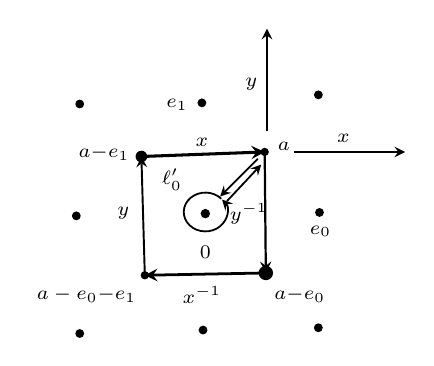
\begin{tikzpicture}[x=1.45cm,y=1.45cm,>=stealth,font=\scriptsize]
\fill (-1.10,0.96) circle (1.6pt);
\fill (-0.03,0.97) circle (1.6pt);
\fill (0.99,1.04) circle (1.6pt);
\fill (-1.13,-0.02) circle (1.6pt);
\fill (0,0) circle (1.7pt);
\fill (1.00,0.01) circle (1.6pt);
\fill (-1.10,-1.05) circle (1.6pt);
\fill (-0.02,-1.02) circle (1.6pt);
\fill (0.99,-1.00) circle (1.6pt);
\node[left] at (-0.07,0.95) {$e_1$};
\node[below] at (1.01,-0.02) {$e_0$};
\node[below] at (0,-0.20) {$0$};
\coordinate (a) at (0.52,0.54);
\coordinate (b) at (-0.56,0.50);
\coordinate (c) at (-0.53,-0.54);
\coordinate (d) at (0.53,-0.52);
\fill (a) circle (1.5pt);
\fill (b) circle (2.1pt);
\fill (c) circle (1.5pt);
\fill (d) circle (2.6pt);
\draw[->,line width=1.1pt] (b) -- (a);
\node[above] at (-0.03,0.50) {$x$};
\draw[->,line width=.7pt] (c) -- (b);
\node[left] at (-0.58,0.00) {$y$};
\draw[->,line width=1.0pt] (d) -- (c);
\node[below] at (-0.03,-0.55) {$x^{-1}$};
\draw[->,line width=.8pt] (a) -- (d);
\node at (0.38,0.00) {$y^{-1}$};
\draw[->,line width=.7pt] (0.54,0.72) -- (0.54,1.62);
\node[left] at (0.54,1.13) {$y$};
\draw[->,line width=.7pt] (0.78,0.54) -- (1.75,0.54);
\node[above] at (1.21,0.54) {$x$};
\node[right] at (0.55,0.59) {$a$};
\node[left] at (-0.58,0.53) {$a\unsure{-}e_1$};
\node[below left] at (-0.52,-0.56) {$a-e_0\unsure{-}e_1$};
\node[below right] at (0.52,-0.56) {$a\unsure{-}e_0$};
\draw[->,line width=.65pt] (0.46,0.48) -- (0.13,0.15);
\draw[->,line width=.65pt] (0.19,0.11) -- (0.49,0.43);
\draw[->,line width=.65pt] (0.14,0.13)
 arc[start angle=43,end angle=400,x radius=.19,y radius=.17];
\node[above left] at (-0.12,0.12) {$\ell'_0$};
\end{tikzpicture}}

Alors l'élément $xyx^{-1}y^{-1}$ est figuré par le chemin ci-dessus, qui est visiblement opposé au lacet ``\unsure{radiologique}'' direct de $a$ autour de l'origine $0$.
\margin{240}

\begin{center}
240\\
\texttt{https://grothendieck.umontpellier.fr}\\
Université de Montpellier, UMR CNRS 5149, Case courrier 051, Place Eugène Bataillon\\
34095 Montpellier cedex 5 - France
\end{center}
\scanpage{242}

$5^\circ$) \uline{Digression sur les} \inserted{\uline{revêtements de}} \uline{germes d'espaces.}

\margin{A) \uline{Revêtements de germes}}
\margin{ici on n'exclut \deleted{\unsure{le}} \inserted{pas le} filtre impropre $(\varnothing\in\Phi)$ correspondant au germe d'espace \uline{vide}}

Un ``germe d'espace'' est défini par un espace topologique $S$ et une \deleted{base de} filtre $\Phi$ sur $S$, un morphisme de $(S,\Phi)$ dans $(S',\Phi')$ est un élément de
\[
\text{(46)}\qquad
\varinjlim_{S_i\in\Phi}\operatorname{Hom}_{\Phi_{\unsure{S_i|S'_i}},\Phi'}(S_i,S'),
\]
où \deleted{$\Phi_{S_i}$ est} pour $S_i\in\Phi$, $\Phi_{S_i}$ est le filtre induit par $\Phi$ sur $S_i$, et $\operatorname{Hom}_{\Phi_{S_i},\Phi'}$ désigne l'ensemble des appl. continues \inserted{$f$} de $S_i$ dans $S'$ compatibles avec $\Phi_{S_i},\Phi'$, i.e. telles que $\forall S'_j\in\Phi'$, \deleted{$\unsure{f}$} on ait $f^{-1}(S'_j)\in\Phi_{S_i}$. La composition des morphismes de germes est évidente.

Un \uline{revêtement} (étale) d'un germe $(S,\Phi)$ d'espaces top. est un objet de la catégorie
\[
\text{(47)}\qquad
\underline{\mathrm{Rev}}(S,\Phi)=\varinjlim_{S_i\in\Phi}\underline{\mathrm{Rev}}(S_i);\qquad\unsure{*}
\]
\unsure{ces|les} revêtements forment une catégorie, que nous pourrions \inserted{sans doute} interpréter \inserted{(au moins dans les ``bons cas'')} comme la catégorie des revêtements d'un topos convenable (savoir le topos limite
\margin{241}

\begin{center}
241\\
\texttt{https://grothendieck.umontpellier.fr}\\
Université de Montpellier, UMR CNRS 5149, Case courrier 051, Place Eugène Bataillon\\
34095 Montpellier cedex 5 - France
\end{center}
\scanpage{243}
\mspage{769}

\margin{cela ne fait pas \unsure{aller} \unsure{loin|long} ?}

projective des \inserted{(petits)} topos étales des $S_i\in\Phi$).

Cette catégorie, ``dans les bons cas'', a tendance à être multigaloisienne, voire galoisienne.

On dit qu'un germe \deleted{\unsure{est}} d'espaces est $1$-connexe, ou simplement connexe, si le foncteur naturel

\diagram{\begin{tikzcd}[ampersand replacement=\&,column sep=large,row sep=small]
{(48)} \& (\mathrm{Ens}) \arrow[r] \& \underline{\mathrm{Rev}}(S,\Phi) \\
 \& E \arrow[r,mapsto] \& {\unsure{{}^{1}\!E_{(S,\Phi)}|\widetilde E_{(S,\Phi)}},\ \text{rev. const. de}} \\
 \& \& {\text{valeur }E}
\end{tikzcd}}

est une équivalence de catégories. Ceci signifie que

$1^\circ)$ Ce foncteur est pl. fidèle (on dit que $(S,\Phi)$ est $0$-connexe), ce qui s'exprime, si $S$ est loc. connexe, par $\forall S_i\in\Phi$, $\exists S_j\in\Phi$, $S_j\subset S_i$, tel que \inserted{$S_j\ne\varnothing$ et} $(\pi_0(S_j)\longrightarrow\pi_0(S_i))$ soit une application constante

\margin{donc ceci implique que le germe d'espaces est non vide}

$2^\circ)$ le foncteur est de plus \unsure{ess!|ess$^{\mathrm t}$} surjectif, ce qui signifie que pour tout $S_i\in\Phi$, $\exists S_j\in\Phi$, \inserted{$S_j\subset S_i$} tel que pour tte composante connexe $S_{j,\alpha}$ de $S_j$, l'hom. ext. $\pi_1(S_{j,\alpha})\longrightarrow\pi_1(S_i)$ soit triviale.

Les revêtements de germes d'espaces forment une catégorie fibrée sur celle

\margin{242}

\begin{center}
242\\
\texttt{https://grothendieck.umontpellier.fr}\\
Université de Montpellier, UMR CNRS 5149, Case courrier 051, Place Eugène Bataillon\\
34095 Montpellier cedex 5 - France
\end{center}
\scanpage{244}

des germes d'espaces. La catégorie des espaces top. \deleted{\illegible{1}} peut être considérée comme sous-catégorie pleine de celle des germes d'espaces topologiques en \unsure{associant} à tt espace $\unsure{S}$, le germe $(S,\Phi)$, où $\Phi$ est le filtre trivial sur $S$. Ceci étant, la cat. fibrée des revêtements de germes d'espaces \unsure{induit|induite} celle des rev. d'espaces topologiques.

Soit $\deleted{\unsure{\mathcal S}}\mathcal X$ un germe d'espaces tel que $\underline{\mathrm{Rev}}\mathcal X$ soit une catégorie \inserted{multi}galoisienne, \deleted{Alors} et soit $\mathcal S$ un germe d'espaces $1$-connexe, $\mathcal S\longrightarrow\mathcal X$ un morphisme. Alors on a

\diagram{\begin{tikzcd}[ampersand replacement=\&,column sep=large]
{(49)} \& \underline{\mathrm{Rev}}(\mathcal X) \arrow[r] \& \underline{\mathrm{Rev}}(\mathcal S) \& (\mathrm{Ens}) \arrow[l,"\sim"']
\end{tikzcd}}

foncteur fibre sur $\underline{\mathrm{Rev}}(\mathcal X)$, ce qui permet de définir
\[
(50)\qquad \pi_1(\deleted{\unsure{\mathcal S}}\unsure{\mathcal X},\mathcal S)
\]
comme le $\pi_1$ relatif à ce foncteur fibre. Si $\mathcal X$ est $0$-connexe donc $\underline{\mathrm{Rev}}(\mathcal X)$ est galoisienne, on aura donc, si $\Pi\simeq\pi_1(\mathcal X,\mathcal S)$, une équivalence de catégories

\margin{243}

\begin{center}
243\\
\texttt{https://grothendieck.umontpellier.fr}\\
Université de Montpellier, UMR CNRS 5149, Case courrier 051, Place Eugène Bataillon\\
34095 Montpellier cedex 5 - France
\end{center}
\scanpage{245}
\mspage{770}

\[
(51)\qquad \underline{\mathrm{Rev}}(\mathcal X)\simeq\mathrm{Ens}(\Pi).
\]

Le groupe $\pi_1(\mathcal X,\mathcal S)$ dépend fonctoriellement du triple $(\mathcal S,\mathcal X,\mathcal S\longrightarrow\mathcal X)$ i.e de la flèche $\mathcal S\longrightarrow\mathcal X$ dans la catégorie des germes d'espaces, où $\deleted{\mathcal S}$ la source $\mathcal S$ est $1$-connexe.

\unsure{Soient|Soit} $X$ un espace top., $Y$ une partie de $X$, on \uline{appelle germe de} $X$ \uline{autour de} $Y$ le germe d'espaces $(X,\Phi)$, où $\Phi$ est le filtre des voisinages de $Y$ \unsure{dans|ds} $X$, \uline{germe résiduel de $X$ autour de $Y$} le germe d'espaces $(X\setminus Y,\Phi_{X\setminus Y})$ induit sur $X-Y$ (il est vide \unsure{ssi} $Y$ est ouvert).

\margin{On a un \unsure{diagramme} de morphismes \unsure{canoniques}
\diagram{\begin{tikzcd}[ampersand replacement=\&,column sep=large,row sep=large]
\unsure{\mathrm{Germ}_{Y}(X)} \arrow[d,hook] \& \unsure{\mathrm{Gerres}_{Y}(X)} \arrow[l,hook'] \arrow[d,hook] \\
X \& X-Y \arrow[l,hook']
\end{tikzcd}}\quad (52)}

Nous utiliserons cette notion \deleted{\unsure{surtout}} dans le cas où $Y=\{x\}$, en parlant aussi de germe et germe résiduel de $X$ en $x$. (\uline{NB} le germe de $X$ en $x$ est tjrs \deleted{\unsure{simp}} $1$-connexe, mais pas le germe résiduel). Tout germe d'espaces \inserted{$(S,\Phi)$} peut s'interpréter comme germe résiduel d'un espace \deleted{$(\unsure{S},\unsure{\Phi})$} $\unsure{X}=S\cup\{\omega\}$ en un pt $\omega$ convenable \ldots

\margin{244}

\begin{center}
244\\
\texttt{https://grothendieck.umontpellier.fr}\\
Université de Montpellier, UMR CNRS 5149, Case courrier 051, Place Eugène Bataillon\\
34095 Montpellier cedex 5 - France
\end{center}
\scanpage{246}

\unsure{.} Je m'intéresse au cas où $x\in X$ admet un voisinage homéomorphe à $\mathbb R^2$ --- i.e. $X$ est une surface en $x$. Je désignerai par $\deleted{D_{X,x}^{*}}$
\[
(53)\qquad D_{X,x}^{*}\quad\text{ou}\quad D_x^{*}
\]
le germe résiduel de $X$ en $x$ (contenu dans le germe $D_{X,x}$ ou $D_x$ de $X$ en $x$).

Je m'intéresse au choix d'un \uline{rev. universel} $D_x^{*\,\sim}$ de $D_x^{*}$ --- mais pour \unsure{quoi|qui} il me faut faire une digression sur la notion abstraite de \uline{rev universel d'un germe d'espaces}.

Soit $(S,\Phi)$ un germe d'espaces. Un rev. de $(S,\Phi)$ provient d'un rev $S'_i$ d'un $S_i\in\Phi$, et définit un germe d'espaces $(S'_i,\Phi_{S'_i})$, où $\Phi_{S'_i}$ désigne l'image inverse de $\Phi_{\deleted{\unsure{S'_i}}S_i}$ dans $S'_i$. Ce germe d'espaces \inserted{au dessus de $\mathcal S=(S,\Phi)$} (à isom unique près de germes) ne dépend pas du choix de $S_i$, $S'_i$, mais seulement de l'élément de $\underline{\mathrm{Rev}}(\mathcal S)$. On trouve ainsi un foncteur canonique

\margin{245}

\begin{center}
245\\
\texttt{https://grothendieck.umontpellier.fr}\\
Université de Montpellier, UMR CNRS 5149, Case courrier 051, Place Eugène Bataillon\\
34095 Montpellier cedex 5 - France
\end{center}
\scanpage{247}
\mspage{771}

\diagram{\begin{tikzcd}[ampersand replacement=\&,column sep=large]
{(54)} \& \underline{\mathrm{Rev}}(\mathcal S) \arrow[r] \& {(\unsure{\mathrm{Germesp}})/\mathcal S}
\end{tikzcd}}

qui est \uline{pleinement fidèle}. Un germe d'espaces $\mathcal S'$ au dessus de $\mathcal S$ est dit \deleted{\unsure{le}} un \uline{revêtement étale} \uline{de} $\mathcal S$, s'il est dans l'image essentielle. Ainsi la cat. $\underline{\mathrm{Rev}}(\mathcal S)$ des revêtements étales du germe d'espaces $\mathcal S$ est équivalente à la sous-catégorie pleine de la \deleted{\unsure{g}} cat. des germes d'espaces, au dessus du germe $\mathcal S$, \deleted{qui} formée des rev. étales dudit germe $\mathcal S$.

Supposons \deleted{que} \unsure{toujours|tjrs} que la cat. $\underline{\mathrm{Rev}}(\mathcal S)$ est \deleted{\unsure{g}} multigaloisienne. Les objets $1$-connexes sont appelés des rev. universels de $\mathcal S$ --- \deleted{si $\underline{\mathrm{Rev}}(\mathcal S)$ est galoisienne,} ils forment un groupoïde, connexe ssi $\underline{\mathrm{Rev}}(\mathcal S)$ est galoisienne i.e. ssi le germe $\mathcal S$ est $0$-connexe. Les \unsure{rev!|rev.} universels de $\mathcal S$ peuvent s'interpréter comme des germes d'espaces. Soit $\widetilde{\mathcal S}$ un tel rev. universel, alors $\widetilde{\mathcal S}$ est bel et bien un germe d'espaces \unsure{$1$-connexe|$1$. connexe}, et $\widetilde{\mathcal S}\longrightarrow\mathcal S$ permet de définir $\pi_1(\mathcal S,\widetilde{\mathcal S})$. Ceci posé, on a un iso. can.
\[
(\unsure{55|53})\qquad \pi_1(\mathcal S,\widetilde{\mathcal S})\simeq\mathrm{Aut}_{\underline{\mathrm{Rev}}(\mathcal S)}(\widetilde{\mathcal S})
\]

\margin{Ce qui exprime que $\pi_1(\mathcal S,\widetilde{\mathcal S})$ n'est autre que le $\pi_1$ de la cat. \inserted{multi}galoisienne ``abstraite'' $\underline{\mathrm{Rev}}(\mathcal S)$, ``calculé'' en l'élément $1$-connexe $\widetilde{\mathcal S}$.}

\margin{\figure{\begin{tikzpicture}[x=1cm,y=1cm]
\draw (0,0) -- (0.18,0.43);
\draw (0.04,0.10) -- (0.14,0);
\end{tikzpicture}}}

\margin{246}

\begin{center}
246\\
\texttt{https://grothendieck.umontpellier.fr}\\
Université de Montpellier, UMR CNRS 5149, Case courrier 051, Place Eugène Bataillon\\
34095 Montpellier cedex 5 - France
\end{center}
% ===== LM_C4-248-266: first pass, with mechanical fixes =====
\scanpage{248}
\margin{B) \uline{Cas des surfaces ponctuées}}
\deleted{\unsure{Bref.}}

Ceci dit, revenons à la situation de (53), d'un espace topologique $X$, et d'un $x\in X$ tel que $X$ soit une surface en $x$. Alors la catégorie \deleted{des \unsure{rev.}}
\[
\underline{\mathrm{Rev}}(D_x^*)
\]
est une catégorie galoisienne, \inserted{abélienne,} dont le groupe fondamental s'identifie \unsure{canoniquement} au module d'orientation $\overline T_x$ de $X$ en $x$
\[
(56)\qquad \pi_1(D_x^*)\overset{\mathrm{def}}=\pi_1(\underline{\mathrm{Rev}}(D_x^*))\simeq\overline T_x.
\]
Ceci provient du fait que le germe $D_x^*$ \deleted{\unsure{est} \illegible{1}} \inserted{admet une ``base''} formée d'espaces $D_{x,i}^*$ \deleted{\unsure{isomorphes à}} \inserted{\unsure{provenant}} des \uline{disques} de centre $x$, et les $\pi_1$ desdits disques \unsure{forment} un syst. projectif constant\ldots

Ainsi les rev. universels $D_x^{*\sim}$ de $D_x^*$ forment un groupoïde connexe, de \unsure{groupoïde|groupe} fondamental $\deleted{\unsure{\mathbb{Z}}}\,\overline T_x$.

Choisissons donc un tel $D_x^{*\sim}$, et considérons les morphismes composés
\scanpage{249}
\mspage{772}
\diagram{\begin{tikzcd}
D_x^{*\sim}\arrow[r] & D_x^*\arrow[r,hook] & X-\{x\}
\end{tikzcd}}
- plus généralement, soit $S$ une partie de $X$, contenant $x$ comme pt isolé (p. ex. une partie discrète de $X$), de sorte qu'on a
\diagram{\begin{tikzcd}
(57)\qquad D_x^*\arrow[r,hook] & U\overset{\mathrm{def}}=X\setminus S
\end{tikzcd}}
et considérons les composés
\diagram{\begin{tikzcd}
(58)\qquad D_x^{*\sim}\arrow[r] & D_x^*\arrow[r,hook] & U.
\end{tikzcd}}
Si $\underline{\mathrm{Rev}}(U)$ est \unsure{multigaloisienne} (p. ex. $U$ \inserted{loc} $\unsure{0|1}$-connexe), alors on peut donc considérer le groupe fondamental correspondant de $U$
\[
(59)\qquad \pi_1(U,D_x^{*\sim}),
\]
je vais définir un \uline{hom} \uline{canonique}
\diagram{\begin{tikzcd}[column sep=large]
(60)\qquad \unsure{k_x|\kappa_x}:\overline T_x\arrow[r] &
\underbrace{\pi_1(U,D_x^{*\sim})}_{\inserted{\begin{gathered}
\simeq\operatorname{Aut}\text{ du foncteur}\\
\text{fibre }\underline{\mathrm{Rev}}(U)\longrightarrow\underline{\mathrm{Rev}}(D_x^{*\sim})\\
\text{sur }\underline{\mathrm{Rev}}(U)
\end{gathered}}},
\end{tikzcd}}
on peut le décrire p. ex. comme
\diagram{\begin{tikzcd}
(61)\qquad \pi_1(D_x^*,D_x^{*\sim})\arrow[r]\arrow[d,phantom,"\simeq" description,sloped] & \pi_1(U,D_x^{*\sim})\\
\overline T_x &
\end{tikzcd}}
\scanpage{250}
induit par l'inclusion
\diagram{\begin{tikzcd}
D_x^*\arrow[r,hook] & U
\end{tikzcd}}
ou encore, \deleted{\unsure{par}} en termes d'\unsure{autom.} d'un foncteur fibre, comme l'\deleted{\unsure{hom}}opération de $\overline T_x$ sur
\[
\Gamma\bigl(D_x^{*\sim},\underbrace{U'\mathbin{\times}_{\deleted{\unsure{D}}U}D_x^{*\sim}}_{\inserted{U'_{D_x^{*\sim}}}}\bigr)
\]
provenant des opérations de $\overline T_x$ sur $D_x^{*\sim}$.
\diagram{\begin{tikzcd}[column sep=small,row sep=small]
& U'_{D_x^{*\sim}}\arrow[dl]\arrow[dr] &\\
D_x^{*\sim}\arrow[dr] && U'\arrow[dl]\\
& U &
\end{tikzcd}}
\deleted{\illegible{1} \uline{NB} \unsure{Chaque fois}}

Supposons qu'on ait déjà choisi \inserted{par ailleurs} un groupe fondamental \inserted{$\pi_1(U,\widetilde U)=\pi$} de $U$, par le choix d'un pt base, ou, plus \unsure{généralement}, d'un rev. universel $\widetilde U$ de $U$.
Pour le comparer avec $\pi_1(U,\deleted{\unsure{S}}D_x^{*\sim})$, on choisira donc un ``chem. de \unsure{domin.}'' de $D_x^{*\sim}/U$ \unsure{à|:} $\widetilde U/U$, i.e. un isomorphisme
\diagram{\begin{tikzcd}
(62)\qquad \widetilde U\arrow[r,"\sim"] & \mathrm{Revuni}(U,D_x^{*\sim})
\end{tikzcd}}
(rev. universel de $\deleted{\unsure{\widetilde U}}U$ défini par le foncteur fibre
\diagram{\begin{tikzcd}
& \underline{\mathrm{Rev}}(U)\arrow[r] & \underline{\mathrm{Rev}}(D_x^{*\sim})\\
\inserted{\unsure{U}}\arrow[ur,bend right] &&
\end{tikzcd}}
\margin{\uline{NB} si \deleted{\illegible{1}} $D_x^{*\sim}$ défini par un rev. universel $D_{x,i}^{*\sim}$ d'un disque \unsure{épointé} $D_{x,i}^*$, et si $\widetilde y\in D_{x,i}^{*\sim}$, $\widetilde z\in\widetilde U$, $y,z$ les images dans $U$, alors
\[
\deleted{\unsure{D}}\mathrm{Revuni}(U,D_x^{*\sim})\simeq\mathrm{Revuni}(U,y)
\]
et $\widetilde U\simeq\mathrm{Revuni}(U,z)$ : le choix de (62) \unsure{équivaut à} celui d'un \unsure{chemin} de $y$ à $z$ ($\unsure{U}$ \unsure{loc.} \unsure{1-connexe}).}
\scanpage{251}
\mspage{773}
(l'indétermination est \unsure{mod} un \deleted{\unsure{autom.}} \inserted{élément} \deleted{\unsure{int.}} de $\pi$, ou de $\pi_1(U,D_x^{*\sim})$) qui induit un isom
\diagram{\begin{tikzcd}
(63)\qquad \unsure{\pi_s|\pi}=\pi_1(U,\widetilde U)\arrow[r,leftrightarrow,"\sim"] & \pi_1(U,D_x^{*\sim})
\end{tikzcd}}
(qui est changé par un autom. intérieur, quand on \unsure{change|compose} (62) par un élément de $\pi$).

Composant (63) et (60), on trouve donc un hom
\diagram{\begin{tikzcd}
(64)\qquad \overline T_x\arrow[r] & \pi=\pi_1(U,\widetilde U),
\end{tikzcd}}
qui dépend du choix de (62) -- et qui, indépendamment de ce choix, définit un \uline{hom} \uline{ext.} bien déterminé -- qui n'est autre que l'hom ext.
\diagram{\begin{tikzcd}
(65)\qquad \pi_1(D_x^*)\arrow[r]\arrow[d,phantom,"\simeq" description,sloped] & \pi_1(U)\arrow[d,phantom,"\simeq" description,sloped].\\
\overline T_x & \pi
\end{tikzcd}}

\margin{C) \uline{Relation avec} \uline{germes d'arcs} (\unsure{jouant} le rôle \deleted{\unsure{origine}} de ``\unsure{pts|pt} base'')}
Je vais décrire une façon commode de fixer un rev. universel $D_x^{*\sim}$ de $D_x^*$, par un \uline{germe} \uline{d'arc de courbe} \inserted{\uline{de} $X$,} \uline{sortant}
\scanpage{252}
de $x$. De façon générale, soit $\unsure{I|\overline I}=[0,1]$, et $[\unsure{I|\overline I}]$ le germe \unsure{résiduel} de $\unsure{I|\overline I}$ en $0$. \deleted{Si $X$ est un espace} \inserted{C'est évidemment un \uline{germe} \uline{1-connexe}.}

\margin{Plutôt que de \uline{\unsure{paramétrer}} par des germes de \unsure{voisinages} de $0$ dans $[0,1]$, il serait plus commode pour la suite de définir un germe d'arc de $X$ sort. de $x$ comme un germe de \unsure{sous-ensemble} de $X$ en $x$, satisfaisant à \unsure{certaines} propriétés\ldots.}

Si $X$ est un espace top. et $x\in X$, on appelle germe d'arc de courbe \deleted{de} $X$ sortant de $x$, les morphismes
\diagram{\begin{tikzcd}
(66)\qquad [\unsure{I|\overline I}]\arrow[r,"\gamma"] & \unsure{\mathrm{germ\,rés}}_x(X)\overset{\mathrm{def}}=D_x^*
\end{tikzcd}}
\[
\inserted{\underbrace{D_{X,x}^*}}
\]
du germe $[\unsure{I|\overline I}]$ dans le germe \unsure{résiduel} de $X$ en $x$. Un tel germe est donc décrit par une application continue d'un intervalle $[0,\varepsilon]$ ($0<\varepsilon\leq1$)
\diagram{\begin{tikzcd}
(67)\qquad [0,\varepsilon]\arrow[r,"{\varphi\,\deleted{\unsure{\gamma}}}"] & X
\end{tikzcd}}
telle que l'on ait
\[
(68)\qquad\left\{\begin{array}{l}
\varphi(0)=x\\
\varphi(t)\neq x\quad\text{si }t\in]0,\varepsilon]
\end{array}\right.\quad.
\]
Dans le cas qui nous intéresse ($X$ une surface au voisinage de $x$, donc $\underline{\mathrm{Rev}}(D_x^*)$ \deleted{\unsure{galoisienne}} \inserted{galoisienne} abélienne de groupe $\overline T_x$), on peut utiliser cet hom pour définir un foncteur fibre sur $D_x^*$
\diagram{\begin{tikzcd}
(69)\qquad \underline{\mathrm{Rev}}(D_x^*)\arrow[r] & \underline{\mathrm{Rev}}([\unsure{I|\overline I}]) & (\mathrm{Ens})\arrow[l,"\sim"']
\end{tikzcd}}
\scanpage{253}
\mspage{774}

d'où un rev. universel
\[
\tag{70}
D_x^{*\sim}\overset{\mathrm{d\acute ef}}{=}
\mathrm{Rev\,uni}\bigl(D_x^*,([\unsure{I|\overline I}],\varphi)\bigr).
\]

Bien entendu, on aura une factorisation
\diagram{\begin{tikzcd}[column sep=large]
[\unsure{I|\overline I}] \arrow[r] \arrow[rr,bend right=18,"\varphi"'] &
D_x^{*\sim} \arrow[r] & D_x^*\;( \arrow[r,hook] & U)
\end{tikzcd}}

donc on a un \unsure{iso can.}
\[
\tag{71}
\mathrm{Rev\,uni}(U,D_x^{*\sim})\simeq
\mathrm{Rev\,uni}(U,[\unsure{I|\overline I}]),
\]
où $I$ est considéré comme un germe $1$-connexe sur $U$ par le morphisme composé
\diagram{\begin{tikzcd}
{[\unsure{I|\overline I}]} \arrow[r] & D_x^* \arrow[r] & U.
\end{tikzcd}}

Donc on a
\diagram{\begin{tikzcd}[column sep=large]
{\text{(72)}\quad \pi_1(U,D_x^{*\sim})=\pi_1(U,[\unsure{I|\overline I}])} &
\overline T_x. \arrow[l,"K_x"']
\end{tikzcd}}

\margin{D) \uline{Relation avec structure différentielle}}
Lorsque $X$ est muni d'une structure différentiable au voisinage de $x$, on dit qu'un germe de courbe dans $X$ sortant de $x$ est \uline{différentiable}, si \unsure{le|l'} \deleted{application}\inserted{germe} d'application continue
\diagram{\begin{tikzcd}
I \arrow[r] & X
\end{tikzcd}}
qui le définit est différentiable, \deleted{\unsure{Prenons|Pour cela}}\inserted{et de plus}
\scanpage{254}

l'application tangente à l'origine, \deleted{\illegible{2} \unsure{conduit} un \unsure{hom.}}
\diagram{\begin{tikzcd}
{\text{(73)}\quad\mathbb R} \arrow[r] & \mathrm{Tang}_x(X),
\end{tikzcd}}
est injective. Alors l'image de $\mathbb R^+$ est une demi-droite homogène dans l'espace tangent à $X$ en $x$, qu'on appelle la \uline{demi-tangente} du germe d'arc de courbe envisagé en $x$.

Revenant pour un moment au cas purement topologique, nous allons considérer l'ens $\unsure{\mathrm{Germarc}|\mathrm{Courarc}}(X,x)$ des germes d'arcs de $X$ sortant de $x$, comme l'ens des objets d'un groupoïde (le groupoïde fondamental local de $X$ en $x$), en prenant comme morphismes de $\gamma$ en $\gamma'$ \deleted{\unsure{un|les}} les isomorphismes de \deleted{$\mathrm{Rev\,uni}(D_x^*,\gamma)$} $D_{x,\gamma}^{*\sim}$ sur $D_{x,\gamma'}^{*\sim}$
\[
\tag{74}
\mathrm{Isom}(\gamma,\gamma')\overset{\mathrm{d\acute ef}}{=}
\mathrm{Isom}_{D_x^*}(D_{x\gamma}^{*\sim},D_{x,\gamma'}^{*\sim}).
\]
On trouve donc \inserted{par construction} une équivalence de \deleted{catégories (de} groupoïdes connexes
\diagram{\begin{tikzcd}[column sep=large]
{\text{(75)}\quad\uline{\unsure{\mathrm{Germarc}|\mathrm{Courarc}}}(X,x)} \arrow[r] &
\uline{\mathrm{Rev\,uni}}(D_x^*).
\end{tikzcd}}
\scanpage{255}
\mspage{775}

Soit d'autre part, dans le cas où $X$ est diff. en $x$, \deleted{\unsure{Germ}}
\[
\tag{76}
\uline{\unsure{\mathrm{Germarc\,diff}|\mathrm{Courarc\,diff}}}(X,x)
\]
la sous-catégorie pleine de \deleted{$\unsure{\mathcal C_x|\mathcal G_x}$} $\uline{\unsure{\mathrm{Germarc}|\mathrm{Courarc}}}(X,x)$ formée des germes d'arc différentiables. Soit $\mathbb S_x$ \inserted{$\simeq\mathbb S^1$} \deleted{la catégorie}\inserted{l'}espace des demi-droites de l'espace Tangent $\mathrm{Tang}_x(X)$
\[
\tag{77}
\mathbb S_x=
\begin{array}{l}
\inserted{\text{espace des}}\\
\text{Demi droites}\\
\text{de }\mathrm{Tang}_x(X)
\end{array}
\simeq\mathbb S^1,
\]
et considérons le groupoïde fondamental
\diagram{\begin{tikzcd}[column sep=large]
{\text{(78)}\quad\Pi_1(\mathbb S_x)} \arrow[r,"\approx"] & \uline{\mathrm{Rev\,uni}}(\mathbb S_x).
\end{tikzcd}}

\margin{\figure{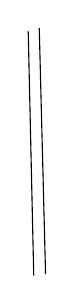
\begin{tikzpicture}[x=1cm,y=1cm]
\draw (0,0) -- (0.07,-3.1);
\draw (0.14,0.04) -- (0.22,-3.08);
\end{tikzpicture}}}
Je vais définir une équivalence de catégories
\diagram{\begin{tikzcd}[column sep=large,row sep=large]
{\text{(79)}\quad\uline{\unsure{\mathrm{Germarc\,diff}|\mathrm{Courarc\,diff}}}(X,x)} \arrow[r,"\approx"] \arrow[d,"\approx"{rotate=90}] &
\Pi_1(\mathbb S_x) \arrow[d,"\approx"{rotate=90}]\\
\uline{\mathrm{Rev\,uni}}(D_x^*) & \uline{\mathrm{Rev\,uni}}(\mathbb S_x)
\end{tikzcd}}
qui, sur les ensembles d'objets, soit l'application \unsure{associant} à $\forall$ germe d'arc différentiable en $x$ sa demi-\uline{tangente}. Il s'agit donc, si $\gamma,\gamma'$ sont deux tels arcs, correspondant à des demi-tangentes $\Delta,\Delta'$, de définir une bijection canonique
\scanpage{256}

\margin{\figure{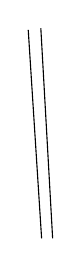
\begin{tikzpicture}[x=1cm,y=1cm]
\draw (0,0) -- (0.17,-2.65);
\draw (0.16,0.02) -- (0.31,-2.65);
\end{tikzpicture}}}
\diagram{\begin{tikzcd}[column sep=huge,row sep=large]
{\text{(80)}\quad\mathrm{Isom}(\gamma,\gamma')} \arrow[r,"\sim"] \arrow[d,equal,"\mathrm{d\acute ef}"] &
\mathrm{Isom}_{\Pi_1\mathbb S_x}(\Delta,\Delta') \arrow[d,equal,"\mathrm{d\acute ef}"]\\
\mathrm{Isom}(D_{x,\gamma}^{*\sim},D_{x,\gamma'}^{*\sim}) &
{\begin{array}{l}
\text{classes de chemins}\\
\text{dans }\unsure{\mathbb S_x^*|\mathbb S_x}\text{ de }\Delta\\
\text{à }\Delta'
\end{array}}
\end{tikzcd}}

\deleted{\illegible{1}}
Au lieu de définir directement la bijection (80), je vais définir plutôt un foncteur (qui sera une équivalence de catégories)
\diagram{\begin{tikzcd}[column sep=large]
{\text{(81)}\quad\Theta:\Pi_1(\mathbb S_x)} \arrow[r,"{(\deleted{\unsure{\to|\sim}}\approx)}"] &
\uline{\mathrm{Rev\,uni}}(D_x^*),
\end{tikzcd}}

Soit \deleted{$\mathcal A$}
\[
\tag{82}
\left\{
\begin{array}{l}
\mathcal A_x\text{ ens des parties }\inserted{\text{fermées}}\text{ }1\text{-connexes de }\mathbb S_x\\
(\text{i.e. des }\uline{\text{arcs}}\text{ de cercle dans }\mathbb S_x,\\
\quad\unsure{\text{pouvant}}\text{ être réduits }\unsure{\text{à}}\text{ des pts,}\\
\quad\text{mais }\ne\mathbb S_x)
\end{array}
\right.
\]
c'est un ensemble ordonné, \unsure{et on|donc} \deleted{l'ensemble} définit une catégorie ordonnée $\uline{\mathcal A}_x$ (les objets sont les $\in\mathcal A_x$, les flèches sont les inclusions) --- et on sait que le groupoïde enveloppant \inserted{$\uline{\mathrm{Gr}}(\uline{\mathcal A}_x)$} de cette catégorie ordonnée est canoniquement équivalent à $\Pi_1(\mathbb S_x)$,
\scanpage{257}
\mspage{776}

de façon précise, soit \deleted{$\unsure{\uline{\mathcal A}_{0x}|\uline{\mathcal A}_x}$}\inserted{$\uline{\mathrm{Gr}}_0(\uline{\mathcal A}_x)$} la sous-catégorie pleine de $\uline{\mathrm{Gr}}(\uline{\mathcal A}_x)$ (dont l'ens des objets est $\mathcal A_x$) dont les objets soient les arcs \uline{ponctuels}, \& on a alors une équivalence canonique
\diagram{\begin{tikzcd}[column sep=large]
{\text{(83)}\quad\uline{\mathrm{Gr}}_0(\uline{\mathcal A}_x)} \arrow[r,"\approx"] & \Pi_1(\mathbb S_x)
\end{tikzcd}}
qui sur les objets se réduit à $\{a\}\longmapsto a$, et qui, pour tout arc \deleted{$\unsure{\mathbb S|\xi}$} $A$ d'extrémités $a,b$, d'où des isom d'inclusion \unsure{ds|dans} $\uline{\mathrm{Gr}}(\mathcal A_x)$
\diagram{\begin{tikzcd}[column sep=normal,row sep=large]
{\text{(84)}\quad\raisebox{-1.6em}{$\left\{\rule{0pt}{3.2em}\right.$}} &
a \arrow[r,"\sim"] & A & b \arrow[l,"\sim"'] & \\
& \text{d'où}\quad a \arrow[rr,"\sim"] & & b & \text{dans }\uline{\mathrm{Gr}}(\mathcal A_x)
\end{tikzcd}}
associe à cette flèche $a\overset{\sim}{\longrightarrow}b$ de $\uline{\mathrm{Gr}}_0(\mathcal A_x)$ la flèche de $\Pi_1(\mathbb S_x)$, définie par l'arc $A$ considéré comme chemin de $a$ en $b$.

Ainsi, pour $\forall$ groupoïde $\mathcal G$, la donnée d'un foncteur
\diagram{\begin{tikzcd}[column sep=large]
{\text{(85)}\quad\Psi:\Pi_1(\mathbb S_x)} \arrow[r] & \mathcal G
\end{tikzcd}}
équivaut à la donnée d'un foncteur
\scanpage{258}
\[
\tag{86}
\Psi : \underline{\mathcal A}_x \longrightarrow \mathcal G
\]
et (85) est une équivalence de cat. ssi
$\mathcal G$ est \deleted{\unsure{connexe}} connexe et
\deleted{\unsure{le}} son $\unsure{\pi_1|\Pi_1}$ est $\simeq\mathbb Z$, et si, pour
\deleted{\unsure{un $x$ de}}\inserted{un couple $(a,b)$ de}
pts $a,b$ distincts de $\unsure{\mathbb S_x}$, définissant deux arcs $A$ et $B$
d'extrémités $a,b$, \deleted{de}considérant l'autom de $a$ dans
$\underline{\mathrm{Gr}}_0(\mathcal A_x)$ i.e. dans
$\underline{\mathrm{Gr}}(\mathcal A_x)$, composé de
\[
\tag{86bis}
\diagram{\begin{tikzcd}[column sep=small]
\{a\} \arrow[r,"\sim"] & A & \{b\} \arrow[l,"\sim"'] \arrow[r,"\sim"] & B & \{a\} \arrow[l,"\sim"']
\end{tikzcd}}
\]
l'autom correspondant de $\Psi(\{a\})$ dans $\mathcal G$
soit un \uline{générateur} de $\mathrm{Aut}_{\mathcal G}(\Psi(\{a\}))$.

Nous allons donc définir un foncteur
\[
\tag{87}
\underline{\mathcal A}_x \longrightarrow
\underline{\mathrm{Revuni}}(D_x^*)
\]
\deleted{et} (satisfaisant la condition supplémentaire énoncée).
Pour définir un tel foncteur, il suffit de définir un foncteur
\[
\tag{88}
\underline{\mathcal A}_x \longrightarrow
\begin{gathered}
\text{catégorie des germes 1-connexes}\\
\text{d'espaces, \unsure{au|en} dessus du}\\
\text{germe }D_x^*
\end{gathered}
\]
\scanpage{259}
\mspage{777}
en composant ce foncteur avec le foncteur
\[
\tag{89}
\begin{gathered}
\text{cat. des germes 1-conn.}\\
\text{d'espaces \unsure{au|en} dessus}\\
\text{du germe }D_x^*
\end{gathered}
\longrightarrow \underline{\mathrm{Revuni}}(D_x^*).
\]
En fait, (88) \unsure{va associer|on associe} à $\forall\ A\in
\deleted{\unsure{\mathcal E}}\mathcal A_x$ un
\deleted{germe de \unsure{sous-espace} de $X$ en $x$, dont}
\inserted{filtre sur $X-x$ tendant vers $x$, dont}
on prendra le germe \deleted{\unsure{résiduel}}.

\deleted{\unsure{Les demi-droites}}
\inserted{Les éléments \inserted{$A$} de}
$\mathcal A_x$ s'identifient évidemment aux \uline{cônes}
\deleted{\unsure{ouverts}}\inserted{fermés $C$}
de $\mathrm{Tang}_x(X)$, \deleted{\unsure{disti}}
distincts de $\{0\}$ et de l'espace
\inserted{\unsure{tang$^{\mathrm t}$|tangent}} $\forall$ entier.
\deleted{\unsure{Soit $C$ un}}
\inserted{Soit $\unsure{C\mathcal A_x|C\in\mathcal C\mathcal A_x}$ l'un de ces cônes.}
Considérons un isom local
\deleted{\unsure{un}}
\[
\tag{90}
f:(\mathrm{Tang}_x(X),0)\deleted{\unsure{\&}}
\xrightarrow{\sim}(X,x),
\]
\deleted{dont l'appl.}
\inserted{dont l'appl.} tangente est l'identité.
\deleted{Lorsque} Si $C$ est un cône $\in\mathcal C\mathcal A_x$,
son image par un tel isom. dépend du choix de l'iso. local envisagé.
Mais considérons la \deleted{\unsure{famille|ensemble des}}
\inserted{base de filtre}
\deleted{\unsure{arcs}}\inserted{des} cônes
\inserted{$C'\in\mathcal C\mathcal A_x$} contenant
\deleted{$\unsure{\in}$} $C$ \uline{strictement}
(i.e. correspondant à des arcs $A'$ qui sont des \uline{voisinages}
de $A$, ou encore tels que $C'-\{0\}$ soit un voisinage de
$C\setminus\{0\}$), alors le
\scanpage{260}
\deleted{germe d'espace défini par la base}
\inserted{l'image par (90) \deleted{\unsure{de cette}}
\inserted{du filtre défini par la} base de}
filtre sur $\mathrm{Tang}_x(X)$ formé des
$V\cap(C'\setminus\{0\})$ \unsure{, où|:} $V$
parcourant les voisinages de $0$ dans $\mathrm{Tang}_x(X)$,
est un filtre sur $X\setminus\{x\}$ qui ne dépend pas du choix de $f$,
et qui tend vers $x$, donc définit un germe d'espace
\inserted{$\widetilde A$ ou $\widetilde C$}
au dessus de \deleted{$\unsure{X_x|X}$} $D_x^*$.
Ce germe d'espace, \deleted{\unsure{est é|et il}}
isom. au germe d'espace défini par $\mathrm{Tang}_x(X)$ muni du filtre
de base les $V\cap(C'-\{0\})$ --- où on peut prendre des $V$
convexes fermés \unsure{simétriques|symétriques}, donc
$V\cap(C'-\{0\})$ contractibles --- est évidemment 1-connexe.
Pour $A$ i.e. $C$ variable \unsure{i.e.} pour $A_1\subset A_2$
i.e. $C_1\subset C_2$ on a la relation correspondante d'inclusion
\inserted{\deleted{$\unsure{A}$}
\diagram{\begin{tikzcd}
\widetilde C_1 \arrow[r] & \widetilde C_2
\end{tikzcd}}}
sur les germes d'espaces dans $D_x^*$.
On trouve donc bien (88), d'où (87)\inserted{et (81)}, et on vérifie
que ce dernier est bien une équivalence de \deleted{catégories}
groupoïdes, via la \unsure{vérification|vérific$^{\mathrm t}$}
\deleted{\unsure{par}} \unsure{explicitée|explicité} plus haut ((86bis)).
\scanpage{261}
\mspage{778}
Considérons maintenant, à nouveau, un arc différentiable $\gamma$ dans $X$
sortant de $x$, et sa demi-tangente $\Delta$.
Alors $\{\Delta\}\in\mathcal A_x$, et on peut considérer le germe
d'espace $\{\Delta\}^{\sim}$ au dessus de $D_x^*$.
On a \inserted{\unsure{les|des}} deux morphismes d'inclusion canoniques
\[
\tag{91}
\diagram{\begin{tikzcd}
\gamma \arrow[r,hook] & \{\Delta\}^{\sim} \arrow[r,hook] & D_x^*
\end{tikzcd}}
\]
et on en déduit un isom. canonique
\[
\tag{92}
\diagram{\begin{tikzcd}[column sep=large]
\mathrm{Revuni}(D_x^*,\gamma) \arrow[r,phantom,"\simeq"] \arrow[d,equal,"\mathrm{déf}"]
& \mathrm{Revuni}(D_x^*,\{\Delta\}^{\sim}) \arrow[d,equal,"\mathrm{déf}"] \\
D_{x,\gamma}^{*\sim} & \Theta(\Delta)
\end{tikzcd}}
\]
Si $\gamma'$ est un autre arc diff. en $x$, correspondant à la demi-tangente
$\Delta'$, on a donc
\[
D_{x,\gamma}^{*\sim}\simeq\Theta(\Delta),\qquad
D_{x,\gamma'}^{*\sim}=\Theta(\Delta')
\]
d'où
\[
\diagram{\begin{tikzcd}[column sep=large,row sep=large]
\mathrm{Isom}(D_{x,\gamma}^{\unsure{*}\sim}\unsure{\}},D_{x,\gamma'}^{*\sim})
\arrow[r,phantom,"\simeq"] \arrow[d,equal,"\mathrm{déf}"]
& \mathrm{Isom}(\Theta(\Delta),\Theta(\Delta')) \\
\mathrm{Isom}(\gamma,\gamma')
& \mathrm{Isom}_{\Pi_1(\mathbb S_x)}(\Delta,\Delta')
\arrow[u,"\sim","\Theta"']
\end{tikzcd}}
\]
ce qui est la \deleted{\unsure{bonne}} bijection (80) cherchée.

\deleted{Soit} En résumé, on a un diagramme ess. comm. d'équivalences
de groupoïdes
\scanpage{262}
\[
\tag{93}
\diagram{\begin{tikzcd}[column sep=huge,row sep=huge]
\underline{\mathrm{germesdiff}}(X,x)
\arrow[r,"{\substack{\gamma\longrightarrow\underline\Delta(\gamma)\\\approx}}"]
\arrow[d,"\approx","{\substack{\gamma\mapsto\mathrm{Revuni}(D_x^*,\gamma)\\=D_{x,\gamma}^{*\sim}}}"']
& \Pi_1(\mathbb S_x)
\arrow[d,"{\approx\quad a\mapsto\mathrm{Revuni}(\mathbb S_x,\cdot)}"]
\arrow[dl,dashed,"{\Theta\ \approx}"'] \\
\underline{\mathrm{Rev.uni.}}(D_x^*) \arrow[r,"\approx"]
& \mathrm{Revuni.}(\mathbb S_x)
\end{tikzcd}}
\]
\margin{Bien sûr, la difficulté ici provenait du fait qu'on n'avait pas
de morphisme direct entre le germe $D_x^*$, et l'espace $\mathbb S_x$...}

\unsure{Le} seul foncteur qui n'ait pas encore été explicité est le foncteur
\[
\tag{94}
\diagram{\begin{tikzcd}[column sep=small,row sep=small]
\underline{\mathrm{Revuni}}(D_x^*)
\arrow[rr,"\approx"] \arrow[dr,dashed,"{\Theta^{-1}}"']
& & \mathrm{Revuni}(\mathbb S_x) \\
& \Pi_1(\mathbb S_x) \arrow[ur,"{\mathrm{can}}"'] &
\end{tikzcd}}
\]
défini comme composé de $\Theta^{-1}$ avec le foncteur can.
$\Pi_1(\mathbb S_x)\longrightarrow\mathrm{Rev.uni.}(\mathbb S_x)$.

Finalement, dans ces considérations de géométrie topologique différentielle,
la construction-clef est celle du foncteur $\Theta$ (81).
Nous avons pris quelque peine à le définir de façon invariante.
Dans le cas où on dispose d'un iso local
\[
\tag{90}
f:\bigl(\underbrace{\mathrm{Tang}_x(X)}_{V},0\bigr)\longrightarrow(X,x),
\]
la construction de \unsure{ce|---} $\Theta$ peut s'expliciter comme
une construction canonique dans un espace vectoriel $V$.
Toute demi-droite hom.
\scanpage{263}
\mspage{779}

$\Delta$ de $V$ définit un germe d'arc (\unsure{diff.}) de $V$ sortant de $0$, d'où un rev. universel correspondant $D_{V,0;\Delta}^{*\sim}$ de $D_{V,0}^{*}$, donc un rev. universel $D_{x,\Delta}^{*\sim}$ de $D_x^*$.
Il faut voir comment ce $D_{x,\Delta}^{*\sim}$ dépend ``continûment'' de $\Delta$, et ce qui revient au $\overline{\mathrm m}$, comment le rev. universel $V_{\Delta}^{*\sim}$ de $V^*=V\setminus\{0\}$ dépend continûment de $\Delta$, ce qui est tout à fait \unsure{standard}\unsure{...}.

Soit maintenant \inserted{$\unsure{u|\varphi}$} \unsure{un} un \deleted{difféomorphisme}\inserted{\unsure{automorphisme}} de $X$, fixant $x$, et différentiable en $x$. On a donc \deleted{\unsure{des}} \unsure{autom.} induits \deleted{de}
\[
\tag{\unsure{95|94}}
{}^{\unsure{u|\varphi}}D_x^*\quad\text{autom. de }D_x^*,\qquad
{}^{\unsure{u|\varphi}}\mathbb S_x\quad\text{autom. de }\mathbb S_x.
\]

Considérons d'autre part un rev. universel $\widetilde{\mathbb S}_x$ de $\mathbb S_x$, et soit $D_x^{*\sim}$ un rev. universel de $D_x^*$ associé, grâce à l'équiv. (94). Je dis qu'on a alors une
\scanpage{264}

bijection canonique
\[
\tag{96}
\diagram{\begin{array}{c@{\qquad}c@{\qquad}c}
\text{ens des relèvements}&\simeq&\text{ens des relèvements}\\
\text{de }{}^uD_x^*\text{ en un}&&\text{de }{}^u\mathbb S_x\text{ en un}\\
\text{autom }{}^uD_x^{*\sim}\text{ du}&&\text{autom }{}^u\mathbb S_x^\sim\text{ de}\\
\text{germe }D_x^{*\sim}&&\mathbb S_x^\sim
\end{array}},
\]
\margin{la construction (96) sera faite dans les pages qui suivent, aboutissant à (122) p.\unsure{783}}
bijection qui soit un isomorphisme de $\overline T_x$-torseurs.
(où $\overline T_x$ est le $\mathbb Z$-module d'orientation de $X$ en $x$, rappelons-le).

\margin{E) \uline{Axiomatisation} : \unsure{la structure|structure} de \uline{corrélation} entre rev. universels $\mathbb S_x^\sim$ \uline{et} $D_x^{*\sim}$.}
J'ai envie de donner une description axiomatique de (94) et (96).

1) Soit \inserted{$D_x=$} $(X,x)$ un germe de surface différentiable, d'où
$V_{X,x}=V_x=\unsure{\deleted{V}|\mathbb V}=\operatorname{Tang}_x(X)$,
et $\mathbb S_x=V^*/\mathbb R^{*+}$ (où $V^*=V\setminus\{0\}$), ainsi que $D_{X,x}^*=D_x^*$.
\margin{``germe'' : on \unsure{sous-entend} le filtre des voisinages de $x$ dans $X$}
\deleted{Soit $\mathbb S_x^\sim$ (\unsure{resp.} $D_x^{*\sim}$) des rev. \unsure{universels} de $\mathbb S_x$ (resp. $D_x^*$).}
\inserted{On désigne par}
\deleted{$\unsure{\mathcal A|\in}$}
$\mathcal A_{X,x}$ \unsure{ou} $\mathcal A_x$ l'ens des \uline{arcs} de $\mathbb S_x$, en corr. biunivoque avec l'ens $\mathcal C_{X,x}=\mathcal C_x$ des
\deleted{``\unsure{secteurs angulaires}'' de $V$ \unsure{propres}}
\inserted{``cônes fermés'' \unsure{propres}} de $V$ ($\ne V$ et $\{0\}$).
Pour $A\in\mathcal A_x$ ou $C\in\mathcal C_x$, on désigne par
\deleted{$\unsure{\widetilde A|f(A)}$ \unsure{ou} $\unsure{\widetilde C|f(C)}$}
\inserted{$\unsure{\mathrm{Ep}|E_p}(A)$ ou $\unsure{\mathrm{Ep}|E_p}(C)$}
le germe d'espace correspondant au-dessus de $D_x^*$.
\margin{``\unsure{épaississement}'' \deleted{\unsure{image|germe}} de $A$ (ou de $C$) dans $D_x^*$}
Si $\widetilde{\mathbb S}$ est un rev. uni. de $\mathbb S$, $D_x^{*\sim}$ un rev. universel de $\widetilde D_x^*$, on considère les ens
\scanpage{265}
\mspage{780}

\[
\tag{97}
\diagram{\begin{array}{r@{\,}c@{\qquad}c@{\qquad}r@{\,}c}
&\Gamma\bigl(\deleted{\unsure{\widetilde A|\mathbb S}}A,\mathbb S_x^\sim/\mathbb S_x\bigr)&,&
&\Gamma\bigl(\deleted{\unsure{\widetilde A}}\inserted{\unsure{\mathrm{Ep}|E_p}(A)},D_x^{*\sim}/D_x^*\bigr)\\
&\Vert&&&\Vert\\
&\operatorname{Hom}_{\mathbb S}(A,\mathbb S_x^\sim)&&&\operatorname{Hom}_{D_x^*}(\widetilde A,D_x^{*\sim})\\
\mathrm{déf}&\Vert&&\mathrm{déf}&\Vert\\
&\mathbb S_x^\sim(A)&&&D_x^{*\sim}\bigl(\unsure{\mathrm{Ep}|E_p}(A)\bigr)
\end{array}}
\]
qui sont l'un et l'autre Torseurs sur le $\overline{\mathrm m}$ groupe $\overline T_{X,x}=\overline T_x$ (le $\mathbb Z$-module des orientations de $X$ au point $x$). Considérons l'ens
\[
\tag{98}
H(A)=\operatorname{Isom}_{\unsure{T_x|\overline T_x}}\bigl(\mathbb S_x^\sim(A),
\deleted{\unsure{D_x^{*\sim}(\widetilde A)}}\unsure{)}
\inserted{D_x^{*\sim}\bigl(\unsure{\mathrm{Ep}|E_p}(A)\bigr)}\bigr)
\]
qui est lui-$\overline{\mathrm m}$ un $\overline T_x$-torseur. Si on a \deleted{\illegible{1}} une inclusion
\[
A\subset A'
\]
on en déduit, par restriction, des isom. de $\overline T_x$-torseurs
\[
\tag{99}
\mathbb S_x^\sim(A')\xrightarrow{\sim}\mathbb S_x^\sim(A),\qquad
D_x^{*\sim}\bigl(\unsure{\mathrm{Ep}|E_p}(A')\bigr)
\unsure{-|\longrightarrow}
D_x^{*\sim}\bigl(\unsure{\mathrm{Ep}|E_p}(A)\bigr)
\]
d'où un isom. canonique
\[
\tag{100} H(A)\xrightarrow{\sim}H(A')
\]
de sorte que \deleted{$A\unsure{\longmapsto|\longleftarrow}H(A)$ \unsure{définit}}
\[
\tag{101}
A\longmapsto H(A),\quad\text{foncteur}\quad
\underline{\mathcal A}_x\xrightarrow{H}\underline{\operatorname{Tors}}(\overline T_x),
\]
où $\underline{\mathcal A}_x$ est la catégorie ordonnée associée à l'ens ordonné $\mathcal A_x$. On trouve donc par factorisation un foncteur \unsure{du|de} \deleted{la catégorie} groupoïde enveloppant de $\underline{\mathcal A}_x$ dans $\underline{\operatorname{Tors}}(\overline T_x)$;
\[
\tag{102}
\diagram{\begin{tikzcd}[column sep=large,row sep=large]
&\underline{\mathcal A}_x\arrow[dl,"{\unsure{\rho|\gamma}}"']\arrow[dr,"H"]&\\
\underline{\operatorname{Gr}}(\underline{\mathcal A}_x)\arrow[rr,"{\underline{\operatorname{Gr}}(H)}"]&&\underline{\operatorname{Tors}}(\overline T_x)
\end{tikzcd}}.
\]
\scanpage{266}

\deleted{Je dis que}\inserted{On sait que} $\underline{\operatorname{Gr}}(\underline{\mathcal A}_x)$ est \deleted{\unsure{isomorphe}} un $\overline T_x$-groupoïde, de façon précise le foncteur
\[
\deleted{\operatorname{Hom}_{\underline{\operatorname{Gr}}(\underline{\mathcal A}_x)}(A,A')\xrightarrow{\sim}}
\]
\[
\tag{103}
\diagram{$\left\{\begin{array}{rcl}
\underline{\mathcal A}_x&\longrightarrow&\underline{\operatorname{Revuni}}(\mathbb S_x)\overset{\mathrm{déf}}{=}\mathbb S_{x,A}^{\deleted{\unsure{*}}\sim}\\[1ex]
A&\longmapsto&\deleted{\unsure{\mathbb S}}\operatorname{Revuni}(\mathbb S,A)
\end{array}\right.$}
\]
qui se factorise en un \deleted{foncteur}\inserted{morphisme} de groupoïdes
\[
\tag{104}
\underline{\operatorname{Gr}}(\underline{\mathcal A}_x)\xrightarrow{(\simeq)}\underline{\operatorname{Rev.uni.}}(\mathbb S_x)
\]
donne une \uline{équivalence de cat.} (104), donc
\[
\tag{105}
\operatorname{Hom}_{\underline{\operatorname{Gr}}(\underline{\mathcal A}_x)}(A,A')\xrightarrow{\sim}
\operatorname{Hom}_{\deleted{\unsure{\underline{\operatorname{Revuni}}}}\inserted{\unsure{\mathbb S_x}}}(\mathbb S_{x,A}^{\sim},\mathbb S_{x,A'}^{\sim})
\]
\margin{\unsure{i.e. on a pour} $A,A'\in\mathcal A_x$, \unsure{l'iso. can}
\[
\operatorname{Hom}_{\underline{\operatorname{Gr}}(\underline{\mathcal A}_x)}(A,A')\simeq
\operatorname{Isom}_{\underline{\operatorname{Revuni}}(\mathbb S_x)}(\mathbb S_{x,A}^{\sim},\mathbb S_{x,A'}^{\sim}).
\]}

Ceci \deleted{\unsure{fait|étant}} rappelé, je dis que le foncteur $\underline{\operatorname{Gr}}(H)$ de (102) est \uline{essentiellement} \unsure{constant} \inserted{i.e. il définit sur les $\pi_1$ l'hom. nul $\overline T_x\xrightarrow{0}\overline T_x$} --- ou ce qui revient au $\overline{\mathrm m}$, il y a entre les $H(A)$, \inserted{en comprenant les isom (100),} un \uline{système transitif} d'\uline{isomorphismes}. On désigne alors \deleted{par} la ``valeur commune'' de ces $H(A)$, qui ne dépend que du choix de $\mathbb S_x^{\sim}$ et de $D_x^{*\sim}$, par $H(\mathbb S_x^{\sim},D_x^{*\sim})$. \deleted{\unsure{On a donc}}\inserted{Cet ens} est muni de la structure définie par des isom de $\overline T_x$-\unsure{torseurs|foncteurs}
\[
\tag{106}
\unsure{i_A|\widetilde{\imath}_A}:H(A)\xrightarrow{\sim}H(\mathbb S_x^{\sim},D_x^{*\sim})
\]
satisfaisant la condition de compatibilité, s'expri-
% ===== LM_C4-267-280: first pass only (not yet checked) =====
\scanpage{267}
\mspage{781}

\unsure{voit|vient} par la commutation des diagrammes
\[
(107)\quad
\diagram{\begin{tikzcd}[ampersand replacement=\&, column sep=large,row sep=small]
H(A) \arrow[dd,"(100)"',"\sim"] \arrow[rd,"\substack{i_A\\\sim}"] \& \\
\& H(\unsure{\mathbb{S}}_x^{\sim},\unsure{\mathbb{D}}_x^{*\sim}) \\
H(A') \arrow[ru,"\sim","i_{A'}"'] \&
\end{tikzcd}}
\;.
\]

Pour vérifier le fait que le foncteur $\underline{\mathrm{Gr}}(H)$ de (102)
est \unsure{ess\textsuperscript{t}.} \unsure{const\textsuperscript{t}},
je considère les deux foncteurs (indépendants du choix de
$\unsure{\mathbb{S}}_x^{\sim},\unsure{\mathbb{D}}_x^{*\sim}$)
\[
(\unsure{108|100})\quad
\left\{
\diagram{\begin{tikzcd}[ampersand replacement=\&, column sep=small,row sep=large]
A \arrow[r,mapsto] \& \unsure{\mathbb{S}}_{xA}^{\sim},
\& A \arrow[r,mapsto] \& \unsure{\mathbb{D}}_{x,A}^{*\sim} \\
\underline{\mathcal{A}}_x \arrow[r] \& \underline{\unsure{\mathrm{Revuni}}}(\unsure{\mathbb{S}}_x)
\& \underline{\mathcal{A}}_x \arrow[r] \& \underline{\unsure{\mathrm{Revuni}}}(\unsure{\mathbb{D}}_x^*)
\end{tikzcd}}
\right.
\;,
\]
qui se factorisent en des \uline{équivalences}
\[
(109)\quad
\diagram{\begin{tikzcd}[ampersand replacement=\&, column sep=small]
\underline{\mathrm{Gr}}(\underline{\mathcal{A}}_x)
\arrow[r,"\substack{F\\\approx}"] \&
\underline{\unsure{\mathrm{Revuni}}}(\unsure{\mathbb{S}}_x),
\& \underline{\mathrm{Gr}}(\underline{\mathcal{A}}_x)
\arrow[r,"\substack{G\\\approx}"] \&
\underline{\unsure{\mathrm{Revuni}}}(\unsure{\mathbb{D}}_x^*)
\end{tikzcd}}
\]
Ceci dit, \inserted{utilisant
$\unsure{\mathbb{S}}_x^{\sim},\unsure{\mathbb{D}}_x^{*\sim}$,}
on a pour $A\in\mathrm{Ob}\,\underline{\mathcal{A}}_x=\mathcal{A}_x$ aussi,
des isom. fonctoriels en $A$
\[
(110)\quad\left\{
\begin{array}{l}
\unsure{\mathbb{S}^{\sim}|H}(A)
\simeq\mathrm{Isom}_{\underline{\unsure{\mathrm{Revuni}}}(\unsure{\mathbb{S}}_x)}
\deleted{\unsure{\mathbb{S}}}
\left(\underbrace{F(A)}_{\substack{\Vert\\\unsure{\mathbb{S}}_{x,A}^{\sim}}},\unsure{\mathbb{S}}^{\sim}\right)
\\[1.8em]
\unsure{\mathbb{D}}_x^{*\sim}(E_{\unsure{f|\rho}} A)
\simeq\mathrm{Isom}_{\underline{\unsure{\mathrm{Revuni}}}(\unsure{\mathbb{D}}_x^*)}
\left(\underbrace{G(A)}_{\substack{\Vert\\\unsure{\mathbb{D}}_{x,A}^{*\sim}}},\unsure{\mathbb{D}}_x^{*\sim}\right),
\end{array}\right.
\]
et par la propriété univ. de $\underline{\mathrm{Gr}}(\underline{\mathcal{A}}_x)$,
ces isom. fonctoriels s'étendent sur la catégorie
$\underline{\mathrm{Gr}}(\underline{\mathcal{A}}_x)$.
Donc la situation est celle où on a un groupe comm. $T$ $(=T_x)$,
trois $T$-groupoïdes connexes $\mathcal{G},\mathcal{G}',\mathcal{G}''$

\margin{266}

\margin{\begin{tabular}{c}
266\\
\texttt{https://grothendieck.umontpellier.fr}\\
Université de Montpellier, UMR CNRS 5149, Case courrier 051, Place Eugène Bataillon\\
34095 Montpellier cedex 5 - France
\end{tabular}}
\scanpage{268}

(savoir $\underline{\mathrm{Gr}}(\underline{\mathcal{A}}_x)$,
$\underline{\unsure{\mathrm{Revuni}}}(\unsure{\mathbb{S}}_x)$,
$\underline{\unsure{\mathrm{Revuni}}}(\unsure{\mathbb{D}}_x^*)$),
des équivalences \deleted{\unsure{de}} de $T$-groupoïdes
\[
(111)\quad
\diagram{\begin{tikzcd}[ampersand replacement=\&, column sep=large]
\mathcal{G} \arrow[r,"\substack{F\\\approx}"] \& \mathcal{G}',
\& \mathcal{G} \arrow[r,"\substack{G\\\approx}"] \& \mathcal{G}''
\end{tikzcd}}
\]
et des objets $x'\in\mathrm{Ob}\,\mathcal{G}'$,
$x''\in\mathrm{Ob}\,\mathcal{G}''$ (savoir
$\unsure{\mathbb{S}}^{\sim}$ et $\unsure{\mathbb{D}}_x^{*\sim}$),
et si on considère les foncteurs
\[
(112)\quad\left\{
\diagram{\begin{tikzcd}[ampersand replacement=\&, column sep=small,row sep=large]
\mathcal{G} \arrow[r,"f=f_{x'}"] \& \underline{\mathrm{Tors}}(T),
\& \mathcal{G} \arrow[r,"g=g_{x''}"] \& \underline{\mathrm{Tors}}(T) \\
x \arrow[r,mapsto] \& \mathrm{Hom}_{\mathcal{G}'}(F(x),x'),
\& x \arrow[r,mapsto] \& \mathrm{Hom}_{\mathcal{G}''}(G(x),x'')
\end{tikzcd}}
\right.
\]
et le foncteur correspondant
\[
(113)\quad\left\{
\diagram{\begin{tikzcd}[ampersand replacement=\&, column sep=large,row sep=large]
\mathcal{G} \arrow[r] \& \underline{\mathrm{Tors}}(T) \\
x \arrow[r,mapsto] \&
\mathrm{Hom}_{\underline{\mathrm{Tors}}(\unsure{G|T})}(f(x),g(x))
\end{tikzcd}}
\right.
\;,
\]
à prouver que ce dernier foncteur est ess\textsuperscript{t}. constant.
On en a, si \deleted{$F',G'$ désignent}
\[
(114)\quad
\diagram{\begin{tikzcd}[ampersand replacement=\&, column sep=large]
F_1\deleted{\unsure{f}}:\mathcal{G}' \arrow[r,"\approx"] \& \mathcal{G},
\& \unsure{{}'G_1|G_1}:\mathcal{G}'' \arrow[r,"\approx"] \& \mathcal{G}
\end{tikzcd}}
\]
désignent des quasi-inverses de $F,G$, des isom fonctoriels en $x$
\[
(115)\quad\left\{
\begin{array}{l}
f(x)\overset{\mathrm{def}}{=}\mathrm{Hom}_{\mathcal{G}'}(F(x),x')
\simeq\mathrm{Hom}_{\mathcal{G}}(x,F_1(x')) \\
g(x)\overset{\mathrm{def}}{=}\mathrm{Hom}_{\mathcal{G}''}(G(x),x'')
\simeq\mathrm{Hom}_{\mathcal{G}}(x,F_2(x''))
\end{array}\right.
\]
d'où \unsure{résulte|résultent} des isom de $T$-torseurs
\[
(116)\quad
\unsure{\mathrm{Isom}}(f(x),g(x))
\simeq\unsure{\mathrm{Isom}}(F_1(x'),F_2(x''))
\]
d'où l'assertion.

\margin{267}

\margin{\begin{tabular}{c}
267\\
\texttt{https://grothendieck.umontpellier.fr}\\
Université de Montpellier, UMR CNRS 5149, Case courrier 051, Place Eugène Bataillon\\
34095 Montpellier cedex 5 - France
\end{tabular}}
\scanpage{269}
\mspage{782}

\uline{Définition} On dit qu'on a une \uline{corrélation}
entre un rev. univ. $\unsure{\mathbb{S}}_x^{\sim}$ de
$\unsure{\mathbb{S}}_x$, et un autre $\unsure{\mathbb{D}}_x^{*\sim}$
de $\unsure{\mathbb{D}}_x^*$, quand on s'est donné un élément de
$H(\unsure{\mathbb{S}}_x^{\sim},\unsure{\mathbb{D}}_x^{*\sim})$.

Donc, si $A\in\mathcal{A}_x$, la donnée d'une corrélation revient à la
donnée d'un élément de $H(A)$, i.e. d'un isom.
\deleted{\unsure{de}} entre les $T_x$-torseurs
$\unsure{\mathbb{S}}_x^{\sim}(A)$ et
$\unsure{\mathbb{D}}_x^{*\sim}(E_{\unsure{f|\rho}}(A))$.
Cette identification est compatible avec les relations d'inclusion
entre arcs $A\subset A'$.
\deleted{\unsure{D}} Les corrélations entre
$\unsure{\mathbb{S}}_x^{\unsure{*|\sim}}$ et
$\unsure{\mathbb{D}}_x^{*\sim}$ forment un torseur \unsure{sous|sur} $T_x$.
\deleted{Pour $\unsure{\mathbb{S}}_x^{\sim}$ fixé}

Soit $\underline{\mathrm{Corr}}_x(\unsure{\mathfrak{X}|X})
=\underline{\mathrm{Corr}}_x(\deleted{\unsure{\mathbb{S}}}\unsure{X})$
la catégorie des \deleted{\unsure{couples}}\unsure{triples}
$(\widetilde{\unsure{\mathbb{S}}}_x,
\widetilde{\unsure{\mathbb{D}}}_x^*,h)$ de rev. univ.
corrélés de $\unsure{\mathbb{S}}_x$ et de $\unsure{\mathbb{D}}_x^*$,
on a des \deleted{\unsure{équi|équiv.}} foncteurs
\[
\diagram{\begin{tikzcd}[ampersand replacement=\&, column sep=large,row sep=0.2ex]
\& \unsure{\mathbb{S}}_x^{\sim} \\
(\widetilde{\unsure{\mathbb{S}}}_x,\unsure{\mathbb{D}}_x^{*\sim},h)
\arrow[ru] \arrow[rd] \& \\
\& \unsure{\mathbb{D}}_x^{*\sim}
\end{tikzcd}}
\]
\[
(117)\quad
\diagram{\begin{tikzcd}[ampersand replacement=\&, column sep=large,row sep=large]
\& \underline{\mathrm{Corr}}_x(X) \arrow[ld,"\approx"'] \arrow[rd,"\approx"] \& \\
\underline{\unsure{\mathrm{Revuni}}}(\unsure{\mathbb{S}}_x)
\& \& \underline{\unsure{\mathrm{Revuni}}}
(\deleted{\unsure{\mathbb{S}}}\unsure{\mathbb{D}}_x^*)
\end{tikzcd}}
\;,
\]
\unsure{qui} sont des équivalences de catégories.

\margin{268}

\margin{\begin{tabular}{c}
268\\
\texttt{https://grothendieck.umontpellier.fr}\\
Université de Montpellier, UMR CNRS 5149, Case courrier 051, Place Eugène Bataillon\\
34095 Montpellier cedex 5 - France
\end{tabular}}
\scanpage{270}

Toutes ces constructions ont été faites de façon intrinsèque assez
soigneusement pour \unsure{passer} aux iso. de germes de surfaces
différentiables
$\diagram{\begin{tikzcd}[ampersand replacement=\&, column sep=large]
(X,x) \arrow[r,"\substack{u\\\sim}"] \& (X',x')
\end{tikzcd}}$.
Supposons choisi, en plus de
$(\unsure{\mathbb{S}}_x^{\sim},\unsure{\mathbb{D}}_x^{*\sim},h_x)$
\unsure{relatif|relatifs} à $(X,x)$, aussi
$(\unsure{\mathbb{S}}_{x'}^{\sim},\unsure{a}\,
\unsure{\mathbb{D}}_{x'}^{*\sim},h'_{x'})$ \unsure{relatif|relatifs} à $(X',x')$.
\unsure{Or} l'iso. des germes étant donné, il induit donc
\[
(118)\quad\left\{
\diagram{\begin{array}{lll}
u_{\unsure{\mathbb{S}}}:&
\unsure{\mathbb{S}}_x\simeq\unsure{\mathbb{S}}_{x'}
&\text{iso. d'esp. top.}\\[0.7em]
u_{\unsure{\mathbb{D}}^*}:&
\unsure{\mathbb{D}}_x^*\xrightarrow{\sim}\unsure{\mathbb{D}}_{x'}^*
&\text{iso. de germes d'esp.}
\end{array}}
\right.
\]
\[
\diagram{\begin{array}{lll}
u_T:&T_x\simeq T_{x'}
&\begin{array}{l}
\text{iso des }\mathbb{Z}\text{-modules }\inserted{\text{top.}}\\
\unsure{\text{libres}}\text{ de rg }1
\end{array}
\end{array}}
\]
Considérons alors les deux ensembles
\[
(119)\quad\left\{
\begin{array}{l}
F(u)=\text{ens des }\unsure{\text{iso.}}\quad
\unsure{\mathbb{S}}_x^{\sim}\simeq\unsure{\mathbb{S}}_{x'}^{\sim}
\text{ au dessus de }\inserted{u_{\unsure{\mathbb{S}}}}
\\[0.6em]
\hfill\deleted{\unsure{u_{\mathbb{S}}}}
\\[0.6em]
G(u)=\text{ens des iso.}\quad
\unsure{\mathbb{D}}_x^{*\sim}\simeq\unsure{\mathbb{D}}_{x'}^{*\sim}
\text{ au dessus de }\inserted{u_{\unsure{\mathbb{D}}^*}},
\end{array}\right.
\]
ce sont l'un et l'autre des $T_x$-torseurs.
Ceci étant, je dis qu'on a un iso. can. de $T_x$-torseurs
\[
(120)\quad
\diagram{\begin{tikzcd}[ampersand replacement=\&, column sep=large]
F(u) \arrow[r,"\sim"] \& G(u)
\end{tikzcd}}
\]
--- i.e. ``il revient au $=$ de relever $u_{\unsure{\mathbb{S}}}$ en
$u_{\widetilde{\unsure{\mathbb{S}}}}:
\unsure{\mathbb{S}}_x^{\sim}\simeq S_{x'}^{\sim}$,
ou de relever $u_{\unsure{\mathbb{D}}^*}$ en
\deleted{$\unsure{u_{\widetilde{\mathbb{S}}}}$}
$u_{\unsure{\mathbb{D}}^{*\sim}}:
\unsure{\mathbb{D}}_x^{*\sim}\unsure{\longrightarrow|-}
\unsure{\mathbb{D}}_{x'}^{*\sim}$''.
Pour le voir, on note que par
\deleted{fonctorialité des \unsure{constructions}}
\inserted{transport de structure} les

\margin{269}

\margin{\begin{tabular}{c}
269\\
\texttt{https://grothendieck.umontpellier.fr}\\
Université de Montpellier, UMR CNRS 5149, Case courrier 051, Place Eugène Bataillon\\
34095 Montpellier cedex 5 - France
\end{tabular}}
\scanpage{271}
\mspage{783}

images inverses par $u_{\unsure{\mathbb{S}|\mathcal{S}}}$ et par $u_{\unsure{\mathbb{D}|D}^{*}}$ de
$\unsure{\mathbb{S}|\mathcal{S}}_{x'}^{\sim}$ et de
$\unsure{\mathbb{D}|D}_{x'}^{*\sim}$,
\unsure{soient|soit} $\unsure{\mathbb{S}|\mathcal{S}}_x^{\prime\sim}$, $\unsure{\mathbb{D}|D}_x^{*\prime\sim}$,
sont munis d'une corrélation, que je désigne par $h'_x$.
Ceci posé, \deleted{\unsure{l'existence} d'un iso
$F(u)\simeq G(u)$} des iso. de $T_x$-torseurs canoniques
\[
\begin{array}{rl}
(121)&F(u)\simeq\operatorname{Isom}_{\unsure{\mathbb{S}|\mathcal{S}}_x}
  (\unsure{\mathbb{S}|\mathcal{S}}_x^{\sim},\unsure{\mathbb{S}|\mathcal{S}}_x^{\prime\sim})\\[3pt]
&G(u)\simeq\operatorname{Isom}_{\unsure{\mathbb{D}|D}_x^{*}}
  (\unsure{\mathbb{D}|D}_x^{*\sim},\unsure{\mathbb{D}|D}_x^{*\prime\sim})
\end{array}
\]
Or par le diagramme d'équivalences (117) on a bien des iso. de
$T_x$-torseurs
\[
(122)\quad
\diagram{\begin{tikzcd}[ampersand replacement=\&, column sep=small,row sep=large]
\& {\operatorname{Isom}((\unsure{\mathbb{S}|\mathcal{S}}_x^{\sim},\unsure{\mathbb{D}|D}_x^{*\sim},h_x),
(\unsure{\mathbb{S}|\mathcal{S}}_x^{\prime\sim},\unsure{\mathbb{D}|D}_x^{*\prime\sim},h'_x))}
\arrow[dl,"\sim"']\arrow[dr,"\sim"] \& \\
{F(u)=\operatorname{Isom}(\unsure{\mathbb{S}|\mathcal{S}}_x^{\sim},\unsure{\mathbb{S}|\mathcal{S}}_x^{\prime\sim}\unsure{]|)}}
\&\&{G(u)=\unsure{\operatorname{Isom}}(\unsure{\mathbb{D}|D}_x^{*\sim},\unsure{\mathbb{D}|D}_x^{*\prime\sim})}
\end{tikzcd}}
\quad ,
\]
d'où la bijection canonique \unsure{attendue} (120) ---
\deleted{\unsure{de}} qui donne en particulier (96).

\deleted{\unsure{La}} La bijection canonique (120) a la propriété
$\pm$ évidente suivante, qui la caractérise :
\[
(123)\quad\left\{\vcenter{\hbox{\begin{minipage}{0.82\linewidth}
\deleted{\unsure{On}} Soient $u_{\unsure{\mathbb{S}|\mathcal{S}}^{\sim}}$ et
$u_{\unsure{\mathbb{D}|D}^{*\sim}}$ des
\deleted{\unsure{prolongements}}\inserted{relèvements} de $u$
\deleted{\unsure{$u_{\mathbb{S}}$}}\deleted{\unsure{isom.}}
$\unsure{\mathbb{S}|\mathcal{S}}_x^{\sim}\simeq\unsure{\mathbb{S}|\mathcal{S}}_{x'}^{\sim}$,
$\unsure{\mathbb{D}|D}_x^{*\sim}\longrightarrow\unsure{\mathbb{D}|D}_{x'}^{*\sim}$,
associés par (120), soit $A\in\mathcal{A}_x$,
$A'\in\unsure{\mathcal{A}'_x|\mathcal{A}_{x'}}$ son image par
$u_{\unsure{\mathbb{S}|\mathcal{S}}}$, soit $\alpha$ une section de $\unsure{\mathbb{S}|\mathcal{S}}_x^{\sim}$ sur $A$,
$\beta$ la section de $\unsure{\mathbb{D}|D}_x^{*\sim}$ sur
$\unsure{E_p(A)|E_\rho(A)}$ \unsure{associée|associé} par la corrélation
$h_x$, soit $\alpha'$ la section de $\unsure{\mathbb{S}|\mathcal{S}}_{x'}^{\sim}$ sur $A'$
déduite de $\alpha$ en appliquant $u_{\unsure{\mathbb{S}|\mathcal{S}}^{\sim}}$,
$\beta'$ la section de $\unsure{\mathbb{D}|D}_{x'}^{*\sim}$ sur
$\unsure{E_p(A')|E_\rho(A')}$ déduite de $\beta$ en appliquant
$u_{\unsure{\mathbb{D}|D}^{*\sim}}$, alors $\alpha'$ et $\beta'$ sont
\unsure{associés} par la corrélation $h'$.
\end{minipage}}}\right.
\]
\margin{270}

\margin{\begin{tabular}{c}
270\\
\texttt{https://grothendieck.umontpellier.fr}\\
Université de Montpellier, UMR CNRS 5149, Case courrier 051, Place Eugène Bataillon\\
34095 Montpellier cedex 5 - France
\end{tabular}}
\scanpage{272}

Ceci \deleted{\unsure{caract.}} \unsure{(}pour $A,\alpha$ fixés)
caractérise l'application \deleted{bijection} (120), car pour
$u_{\unsure{\mathbb{S}|\mathcal{S}}^{\sim}}$ fixé, il détermine $u_{\unsure{\mathbb{D}|D}^{*\sim}}$ ainsi :
on a $\beta$ par $h_x$, $\alpha'$ \unsure{déduit|déduite} de $\alpha$ par
$u_{\unsure{\mathbb{S}|\mathcal{S}}}$, $\beta'$ \unsure{déduit|déduite} de $\alpha'$ par $h_{x'}$,
or $\beta'$ doit être égal à la section déduite de $\beta$ en appliquant
$u_{\unsure{\mathbb{D}|D}^{*\sim}}:\unsure{\mathbb{D}|D}_x^{*\sim}
\unsure{\longrightarrow|-}\unsure{\mathbb{D}|D}_{x'}^{*\sim}$,
et ceci détermine bien $u_{\unsure{\mathbb{D}|D}^{*\sim}}$ de façon unique ...

\uline{NB} On peut utiliser cette construction, pour $A,\alpha$ fixés,
pour définir l'application (120), on trouve que c'est un
$T_x$-morphisme (donc iso) et,
\deleted{\unsure{qu'elle|puisqu'elle}}\inserted{du $\unsure{\overline{\mathrm m}|=}$}
coup, qu'elle ne dépend pas du choix de $\alpha$.
Mais a priori il dépend \unsure{peut-être} du choix de $A$, et le point qui
demande vérification est que cette bijection en fait ne dépend pas du choix
de $A$. On sait en effet que pour $A\subset A'$, elle est la
$\unsure{\overline{\mathrm m}|=}$ pour $A$ et $A'\unsure{;|,}$
d'où aussitôt le résultat, car la relation d'équiv. engendrée dans
$\mathcal{A}_x$ par la rel. d'inclusion est la relation grossière .... .

\margin{271}

\margin{\begin{tabular}{c}
271\\
\texttt{https://grothendieck.umontpellier.fr}\\
Université de Montpellier, UMR CNRS 5149, Case courrier 051, Place Eugène Bataillon\\
34095 Montpellier cedex 5 - France
\end{tabular}}
\scanpage{273}
\mspage{784}

F) \uline{Application} : \uline{interprétation différentielle des groupes
de Teichmüller spéciaux}.

Soit $X$ un espace topologique, muni d'une partie $I$ discrète
\inserted{finie}, telle que $X$ soit une surface au voisinage de $I$ ---
de plus on se donne une structure différentiable \inserted{$(C_1)$}
au voisinage de $I$. Soit $G$ \deleted{\illegible{1}} un groupe
topologique, opérant continûment sur $(X,I)$, et respectant la structure
différentiable de $X$ au voisinage de $S$. \unsure{Soient|Soit}
\[
(124)\quad\left\{\begin{array}{l}
\unsure{\mathbb{S}|\mathcal{S}}_{X,I}\ \unsure{\text{ou}|\sim}\ \unsure{\mathbb{S}|\mathcal{S}}_I
=\displaystyle\coprod_{x\in I}
\underbrace{\unsure{\mathbb{S}|\mathcal{S}}_{X,x}}_{\text{ou }\unsure{\mathbb{S}|\mathcal{S}}_x}\ ,\\[8pt]
\unsure{\mathbb{D}|D}_{X,I}^{*}\ \unsure{\text{ou}|\sim}\ \unsure{\mathbb{D}|D}_{I}^{*}
=\displaystyle\coprod_{x\in I}
\underbrace{\unsure{\mathbb{D}|D}_{X,x}^{*}}_{\text{ou }\unsure{\mathbb{D}|D}_x^{*}}
\end{array}\right.
\]
on suppose que l'opération de $G$ sur $\unsure{\mathbb{S}|\mathcal{S}}_S$ induite par
l'action de $G$ soit également continue.

Soit, pour $\forall\ x\in I$, $\unsure{\mathbb{D}|D}_x^{*\sim}$ un rev.
universel de $\unsure{\mathbb{D}|D}_x^{*}$, et posons
\[
(125)\quad
\unsure{\mathbb{D}|D}_{X,I}^{*\sim}\ \unsure{\text{ou}|-}\ \unsure{\mathbb{D}|D}_I^{*\sim}
=\coprod_{x\in S}\unsure{\mathbb{D}|D}_x^{*\sim}\ .
\]
Oublions pour l'instant les \unsure{données} différentiables,
et considérons le groupe
\[
(126)\quad
\widetilde{G}=\left\{u,\widetilde{u}\ \middle|\
\begin{array}{l}
u\in G,\ \widetilde{u}\text{ un relèvement de}\\
u_{\unsure{\mathbb{D}|D}_I^{*}}\text{ en un \unsure{autom.} }
 u_{\unsure{\mathbb{D}|D}_I^{*\sim}}\\
\text{de }\unsure{\mathbb{D}|D}_I^{*\sim}
\end{array}\right\}
\]
On a un hom. $(u,\widetilde{u})\longmapsto\widetilde{u}$,
$\widetilde{G}\longrightarrow G$, qui est

\margin{272}

\margin{\begin{tabular}{c}
272\\
\texttt{https://grothendieck.umontpellier.fr}\\
Université de Montpellier, UMR CNRS 5149, Case courrier 051, Place Eugène Bataillon\\
34095 Montpellier cedex 5 - France
\end{tabular}}
\scanpage{274}

épi, et, posant
\[
(127)\quad T_I=\prod_{x\in I}T_x\ ,
\]
on a une suite exacte
\[
(128)\quad
\diagram{\begin{tikzcd}[ampersand replacement=\&, column sep=small]
1\arrow[r] \& T_I\arrow[r,thick] \& \widetilde{G}\arrow[r] \& G\arrow[r] \& 1
\end{tikzcd}}\ .
\]
Je voudrais introduire sur $\widetilde{G}$ une topologie telle que (128)
devienne une suite exacte de groupes topologiques.
Quitte à remplacer $G$ par le sous-groupe $G'$ ouvert d'indice fini
noyau de l'hom canonique
\[
(129)\quad
\diagram{\begin{tikzcd}[ampersand replacement=\&]
G\arrow[r] \& \unsure{\mathfrak{S}|\mathcal{S}}_I
\end{tikzcd}}\ ,
\]
donc $\widetilde{G}$ par l'image inverse $\widetilde{G}'$ de $G'$,
on est ramené au cas où $G$ \uline{opère trivialement sur} $I$,
\deleted{et \unsure{On va supposer}}
\inserted{Alors $\widetilde{G}$ s'exprime}
\deleted{\unsure{quitte|encore} à un sous-groupe ouvert plus petit
(d'indice divisant $2^{\unsure{\operatorname{card}I|\operatorname{Card}I}}$)
\illegible{1}}
\deleted{\unsure{= que}}
comme le produit fibré sur $G$ de la famille, indexée par $I$,
des extensions
\[
(130)\quad
\diagram{\begin{tikzcd}[ampersand replacement=\&, column sep=small]
1\arrow[r] \& T_x\arrow[r] \& \widetilde{G}_x\arrow[r] \& G\arrow[r] \& 1
\end{tikzcd}}
\]
correspondant aux cas $I_x\overset{\mathrm{def}}{=}\{x\}$.
Donc on est ramené au cas où $\operatorname{Card} I=1$.

\margin{273}

\margin{\begin{tabular}{c}
273\\
\texttt{https://grothendieck.umontpellier.fr}\\
Université de Montpellier, UMR CNRS 5149, Case courrier 051, Place Eugène Bataillon\\
34095 Montpellier cedex 5 - France
\end{tabular}}
\scanpage{275}
\mspage{785}

Soit \deleted{$\unsure{\Delta_x|\mathbb D_x}$}
\[
(131)\qquad
\unsure{\{}\Delta_{x,0}\deleted{\unsure{\}_{\alpha\in\mathbf N}}}
\]
\unsure{un|une} \deleted{\unsure{suite décr.}} de \unsure{voisinages|voisinage} de $x$ dans $X$ qui \unsure{soit|soient} \deleted{\unsure{des}} \inserted{un} \unsure{disques ouverts|disque ouvert}, \deleted{et que \unsure{forment} une \unsure{base} du filtre des voisinages de $x$ dans $X$, et soit}
On peut \unsure{alors} trouver un rev. universel $\Delta_{x,0}^{*\sim}$ de $\Delta_{x,0}^{*}=\Delta_{x,0}\setminus\{x\}$ qui \unsure{induise|induit} $\unsure{\mathbb D|D}_x^{*\sim}$ sur $\unsure{\mathbb D|D}_x^{*}$. Par hypothèse de continuité, il existe un voisinage $U$ de $1$ dans $G$, et un voisinage $\Delta_{x,1}$ de $x$, tel que l'on ait
\[
(132)\qquad
\diagram{\begin{tikzcd}[ampersand replacement=\&]
U\times\Delta_{x,1} \arrow[r] \arrow[d, phantom, "\cap" description] \& \Delta_{x,0} \arrow[d, phantom, "\cap" description] \\
G\times X \arrow[r] \& X
\end{tikzcd}},
\]
et on \unsure{peut} supposer que $\Delta_{x,1}$ soit un disque ouvert. Ceci pris; pour $u\in\unsure{U}$ fixé, la donnée du relèvement $\widetilde u$ de $u_{\unsure{\mathbb D|D}_x}$ à $\unsure{\mathbb D|D}_x^{\sim}$ équivaut à celle d'un relèvement en \deleted{$\unsure{\Delta|\mathbb D}$}
\[
(133)\qquad
\diagram{\begin{tikzcd}[ampersand replacement=\&]
\widetilde\Delta_{x,1} \arrow[r, "\widetilde u_{0,1}"] \& \Delta_{x,0}^{\sim}
\end{tikzcd}}
\]
compatible avec
\[
u\mid\Delta_{x,1}^{*}:\quad
\diagram{\begin{tikzcd}[ampersand replacement=\&]
\Delta_{x,\unsure{1|0}}^{*}\arrow[r] \& \Delta_{x,0}^{*}
\end{tikzcd}}.
\]
Ceci dit, dans l'image inverse $\widetilde U$ dans $\widetilde G$ du voisinage $U$ de $1$ dans $G$, on va

\margin{274}

\margin{\begin{tabular}{c}
274\\
\texttt{https://grothendieck.umontpellier.fr}\\
Université de Montpellier, UMR CNRS 5149, Case courrier 051, Place Eugène Bataillon\\
34095 Montpellier cedex 5 - France
\end{tabular}}
\scanpage{276}

introduire la top. \inserted{la moins fine rendant continues} \deleted{de la \unsure{conv. compacte} \unsure{des|de} $\widetilde u$ et de $u$} les applications
\[
(134)\quad
\left\{\begin{array}{ll}
\diagram{\begin{tikzcd}[ampersand replacement=\&]
\unsure{p_1|p_i}:\widetilde U \arrow[r] \& U
\end{tikzcd}}
& \text{\unsure{induit|induite} par }\diagram{\begin{tikzcd}[ampersand replacement=\&]\widetilde G\arrow[r]\&G\end{tikzcd}}
\\[1.2ex]
\diagram{\begin{tikzcd}[ampersand replacement=\&]
q:\widetilde U \arrow[r, phantom, "\unsure{\Longrightarrow|\longrightarrow}" description] \arrow[r, phantom, "\deleted{\unsure{\longrightarrow}}"', shift right=2ex] \& \operatorname{Cont}(\Delta_{x,1}^{*\sim},\Delta_{x,0}^{*\sim})
\end{tikzcd}}
& \diagram{\begin{tikzcd}[ampersand replacement=\&]
(u,\widetilde u) \arrow[r, mapsto] \& \deleted{\unsure{(\widetilde u)_{0,1}}}\inserted{\widetilde u_{0,1}}
\end{tikzcd}}
\\[-.2ex]
& \diagram{\begin{tikzcd}[ampersand replacement=\&]
\deleted{\unsure{(u,\widetilde u)}} \arrow[r, phantom, "\deleted{\mapsto}" description] \& \deleted{(\widetilde u^{-1})_{0,1}}
\end{tikzcd}}
\\[1.2ex]
q'=q\circ\sigma,\quad\text{où }\sigma(u,\widetilde u)=(u,\widetilde u)^{-1}: & \diagram{\begin{tikzcd}[ampersand replacement=\&]
\widetilde U\arrow[r]\&\operatorname{Cont}(\Delta_{x,1}^{*\sim},\Delta_{x,0}^{*\sim})
\end{tikzcd}}
\end{array}\right.
\]

\unsure{On aura|J'aurai} pris soin de prendre $U$ stable par $u\mapsto u^{-1}$, ce qui implique qu'il en est de $\unsure{\overline{\mathrm m}|=}$ de $\widetilde U$.

On trouve donc, à l'aide de cette topologie sur $\widetilde U$, \deleted{\unsure{un} \illegible{1} \unsure{un filtre}} le filtre des voisinages de $1_{\widetilde G}$ dans $\widetilde U$, donc aussi le filtre \unsure{image} de celui-ci dans $\widetilde G$. Il faut vérifier que ce dernier est bien le filtre des voisinages de $1$ pour une topologie de groupe top., et que pour celle-ci, $\widetilde G\to G$ est un rev. de $G$. \deleted{\unsure{Je suppose}}\inserted{J'admets} que tout marche.

Quand $X$ est \inserted{une surface} compacte orientable, \inserted{connexe}, et \deleted{que} si $\unsure{T|\overline T}$ désigne son module des

\margin{275}

\margin{\begin{tabular}{c}
275\\
\texttt{https://grothendieck.umontpellier.fr}\\
Université de Montpellier, UMR CNRS 5149, Case courrier 051, Place Eugène Bataillon\\
34095 Montpellier cedex 5 - France
\end{tabular}}
\scanpage{277}
\mspage{786}

orientations, alors tous les $T_x$ sont can. isom. à $\unsure{T|\overline T}$
\[
(135)\qquad T_x\simeq\unsure{T|\overline T}\qquad\forall x\in I,
\]
et la suite exacte (128) prend la forme
\[
(136)\qquad
\diagram{\begin{tikzcd}[ampersand replacement=\&]
1\arrow[r, dash]\&\unsure{T^I|\overline T^I}\arrow[r]\&\widetilde G\arrow[r]\&G\arrow[r]\&1
\end{tikzcd}}
\]
Le cas ``universel'' est celui où
\[
(137)\qquad G=\mathcal A=\operatorname{Aut\,top}(X,S)
\]
(avec la top. de la conv. uniforme des $u$ et des $u^{-1}$), Alors dans les cas \uline{\unsure{anabéliens}} (type de $(X,S)$ étant $g,\nu$, et
\[
(138)\qquad\begin{array}{l}
2g-2+\nu>0\quad\text{i.e.}\quad 2g+\nu\geq3\\[.5ex]
\text{i.e.}\quad(g,\nu)\ne(0,0),(0,1),(0,2),(1,0)
\end{array}
\]
\unsure{)|,} alors on sait que $\mathcal A^0$ est \unsure{1-connexe} (\unsure{est|et} $\unsure{\overline{\mathrm m}|=}$ contractile) donc \unsure{tte|toute} \deleted{\unsure{revêtement|revêtement de}}\inserted{extension} de $\mathcal A^0$ par un groupe discret est canoniquement scindée, et l'extension $\widetilde{\mathcal A}$ de $G$ provient alors d'une extension $\widetilde{\unsure{\mathcal T|\tau}}$
\[
(139)\qquad
\diagram{\begin{tikzcd}[ampersand replacement=\&]
1\arrow[r]\&\unsure{\mathbb Z^I|T^I}\arrow[r, dash]\&\widetilde{\unsure{\mathcal T|\tau}}\arrow[r]\&\unsure{\mathcal T|\tau}\arrow[r]\&1
\end{tikzcd}}
\]
du groupe de Teichmüller
\[
(140)\qquad
\unsure{\mathcal T|\tau}=\unsure{\mathcal T|\tau}(X,S)=\mathcal A/\mathcal A^0=\pi_0\bigl(\underbrace{\uline{\operatorname{Aut\,top}}(X,S)}_{\unsure{A|\mathcal A}}\bigr)
\]

\margin{276}

\margin{\begin{tabular}{c}
276\\
\texttt{https://grothendieck.umontpellier.fr}\\
Université de Montpellier, UMR CNRS 5149, Case courrier 051, Place Eugène Bataillon\\
34095 Montpellier cedex 5 - France
\end{tabular}}
\scanpage{278}

\unsure{qui|que} prend ainsi le nom de \uline{groupe de
Teichmüller spécial} de $(X,S)$. Pour
$G$ quelconque l'action de $G$ sur
$(X,S)$ \unsure{revient} à la donnée d'un hom.
de groupes topologiques
\diagram{\begin{tikzcd}[ampersand replacement=\&]
G \arrow[r] \& \unsure{\mathcal A|A}
\end{tikzcd}}
\unsure{s'insérant} dans un diagramme de
groupes top.
\[
\tag{141}
\diagram{\begin{tikzcd}[ampersand replacement=\&]
G \arrow[r] \arrow[d] \& \unsure{\mathcal A|A} \arrow[d] \\
\pi_0(G) \arrow[r] \& \unsure{\mathcal T|\tau}=\pi_0(\unsure{\mathcal A|A})
\end{tikzcd}},
\]
et on trouve alors, par fonctorialité,
que le $\widetilde G$ construit précédemment
est l'image inverse de \inserted{l'ext.}
$\widetilde{\unsure{\mathcal T|\tau}}=\operatorname{Sp}\unsure{\mathcal T|\tau}$
$\unsure{a|\alpha}$ de $\unsure{\mathcal T|\tau}$
par $\mathbb Z^I$, via $G\longrightarrow\unsure{\mathcal T|\tau}$.

\unsure{Ces} préliminaires étant \unsure{pris},
revenons à la situation où $X$
admet une structure diff. $C_1$ au voisinage
de $\unsure{I|S}$, et soit pour $\forall\,x\in\unsure{I|S}$,

\margin{277}

\margin{\begin{tabular}{c}
277\\
\texttt{https://grothendieck.umontpellier.fr}\\
Université de Montpellier, UMR CNRS 5149, Case courrier 051, Place Eugène Bataillon\\
34095 Montpellier cedex 5 - France
\end{tabular}}
\scanpage{279}
\mspage{787}

$\widetilde{\unsure{\mathbb S|\mathcal S}}_x$
``\unsure{le}'' rev. universel de $\unsure{\mathbb S|\mathcal S}_x$ \unsure{corrélé} au
rev. universel $\unsure{\mathbb D|D}_x^{*\sim}$ de $\unsure{\mathbb D|D}_x^*$. Posons
\[
\tag{142}
\widetilde{\unsure{\mathbb S|\mathcal S}}_I
=\coprod_{x\in I}\widetilde{\unsure{\mathbb S|\mathcal S}}_x,
\]
et notons que l'on a, pour $\forall\,u\in G$,
une correspondance biunivoque entre
l'ens. des relèvements $\widetilde u_{\unsure{\mathbb D|D}_I^*}$ de $u_{\unsure{\mathbb D|D}_I^*}$
en autom. de $\unsure{\mathbb D|D}_I^{*\sim}$, et l'ens. des
relèvements $\widetilde u_{\unsure{\mathbb S|\mathcal S}_I}$ de
$u_{\unsure{\mathbb S|\mathcal S}}$ en autom. de
$\widetilde{\unsure{\mathbb S|\mathcal S}}_I$,
qui soit un isom. de $T_I$-torseurs.
Cette correspondance est compatible avec
les compositions, et on trouve ainsi
un isom. canonique
\[
\tag{143}
\widetilde G\simeq\text{groupe des }
\left\{u,\widetilde u_{\unsure{\mathbb S|\mathcal S}}\;\middle|\;
\begin{array}{l}
u\in G,\ \widetilde u_{\unsure{\mathbb S|\mathcal S}_I}\ \text{rel.}\\
\text{de }u_{\unsure{\mathbb S|\mathcal S}_I}\ \text{en un}\\
\text{autom. de }\unsure{\mathbb S|\mathcal S}_I^{\sim}
\end{array}\right\}
\]

On vérifie que c'est là un \uline{isom.}
\uline{top.} en mettant sur le deuxième
\deleted{\unsure{met}} la top. la moins fine rendant
continues les applications
\[
\tag{144}
\begin{array}{l}
\diagram{\begin{tikzcd}[ampersand replacement=\&, column sep=large]
\unsure{p_1^{a}|p_1}:\widetilde G \arrow[r] \& G
\end{tikzcd}}\\
\diagram{\begin{tikzcd}[ampersand replacement=\&, column sep=large]
q_1:\widetilde G \arrow[r] \&
\operatorname{Aut\,top}(\widetilde{\unsure{\mathbb S|\mathcal S}}_I)
\end{tikzcd}}
\qquad (u,\widetilde u_{\unsure{\mathbb S|\mathcal S}})
\longmapsto\widetilde u_{\unsure{\mathbb S|\mathcal S}}\\
\diagram{\begin{tikzcd}[ampersand replacement=\&, column sep=large]
q'_1=q_1\circ\sigma:\widetilde G \arrow[r] \&
\operatorname{Aut\,top}(\widetilde{\unsure{\mathbb S|\mathcal S}}_I)
\end{tikzcd}}
\end{array}
\]
\margin{\unsure{trans|tras}}

\margin{278}

\margin{\begin{tabular}{c}
278\\
\texttt{https://grothendieck.umontpellier.fr}\\
Université de Montpellier, UMR CNRS 5149, Case courrier 051, Place Eugène Bataillon\\
34095 Montpellier cedex 5 - France
\end{tabular}}
\scanpage{280}

où $\operatorname{Aut\,top}(\widetilde{\unsure{\mathbb S|\mathcal S}}_I)$ est muni de la
convergence compacte.

Dans le cas où $X$ est \inserted{une surface} comp. et diff.
orientable, on trouve donc une interprétation
des groupes précédents,
\deleted{\unsure{construit|explicite}, \unsure{par}}
\unsure{voire|voie} différentielle,
\inserted{en \unsure{tt} \unsure{qu'extension|q'extension} de $\unsure{G|\widetilde G}$ par $\unsure{T_I|\overline T_I}$,}
comme image
inverse d'un groupe de Teichmüller
spécial $\unsure{S\mathcal T|\operatorname{Sp}\mathcal T}\longrightarrow\unsure{\mathcal T|\tau}$,
par l'hom. canonique
$G\longrightarrow\unsure{\mathcal T|\tau}$ de (141).

\margin{279}

\margin{\begin{tabular}{c}
279\\
\texttt{https://grothendieck.umontpellier.fr}\\
Université de Montpellier, UMR CNRS 5149, Case courrier 051, Place Eugène Bataillon\\
34095 Montpellier cedex 5 - France
\end{tabular}}
